\documentclass[12pt]{article}
\usepackage{graphicx}
\usepackage{float}
\usepackage{subcaption}
\usepackage{url}
\usepackage{mathtools}
\usepackage[usenames,dvipsnames]{xcolor}
\usepackage[authoryear]{natbib}
\usepackage{amsmath}
\usepackage{amsfonts}
\usepackage{bigints}
\usepackage{array}
\usepackage{tikz}
\usepackage{ulem}

\bibliographystyle{plainnat}

\newif\ifmargins
\marginstrue
\ifmargins
% see http://en.wikibooks.org/wiki/LaTeX/Footnotes_and_Margin_Notes
\usepackage[inner=0.5in,outer=2.2in,marginparwidth=2.0in,marginparsep=.2in]{geometry}
\usepackage{todonotes}
\newcommand{\plrm}[1]{\todo[color=green!20]{#1}}
% \usepackage{marginnote}
% \newcommand{\mnote}[1]{\marginnote{#1}}
\else
\usepackage{fullpage}
\usepackage{geometry}
\newcommand{\mnote}[1]{{#1}}
\fi

% Make paragraphs not indented and leave a line between paragraphs
\setlength{\parskip}{\baselineskip}%
\setlength{\parindent}{0pt}%

\newcommand{\e}[1]{{\mathbb E}\left[ #1 \right]}
\newcommand{\admixsource}[1]{{$G^{*}$}}
\newcommand{\kadmixsource}[1]{{$G^{*}_{#1}$}}
\newcommand{\identifyadmixsource}[1]{{#1^{*}}}
\newcommand{\gb}[1]{{\it\color{magenta}{(#1)}}}
\newcommand{\plr}[1]{{\it\color{green}{(#1)}}}
\newcommand{\gc}[1]{{\it\color{blue}{(#1)}}}


\geometry{a4paper}

\title{A Novel Spatial Framework for Understanding Population Structure}
\date{\vspace{-5ex}}
\author{Gideon S. Bradburd$^{1,a}$, Peter L. Ralph$^{3,b}$, Graham M. Coop$^{1,c}$}

\begin{document}

\maketitle

\textsuperscript{1}Center for Population Biology, Department of Evolution and Ecology, University of California, Davis, CA 95616

\textsuperscript{3}Department of Molecular and Computational Biology, University of Southern California, Los Angeles, CA 90089

\textsuperscript{a}gbradburd@ucdavis.edu; 
\textsuperscript{b}pralph@usc.edu;
\textsuperscript{c}gmcoop@ucdavis.edu\\\\\

\newpage

%Genetic data can be used to illuminate that history, providing information about when and how populations have diverged, how migration connects populations, and how population sizes have fluctuated over time.  
\begin{abstract}
Patterns of genetic variation in modern populations reflect the evolutionary outcome of a complex history of demographic and migrational events. 
Many methods have been developed to visualize and infer aspects of population history from genetic data to illuminate how populations have diverged, been connected by gene flow, and how population sizes have fluctuated over time.  One popular set of methods focus on estimating a population phylogeny, using allele frequency covariances, in which shared branch length on a tree represents shared evolutionary history between a pair of populations sampled in the modern day. There has been renewed interest in such methods as a null model to detect gene flow (admixture) between disprate parts of the population phylogeny by looking for anomolously patterns of allele frequency covariance. However, patterns of population differentiation are rarely tree-like, as migration and colonization continuously re-shape patterns of relatedness between populations.  Isolation by distance (IBD), in which the covariance of allele frequencies between pairs of populations decreases with the distance between populations, may offer a more natural null hypothesis.  Here, we present a novel analytical framework, SpaceMix, for the study of spatial genetic variation and genetic admixture under a model of isolation by distance. The method uses a simple spatial-statistical model of the decay of allele frequency covariance with geographical distance to estimate a visual geogenetic map on which populations are located in such a way as to maximize the posterior probability of the allele frequencies given their geogenetic distances to each other. In this framework we model admixture as unusually high covariance in allele frequencies between locations given their geographic (geogenetic) distance to each other. We estimate the admixture proportion and geogenetic source of admixture for each sample, and visualize these admixture events through arrows added to the geogenetic map. To illustrate the strengths and pitfalls of Spacemix we applied the method to data from Green Warblers and Human populations.  

%The patterns of genetic variation observed in modern populations are the product of a complex demographic and evolutionary history.  Genetic data can be used to illuminate that history, providing %information about when and how populations have diverged, how migration connects populations, and how population sizes have fluctuated over time.  Work in this area has largely focused on estimating a population phylogeny, in which shared branch length on a tree represents shared evolutionary history between a pair of populations sampled in the modern day.  However, patterns of population differentiation are rarely tree-like, as migration and colonization continuously re-shape patterns of relatedness between populations.  Isolation by distance (IBD), in which population differentiation increases with the distance between them, may offer a more natural null hypothesis.  Here, we present a novel analytical framework, SpaceMix, for the study of spatial genetic variation and genetic admixture.
\plr{I think too much of the abstract is about time and history, when we don't explicitly model time; shouldn't it focus on visualization (of, say, historical relationships)?}
\end{abstract}

\newpage
%%%%%%%%% %%%%%%%%% %%%%%%%%%
\section*{Introduction}
% <<<<<<< HEAD
% Population structure and the long term demography of populations leave their mark on patterns of genetic variation and differentiation within and between populations. 
% There are many different population genetic approaches to learn about population structure. At one end there are those approaches that focus on developing a detailed view of the migrational history of a small number of populations. There has been considerable recent progress in this area, using a variety of summaries such as the allele frequency spectrum (\citep{dadi}, Song, Excoffier), or approximations to the coalescent applied to sequence data (Song, Li and Durbin,  ). At the other end of this axis sits a broad set of approaches that focus on visualizing patterns of genetic relatedness and population structure. Such methods are usually less dependent on a particular population genetic model, and can deal with many populations or individuals as the unit of analysis. Examples of this second set of methods include cluster-based methods \citep{STRUCTURE, ADMIXTURE, FINESTRUCTURE} and reduced dimensionality representations of the data, such as Principal Components (PC) Analysis (e.g. Menozzi, Piazza, and Cavalli-Sforza 1978, Novembre et al 2008, Novembre and Stephens 2008, McVean 2009,Yang et al 2012, Yang et al 2014).
% =======
There are many different population genetic approaches to learn how
population structure and historical contingencies of demographic 
have left their mark on patterns of genetic variation within and between populations. 
At one end there are model-based approaches that focus on developing a detailed view of the migrational history of a small number of populations. There has been considerable recent progress in this area, using a variety of summaries such as the allele frequency spectrum (\citep{dadi}, Song, Excoffier), or approximations to the coalescent applied to sequence data (Song, Li and Durbin,  ). At the other end of this axis sits a broad set of approaches that focus on visualizing patterns of genetic relatedness and population structure. Such methods are usually less dependent on a particular population genetic model, and can deal with many populations or individuals as the unit of analysis. Examples of this second set of methods include cluster-based methods \citep{STRUCTURE, ADMIXTURE, FINESTRUCTURE} and reduced dimensionality representations of the data, such as Principal Components (PC) Analysis (e.g.\ Menozzi, Piazza, and Cavalli-Sforza 1978, Novembre et al 2008, Novembre and Stephens 2008, McVean 2009,Yang et al 2012, Yang et al 2014).


Among the wide variety of approaches that sit between these two end points, one large set of methods for visualizing patterns of relatedness work by estimating from from allele frequencies a population phylogeny of the evolutionary history shared between sampled individuals or populations.  This approach of modeling relatedness between populations within species as a tree-like structure was pioneered by Cavalli-Sforza \& Edwards,  (\&Thompson?), as were methods to test whether a tree was a good model of population history \citep{treeness} (see \citep{Felsenstein} for a review).
 
Recently there has been a resurgence of interest in these tree-based methods.  Some use population trees as a null model to test and quantify the signal of admixture between samples, where admixture is defined as covariance between samples in excess of that predicted by their tree-like history (Reich and friends).  Others, such as Treemix \citep{Pickrell} and mixmapper (cite mixmapper), focus on data analysis and visualization, and fit a population model represented by a directed acyclic graph between populations.  TreeMix accommodates reticulate population structure by allowing branches on the population tree to be connected by arrows of admixture that explain excess residual covariance between populations or population `clades'.

These tree-based methods are valuable as both genetic inference and visualization tools.  However, gene flow is frequently pervasive, and the history of populations will often not be well represented by a tree. A more natural framework for modeling genetic differentiation between sampled populations or individuals may be that of isolation by distance (IBD) (Wright).
\plrm{how about we call the framework ``geographically continuous models'' or some such; and the observed pattern IBD? since ``IBD'' is not a framework or a model.}
The empirical pattern of IBD, in which genetic differentiation increases with the geographic distance between populations, is ubiquitous in nature (Meirmans 2012). 
As a result, the first principal axes of genetic variance (in, e.g., PC analysis) within continents or other geographically restricted areas often correspond strongly to geographic coordinates \citep{SPA},
which allows estimation of the location of individuals whose origin of ancestry is unknown \citep{Novembre,SPA,SPAmix}.
Modeling such empirical patterns relies only on the weak assumption that an individual's mating opportunities are geographically limited by dispersal,
and a large set of models, ranging from equilibrium migration-drift models to non-equilibrium models,
such as recent spatial expansions of populations, give rise to the empirical pattern of isolation by distance (REF). 
\plrm{brief pointer to theory on continuous pops, e.g.\ Felsenstein, Pain in the Torus; Barton, Depaulis \& Etheridge?}

Under a spatially continuous model, ``admixture'' can be thought of as the outcome of unusually long-distance gene flow, and its signature as relatedness between a set of populations that is anomalously high given the distance that separates them.  Here, we present an analytical framework for studying the spatial distribution of genetic variation and genetic admixture based on a model of isolation by distance. Within this framework, the pattern of genetic relatedness between the samples is represented by a map, 
in which inferred distances between samples are proportional to their genetic differentiation.  These `geogenetic'  maps are simple, intuitive, low-dimensional summaries of population structure, and they provide a natural framework for the inference and visualization of spatial patterns of genetic variation and the signature of genetic admixture.
\plr{contrast to PCA?}



%%%%%%%%% %%%%%%%%% %%%%%%%%%

\subsection*{Data}

Our data consist of $L$ unlinked variable loci sampled across $K$ populations, as well as the geographic coordinates, denoted $G_k$, (latitude and longitude)\plrm{needs to know is lat/long? also, $k$ not yet defined} at which those populations were sampled (although $G_k$ may be missing for some or all of the populations).  For convenience, we use bi-allelic single nucleotide polymorphisms (SNPs) as the genetic data in our descriptions below, but we note that this method could be applied equally well to other types of data, including microsatellites.  We refer to the $K$ accessions as populations, but each ``population'' could be a single individual. We summarize these genetic data by the allele counts, arbitrarily choosing an allele to count at each locus, and denoting the number of the counted allele at locus $\ell$ in population $k$ as $C_{\ell,k}$ out of a total sample size of $S_{\ell,k}$ alleles.  The sample frequency of the counted allele at locus $\ell$ in population $k$ is therefore $\hat{f}_{\ell,k} = C_{\ell,k}/S_{\ell,k}$.  Our method models the covariance in these allele frequencies between populations across loci.


%%%%%%%%% %%%%%%%%% 
\subsection*{The Normal Approximation to Drift}
In order to model this covariance, we draw on previous work (Cavalli-Sforza \& Edwards, Nicholson et al 2002, Coop et al 2010, Pickrell \& Pritchard 2012), and model the process of genetic drift - the compouding of binomial sampling over the generations - as approximately Gaussian.  
\plr{Let's frame this not in tree-land? And separate calculations of covariance (general) from Gaussian assumption?
Instead, could set up like: ``
The covariance between allele frequencies is given by a function of their unknown shared history (which we could write down here if it's the place for it?); 
in simple treelike models it looks like this: now pretend, as others have, that allele frequencies are Gaussian.''}
Briefly, if the population frequency of allele $\epsilon$ in an ancestral population $A$ is $\epsilon_A$, then we model the population frequency of that allele in a daughter population, $B$, as follows:
\begin{equation}
\label{eq:normal_drift}
p \sim N(\epsilon_A,\delta (\epsilon)(1-\epsilon))
\end{equation}
where the parameter  $\delta_B$ is the amount of genetic drift \plrm{define ``amount of drift''?}  separating $A$ and $B$, a parameter shared by all neutral loci in the entire genome.  The binomial variance term in the normal variance in \eqref{eq:normal_drift} ignores the fact that the drift variance will change from generation to generation due to changes in the frequency of $\epsilon$ within a population over time.  This approximation will work best for alleles at intermediate frequency, and in situations where the extent of drift is limited (short time-scales or large population sizes). 

Among populations, the differentiating process of drift is counteracted by the homogenizing force of migration, so that populations with higher levels of historical or ongoing migration can be thought of as having more shared drift, i.e.\ stronger covariance in their allele frequency deviations around the ancestral frequency $\epsilon$. We model the population frequencies at a locus \plr{with allele frequency $\epsilon$} as multivariate normal (MVN) with mean $\epsilon$ and covariance matrix $\epsilon (1-\epsilon)\Omega$. The multivariate normal distribution offers a natural statistical framework for describing this covariance, 
\plr{in the setup so far, we are modeling allele frequencies, not the covariance (haven't said that empirical covariance is a sufficient statistic), so the framework is for describing the allele frequencies, and we then put a parametric form on the covariance? 
Hm, to transition into next paragraph need some description of why we are modeling the covariance.}
which may be straightforwardly modeled as a parametric function of any pairwise distance variable (see, e.g., \plr{others, first}; Bradburd, Ralph, and Coop 2013). 


%%%%%%%%% %%%%%%%%% 
\paragraph{Spatial Covariance Model}
We wish to model the covariance between populations as the result of a spatial process, in which migration rates between nearby populations are higher than those between distant ones, so that a population has higher covariance with a close neighbor than with a more distant population.  This modeling framework is inspired by that of Wasser et al (2004), in which the authors assign individuals onto a spatially smoothed landscape of geographically placed allele frequencies.  We choose as the form of our parametric covariance matrix a simple and flexible model with exponential decay of allele frequency covariance with geographic distance (Diggle et al 1998, Wasser et al 2004, Bradburd, Ralph, and Coop 2013).  
The covariance between \plr{normalized}\plrm{explain} population allele frequencies in populations $i$ and $j$ is 
\begin{equation}
\label{eq:spatial_covariance}
\Omega_{i,j} = \frac{1}{\alpha_0} \text{exp} \left(	\left( \alpha_1D_{i,j} \right)^{\alpha_2} \right) \text{,}
\end{equation}

where $D_{i,j}$ is the geographic distance between population $i$ and $j$ (and therefore a function of their locations, $G_i$ and $G_j$), $\alpha_0$ controls the within-population variance, or the covariance when distance between points is 0 (the sill of the covariance matrix),  $\alpha_1$ controls the rate of the decay of covariance per unit pairwise distance, and $\alpha_2$ determines the shape of that decay. While previously we and others have used a logit link function \citep{Wasser, Bradburd}, or truncated allele frequencies at $0$ and $1$ \citep{Nicholson,Coop2010}, combined with binomial sampling to model the sample frequencies \citep{Wasser, Bradburd}, here we chose to treat these sample frequencies themselves as multivariate normal across populations \citep[]{Treemix}. To accommodate the effect of finite sample size, we introduce ``nuggets'' of population-specific variance terms on the diagonal of allelic covariance matrix, \plrm{explain nuggets with less jargon?} which accommodate the effects of both sampling and unshared genetic drift.

%While previously we and others have used a logit link function combined with binomial sampling to model the sample frequencies \citep{Wasser, Bradburd}, here we chose to \gb{mean-center the sample frequencies and normalize them by their standard deviation, and to treat these standardized frequencies}, $\hat{f}_{\ell}$, as multivariate normal across populations \citep[]{Treemix}.
\plrm{wait, $\Omega_{i,j}$ defined twice. I infer that $\delta=0$. drop previous one.}
\begin{equation}
\label{eq:spatial_covariance2}
\Omega_{i,j} = \frac{1}{\alpha_0} \text{exp} \left(	\left( \alpha_1D_{i,j} \right)^{\alpha_2} \right) + \delta(\bar{S}^{-1} + \eta) \text{,}
\end{equation} 
\plrm{subscript on $S$ and $\eta$; write $1/S$ instead so it doesn't parse as a matrix}
where $\delta_{i,j}$ is the indicator function $1$ if $i=j$, and $0$ otherwise. Our $\eta$ is a vector of population-specific variances, where $\eta_k$, the nugget estimated in population $k$, represents any genetic drift (or more generally excess allele frequency variance) not captured by our spatial model. Finally, $\bar{S}$ is a vector of the mean sample sizes in each population, where $\bar{S}_k$ is the mean sample size across all loci in population $k$.  
We then assume that the vector of sample allele frequencies at locus $\ell$, $\hat{f}_\ell$, has distribution
\begin{equation}
\hat{f}_{\ell} \sim MVN(\epsilon_{\ell}, \epsilon_{\ell} (1-\epsilon_{\ell})\Omega)
\end{equation}
with $\Omega$ given by equation \eqref{eq:spatial_covariance2}.
%%% already said this:
% ,  where the $\epsilon(1-\epsilon)  \bar{S}^{-1}$ on the diagonal of the covariance matrix captures, to first approximation, the effects of sampling.

Given the assumption of multivariate normality for our sample frequencies, it follows that the sample covariance of our standardized sample frequencies calculated across loci \sout{($\widehat{\Omega} = \hat{f}\hat{f}^T$)} is Wishart distributed with degrees of freedom equal to the number of loci ($L$) across which the covariance is calculated.  \gb{P\&G confirm?}.
\plr{Besides the factor of $L$, need to subtract mean and divide by $\epsilon(1-\epsilon)$ for this to be true; but \eqref{eq:sample_cov} says the right thing.}
That is, 
\begin{equation}
  \label{eq:wishart_dist}
  L \widehat{\Omega} \sim \mathcal{W}\left( \Omega, L	\right)
\end{equation}
%\gc{should the $L^{-1}$ be there?} \gb{I'm pretty sure it goes there, b/c the mean of the Wishart is $n\textbf{V}$, where $n$ is the degrees of freedom and $\textbf{V}$ is the scale matrix.  This seems fairly important, so maybe \plr{P} or \gc{G} could take a look at the wiki page and confirm this?} 

We can calculate an estimate of the covariance matrix ($\Omega$) across loci as 
\begin{equation}
  \label{eq:sample_cov}
  \widehat{\Omega} = \frac{1}{L} \sum_{\ell=1}^{L} \frac{(\hat{f}_{\ell}  - \epsilon_{\ell}) (\hat{f}_{\ell}  - \epsilon_{\ell})^T}{\epsilon_{\ell}(1-\epsilon_{\ell})} \text{.}
\end{equation}
Then, if we define our standardized sample allele frequencies, $\hat{X}_\ell$, as
\begin{equation}
  \label{eq:standardized_sample_freqs}
  \hat{X}_\ell = (\hat{f}_{\ell}  - \epsilon_{\ell})/\sqrt{\epsilon_{\ell}(1-\epsilon_{\ell})}\text{,}
\end{equation}
<<<<<<< HEAD

the expression given in Eqn. \eqref{eq:sample_cov} gives the sample covariance matrix of our standardized sample allele frequencies.
Given the assumption of multivariate normality for our sample frequencies, it follows that this sample covariance of our standardized sample frequencies calculated across loci ($L \widehat{\Omega} = \hat{X}\hat{X}^T$) is Wishart distributed with degrees of freedom equal to the number of loci ($L$) across which the covariance is calculated.
=======
the expression given in equation \eqref{eq:sample_cov} gives the sample covariance matrix of our standardized sample allele frequencies.
\plrm{awkward, redefine $\hat{\Omega}$ so that $\hat{\Omega}$ estimates $\Omega$?}
Given the assumption of multivariate normality for our sample frequencies, it follows that this sample covariance of our standardized sample frequencies calculated across loci ($\widehat{\Omega} = \hat{X}\hat{X}^T$) is Wishart distributed with degrees of freedom equal to the number of loci ($L$) across which the covariance is calculated.
>>>>>>> FETCH_HEAD
That is, 
\begin{equation}
\label{eq:wishart_dist}
P(\widehat{\Omega} \mid \Omega) = \mathcal{W}\left( L\widehat{\Omega} \mid \Omega,L \right)
\end{equation}
In practice, we do not get to observe $\epsilon_{\ell}$ and so we replace $\epsilon_{\ell}$ with $\bar{f}_{\ell}$, the mean sample allele frequency at locus  $\ell$. We discuss the implications of this move in the Methods.
\plrm{so put what we actually do in the definition.}
% These are given by $I\bar{S_k}^{-1} + I\eta_k$, where $I$ is the identity matrix, $I\bar{S_k}$ is the mean sample size in population $k$ across all loci, and.  

%Given the assumption of multivariate normality for our sample frequencies, it follows that the sample covariance of our standardized sample frequencies calculated across loci ($\widehat{\Omega} = X X^T$)  is Wishart distributed with degrees of freedom equal to the number of loci ($L$) across which the covariance is calculated.
We can estimate the parameters of our simple isolation by distance model, $\alpha_0,\alpha_1, \alpha_2$, and $\eta$, by using \eqref{eq:wishart_dist} to give us the likelihood of the standardized sample frequencies across loci, as this contains all of the information about our parameters of interest.  
\plrm{also, fact that sample covariance is a sufficient statistic for mean-centered multivariate Gaussian.}
Handily, it also means that once the sample covariance matrix has been calculated, all other computations do not scale with the number of loci, making the method scalable to genome size datasets.  We use a Bayesian approach to estimating parameter values, and we place priors on the $\vec{\alpha}$ parameters as well as independent priors on the nugget in each population. These priors are detailed in Table \ref{tab:param_prior_tab}, and for more details on our inference procedure, please see the Methods.  \gc{Have some link to an appendix describing what to do with linked loci?}
\plr{still want to try adding them together and appealing to central limit theorem}


%%%%%%%%% %%%%%%%%% 
\paragraph{Accommodating heterogeneous processes}
This model assumes that the variance in allele frequencies is the same in all locations 
\plrm{but, nugget?}
and that the covariance between pairs of populations decays in the same way with geographic distance in all portions of the sampled range (i.e.\ that the process is homogeneous and isotropic). However, in many cases these assumptions will not be met. Non-equilibrium processes like long distance admixture, colonization, or population expansion events will  distort the relationship between covariance and distance across the range, as will barriers to dispersal on the landscape.

One way that we can accommodate these heterogeneous processes is to allow populations to choose their own locations with respect to each other in order to maximize the resemblance to isolation by distance. 
\plr{or, ``\ldots to infer the locations of populations on a map that reflects genetic, rather than geographic, proximity \ldots''} 
Two populations that are sampled at distant locations but that are genetically similar (perhaps one was recently founded by a colonization event from the other) may choose estimated locations that are nearby, while two populations that are sampled close together, but that are genetically dissimilar (e.g., are separated by a barrier), may choose locations that are farther apart. The result is a ``geogenetic" map in which the distances between populations are indicative of the way that populations perceive the distances between themselves.

To generate this map, we can treat populations' geographic locations as random variables and estimate them as part of our Bayesian inference procedure.  The set of coordinates where the populations were sampled is $G$, and we designate the set of location parameters (i.e.\ coordinates in the geogenetic map) for our populations as $G'$. Our parametric covariance matrix $\Omega$, as given by equation \eqref{eq:spatial_covariance2}, is a function of the pairwise matrix of distances between these inferred locations, $D(G')$, and our $\vec{\alpha}$ and $\eta$ parameters.  We acknowledge this dependence by writing $\Omega(\vec{\alpha},{D}(G'),\eta)$.  We write the  posterior probability as 
\begin{equation}
\label{eq:cyol_prob}
P(G', \vec{\alpha}, \eta \mid \widehat{\Omega}, L, G) \propto  P(\widehat{\Omega}  \mid \Omega(\vec{\alpha},{D}(G'),\eta ) P(\vec{\alpha}) P(G') P(\eta) 
\end{equation}
where the constant of proportionality is the normalization constant of the posterior. Here $P(G') $ are the priors for the spatial locations,\plrm{distinguish from actual locations} which we assume are independent across populations.  \plr{We use a very weak} prior on population $k$'s location parameter, $G'_k$: a bivariate normal spatial prior centered on the observed location $G_k$ and with a variance of half the mean pairwise distance between the observed population locations. 
We then use Markov chain Monte Carlo to estimate the posterior distribution on the parameters; for more details see the Methods. 
This method is implemented in a program called SpaceMix. \plr{can we insert space-age sound effects whenever this name appears?}

%The probability of the sample covariance matrix, $P(\widehat{\Omega} |\Omega (\vec{\alpha}\pmb{D}(\pmb{G'}) )$, is as before the Wishart likelihood of the sample covariance matrix of our standardized frequencies, and our priors on $\pmb{\vec{\alpha}}$ are as before. 

The sampled locations are a natural prior on where populations are positioned under the null of isolation by distance.  %(as well as a natural starting position for the MCMC)
\plrm{perhaps this discussion of the prior belongs lower down; only mention ``a non-informative prior is used'' or something?}
This prior also encourages the resulting inferred geogenetic map to be anchored in the observed locations and to represent (informally) the minimum distortion to space necessary to satisfy the constraints placed by genetic similarities of populations. However, one concern is that if the method returns a spatial configuration that strongly resembles the observed population map, this could reflect the possibility that there is insufficient information in the data to overcome the influence of the prior, or that the MCMC has not been run long enough.  To address these concerns, we can also use random locations as the ``observed" locations ($G_k$) to remove any influence of the observed map on the output via the prior, or we can change the variance on the spatial priors to ascertain the effect of the prior on inference. 

To illustrate this inference procedure, we present several scenarios simulated under the coalescent (using \textrm{ms}, (Hudson)), as well as the results of SpaceMix analyses run on them.  In all scenarios, we simulate variations of a stepping stone model in which populations are arranged on a grid with symmetric nearest neighbor migration (\ref{sfig:lattice_scenarios}\subref{simple_lattice}), with 10 haploid individuals sampled from every other population at 10,000 unlinked loci (for details on all simulations, see Methods). On all simulated datasets, we perform SpaceMix analyses in which we treat population locations as random variables to be estimated as part of the model, and randomly place the `observed' location of each population so as to remove the influence of the prior.  For clarity, we present the full Procrustes superimposition of the inferred locations around the coordinates used to simulate the data.

\begin{figure}
	\centering
		\subcaptionbox{simulated lattice \label{simple_lattice}}
			{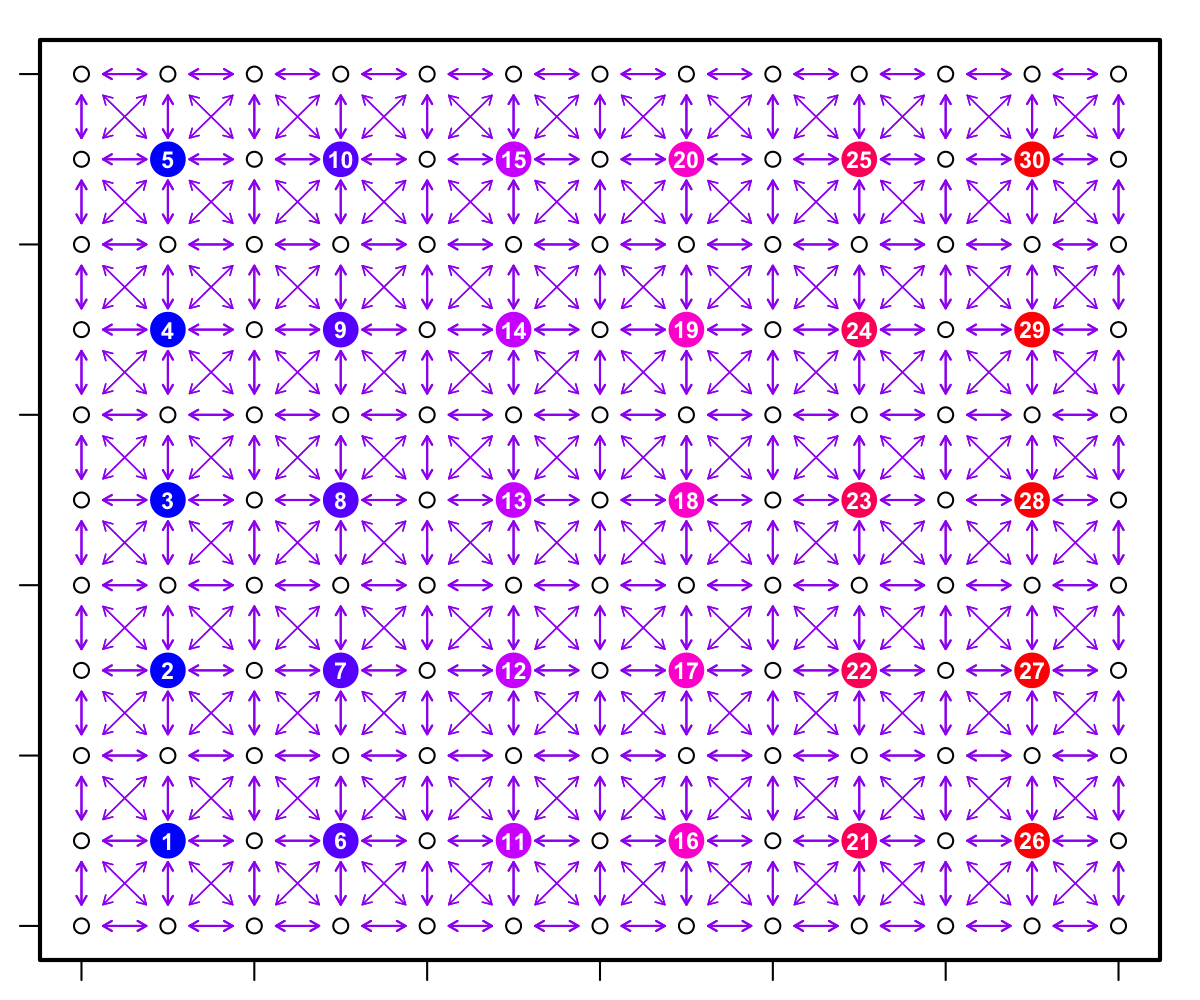
\includegraphics[width=2.8in,height=2.33in]{figs/sims/basic_lattice.png}}
		\subcaptionbox{lattice inference \label{lattice_inference}}
			{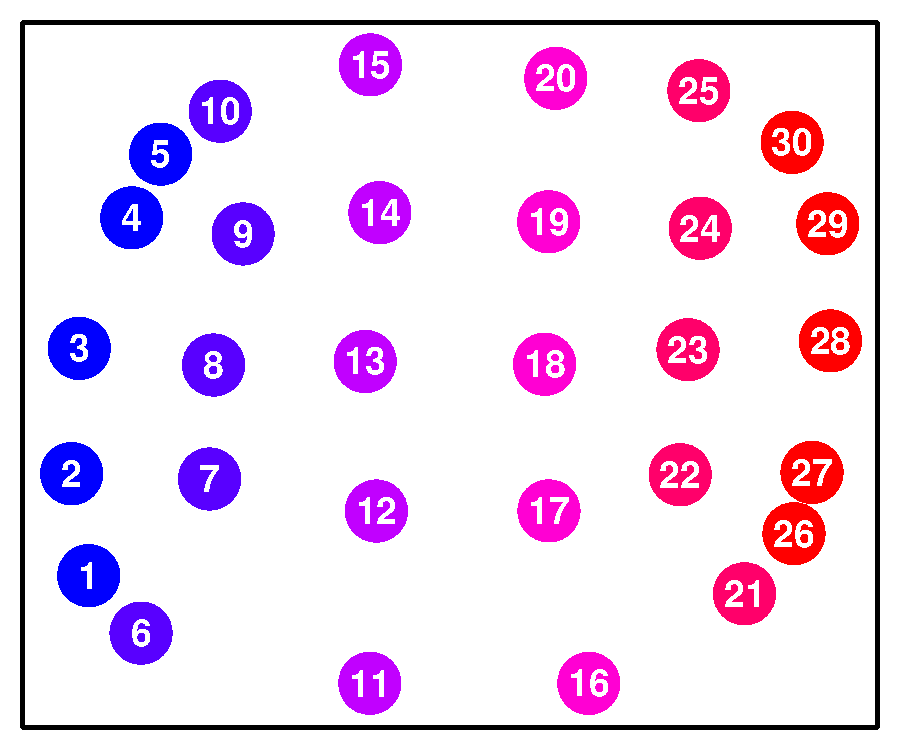
\includegraphics[width=2.8in,height=2.33in]{figs/sims/GeoGenMap_lattice.pdf}}
	\caption{Simulation scenarios and SpaceMix inference.  a) configuration of simulated populations on a simple lattice at equilibrium; b) inference of population locations under this scenario.}\label{sfig:lattice_scenarios}
\end{figure}

In the first scenario (output illustrated in Fig. \ref{sfig:lattice_scenarios}\subref{lattice_inference}), we simulate a stepping stone model at migration-drift equilibrium with homogeneous migration rates across the grid. In Figure \ref{sfig:lattice_scenarios}\subref{lattice_inference}, the reader can see that the configuration estimated for the populations by SpaceMix matches the lattice structure used to simulate the data, and that populations are correctly choosing their nearest neighbors.  Populations at the edge of the lattice have the least amount of data informing their exact placement, and are therefore pulled in somewhat.

\begin{figure}
	\centering
		\subcaptionbox{simulated lattice with barrier \label{barrier_lattice}}
			{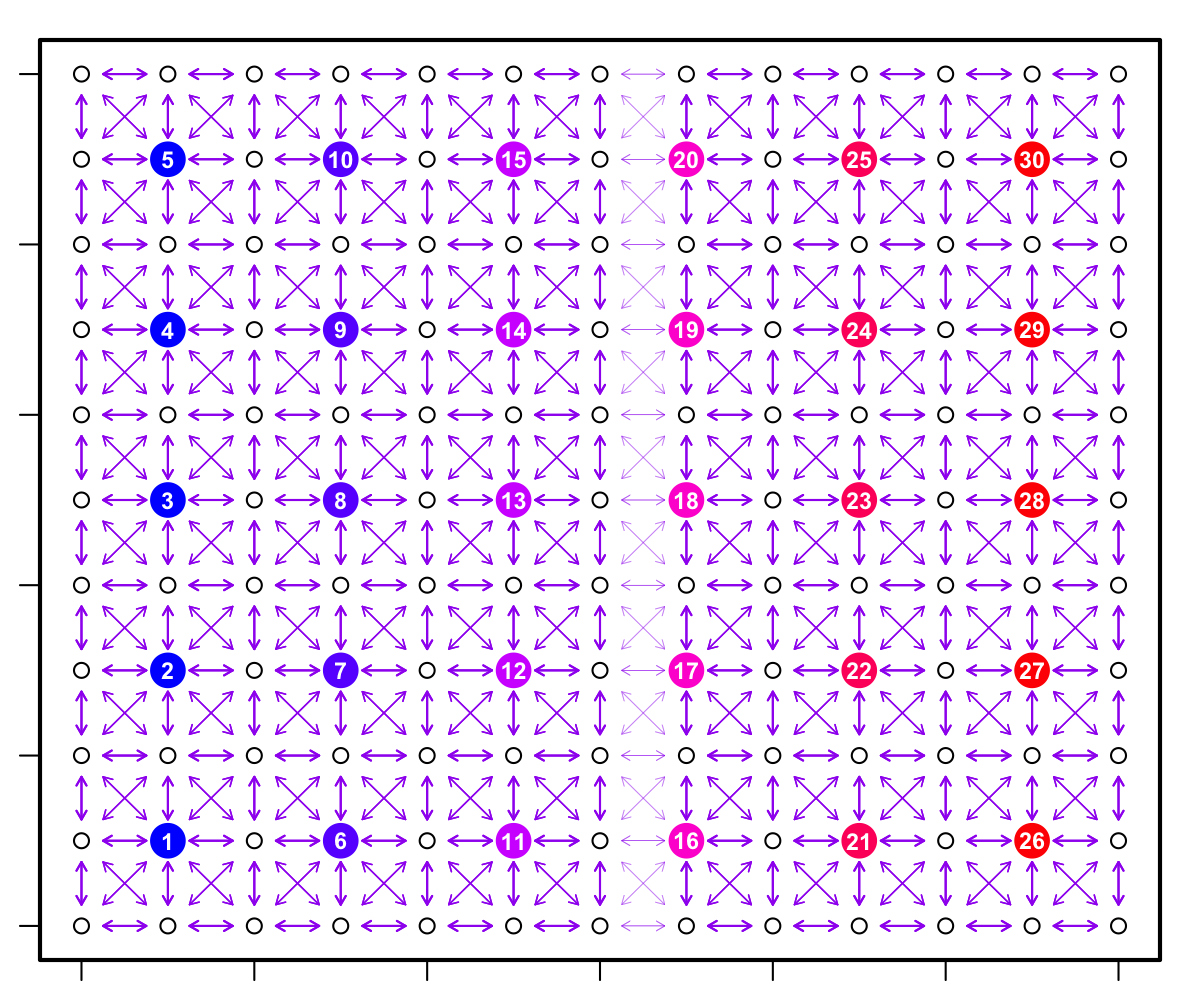
\includegraphics[width=2.8in,height=2.33in]{figs/sims/barrier_lattice.png}}
		\subcaptionbox{barrier inference\label{barrier_inference}}
			{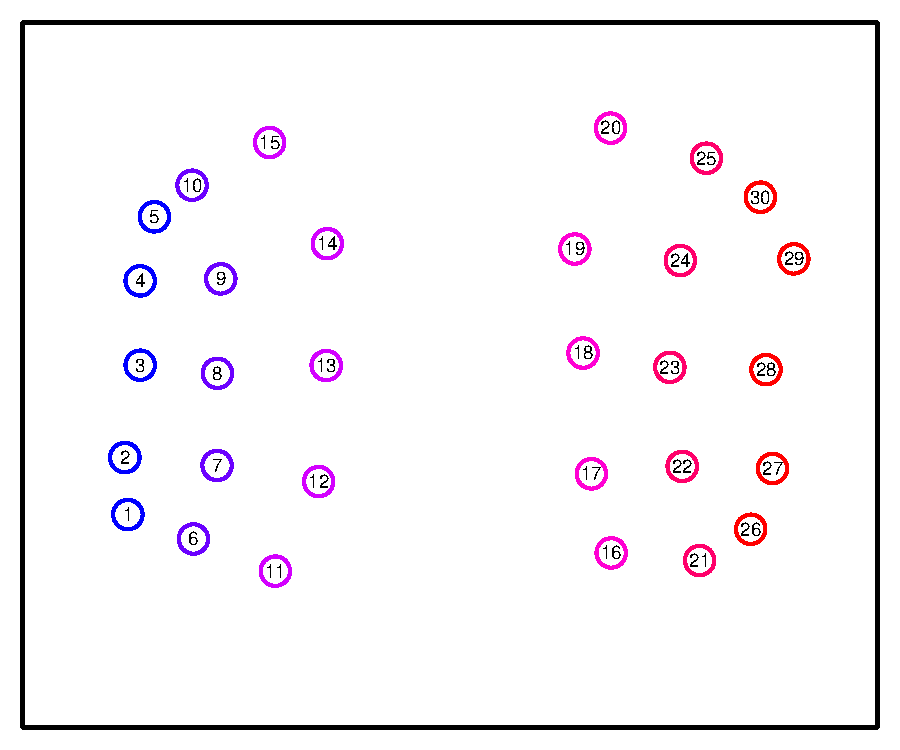
\includegraphics[width=2.8in,height=2.33in]{figs/sims/GeoGenMap_barrier.pdf}}
	\caption{Simulation scenarios and SpaceMix inference.  a) a lattice with a barrier across the center line of longitude; b) inference of population locations under this scenario.}\label{sfig:barrier_scenarios}
\end{figure}

In our second scenario (Fig. \ref{sfig:barrier_scenarios}\subref{barrier_inference}), we simulate under the same stepping stone model, but introduce a longitudinal barrier to dispersal (between populations 11:15 and 16:20), across which migration rates are attenuated by a factor of 5.  In Figure \ref{sfig:barrier_scenarios}\subref{barrier_inference}, the population configuration matches that of the lattice used to simulate the data, but due to the influence of the barrier, the two halves of the map have pushed farther away from one another.  This gap between populations on either side of the barrier reflects the way those populations perceive the increased effective distance between them.

\begin{figure}
	\centering
		\subcaptionbox{simulated lattice with expansion \label{expansion_lattice}}
			{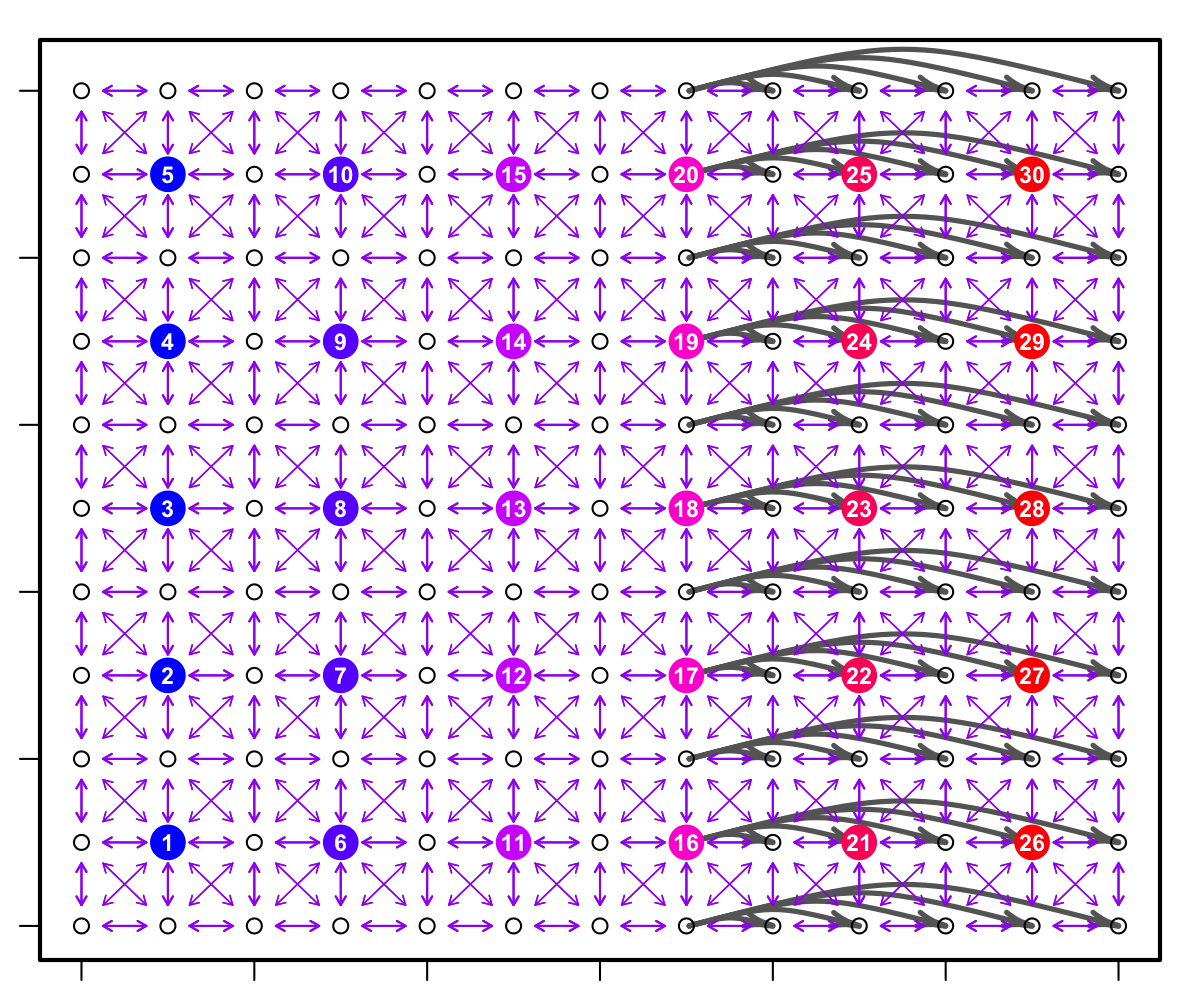
\includegraphics[width=2.8in,height=2.33in]{figs/sims/expansion_lattice.png}}
		\subcaptionbox{Expansion  \label{expansion_inference}}
			{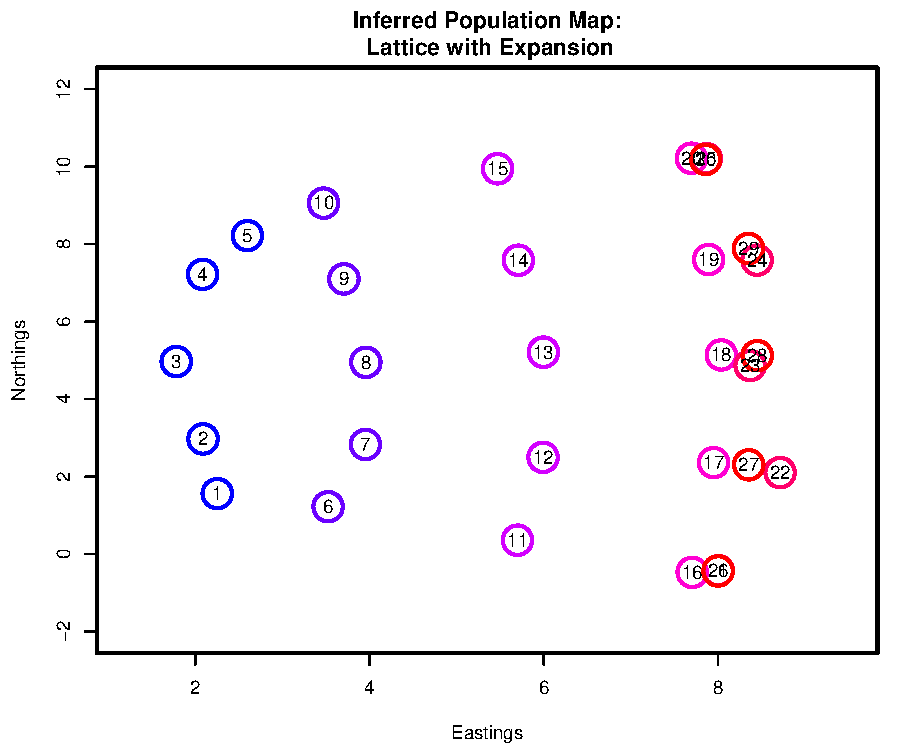
\includegraphics[width=2.8in,height=2.33in]{figs/sims/GeoGenMap_expansion.pdf}}
	\caption{Simulation scenarios and SpaceMix inference.  a) a lattice with recent expansion on the eastern margin; b) inference of population locations under this scenario.}\label{sfig:expansion_scenarios}
\end{figure}

In the third scenario (Fig. \ref{sfig:expansion_scenarios}\subref{expansion_inference}), we simulate an expansion event in which all populations in the last five columns of the grid have expanded in the recent past from the nearest population in their row (e.g., populations 25 and 30, as well as the three unsampled populations that bracket them, have all expanded at the same point in the recent past from population 20). In the scenario of recent expansion (Fig. \ref{sfig:expansion_scenarios}\subref{expansion_inference}), the daughter populations of the expansion event cluster with their parent populations, reflecting the higher relatedness (per unit geographic separation) between them.  In SuppMat Figs \ref{sfig:sim_covariance_decays}, we show the relationship between covariance in allele frequencies and geographic distance and inferred geogenetic distance for these simulations.

%referring to Fig. \ref{sfig:lattice_scenarios}\subref{simple_lattice},

If our data are well fit by a model of isolation by distance, then (1) a population's genetic makeup should be well predicted by that of its neighbors, and (2) populations should not show excess covariance with distant populations. Violation of either of these two points will result in a poor fit of a simple isolation by distance model, and particularly a violation of point (2) may indicate that long distance admixture has taken place.

To examine the behavior of SpaceMix when there is long distance covariance between populations, we simulated an admixture event on the stepping-stone model we had used previously.  Specifically, (using Fig. \ref{sfig:corner_admix_scenarios}\subref{corner_admixture_lattice} as a reference) we allowed population 30, in the northeast corner of the grid, to draw half of its ancestry from population 1, in the southwest corner.  The result of a SpaceMix analysis in which the locations of these populations were estimated is shown in Figure \ref{sfig:corner_admix_scenarios}\subref{corner_admix_inference_CYOL}.

\begin{figure}
	\centering
		\subcaptionbox{simulated lattice with admixture \label{corner_admixture_lattice}}
			{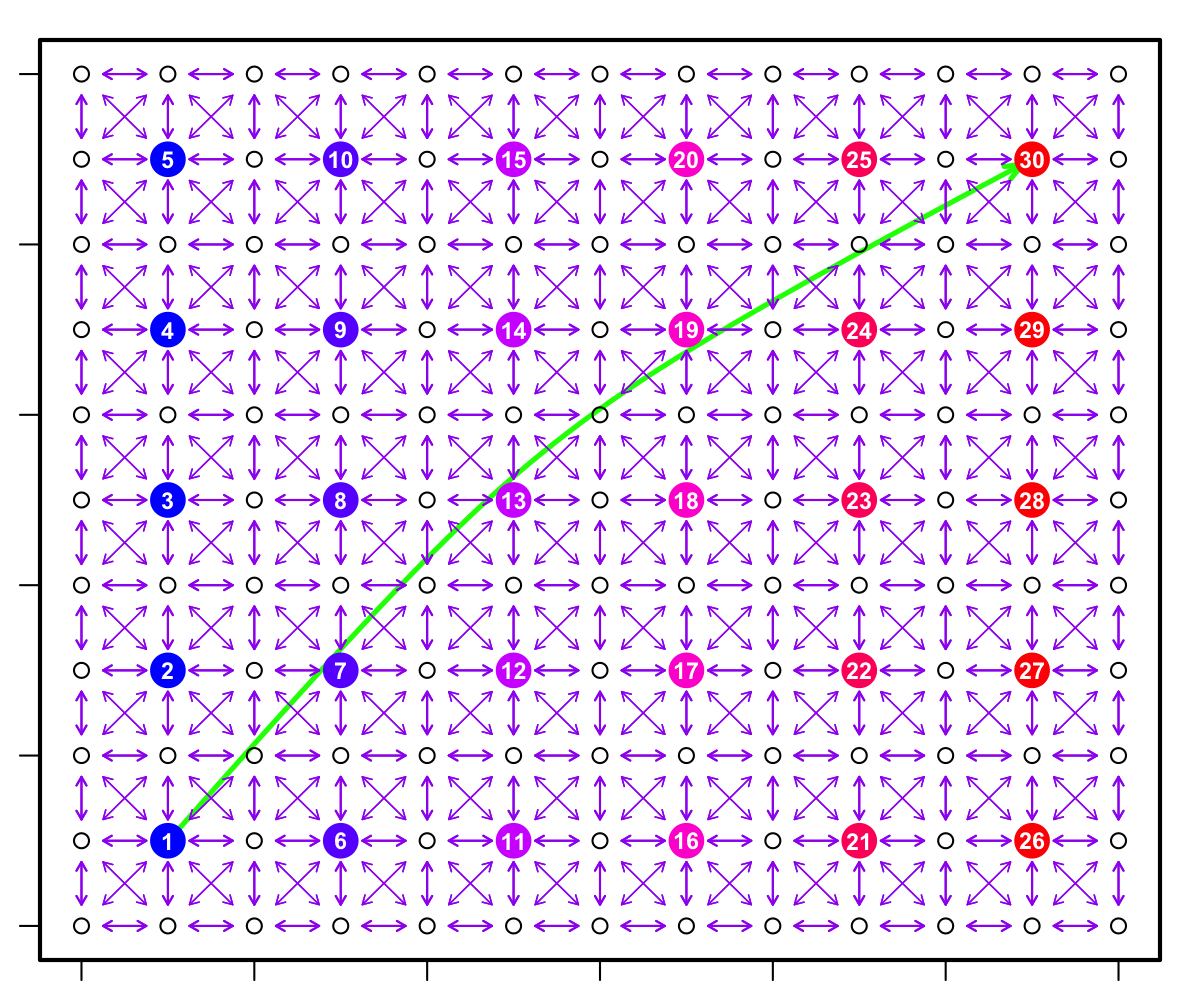
\includegraphics[width=2.8in,height=2.33in]{figs/sims/corner_admixture_lattice.png}}
		\subcaptionbox{location Inference \label{corner_admix_inference_CYOL}}
			{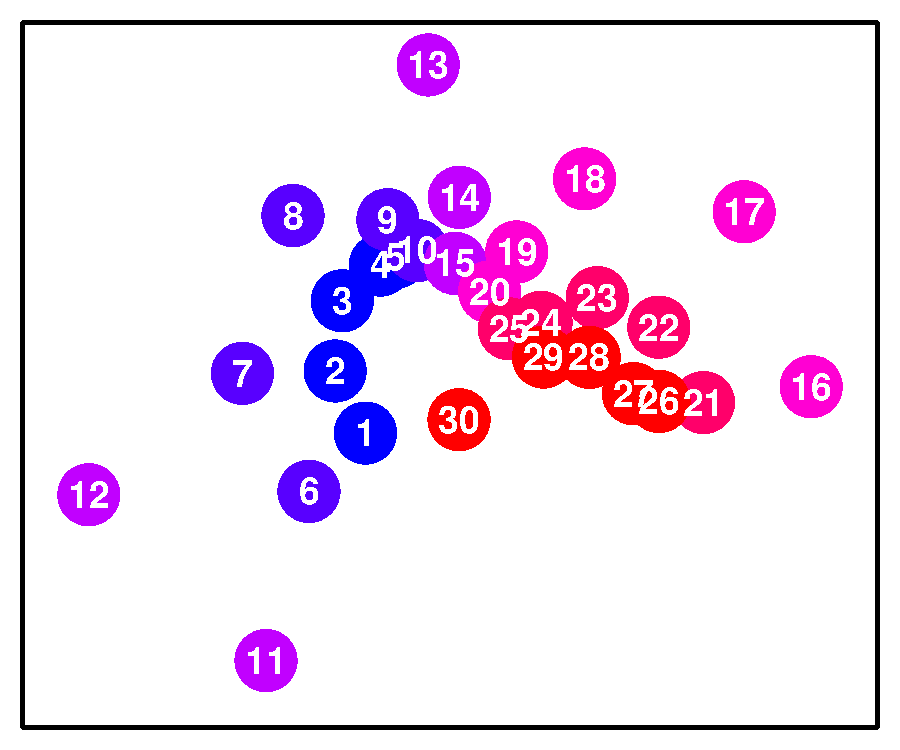
\includegraphics[width=2.8in,height=2.33in]{figs/sims/GeoGenMap_corner_admixture_CYOL.pdf}}
		\subcaptionbox{location and admixture inference  \label{corner_admix_inference}}
			{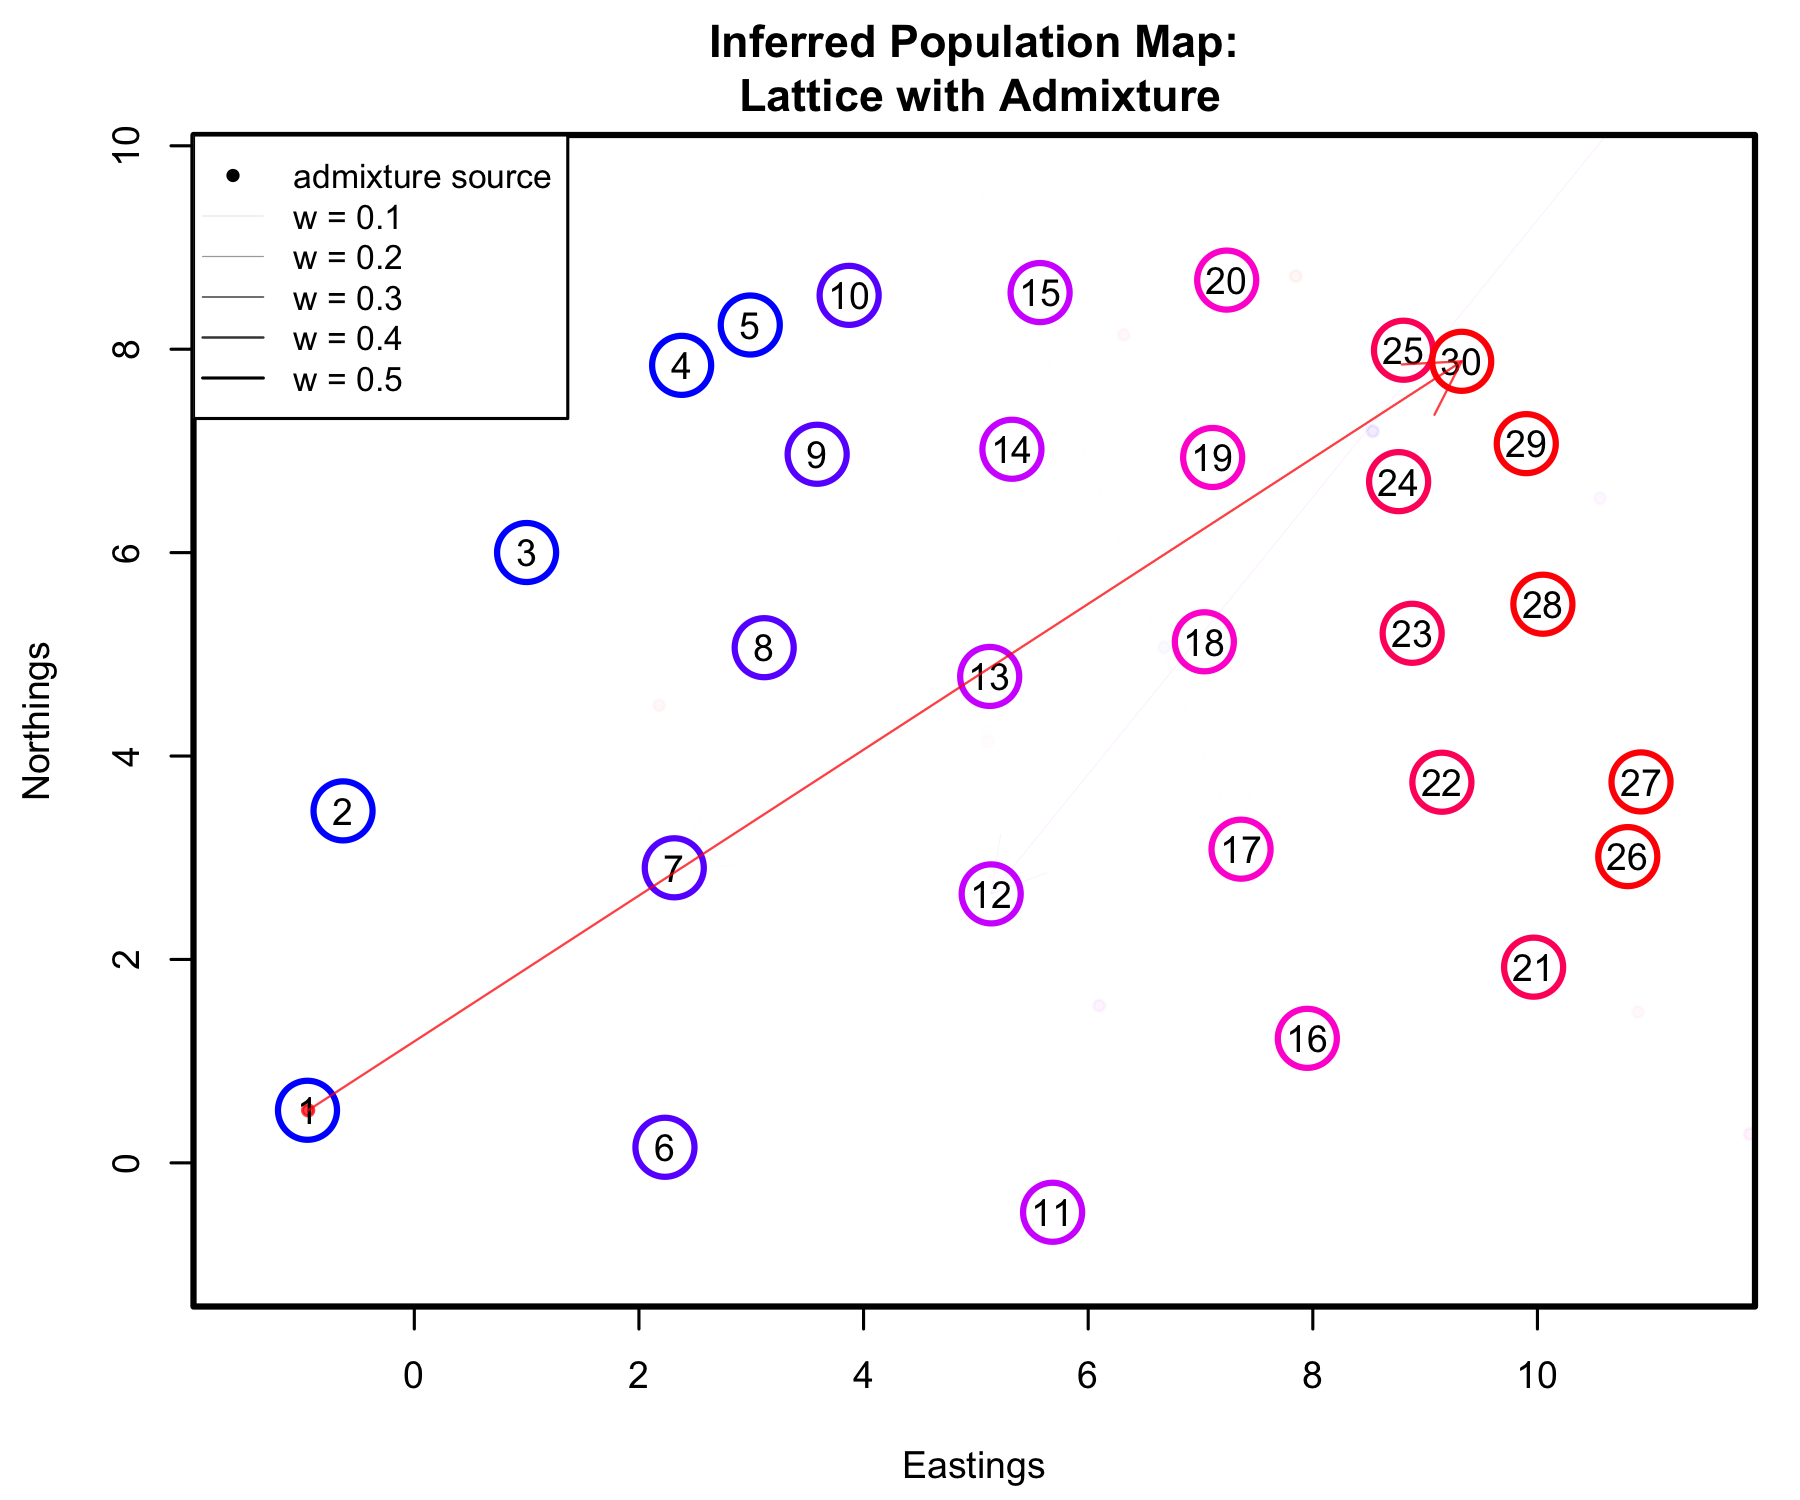
\includegraphics[width=2.8in,height=2.33in]{figs/sims/GeoGenMap_corner_admixture.png}}
	\caption{Simulation scenarios and SpaceMix inference.  a) a lattice with recent admixture event between population 1 in the southwest corner and population 30 in the northeast corner; b) inference of population locations under this scenario; c) inference of population locations and their sources of admixture under this scenario.}\label{sfig:corner_admix_scenarios}
\end{figure}

This signal of excess covariance over anomalously long distances is clearly difficult to accommodate within the ``choose-your-own-location" framework described above.  In Figure \ref{sfig:corner_admix_scenarios}\subref{corner_admix_inference_CYOL}, the reader can see the torturous lengths to which the method goes to come up with a configuration of populations that accommodates their genetic relationships.  The admixed population 30 is estimated to have a location intermediate between population 1, the source of its admixture, and populations 24, 25, and 29, the nearest neighbors to the location of its non-admixed portion.  However, this warping of space is difficult to interpret, and would be especially so in the visualization of genetic relationships in empirical data for which a researcher does not know the true demographic history.  It would therefore be of great utility to directly model the action of admixture on spatial patterns of genetic variation.

%%%%%%%%% %%%%%%%%% 
\subsection*{Inference of Spatial Admixture}
We can incorporate recent admixture directly into out inference framework.  We imagine that population $k$ draws the majority of its ancestry from $G^{\prime}_{k}$, but that a proportion $0 \geq w_k \leq 0.5$ of its ancestry comes from another location \kadmixsource{k}, which we refer to as its source of admixture. The mean standardized population allele frequency at locus $\ell$ in population $k$ is a weighted average of the allele frequencies at the geographic location of the sampled population chooses for itself ($p_{\ell,k'}$) and those at the coordinates of the source ($p_{\ell,\identifyadmixsource{k}}$) from which the observed population draws admixture:
\begin{equation}
w_k p_{\ell,k'} + (1-w_k) p_{\ell,\identifyadmixsource{k}} \label{eqn-admixedfreq}
\end{equation}
We can allow each of our populations to have an independent spatial source of admixture. Our $p_{\ell,k'}$ and $p_{\ell,\identifyadmixsource{k}} $ are well defined, as, given our population allele frequency covariance matrix, equation \ref{eq:spatial_covariance}, we can get the distribution of allele frequencies at any point in space simply by plugging its spatial coordinates into our $\Omega(D(G))$.

We can then consider the resulting parametric covariance matrix that follows from the form of the population frequencies in equation \eqref{eqn-admixedfreq}. The covariance between the standardized allele frequencies of population $i$ and $j$ can be modeled as 
\begin{alignat}{3}
\label{eq:admixed_covariance_1}
\identifyadmixsource{\Omega_{i,j}} = (1-w_i)(1-w_j) \Omega_{i\;,\;j\;} \; \times&\\
(w_i)(1-w_j) \Omega_{\identifyadmixsource{i},\;j\;} \; \times   \notag&\\
(w_j)(1-w_i) \Omega_{i\;,\;\identifyadmixsource{j}} \; \times   \notag&\\
(w_i)(w_j) \Omega_{\identifyadmixsource{i},\;\identifyadmixsource{j}} \; +   \notag&\\
\delta_{i,j} (\eta_i + \bar{S}^{-1}) \notag&
\end{alignat}
where $\identifyadmixsource{i}$ and $\identifyadmixsource{j}$ are the sources from which populations $i$ and $j$ are drawing their admixture with proportions $p_i$ and $p_j$, and the spatial covariance function of population frequencies, $\Omega$, is given by \eqref{eq:spatial_covariance} (this lacks the sample-specific variance terms on the diagonal). Note that we then reintroduce the nugget, $\eta_k$, and the sample size effect, $\bar{S_k}^{-1}$, for each population, to model drift or excess variance in population $k$ on top of that predicted by the mixture of frequencies given by our spatial model.  As in equation \eqref{eq:spatial_covariance2}, $\delta_{i,j} $ is the indicator function $1$ if $i=j$, and $0$ otherwise. 

%parameterized by the pairwise geographic distances between each pair of populations, \emph{without} the population-specific variance terms on the diagonal (i.e., in equation \eqref{eq:admixed_covariance_1}, i.e.\ $\Omega_{i,j} = \frac{1}{\alpha_0} \text{exp} \left(	\left( \alpha_1D_{i,j} \right)^{\alpha_2} \right)$).  

The admixed covariance between samples $i$ and $j$, $\identifyadmixsource{\Omega_{i,j}}$ is then a function of all the pairwise spatial covariances between populations $i$ and $j$ and the points from which they draw admixture, $\identifyadmixsource{i}$ and $\identifyadmixsource{j}$.  Those spatial covariances in turn are a function of all combinations of pairwise distances between their locations: $G_i$, $G_j$, \kadmixsource{i}, and \kadmixsource{j}.  This parametric covariance form is illustrated in Figure \ref{sfig:admixed_cov_diagram}.

As we only get to observe the sample frequencies and we standardize our allele frequencies using the sample mean, our predicted admixture covariance matrix needs to be transformed to accommodate these sampling considerations. We can do this as before (see Methods), and we again treat the likelihood of our sample covariance matrix as Wishart:
\begin{equation}
\label{eq:wishart_dist_admixed}
P(\widehat{\Omega} \mid \identifyadmixsource{\Omega}) = 
	\mathcal{W}\left(L \widehat{\Omega} \mid \identifyadmixsource{\Omega} \left( G',\identifyadmixsource{G}, w,\vec{\alpha},\eta \right),L \right)	\text{.}
\end{equation}
As before $G'$, $\vec{\alpha}$, $\eta$ are treated as random variables to be estimated. Now the set of $K$ admixture sources $\identifyadmixsource{G}$ are also parameters to be estimated, along with the vector of $K$ admixture proportions, $w$. The posterior probability of these parameters can be expressed as a function of this parametric admixed covariance, $\identifyadmixsource{\Omega}$,
\begin{equation}
\label{eq:admixed_post_prob}
P(G',\identifyadmixsource{G}, w,\vec{\alpha}, \eta \mid \widehat{\Omega}, L,G) 
	\propto  
		P(\widehat{\Omega}  \mid \identifyadmixsource{\Omega}) P(\vec{\alpha}) P(G') P(\identifyadmixsource{G}) P(w) P(\eta) 
\end{equation}
%
as specified by the parameters $w$, $\identifyadmixsource{G}$, $\vec{\alpha}$, and $\eta$, and the observed locations, $G$.  We place the same priors as stated above on $G^{\prime}$, $\vec{\alpha}$, $\eta$, and we now specify priors on $w$ and $\identifyadmixsource{G}$.  The admixture proportions, $w$, are capped at 0.5, to prevent populations from swapping identities with their source of admixture, and are heavily weighted towards small values to be conservative with respect to admixture inference.  Our admixture proportions are independently beta-distributed: $2 w_k \sim \beta(\alpha = 1,\beta = 100)$.  The priors on the sources of admixture, $\identifyadmixsource{G}$ are taken independently as bivariate normal spatial distributions, all with the same mean at the centroid of the observed population locations, $G$, and variance equal to twice the mean pairwise observed distance:  $\identifyadmixsource{G_k} \sim \mathcal{N}(\mu = \bar{G},\sigma = 2 \bar{D}(G))$.

\begin{figure}[ht!]
	\centering
	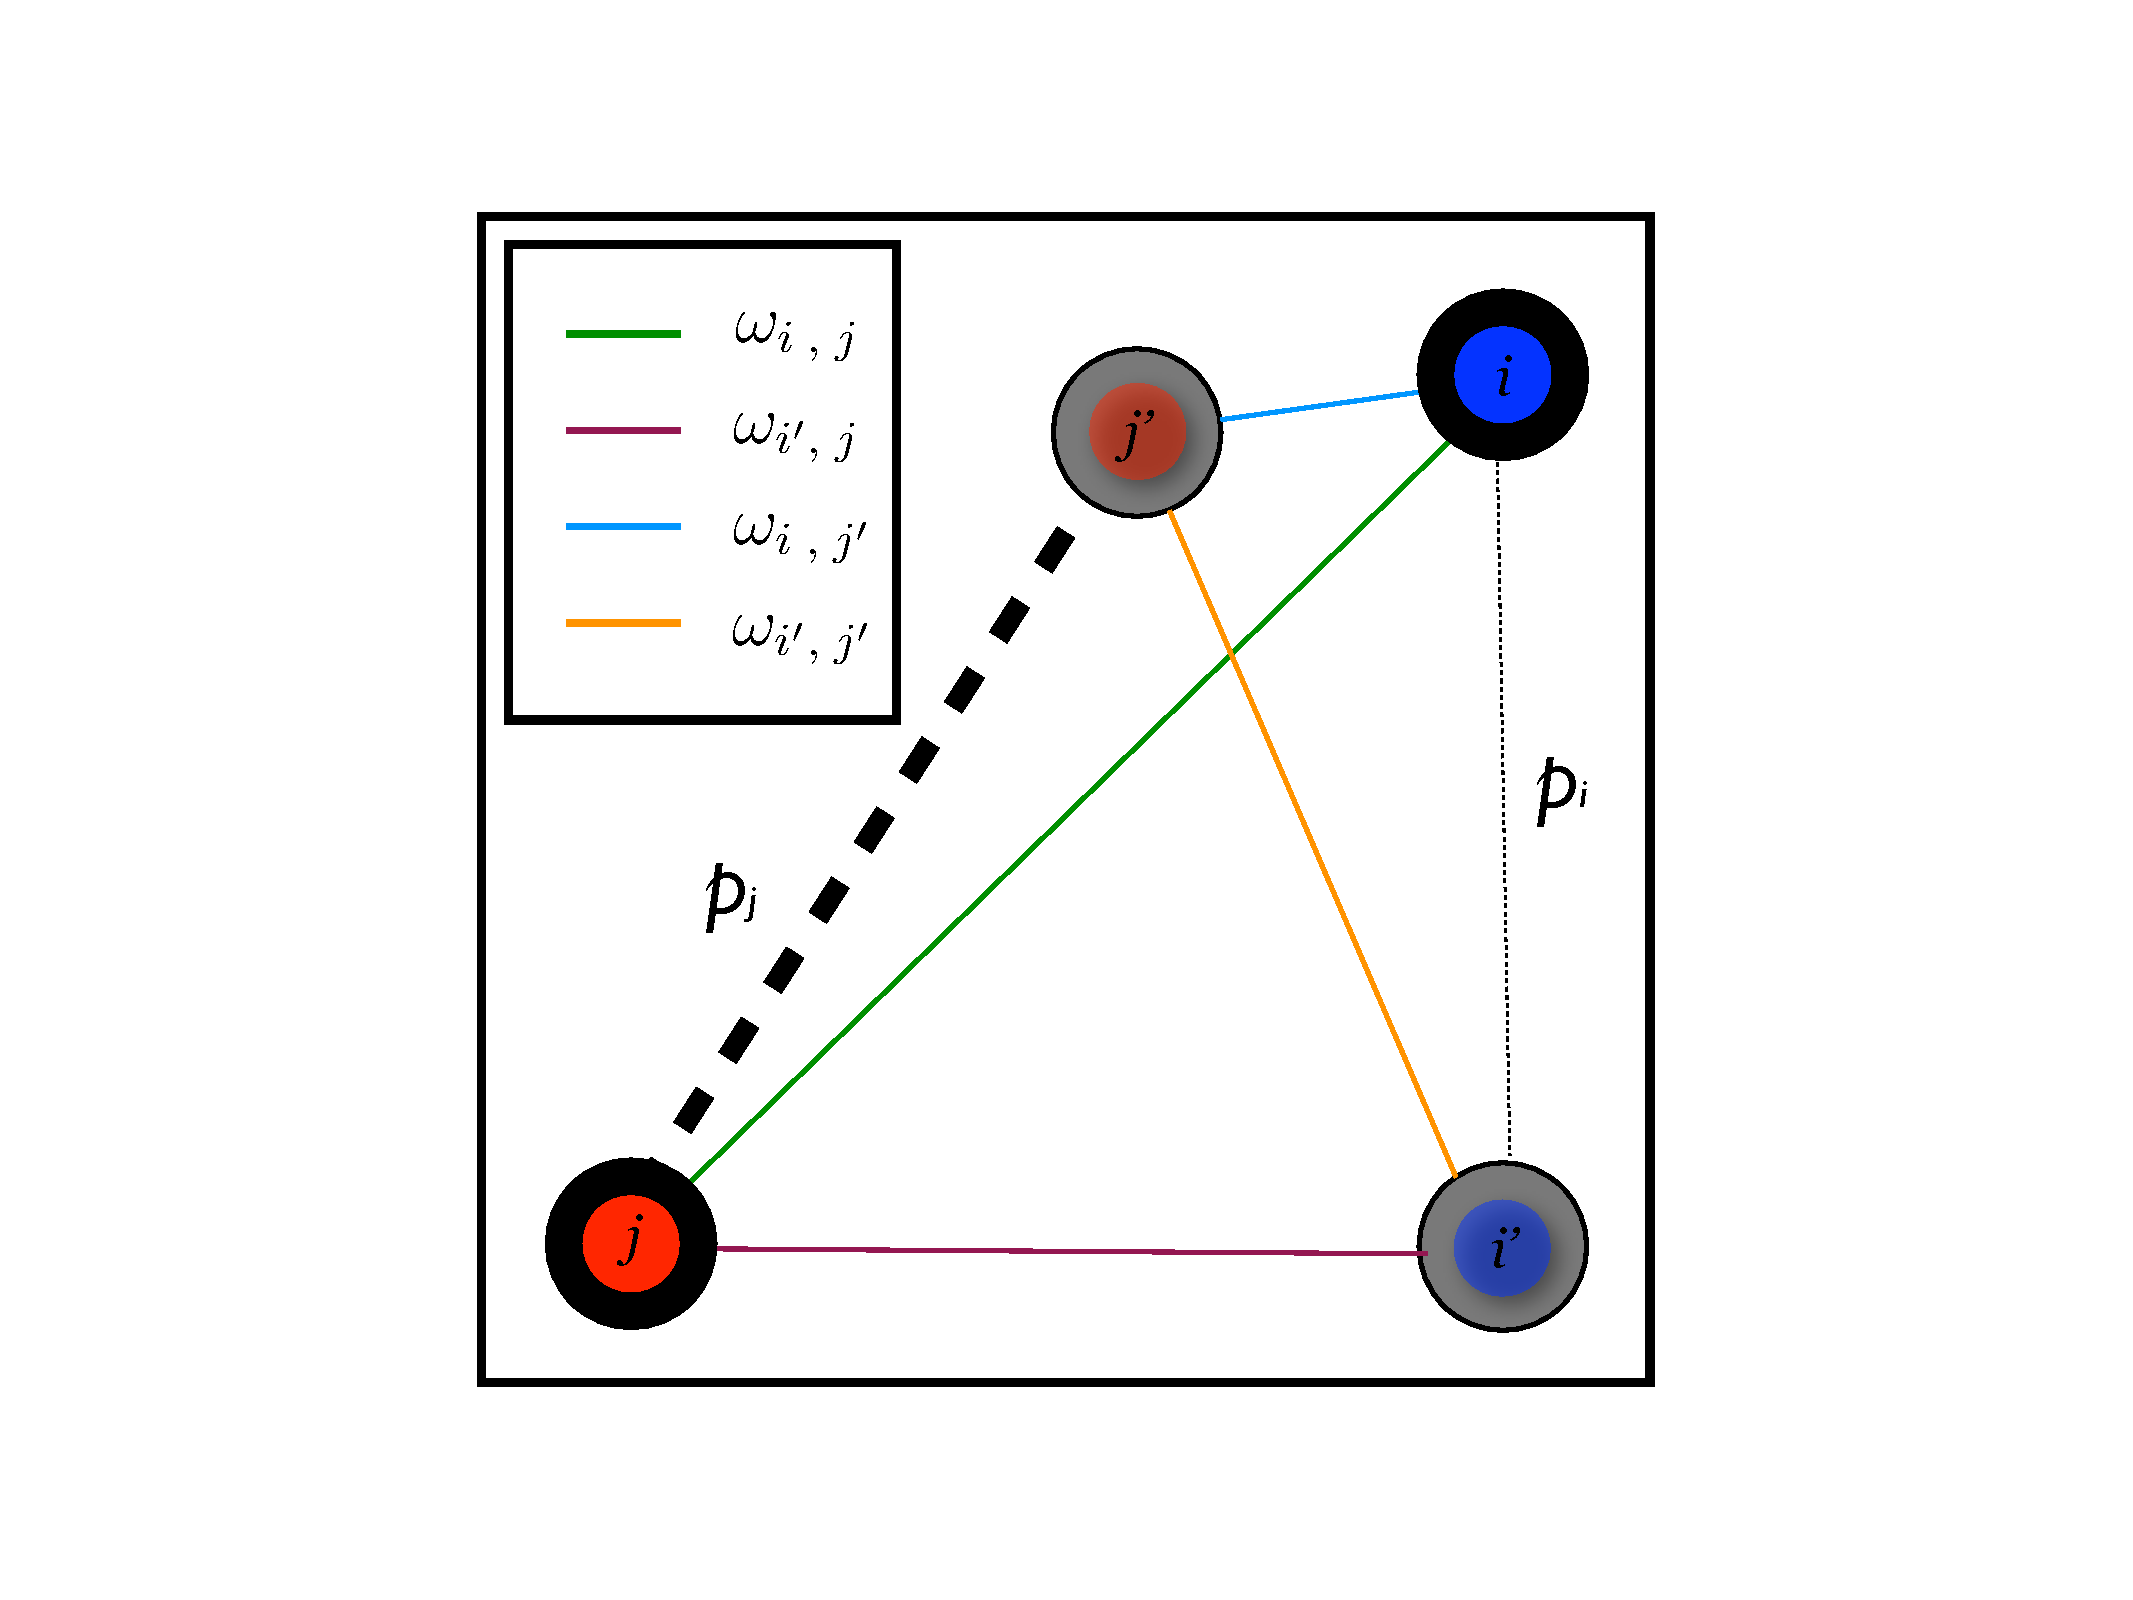
\includegraphics[width=2in,height=2in]{figs/admix_cov_fig.pdf}
	\caption{An illustration of the form of the admixed covariance given in equations \eqref{eq:admixed_covariance_1}.  Populations $i$ and $j$ are drawing admixture in proportions $p_i$ and $p_j$ from their respective sources of admixture, $\identifyadmixsource{i}$ and $\identifyadmixsource{j}$, and all pairwise spatial covariances (the $\Omega$'s) are shown.  In this cartoon example, population $j$ is drawing more admixture from its source $\identifyadmixsource{j}$ than $i$ is from its source $\identifyadmixsource{i}$ (i.e., $p_j > p_i$).}
\label{sfig:admixed_cov_diagram}
\end{figure}

%We treat the location of the source of admixture for population $k$, $\identifyadmixsource{G_k}$, and the population's admixture proportion, $p_k$, as random variables and jointly estimate them as part of our inference procedure. 

The models described above may be used in various combinations.  In the simplest model, populations do not choose their own locations, nor are they allowed to draw admixture, and the only parameters to be estimated are those of the spatial covariance function given in equation \eqref{eq:spatial_covariance}, and the population-specific variance terms ($\eta$).  In the most complex model, population locations, the locations of their sources of admixture, and the proportions of that admixture are all estimated jointly in addition to the parameters of the spatial covariance function and the population specific variances.  

An natural concern is whether all of these parameters are separately identifiable, most notably whether population locations, admixture locations, and proportions can be estimated. That is, if a population has received some level of admixture from another population, what is to stop it from simply moving toward that population in geogenetic space to satisfy its increased resemblance to that population, rather than choosing admixture from that location?

%\gb{Not sure what you were trying to say here.} The recent developments to test for admixture between populations using allele frequencies \citep{treemix}, rely on the fact that a population tree dictates particular conditions on the covariances of allele frequency differences among particular parts of the tree. Violations of these conditions allow for admixture to be identified, and also highlight conditions under which these tests may be misled (ancient population structure). 
Admixture is identifiable in our model because there are covariance relationships among populations that cannot simply be satisfied by shifting population locations around (as demonstrated by the tortured nature of Figure \ref{sfig:corner_admix_scenarios}\subref{corner_admix_inference_CYOL}). To illustrate this point, consider the simple spatial admixture scenario shown in Figure \ref{sfig:toy_admixture}. Our populations A-D are spatially arrayed  along a line, and their allele frequencies are specified by a simple isolation by distance model, but there is recent admixture from D into B (such that 40\% of the alleles in B are drawn from D). The lines show the expected covariance under IBD that each population (A, C, or D, as indicated by line color) has with a putative population at a given distance.  The dots show the resulting admixed covariance between B and the three other populations, as well as B's variance with itself (B-B) as specified by equation \eqref{eq:admixed_covariance_1}, with no nugget or sampling effect.

\begin{figure}[ht!]
	\centering
	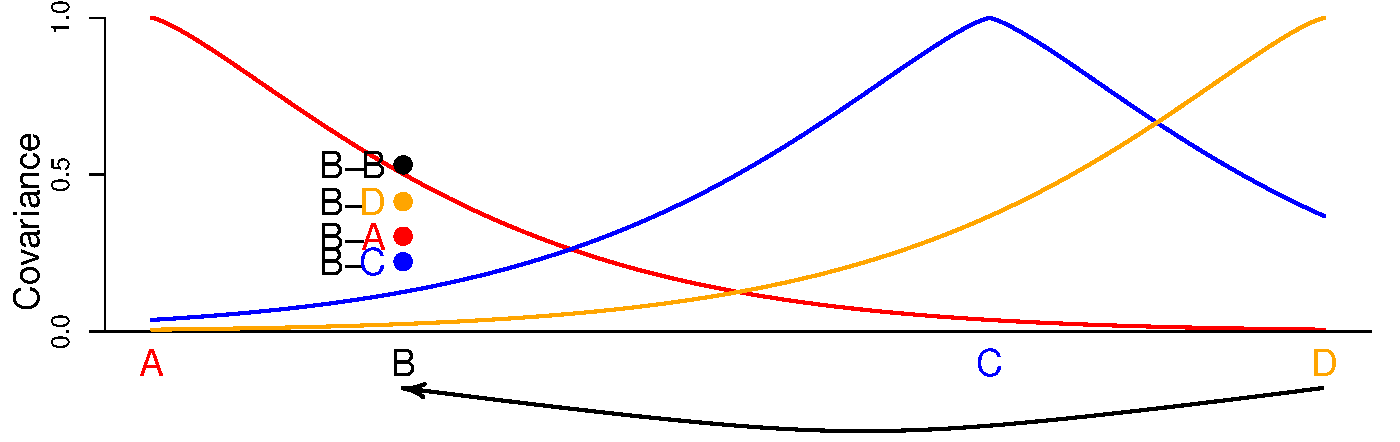
\includegraphics[width=\textwidth]{figs/sims/Admix_covar_toy_fig.pdf}
	\caption{} \label{sfig:toy_admixture}
\end{figure}

Due to its admixture from D, B has lower covariance with A than expected given its distance, somewhat higher covariance with C, and much higher covariance with D. In addition, the variance of B is lower than that of the other three populations, which each have variance $1$: the value of the covariance when the distance is zero. This lower variance results from the fact that the frequencies at $B$ represent a mixture of the frequency at $D$ and the frequency at $B$ before the admixture. 

Now, using this example scenario, let us return to the concern posed above: that admixture location and population location are non identifiable.  For the sake of simplicity, assume that we hold the locations of A, C, and D constant, as well as the decay of covariance with distance (as could be the case if A-D are part of a larger analysis).  The covariance relationships of $B$ to the other populations cannot be simply satisfied by moving $B$ towards D. Doing so would better match B's covariance to D, but B would then have a covariance with C that is higher, and a covariance with A that is lower, than that we actually observe. 

Moving B also does not resolve the mystery that its variance is lower than that of the other populations. Introducing admixture into the model allows it to satisfy all of these conditions: it can draw ancestry from D but keep part of its resemblance to A, and it also avoids B having to move closer to C. Even in the absence of a sample from population C, B's covariance with A and D and its low variance could not be satisfied simply by moving B.  B is better described as a linear mixture of a population close to A and D.  However, there are specific scenarios in which a limited sampling scheme (both in size and location), can lead to non-identifiability between estimated population location and that of its source of admixture.  We describe an example of this phenomenon below.

We now return to the example admixture scenario described above in Figure \ref{sfig:corner_admix_scenarios}\subref{corner_admixture_lattice}, we demonstrate the inference of populations' sources and strengths of admixture and illustrate the results in Figure \ref{sfig:corner_admix_scenarios}\subref{corner_admix_inference}.  The reader can see that only the admixed population (population 30) is drawing admixture from the location of the source of admixture that was used to simulate the data, and that all other populations, which are not admixed, are choosing to draw admixture in only negligible amounts.

To demonstrate the use of the model in which the location of each population as well as the location of its source of admixture are estimated jointly, we used the spatial stepping-stone coalescent simulation procedure described above to generate a dataset of populations on a lattice in which there is both a barrier to dispersal and a more subtle admixture event (admixture proportion = 10\%, see Fig. \ref{sfig:barr_inland_ad}\subref{barr_inland_ad_scenario}).  In the SpaceMix analysis (Fig. \ref{sfig:barr_inland_ad}\subref{barr_inland_ad_inference}), the separation of the east and west sides of the grid accommodates the effect of the barrier to migration, and the admixed population (population 23) chooses admixture from very close to its true source (population 13), and in close to the correct amount ($\bar{p}_{(23)} = 0.05; 95\% \text{ credible interval} = 0.02-0.08$). 

%\gb{discuss how prior forces amount down, so it's cheaper to choose more westward pop as source}.

We also show a scenario in which there has been admixture (40\%) between two populations on either side of a barrier.  Here, the admixed population 23 is the only population that chooses a non-negligible proportion of admixture, but rather than drawing this admixture from its true source (population 13), it draws admixture from a location on the far margin of the half of the grid on its own side of the barrier.  The sampling scheme here illustrates more fully the example laid out in \ref{sfig:toy_admixture}: because there is no sampled intervening population between admixed population 23 and its source of admixture 13, there is nothing to stop 23 from explaining its higher covariance with 13 via its chosen location $G_{(23)}^{\prime}$ rather than via that of its source of admixture $\identifyadmixsource{G}_{(23)}$.  However, 23 still has a lower variance than the other populations, and therefore must choose a proportion of admixture to accommodate that fact.  This analysis is a somewhat artificial example, as the biological interpretation of ``admixture" (defined in our spatial framework as anomalously long distance covariance) between near neighbors is unclear.

\begin{figure}[ht!]
	\centering
		\subcaptionbox{`inland' admixture\label{barr_inland_ad_scenario}}
			{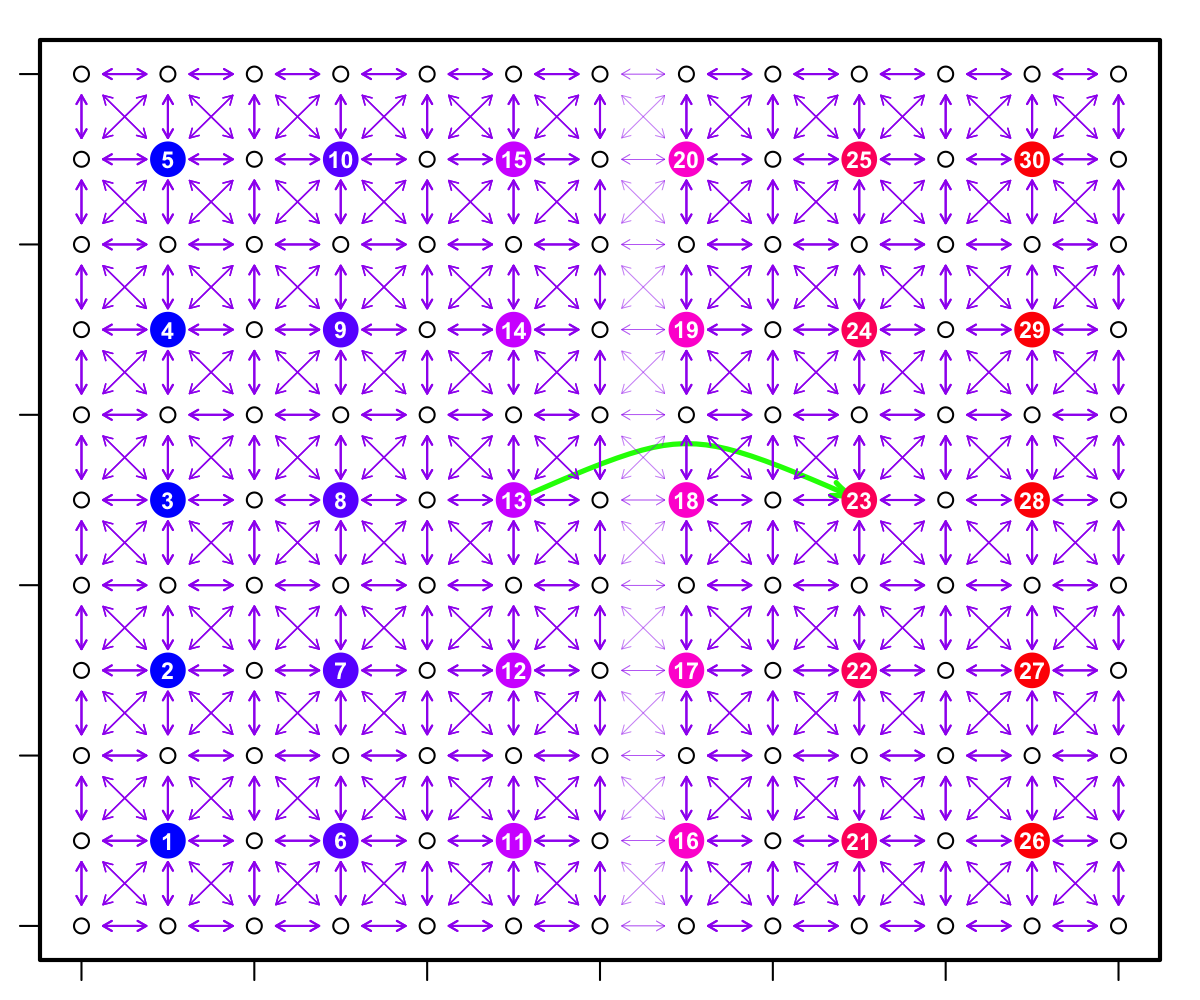
\includegraphics[width=2in,height=1.66in]{figs/sims/barr_indland_ad_lattice.png}}
		\subcaptionbox{inference \label{barr_inland_ad_inference}}
			{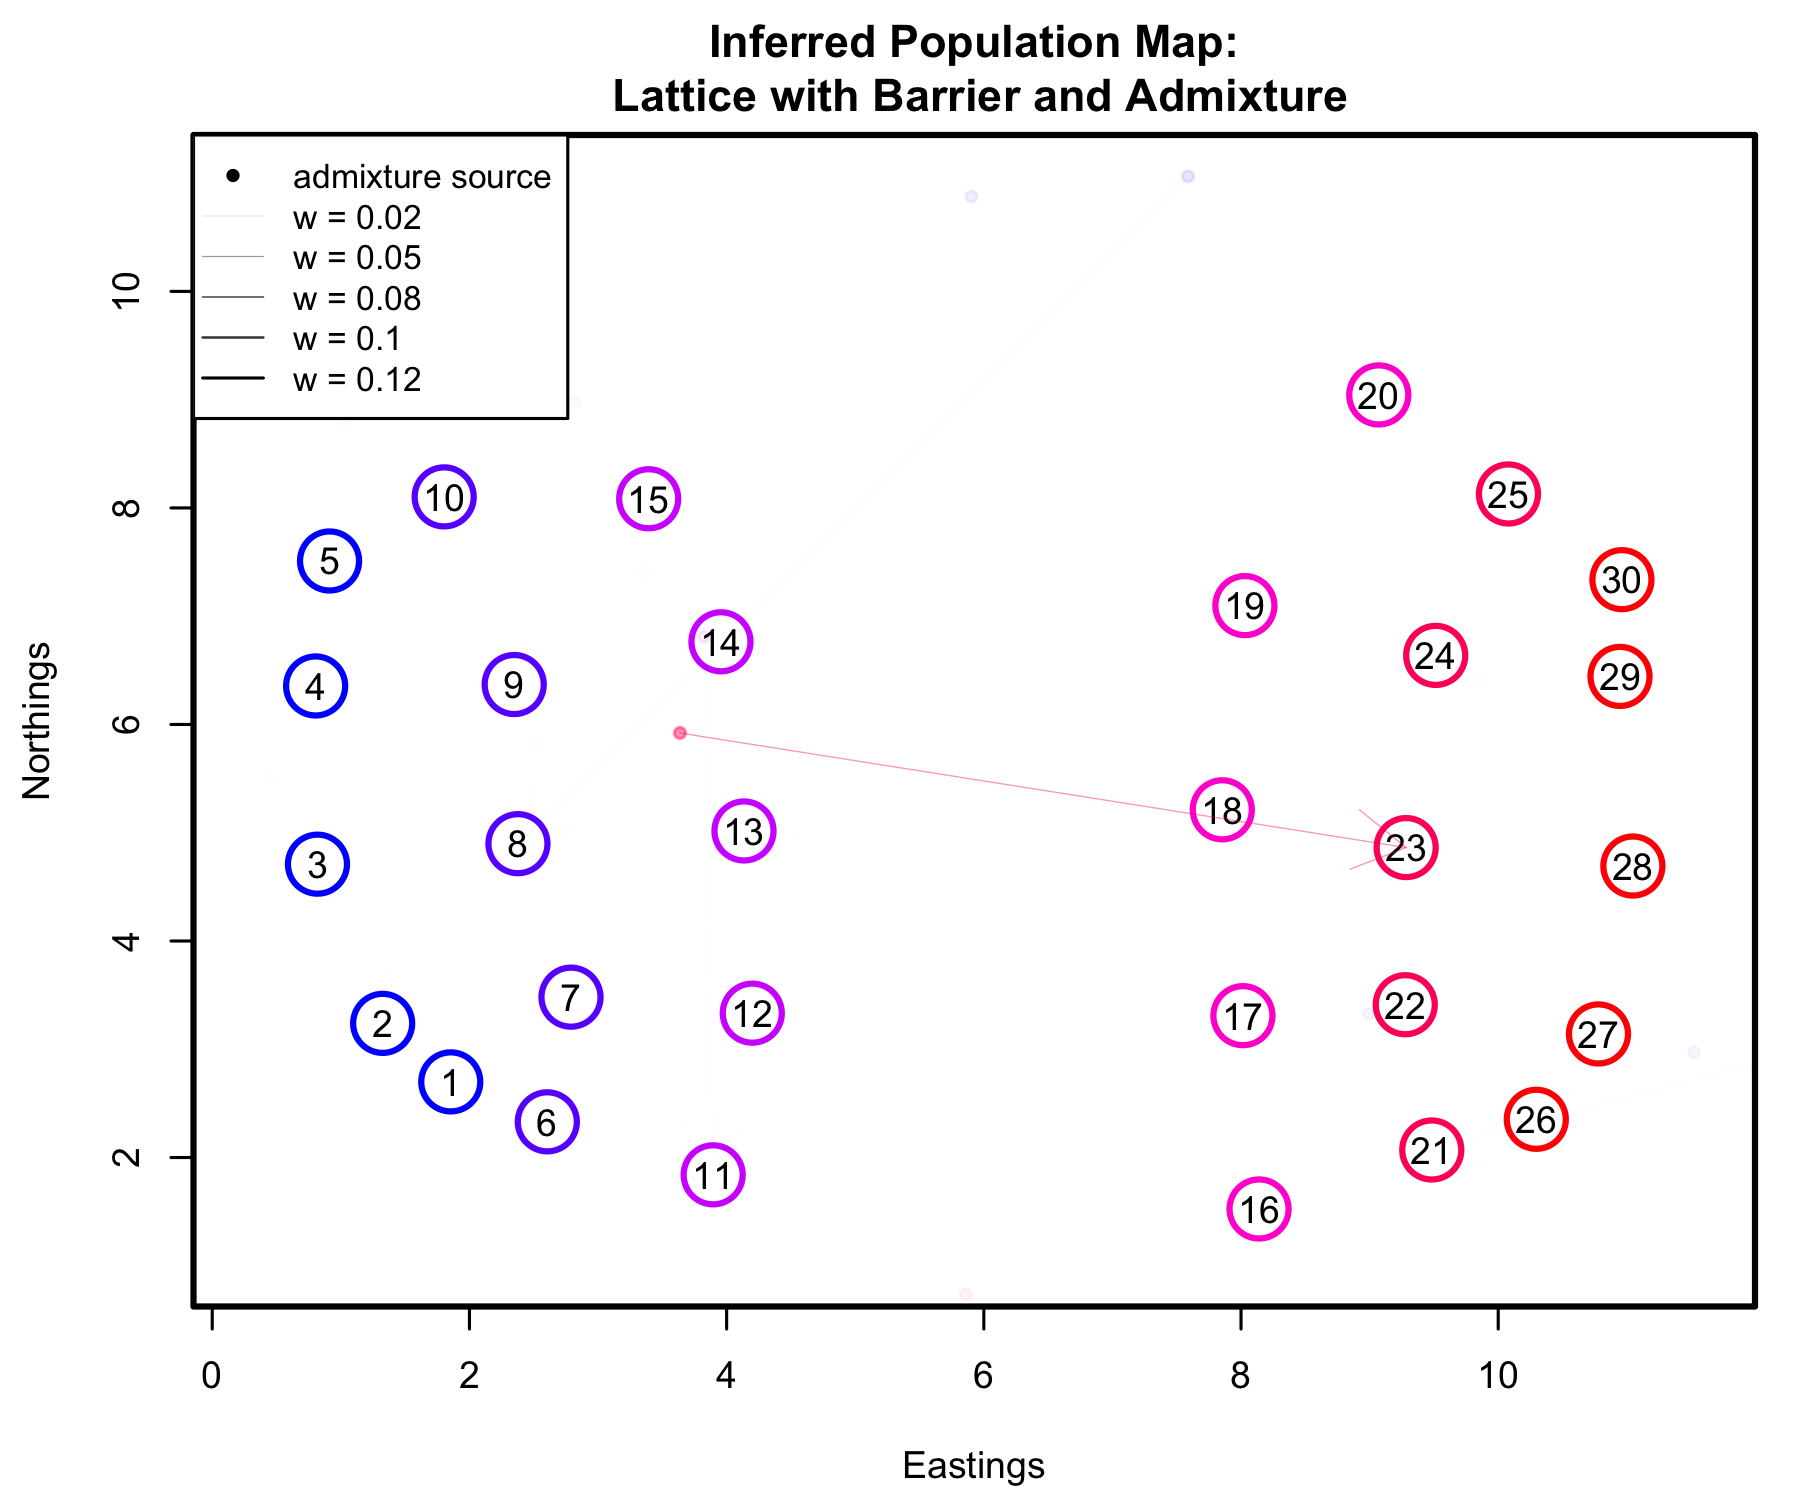
\includegraphics[width=2in,height=1.66in]{figs/sims/GeoGenMap_barr_inland_admixture_1.png}}
		\subcaptionbox{`neighbor' admixture \label{big_barr_ad_scenario}}
			{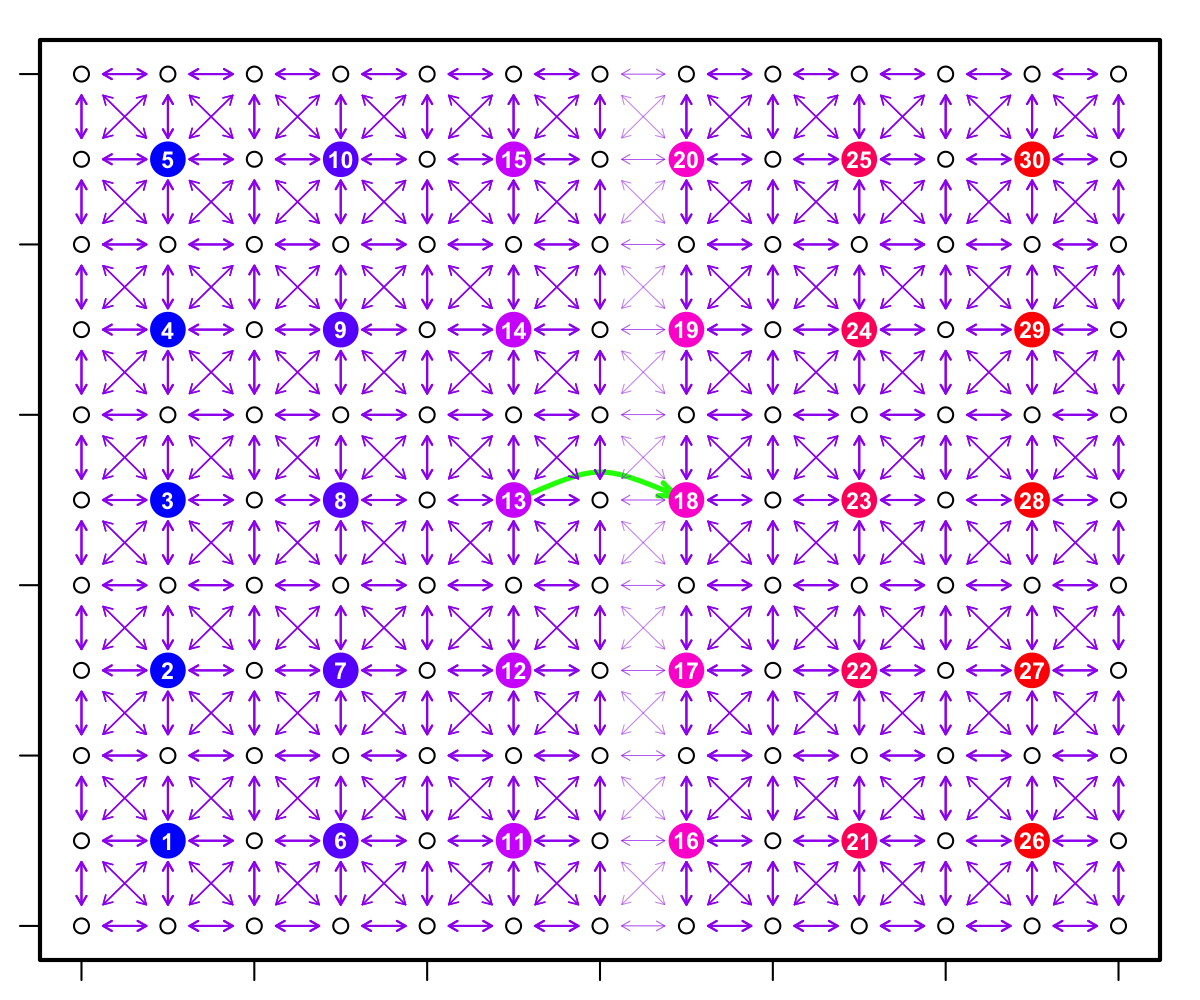
\includegraphics[width=2in,height=1.66in]{figs/sims/big_barr_ad_lattice.png}}
		\subcaptionbox{inference \label{big_barr_ad_inference}}
			{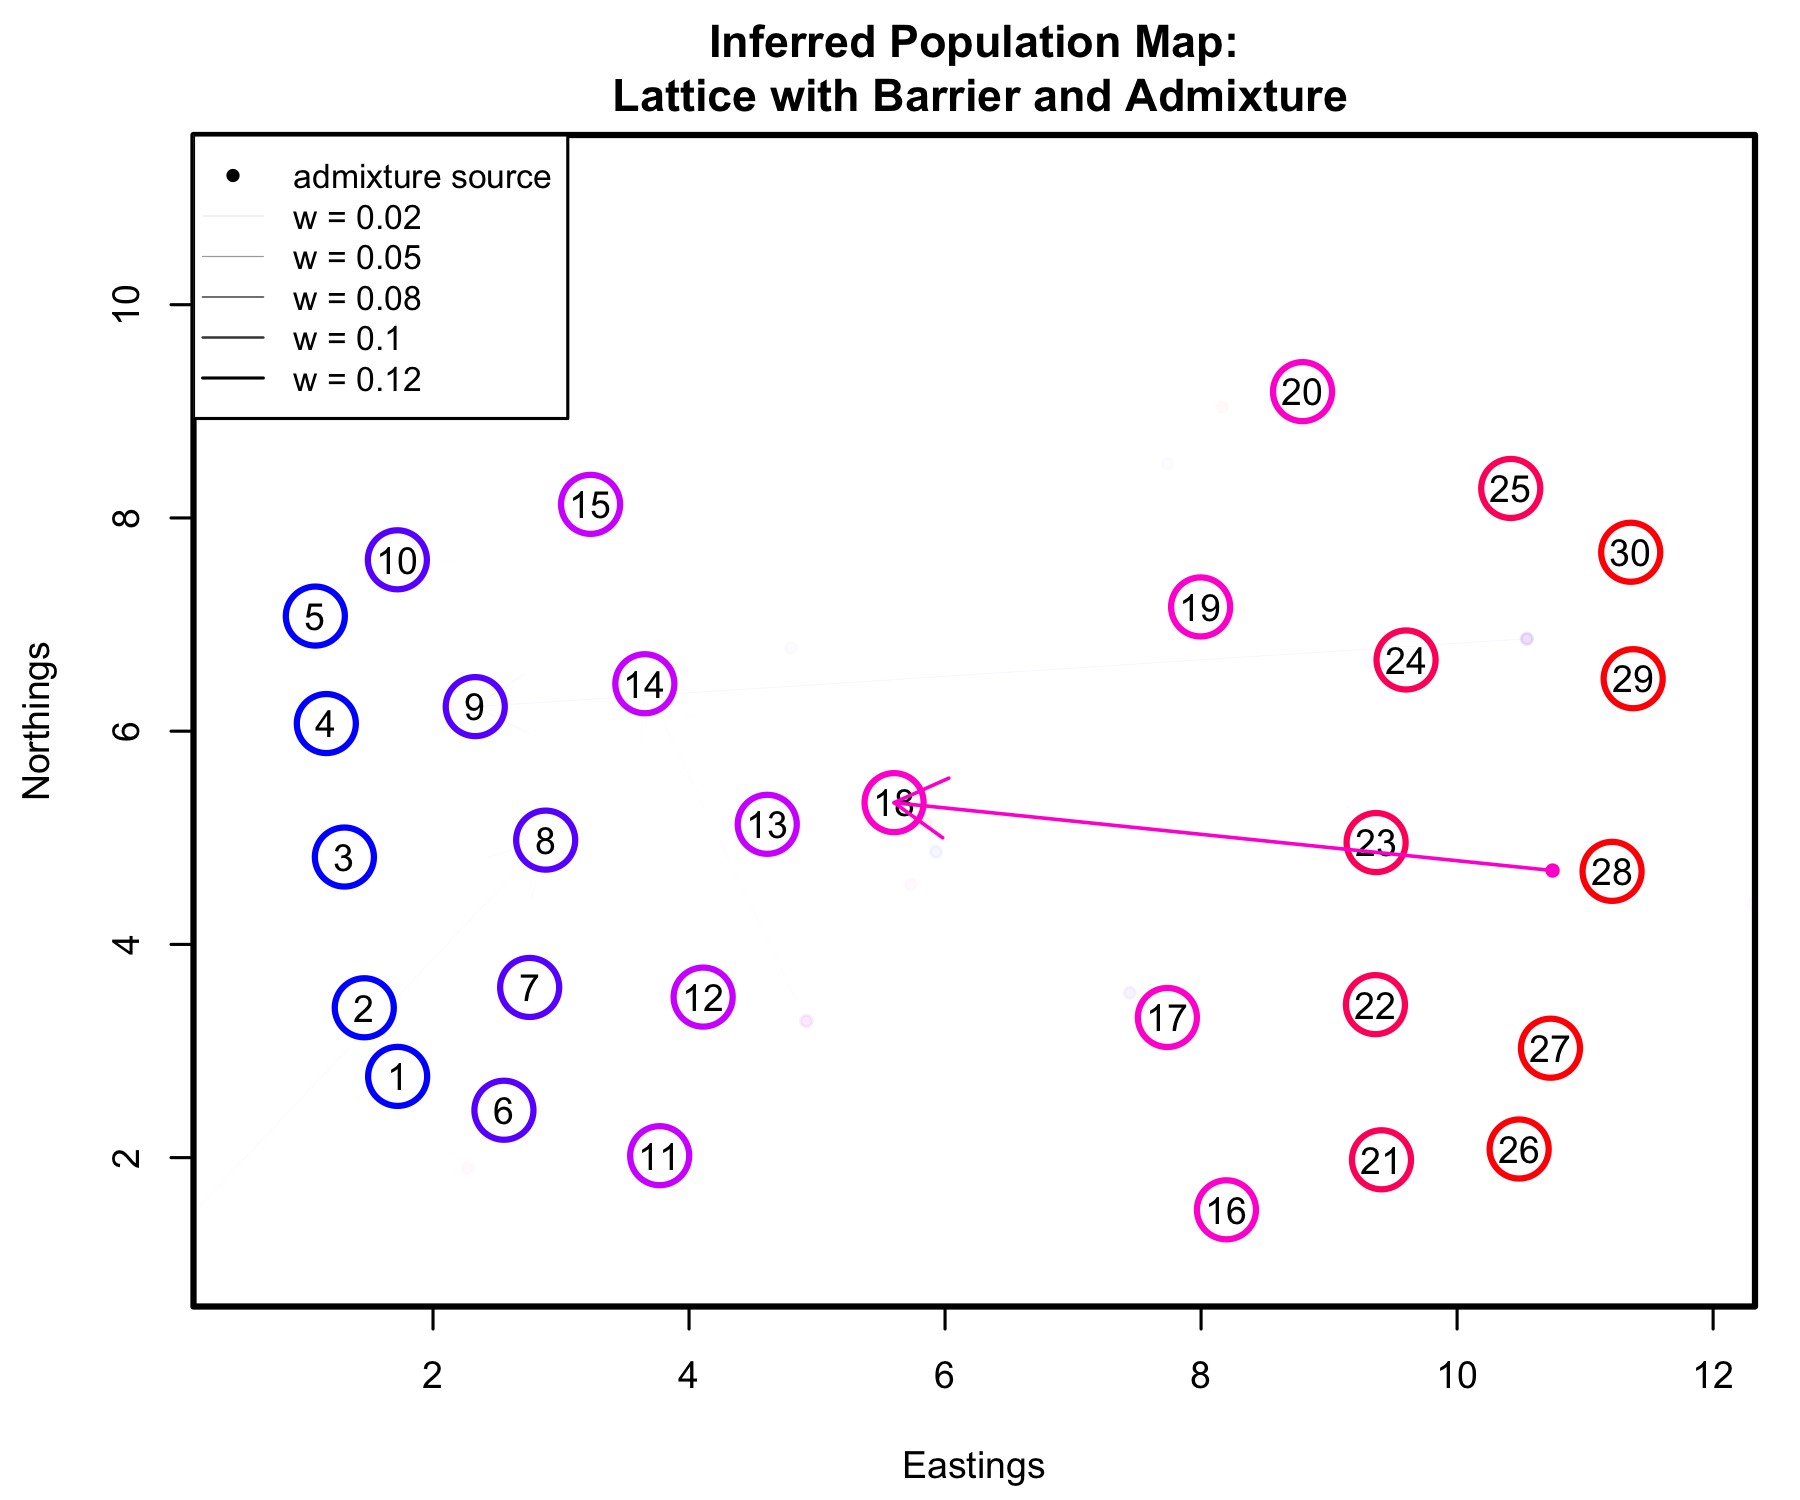
\includegraphics[width=2in,height=1.66in]{figs/sims/GeoGenMap_big_barr_ad_1.png}}
	\caption{Simulation scenarios and inferred population maps for two different admixture scenarios: a) lattice with a barrier and an admixture event across the barrier to an `inland' population; b) the inferred population map for the scenario in (a); c) lattice with a barrier and an admixture event across the barrier to a `neighbor' population on the border of the barrier; (d) the inferred population map for the scenario in (c).}\label{sfig:barr_inland_ad}
\end{figure}

\section*{Empirical Applications}
To demonstrate the applications of this novel method, we analyzed population genomic data from two systems: the greenish warbler ring species complex, and a global sampling of contemporary human populations.  Maps showing our sampling in these two systems are shown in Figure \ref{sfig:empirical_maps}, and information on the specific populations included is given in the Supplementary Materials, Tables \ref{tab:warbler_data_table} and \ref{tab:globe_data_table}.  To minimize the potential influence of the spatial prior on population locations, for each empirical analysis, we performed a SpaceMix run in which random, uniformly distributed locations between, for longitude, the minimum and maximum observed longitude, and, for latitude, the minimum and maximum observed latitude, were used as the prior on population locations (in addition to two runs for which the observed locations are used as priors).  For clarity and ease of interpretation, we then present a full Procrustes superimposition of the inferred population locations ($G'$) and their sources of admixture ($\identifyadmixsource{G}$), using the observed latitude and longitude of the populations/individuals ($G$) to give a reference position and orientation.  As results were generally consistent across multiple runs for each dataset regardless of the prior employed we (unless stated otherwise) present only the results from the `random' prior analyses.

\begin{figure}
	\centering
		\subcaptionbox{Warbler subspecies distribution map \label{irwin_map}}
			{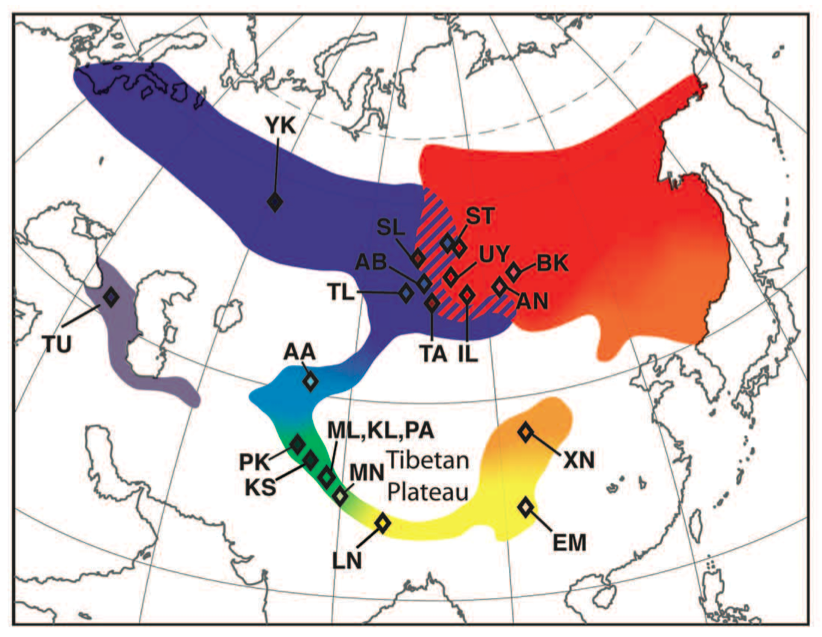
\includegraphics[width=2in,height=1.66in]{figs/warblers/Irwin_warbler_map_figure.png}}
		\subcaptionbox{Human sample distribution map \label{human_map}}
			{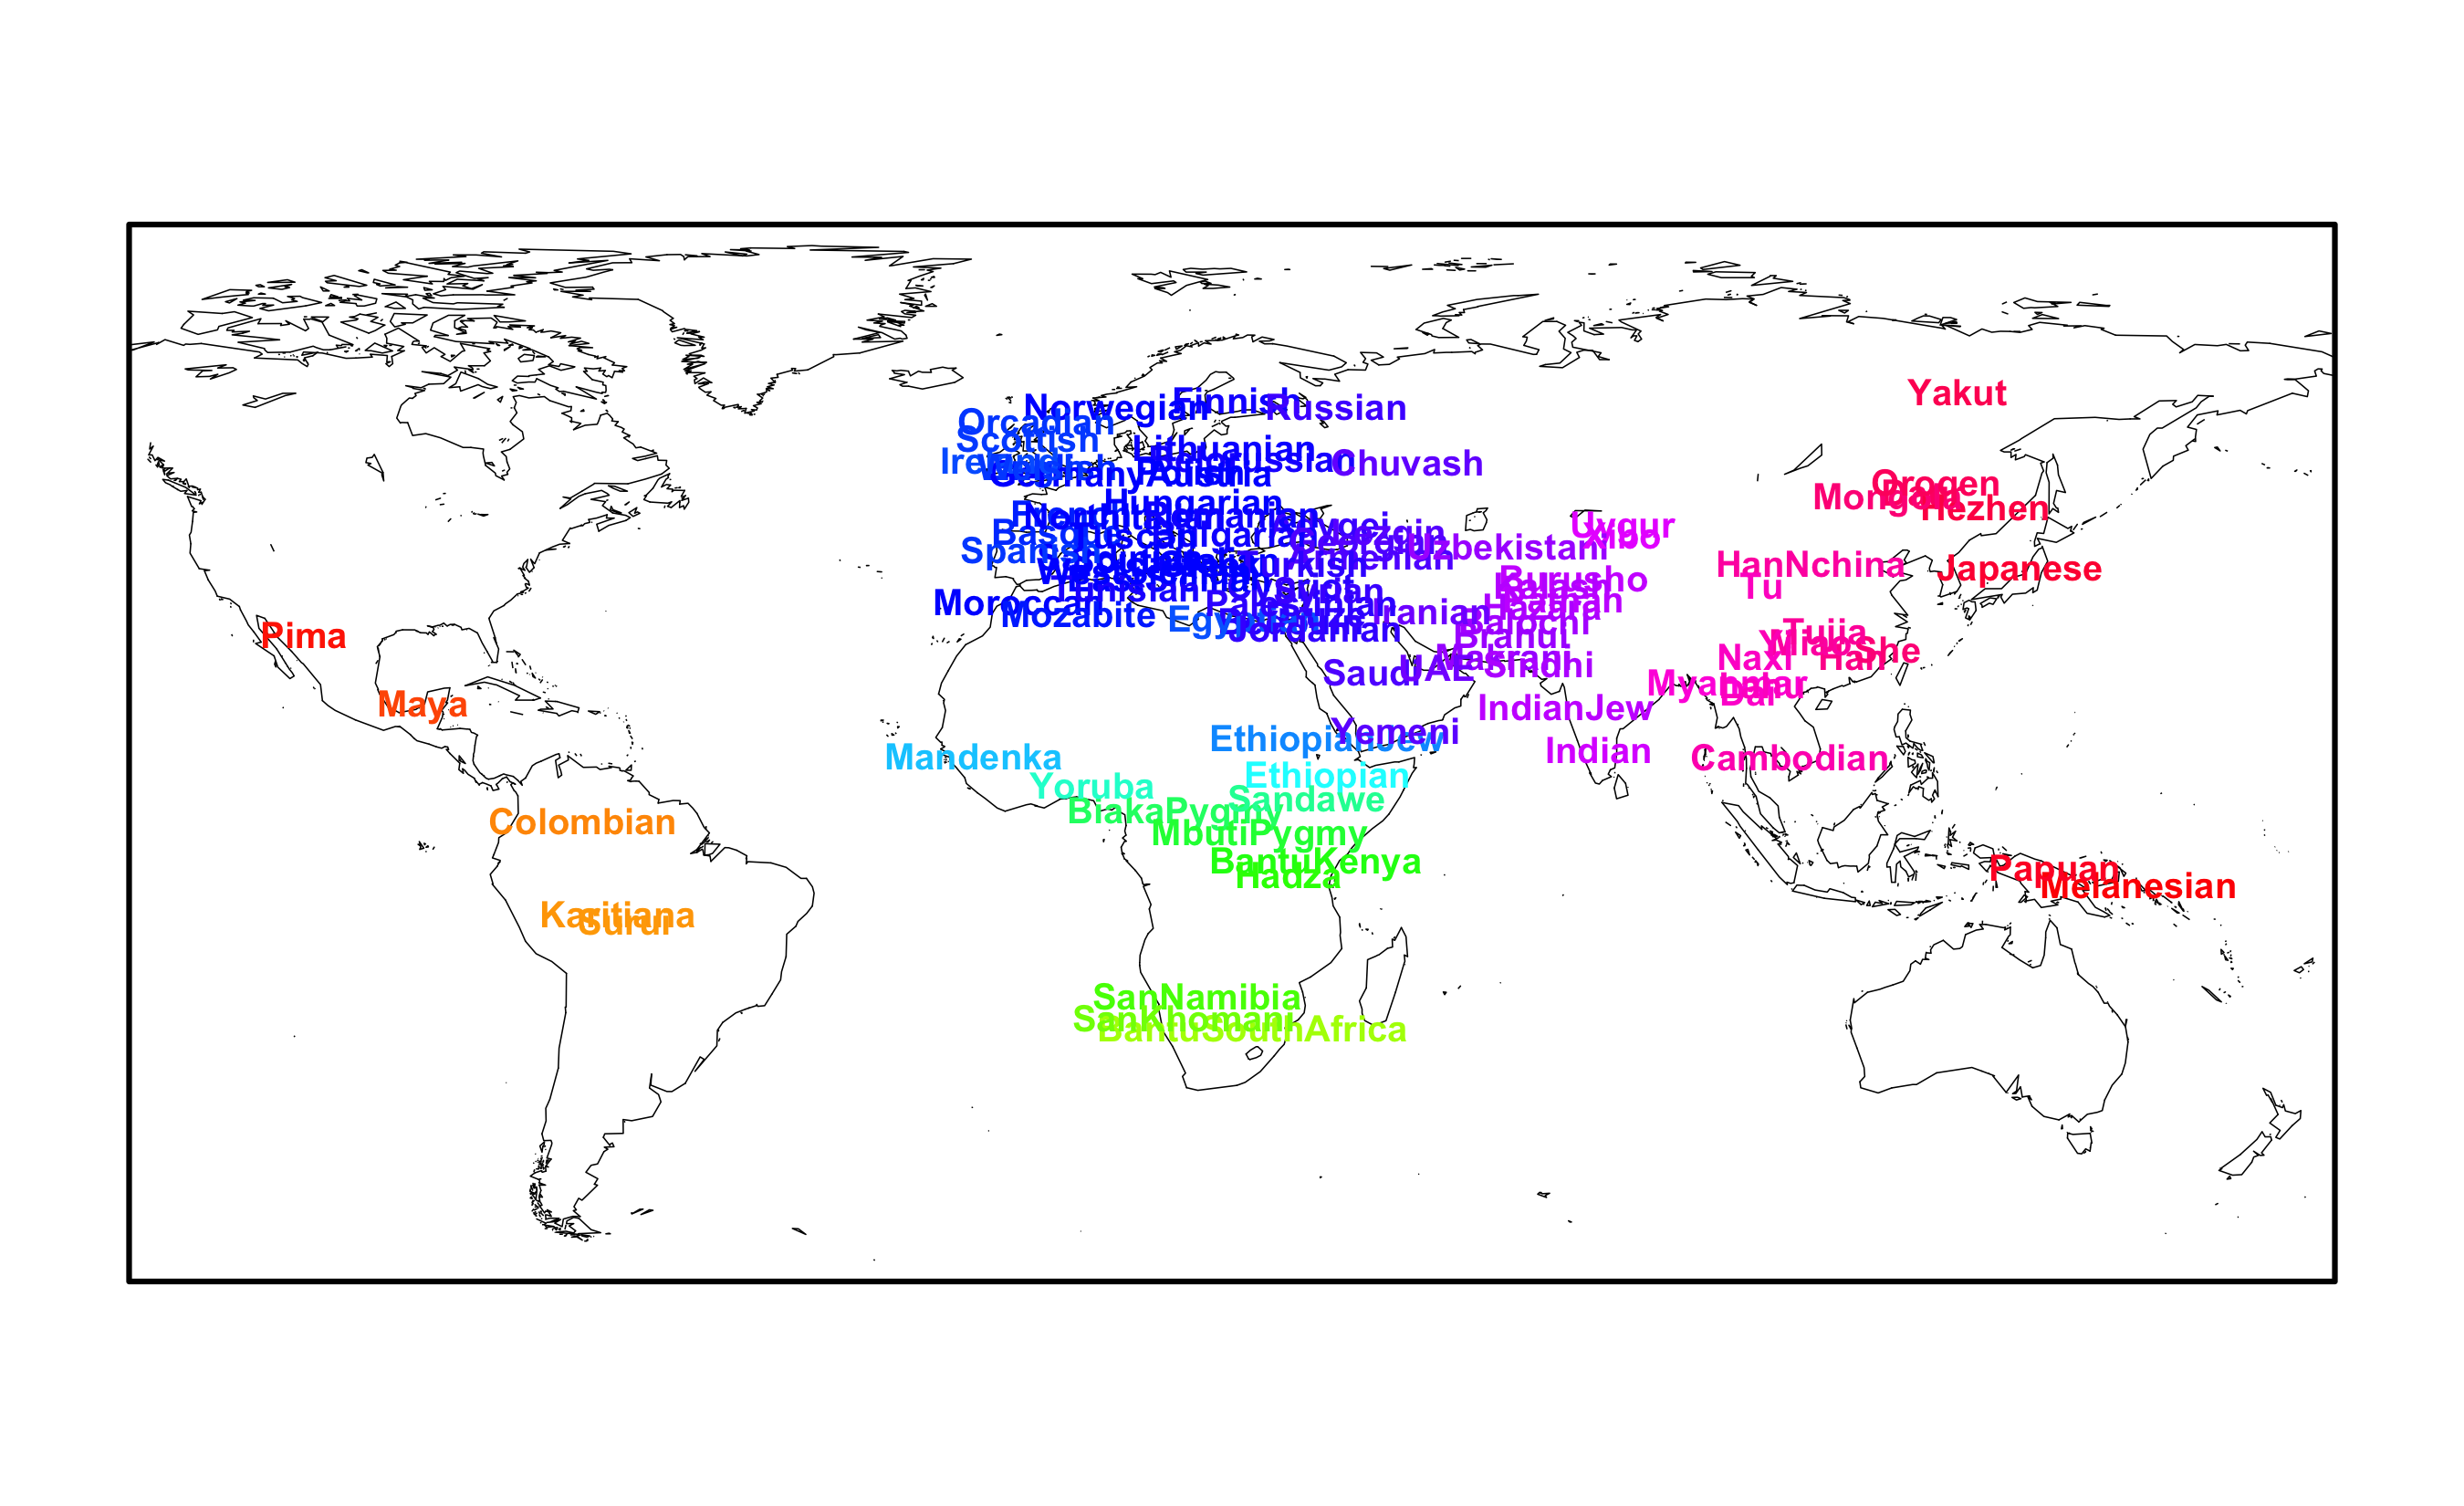
\includegraphics[width=4in,height=2.4in]{figs/globetrotter/globe_world_map_text.png}}
\caption{Sampling maps of both empirical systems analyzed.  (a) greenish warbler subspecies distributions of all 22 sampled populations, consisting of 95 individuals; (b) sampling map for human dataset, consisting of 1,490 individuals from 95 sampling locations.}
\label{sfig:empirical_maps}
\end{figure}

\subsection*{Greenish Warblers}  
The greenish warbler (\emph{Phylloscopus trochiloides}) species complex is broadly distributed around the Tibetan plateau, and exhibits gradients around the ring in a range of phenotypes including song, as well in allele frequencies (Ticehurst (1938), Irwin et al 2001, Irwin et al 2005, Irwin et al 2008).  At the northern end of the ring in central Siberia, where the eastern and western arms of population expansion meet, there are discontinuities in call and morphology, as well as reproductive isolation and a genetic discontinuity (Irwin et al 2001, Irwin et al 2008). It is proposed that the species complex represents a ring species, in which selection and/or drift, acting in the populations as they spread northward on either side of the Tibetan plateau, have led to the evolution of reproductive isolation between the terminal forms(REFs).  The question of whether it constitutes a ring species, in purest form, focuses on whether gene flow along the margins of the plateau has truly been continuous throughout the history of the expansion or if, alternatively, discontinuities in migration around the species complex's range have facilitated periods of differentiation in genotype or phenotype without gene flow (Mayr 1942, Mayr 1970, Coyne and Orr 2004).  However, we note that many would still classify this as a ring species even if that condition were not met, just not as a case of speciation-by-distance (see Wake and Schneider 1998 for discussion).

%Based on a larger SNP dataset, 
\citet{alcaide2014genomic} have suggested that the greenish warbler species complex constitutes a `broken' ring species, in which historical discontinuities in gene flow have facilitated the evolution of reproductive isolation between adjacent forms.  Because the questions in this system are fundamentally both geographic and genetic in nature, it is eminently SpaceMix-able, and, within this spatial framework, we performed a number of analyses to investigate the geographic context of population differentiation in the greenish warbler species complex. For these analyses, we used the dataset from \citet{alcaide2014genomic}, which consisted of 95 individuals sampled at 22 distinct locations and sequenced at 2,334 SNPs, of which 2,247 were bi-allelic and retained for SpaceMix runs.

\begin{figure}
	\centering
		\subcaptionbox{Warbler population map, no admixture \label{warb_pop_noad}}
			{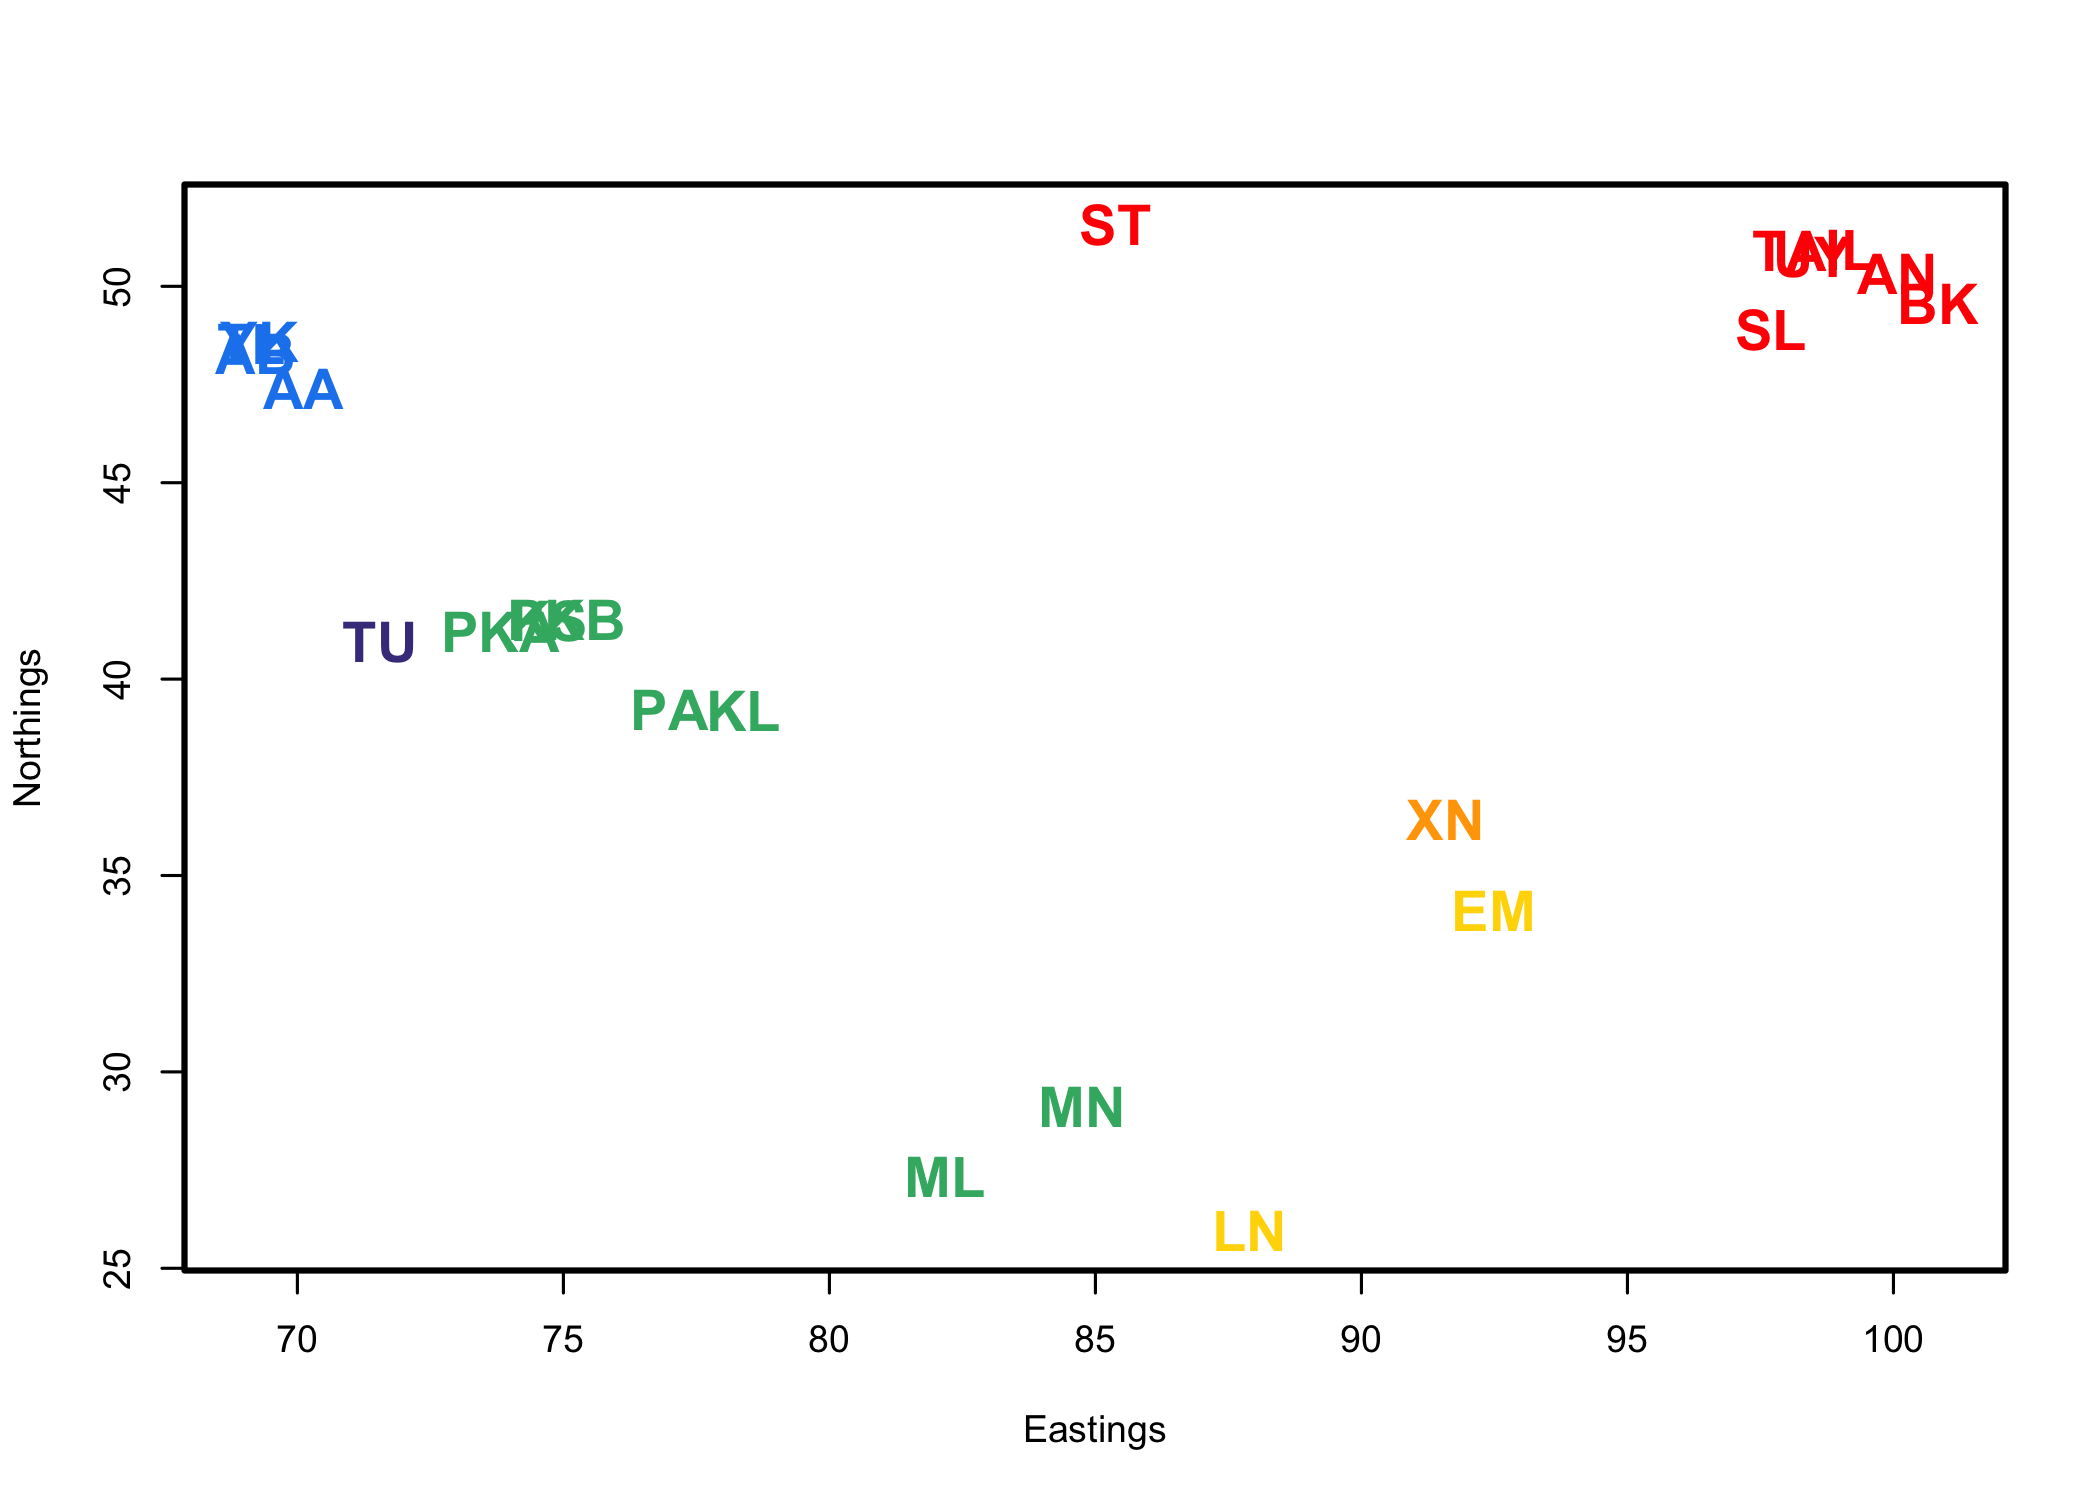
\includegraphics[width=2.4in,height=2in]{figs/warblers/warb_pop_noad.png}}
		\subcaptionbox{Warbler population map, with admixture \label{warb_pop_ad}}
			{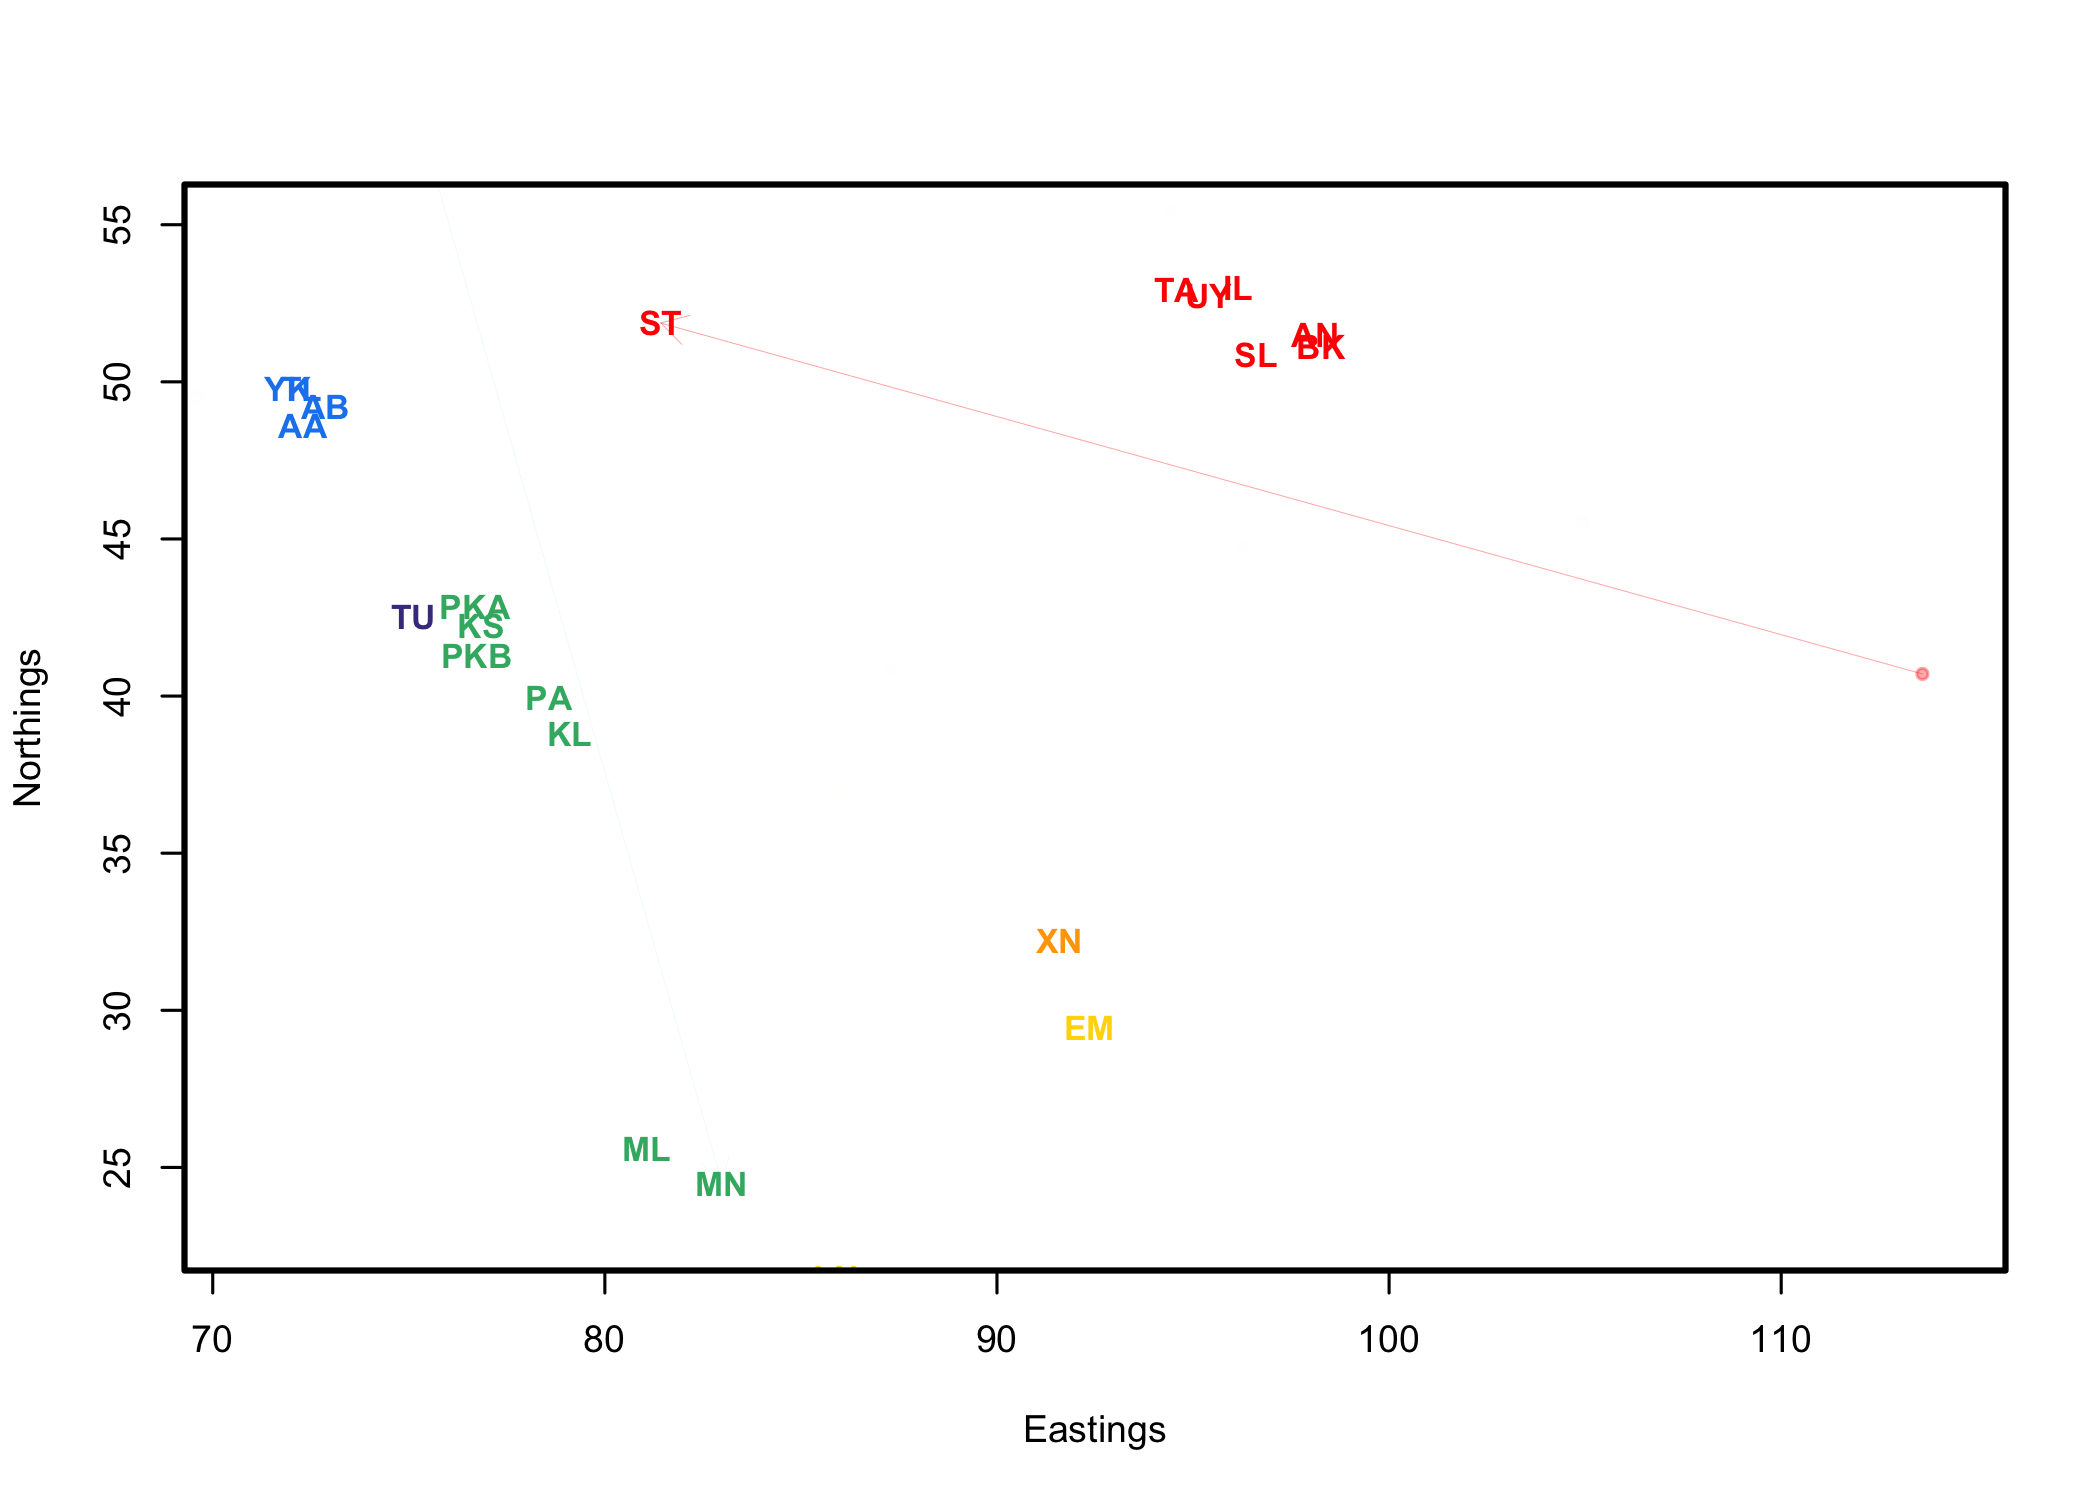
\includegraphics[width=2.4in,height=2in]{figs/warblers/population_warbler_map_randpr1.png}}
\caption{Inferred population maps with population labels colored as in \ref{sfig:empirical_maps}\subref{irwin_map}: a) the map inferred with no admixture inference; b) the map inferred with admixture inference.}
\label{sfig:warbler_pop}
\end{figure}

We first ran SpaceMix on the population dataset, with no admixture, setting the prior locations of the populations at random (as described above). The inferred map (Figure \ref{sfig:warbler_pop}\subref{warb_pop_noad}) largely recapitulates the geography of the sampled populations.  Populations choose locations around a large ring, with ordering similar to that of their true geographic locations.  The Turkish population (\textit{Phylloscopus trochiloides} ssp. \textit{nitidus}) clustered with the populations in the subspecies \textit{ludlowi}, but also chose a relatively high nugget parameter (see SuppMat Fig XXX), reflecting the independent drift it does not share with its \textit{ludlowi} neighbors.  The Yekat population of \textit{viridanus} individuals clusters closely with the other, less far-flung \textit{viridanus} individuals, indicating that differentiation within that subspecies is incommensurate with the amount of IBD expected for samples separated by that much distance. 

In the North, where the twin waves of expansion around the Tibetan Plateau are hypothesized to meet, the inferred geogenetic distance between populations identified as \textit{Phylloscopus trochiloides} ssp. \textit{plumbeitarsus} and ssp. \textit{viridanus} was much greater than their observed geographic separation, reflecting the reproductive isolation between these adjacent forms (see Figure \ref{sfig:warb_pop_distcomp}).  Interestingly, the ST population, which consists of six individuals sampled in Stolby, Russia, chooses a location intermediate between the \textit{plumbeitarsus} and \textit{viridanus} groups. The Stolby sample is composed of three individuals that belong to the eastern \textit{plumbeitarsus} and three individuals that belong to the western \textit{viridanus} \citep{alcaide2014genomic}. In the case where no admixture is allowed, this population is forced to adopt an intermediate position to incorporate its admixed nature.

%However, where the population-level analysis shows the Stolby population intermediate between the \textit{viridanus} and \textit{plumbeitarsus} clusters, the individual-level analysis reveals that the Stolby population (n=6)

We then ran the method allowing admixture, and again discuss the results from the analysis using random locations as priors on $G^{\prime}$ (Figure \ref{sfig:warbler_pop}\subref{warb_pop_ad}). The Stolby population chooses the highest admixture proportion, with a mean of 0.19 (95\% credible interval: 0.146-0.238).  Multiple runs agreed well on the level of admixture of the Stolby sample (see caption of Supplementary Figure \ref{sfig:warbler_pop_compare}). What does vary across runs is whether the Stolby population chooses to locate itself by the \textit{viridanus} cluster and draw admixture from near the \textit{plumbeitarsus}  cluster or vise versa; however, this is to be expected given the 50/50 nature of the sample's makeup (Supplementary Figure \ref{sfig:warbler_pop_compare}).

Because \textit{a priori} assigned population membership may be artificial (individuals from more than one population may be sampled at a single site), we repeated these analyses (with and without admixture) on an individual level (Figure \ref{sfig:warbler_ind_maps}).  In these analyses, the sample size in each `population' was 2 (for the two haplotypes in a diploid), and each individual chose its own location as well as the location of its source of admixture, the proportion of that admixture, and its nugget.  Because the analyses with and without admixture were nearly identical (individuals in the admixture analysis choose very low levels of admixture (see SuppMat Figure NNN); the population with the highest admixture proportion draws has a mean of 0.012 ($1.46 \times 10^{-4}$ to $4.73 \times 10^{-2}$)), we discuss the analysis with admixture inference.  As with the analysis on multi-sample populations, the results approximately mirror the geography of the individuals.

%The order of individuals' estimated locations around the Plateau is largely concordant with their true locations, and, in most cases, individuals sampled from the same population cluster closely together, as would be expected if samples collected at a single site are draws from a population that is locally panmictic.  
%\gb{could drop panels (A) and (B)}
\begin{figure}
	\centering
		\subcaptionbox{Warbler individuals map, no admixture \label{warb_ind_noad}}
			{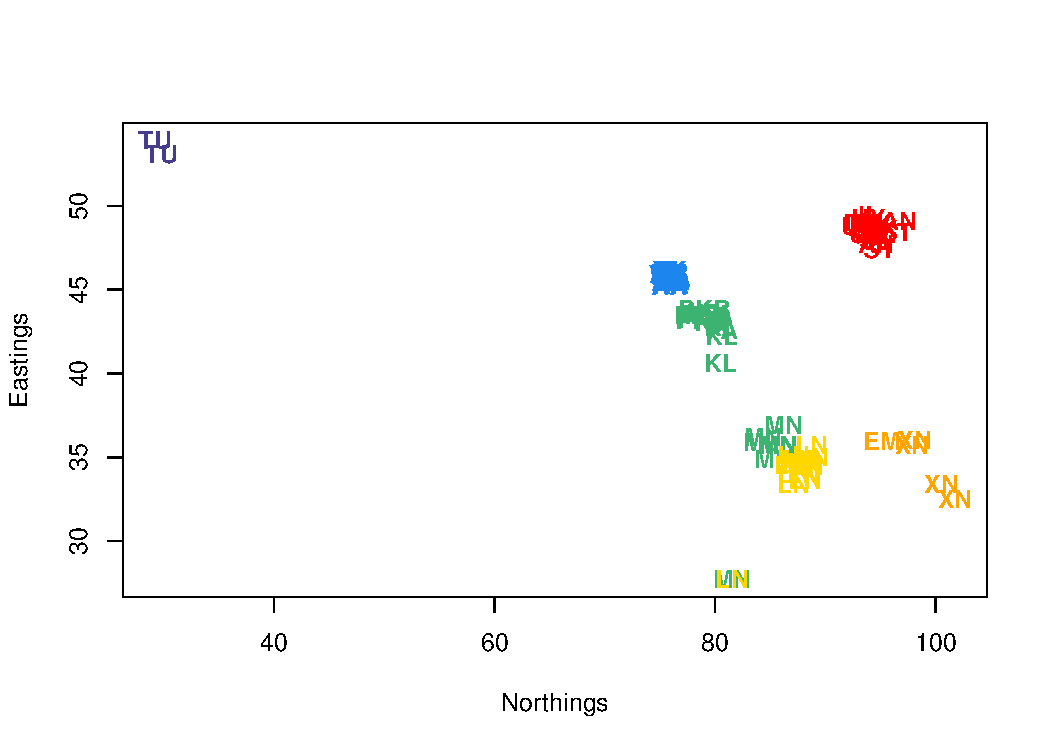
\includegraphics[width=2.8in,height=2.3in]{figs/warblers/warb_ind_noad.pdf}}
		\subcaptionbox{Closeup of non-\textit{nitidus} samples \label{warb_ind_noad_closeup}}
			{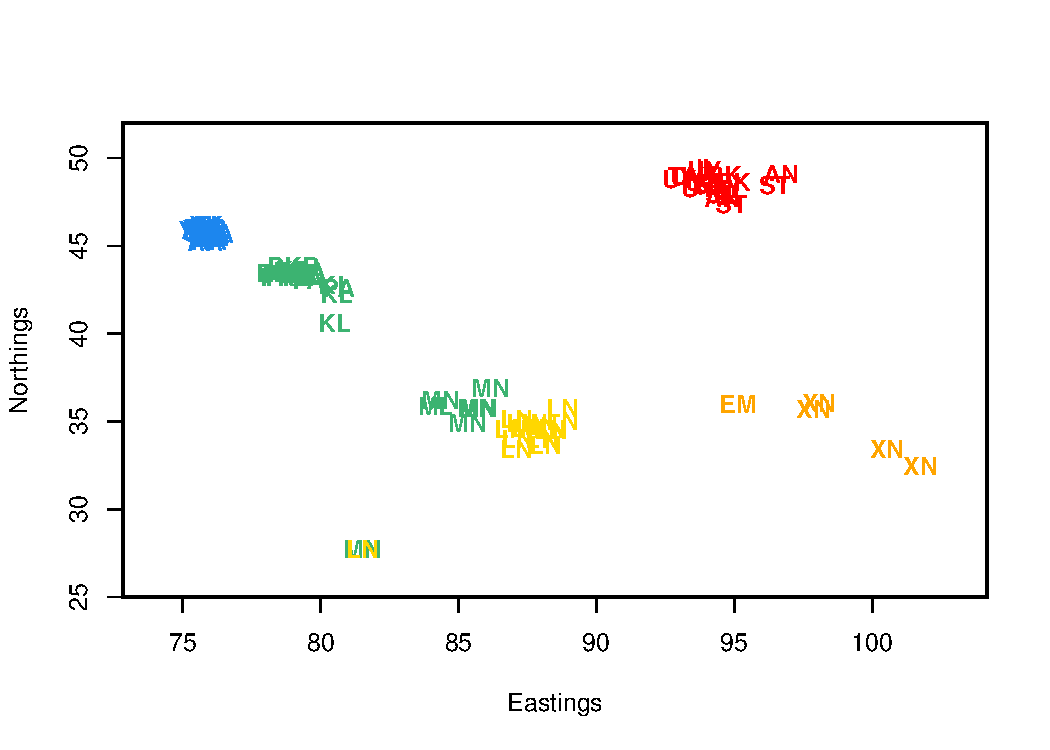
\includegraphics[width=2.8in,height=2.3in]{figs/warblers/warb_ind_noad_closeup.pdf}}
		\subcaptionbox{Warbler individuals map, admixture \label{warb_ind_ad}}
			{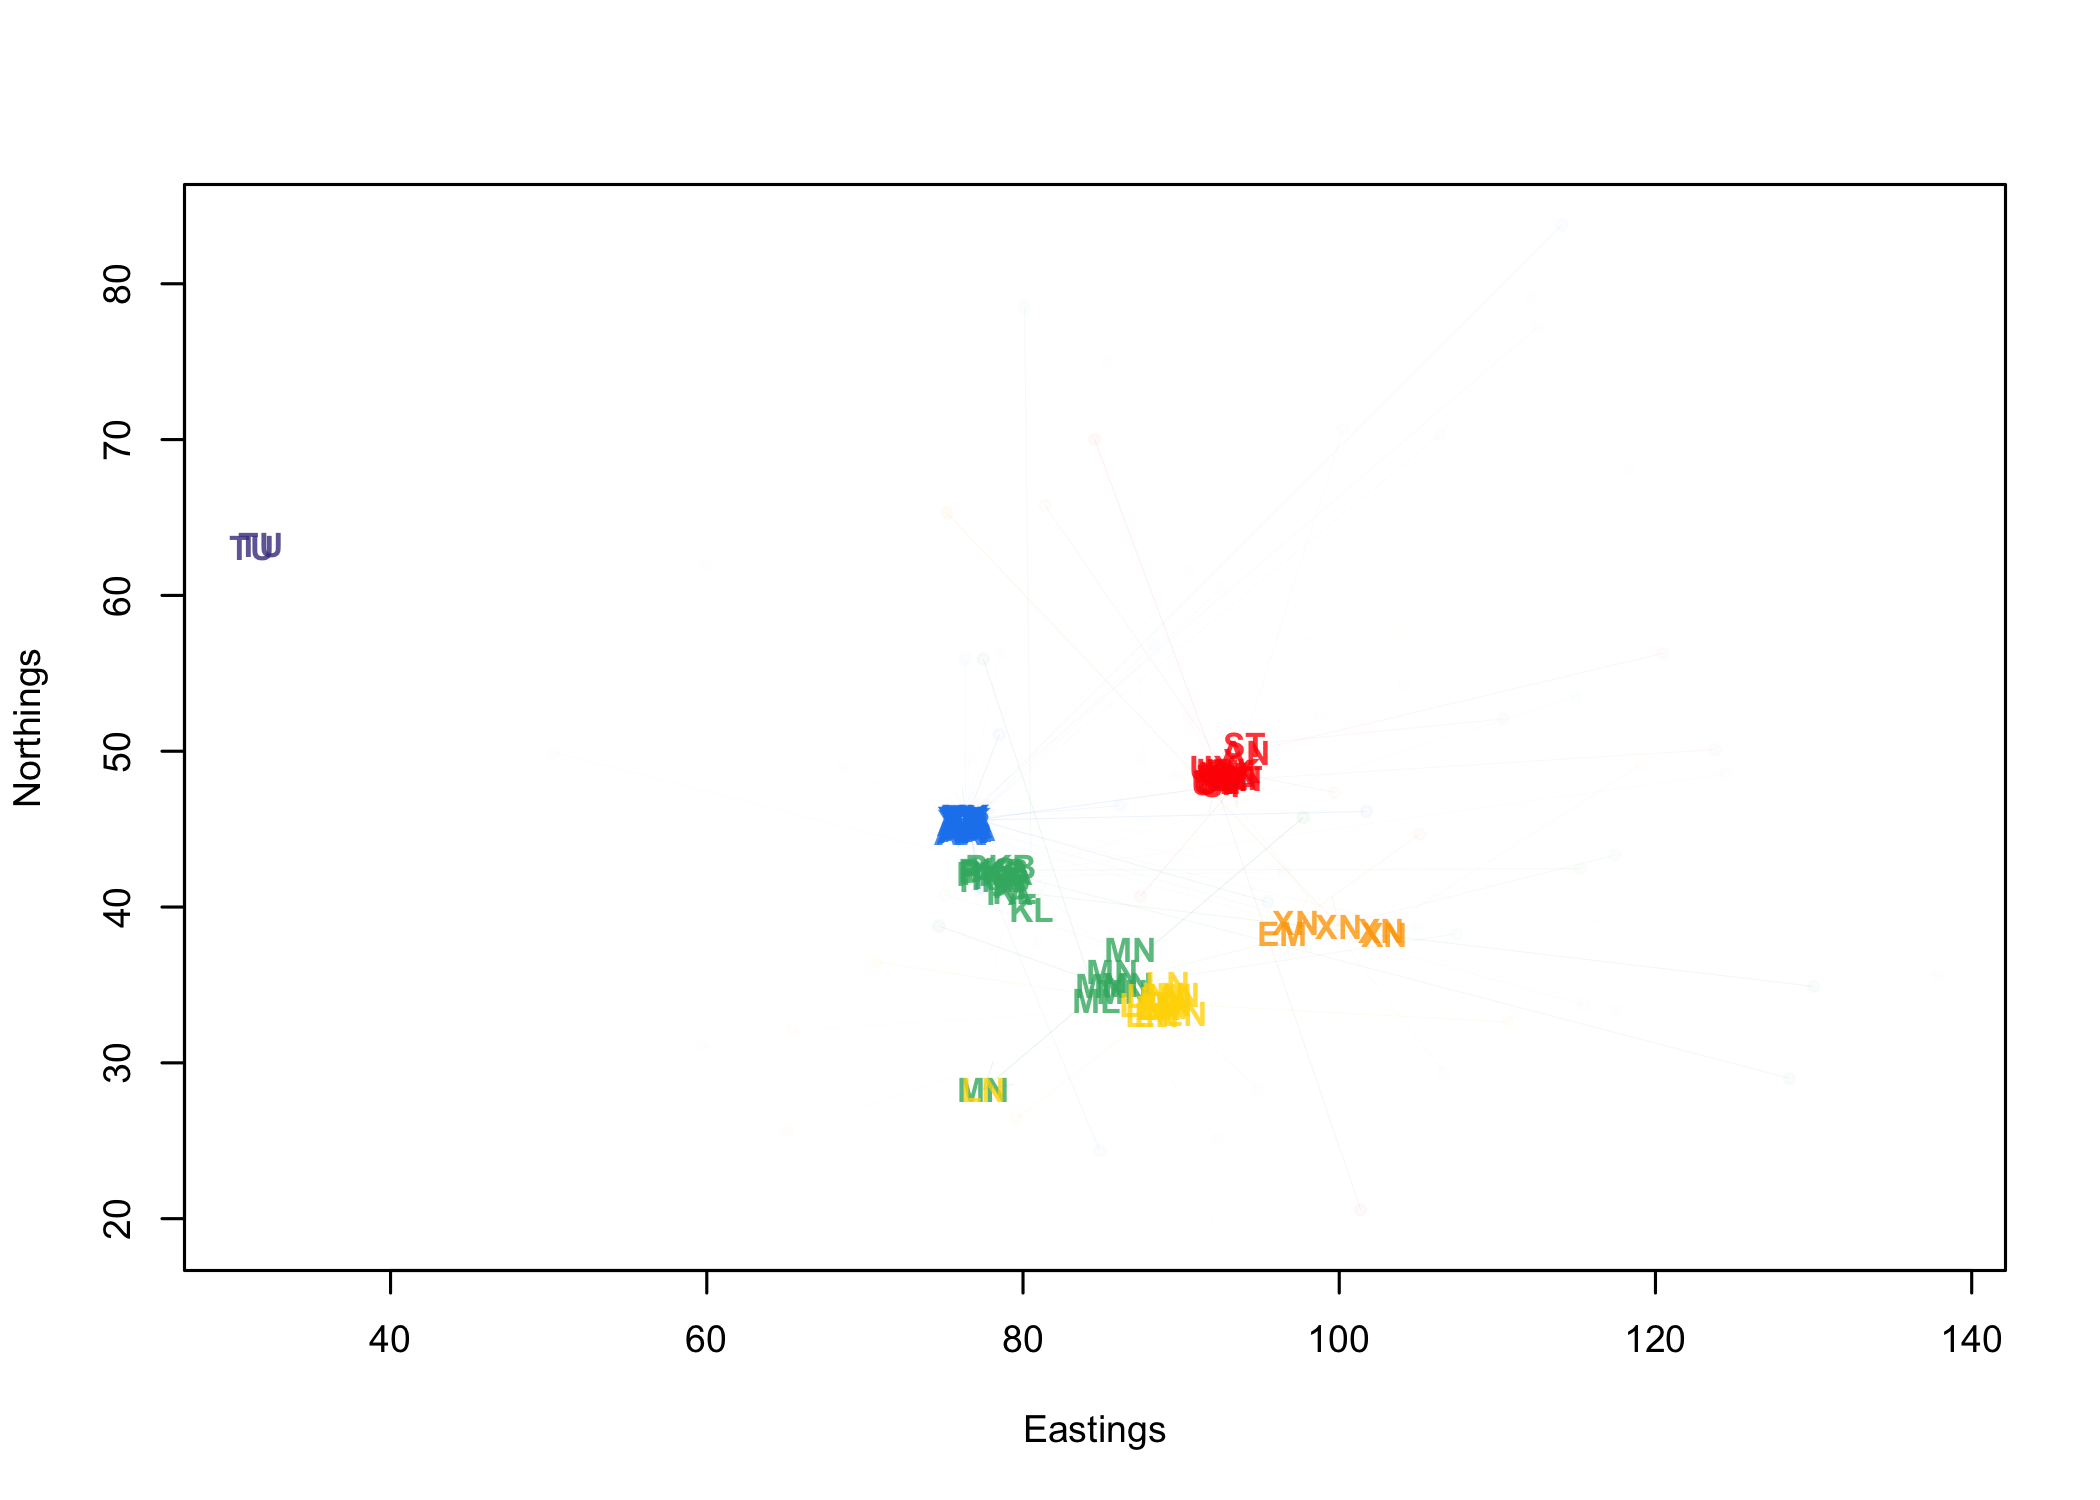
\includegraphics[width=2.8in,height=2.3in]{figs/warblers/individual_warbler_map_arrows_randpr1.png}}
		\subcaptionbox{Closeup of non-\textit{nitidus} samples \label{warb_ind_ad_closeup}}
			{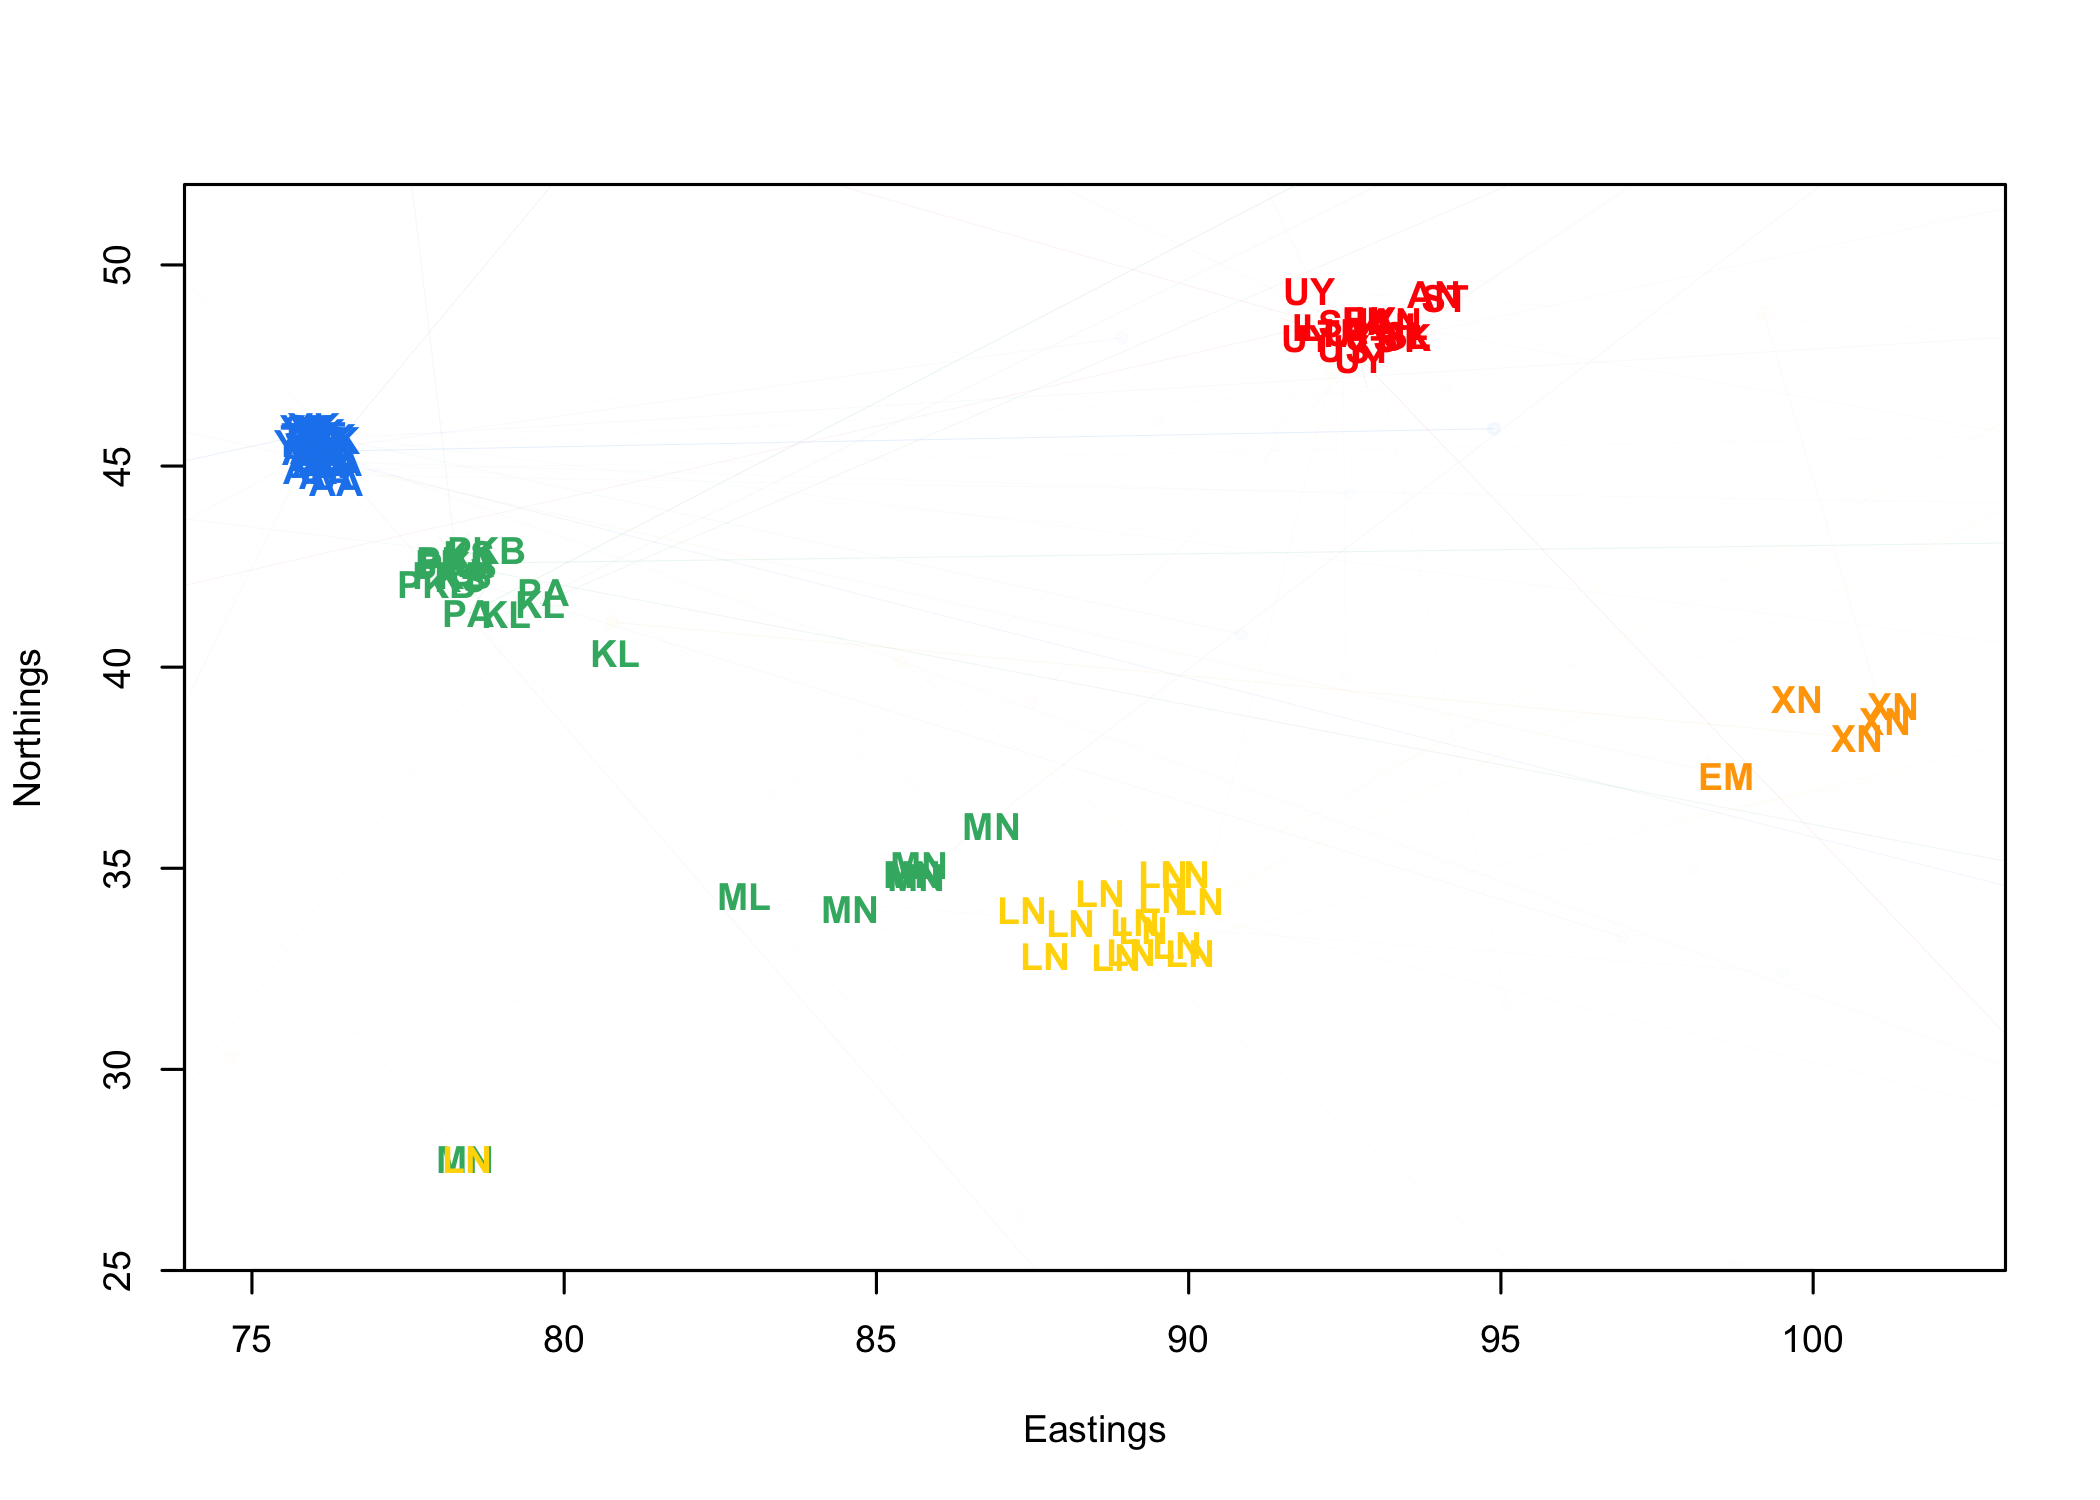
\includegraphics[width=2.8in,height=2.3in]{figs/warblers/individual_warbler_map_arrows_randpr1_closeup.png}}
	\caption{Inferred maps for warbler individuals, colored by subspecies under analyses with and without admixture inference. a) map inferred without admixture; (b) close up of all non-\textit{nitidus} samples in non-admixture map; c) map inferred with admixture; d) closeup of all non-\textit{nitrides} samples in the admixture map.}\label{sfig:warbler_ind_maps}
\end{figure}

There are, however, a number of obvious departures in the individual inferred geogenetic map from the observed map. The most obvious again is the clear split between \textit{viridanus} and \textit{plumbeitarsus} individuals in the north at the contact zone of the two waves of expansion.  This is clearer now than in the population-based analysis as individuals from the Stolby population have moved to near their respective \textit{viridanus} and \textit{plumbeitarsus} clusters. 

Despite the fact that \textit{viridanus} and \textit{plumbeitarsus} individuals have moved away from each other in our geogenetic map, they are still closer to each other than we might expect if their drift were truly independent (e.g.\ our populations could form along a line, with \textit{viridanus} at one end and \textit{plumbeitarsus} at the other). This horseshoe, with \textit{viridanus} and \textit{plumbeitarsus} at its tips, is steady within and among runs of the MCMC and choice of position priors (see Supplementary clouds NNN).  

Is this biologically meaningful?  A similar horseshoe shape appears when a principal components (PC) analysis is conducted and individuals are plotted on the first two PCs \citep[][see SuppMat Figure \ref{sfig:warb_ind_PC_map}]{alcaide2014genomic}.  However, as discussed by Novembre \& Stephens (2008) such patterns in PC analysis can arise for somewhat unintuitive reasons. If populations are simulated under a one dimensional stepping stone model, then plotting individuals on the first two PCs results in a horseshoe (e.g.\ see SuppMat Figure \ref{sfig:line_scenario}\subref{line_pops_pca}) not because of gene flow connecting between the tips, but rather because of the orthogonality requirement of PCs (see Novembre \& Stephens for more discussion).  In contrast, when SpaceMix is applied to one dimensional stepping stone data, the placement of samples is consistent with a line (see SuppMat Figures \ref{sfig:line_scenario}\subref{line_pops_post}, \ref{sfig:line_scenario}\subref{line_pops_MAP}).

In addition, when we run SpaceMix on the greenish warbler individuals, specifying their location priors to fall along a straight line with samples located at their approximate positions around the horseshoe, the posterior positions of the populations still curl up to form a rough horseshoe (SuppMat Figure \ref{sfig:warb_inds_on_a_line}). The proximity of \textit{viridanus} and \textit{plumbeitarsus} in geogenetic space may be due to gene flow between the tips of the horseshoe north of the Tibetan Plateau. This conclusion is in agreement with that of \citet{alcaide2014genomic}, who observed evidence of hybridization between \textit{viridanus} and \textit{plumbeitarsus} using assignment methods.

A second difference between the observed and inferred maps is a pair of individuals, one identified as \textit{P. t. ludlowi} (Lud-MN3), one as \textit{P. t. trochiloides} (Tro-LN11), that choose locations very close to one another and also away from the other individuals sampled at their locations. Examining pairwise sequence divergence reveals that these two individuals show unusually recent common ancestry (see SuppMat Figure NNN), and therefore are likely expressing their shared ancestry (drift unshared with other \textit{ludlowi} and \textit{trochiloides} individuals) by choosing locations that are close to each other and far from their respective clusters of individuals that were sampled at the same sites.

The SpaceMix map also diverges from the observed map in the distribution of individuals from the subspecies \textit{ludlowi}.  These samples were taken from seven sampling locations along the southwest margin of the Tibetan Plateau, but, in the SpaceMix analysis, they partition into two main clusters, one near the \textit{trochiloides} cluster, and one near the \textit{viridanus} cluster.  This break between samples from the same subspecies, which is concordant with the findings of \citet{alcaide2014genomic}, makes the \textit{ludlowi} cluster unusual compared to the estimated spatial distributions of the other subspecies (see SuppMat Figure \ref{sfig:warb_ind_distcomp}).

%
\subsection*{Human Populations}
The geography of human population structure is a complex product of the forces of migration, drift, and selection acting on both local and global scales.  Recent work in this area has demonstrated that the signature of these forces can be read in the genomes of modern humans (e.g.\ Novembre et al 2008, Ralph \& Coop 2013, Moorjani, Reich, ARG folks, Hellenthal et al 2014).  This research has revealed that patterns of spatial genetic differentiation across human populations are byzantine in their complexity, varying across both space (Ralph \& Coop 2013) and time (Skoglund et al 2012, 2014), and shaped by culture (Reich et al 2009, Atzmon et al 2010, Moorjani et al 2011), landscape (Bradburd, Ralph, Coop 2013), and environment (Beall et al 2010, Bigham et al 2010).  

To visualize the patterns these processes have induced, we create a geogenetic map for a worldwide sample of modern human populations. In doing so we fully acknowledge that human history at these geographic scales has many aspects that are not well captured by isolation distance or simple admixture models. To simplify the discussion of our results, we talk about samples' locations and those of their sources of admixture, but of course both reflect the compounding of drift and gene flow over many historical processes.  We therefore urge caution in the interpretation our results, and view them as an overly simplistic but rich visualization of patterns of population structure in humans.


% Specifically, our research questions were: 
% \begin{enumerate}
% \item What is the geography of human population structure?  Which populations cluster with which, and how does the geogenetic map contrast with the observed geography?
% \item Can the map we estimate reconstruct the many of the important expansion events in human pre-history, including the out-of-Africa expansion, the colonizations of Oceania, and the colonization of the Americas via Beringia?
% \item Which human populations are most greatly admixed, and from where?  Will the SpaceMix results confirm the admixture findings of previous studies?
% \end{enumerate}

%To answer these questions,

We used a random subset of 10,000 SNPs from the SNP dataset of Hellenthal et al (2014), which is comprised of 1,490 sampled in 95 populations (see Fig. \ref{sfig:empirical_maps}\subref{human_map} for map of sampling), as well as the latitude and longitude attributed to each population.  We ran two sets of SpaceMix analyses: in the first, we estimated population locations, and in the second, we estimated population locations, as well as their admixture sources and amounts.

In the analysis in which populations choose their own locations, the map roughly recapitulates the geography of the samples (Fig. \ref{sfig:globe_noad_maps}).  Populations generally cluster with other populations sampled on their continent, and the relative placement of populations is similar to that of their observed geography.  Sub-Saharan African populations are distributed in a manner consistent with their sampled latitude, with the San populations in the South and the Ethiopian populations closest to the Eurasian populations in the North.  North African populations, such as the Moroccan, Tunisian, and Egyptian populations, cluster with Middle Eastern populations such as the Yemeni and the UAE, and are quite close to both the Ethiopian populations and the western European populations, such as the Sicilians, the Cypriots, the Tuscans, and the Sardinians.

Within Eurasia, we see populations grouping roughly in the order of their longitude on the continent, with British, continental European, and Russian populations at the western margin, and Han, Japanese, and Southeast Asian populations such as the Cambodians, the Lahu, and Myanmar on the eastern margin.  Interspersed between are populations of the Sub-continent, such as the Indian, Indian Jewish, and Sindhi populations, as well as populations from farther north in Eurasia that choose intermediate locations between European and East Asian populations, such as the Uygur, the Hazara, the Uzbekistani, and the Chuvash.  Populations from the Americas cluster together and choose a location close to the East Asian populations, as do the populations from Oceania.

\begin{figure}
	\centering
		\subcaptionbox{Inferred map of human populations \label{globe_all_noad_map}}
			{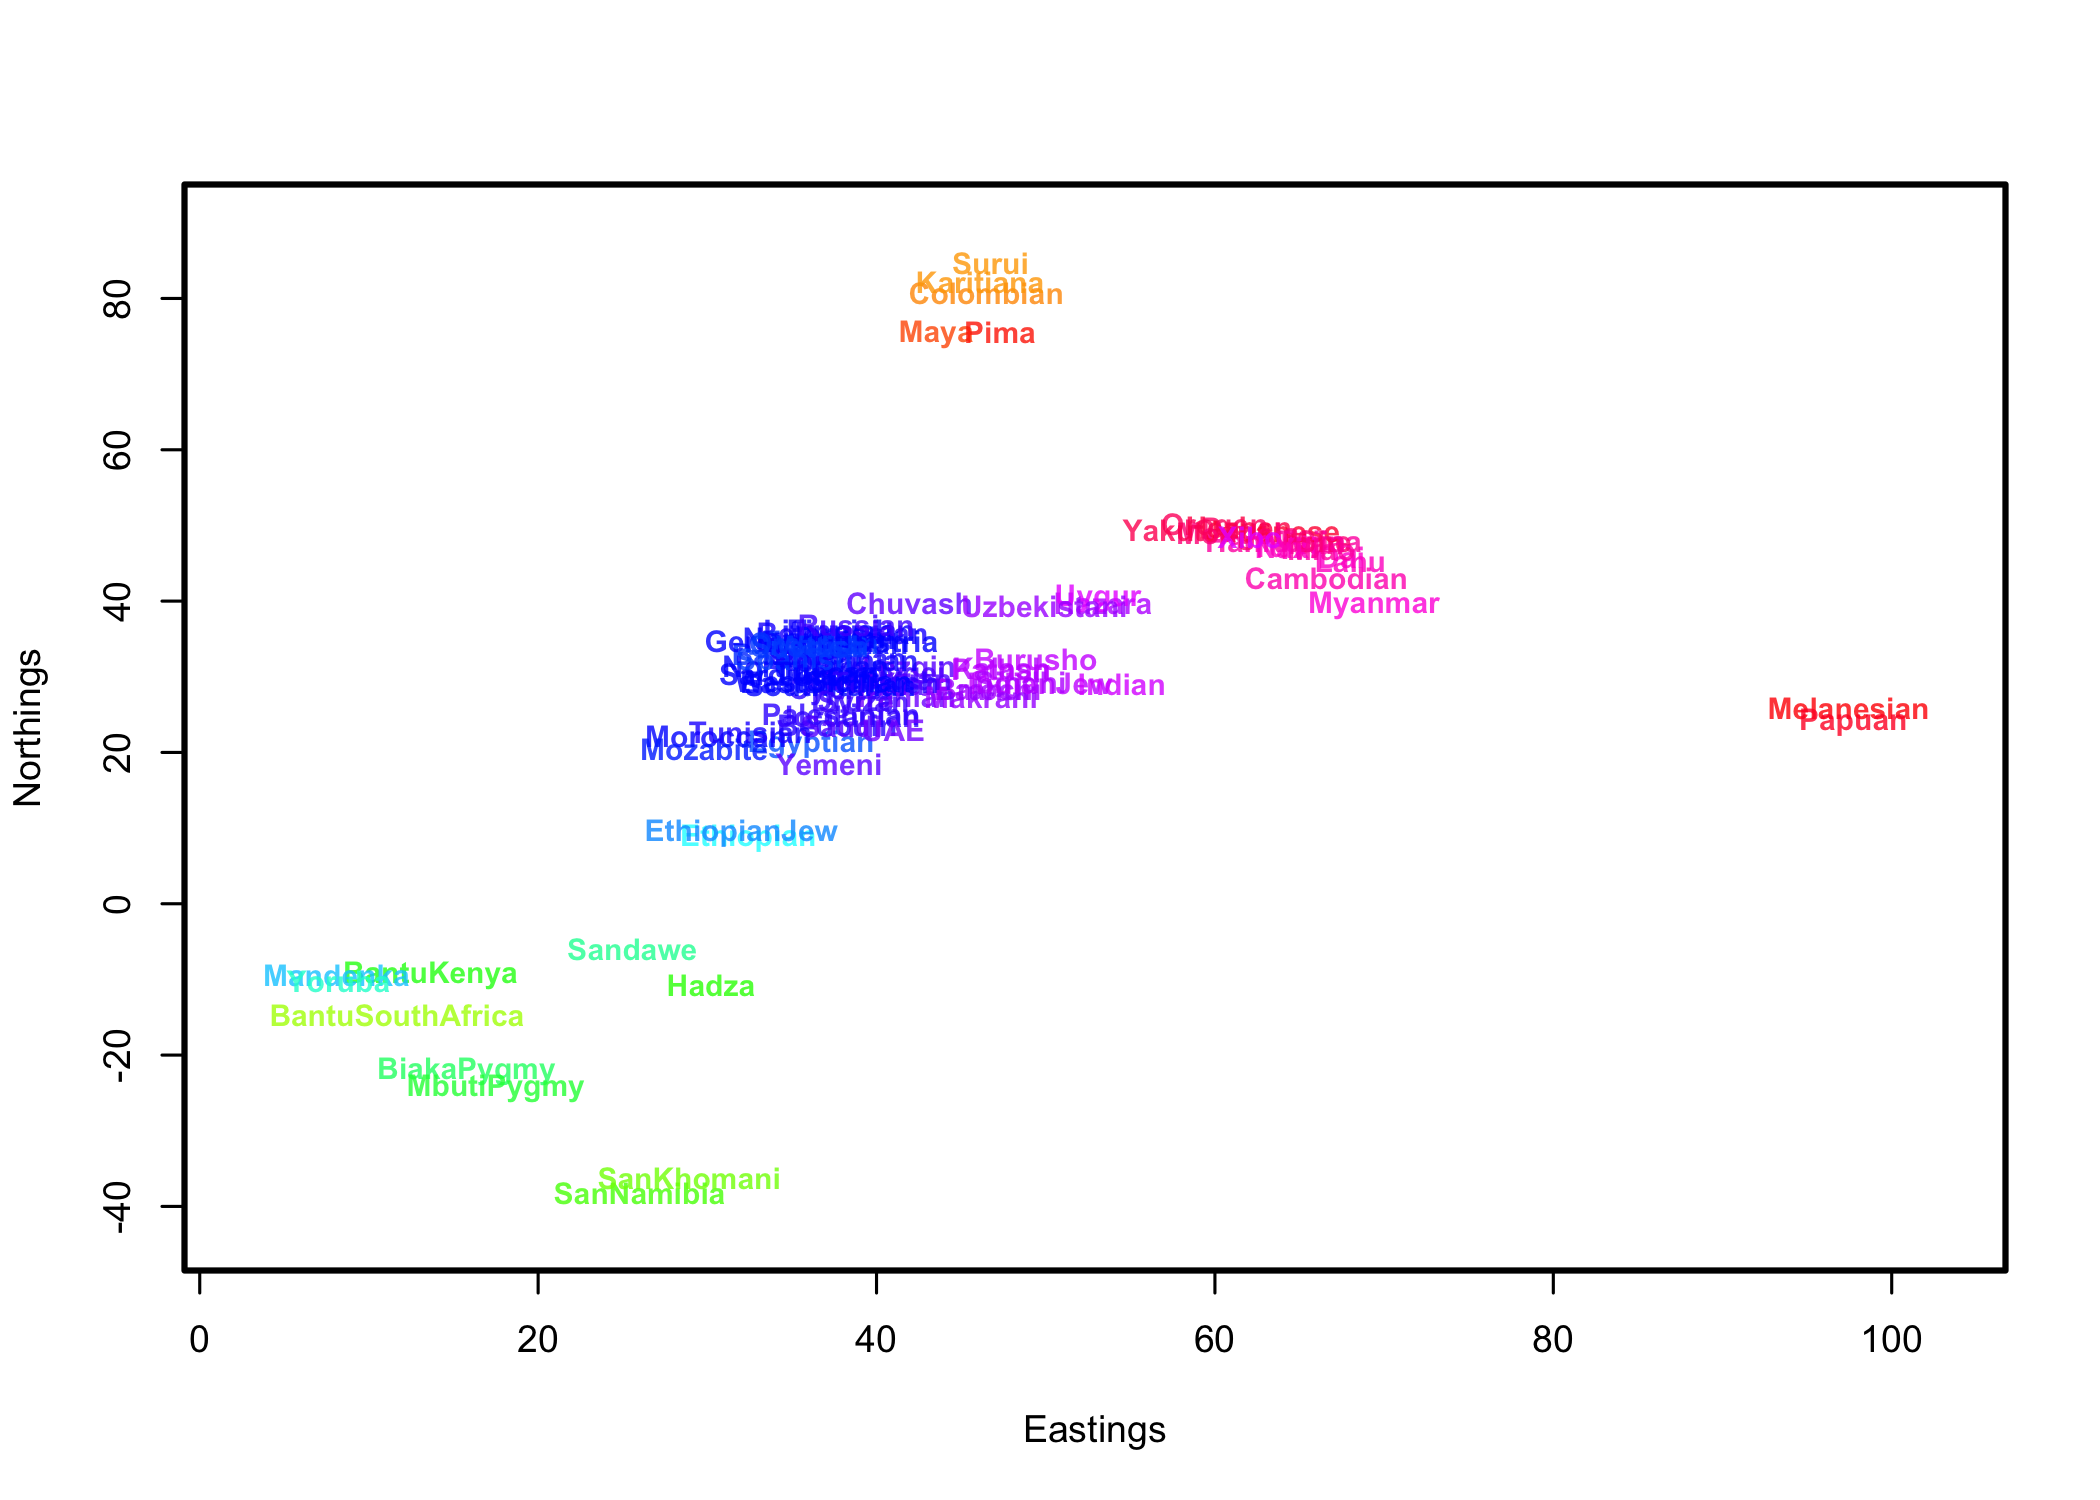
\includegraphics[width=2.8in,height=2.3in]{figs/globetrotter/globe_NoAd_map.png}}
		\subcaptionbox{Closeup of Eurasian populations \label{globe_eurasia_noad_map}}
			{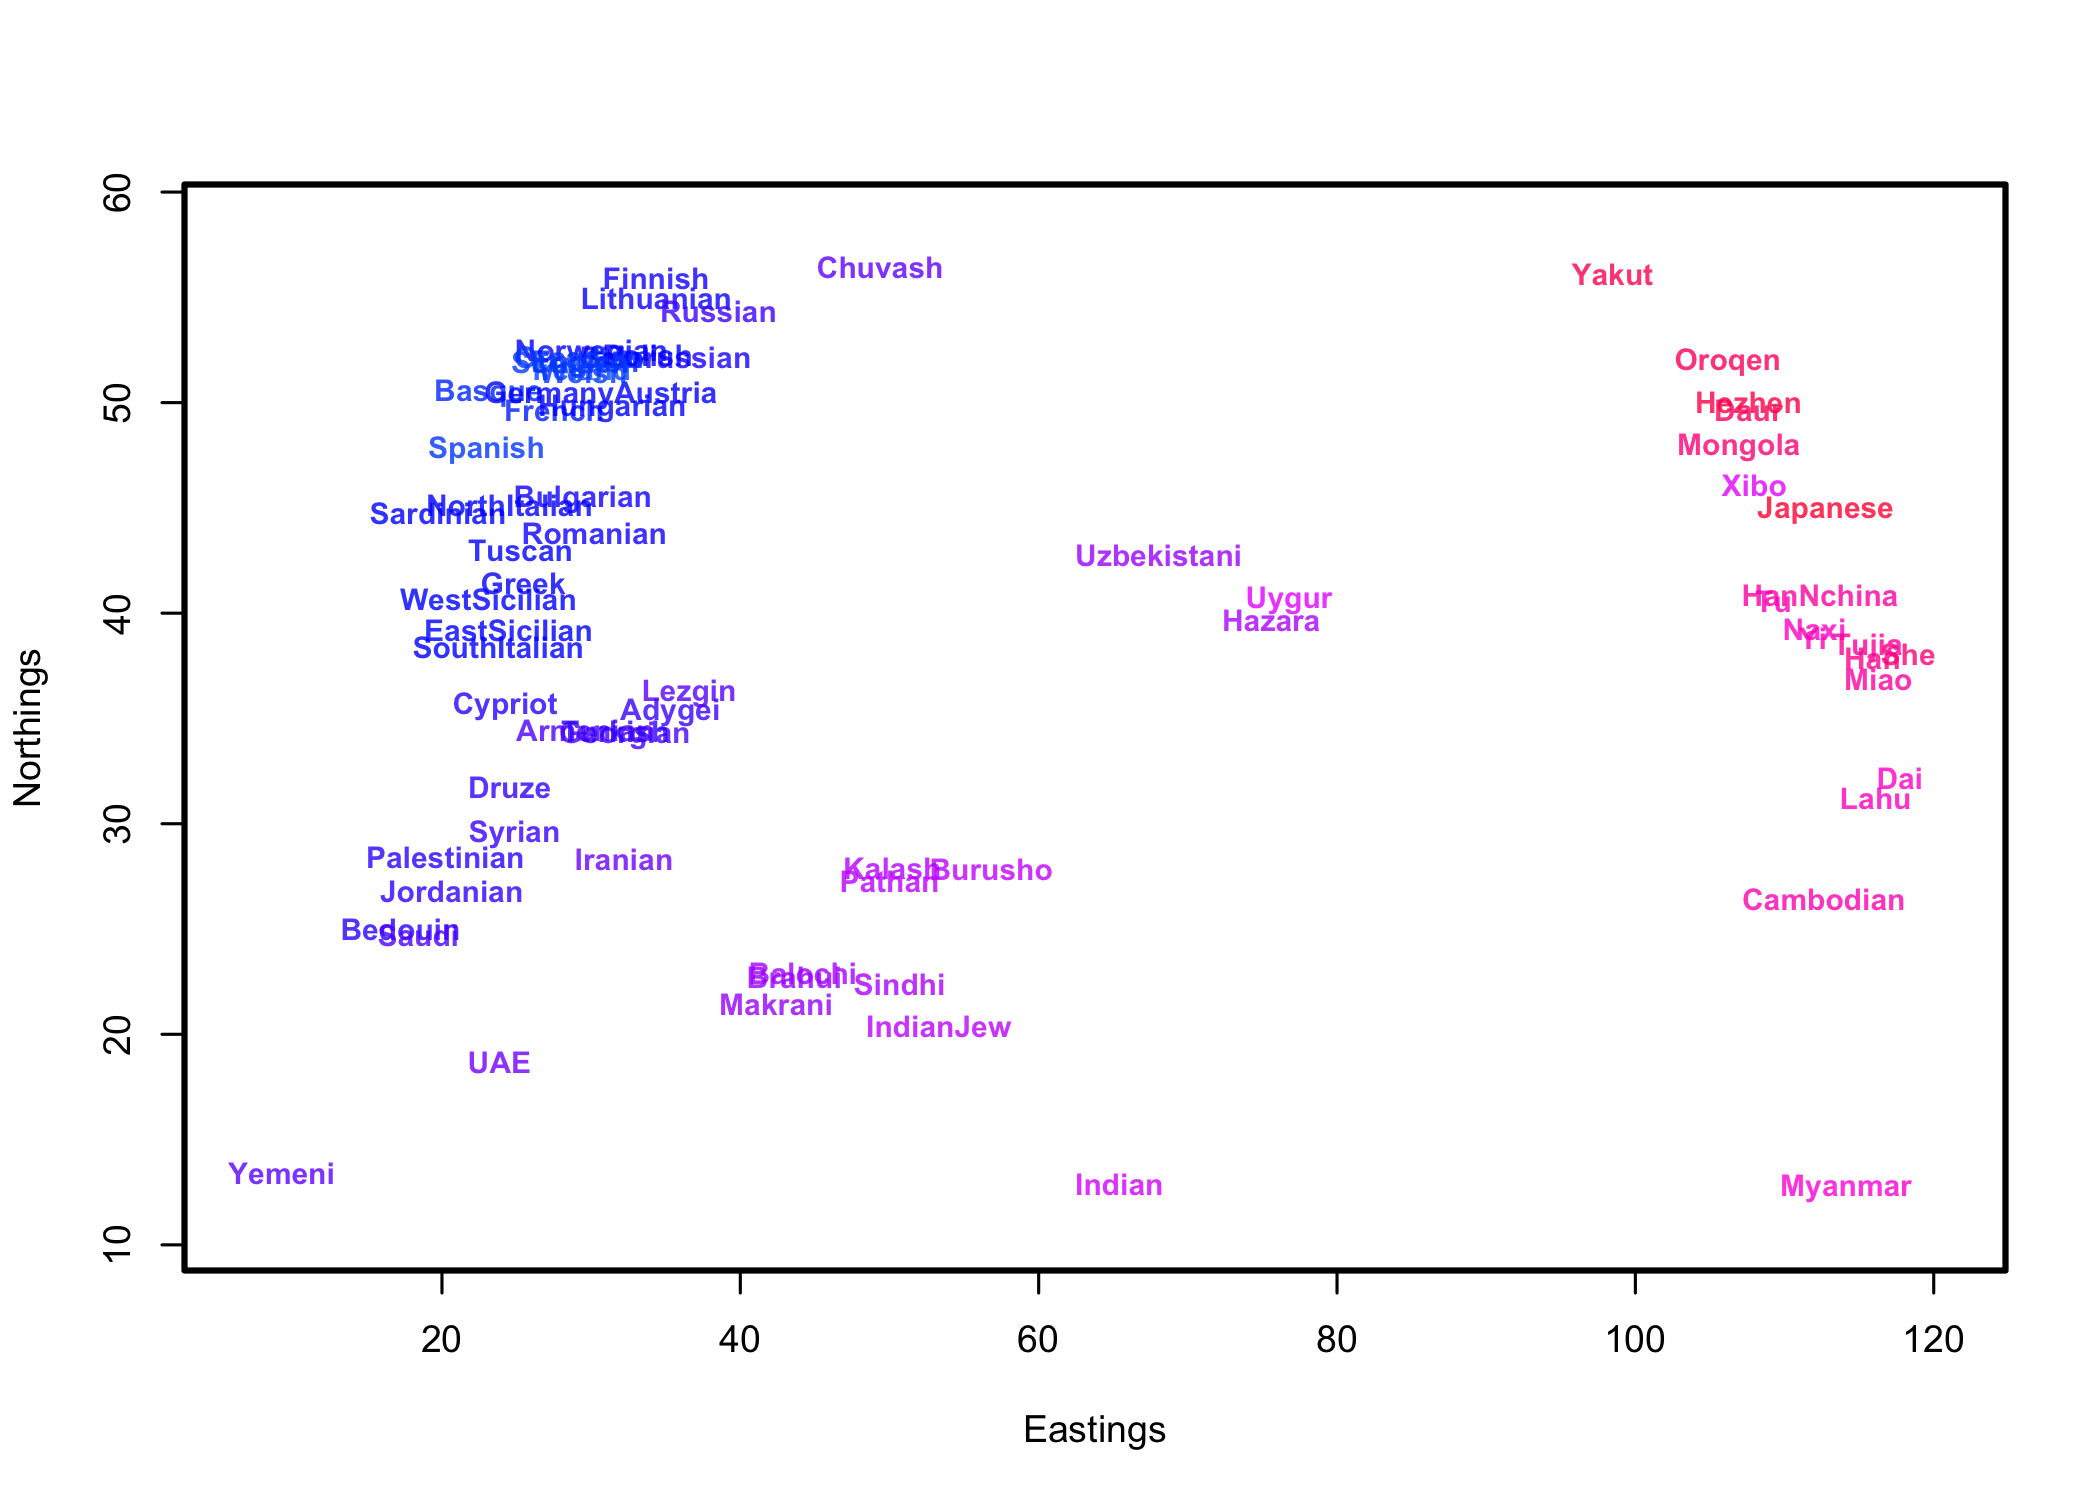
\includegraphics[width=2.8in,height=2.3in]{figs/globetrotter/globe_Eurasia_NoAd_map_indproc.png}}
	\caption{Map of human populations, inferred without admixture. (a) complete map; (b) close up of Eurasian 
populations.}\label{sfig:globe_noad_maps}
%(b) close up African populations; (c) close up of all non-African populations;
\end{figure}

We recover evidence for several major population expansions and colonization routes in human pre-history.  We can see evidence of these expansions by examining the relationship between observed and estimated pairwise distance between the daughter populations of a putative expansion event.   As can be seen in Figure \ref{sfig:expansion_scenarios}\subref{expansion_inference}, populations that have recently expanded on the landscape are less differentiated both from each other and from their parent population than would be expected from their geographic separation, and this fact is reflected in the decreased ratio between estimated and observed pairwise distances between members of an expansion event.

In the SpaceMix analysis of the human genetic data, the scale of inferred inter-population distance within Africa is much greater than that between any other group (see SuppMat Fig. \ref{sfig:globe_noad_distcomp}), and the slope of the relationship between observed and estimated distances between populations on each continent decays with distance from Africa.  This pattern is consistent with a history of human colonization events characterized by serial bottlenecks, including an out-of-Africa expansion, an expansion into East Asia, and twin expansions into the Americas and Oceania (REFS).  In addition, we see that both the populations in the Americas and those in Oceania cluster close to the East Asian populations, but that the two clusters are on opposite sides.  The proximity of these groups to the East Asians represents the fact that both groups share an ancestral population in the relatively recent past with East Asian populations(REF?), but that the expansion events induced independent drift trajectories in both waves of colonization.

We also see intriguing evidence for potential admixture in the placement of the Chuvash, Uzbekistani, Hazara, and Uygur populations, which choose locations intermediate between Europe and East Asia.  Notably, the Xibo who are sampled from a geographic location close to the Uygur, choose a geogenetic location within the East Asian samples.  The placement of the Moroccan, Mozabite, and Ethiopian populations, which choose locations between the western Eurasian cluster and the African cluster, is also suggestive of potential admixture.  To investigate possible patterns of admixture further, we ran a SpaceMix analysis in which we estimated the parameters of the spatial covariance matrix along with, for each population, a location, a source of admixture, and the magnitude of that admixture.

The biggest change between the geogenetic map of human populations inferred with admixture and that without is the positioning of African samples with respect to the rest of the world.  The relatively large geogenetic distances between these groups reflects the fact that Eurasian, North African, Oceanian, and American populations all share relatively large amounts of drift not shared with the Sub-Saharan African samples. The inclusion of admixture allows samples that fall intermediate between Sub-Saharan Africa and North Africa and the Middle East to move closer to one or the other, which, in turn, allows each of those major clusters to move relatively farther apart.  The Ethiopian and Ethiopian Jewish samples move to be closer to the Sub-Saharan samples than the rest of the North African samples, but draw substantial amounts of admixture ($\sim 40\%$) from close to where the Egyptian sample has positioned itself in the the Middle East cluster, as do the Sandawe. The SanKhomani draw admixture from near Syria, which may reflect multiple distinct geographic sources of admixture as discussed by \citep{Hellenthal} and \citep{Joe}. \gc{CHECK Joe's San paper}
Interestingly the Bantu South African sample, though it moves to join the other Bantu populations, draws admixture from close to the San populations. This is consistent with previous signals of the expansion of Bantu-speaking peoples into southern Africa (Pickrell et al 2012;Jakoboson, Hellenthal 2014). 

The majority North African populations (Egyptian, Tunisian, Morocan, Mozabite) move to join the Middle Eastern populations (positioning in rough accord with their sampling location along North Africa), and draw admixture from near the Ethiopian samples. All of the Middle Eastern samples draw admixture from close to the location chosen by the Ethiopian samples and where most of North African samples draw admixture from. It seems likely that this spread of populations represents North African influence. 


%%%%%%%%%
%Now instead of occupying an intermediate position the two Ethiopian samples draw a substantial proportion of their ancestry ($\sim 40\%$) from close to where the Egyptian sample has positioned itself in the the middle East cluster. The Sandawe population also draw a substantial portion of their ancestry from the middle east cluster.  Where's the Hadza going? Reciprocally, our North African samples (Egyptian, Tunisian, Morocan, Mozabite), having moved to join the middle eastern populations draw ancestry from close to the Ethiopian samples. 

%Hellenthal et al infer 2 admixture events and 3 admixture sources for the San Khomani: 1 event from the Bantu peoples in South Africa, and 1 event from a combination of northern European and southeast Asian populations.  

A number of other populations draw admixture from Africa. The Sindhi, Makrani, and Brahui draw admixture from close to the location of the Bantu samples, and the Balochi and Kalash draw admixture from some distance away from African populations.  Of the European samples, the Spanish and the East and West Sicilian samples all draw small amounts of admixture from close the Ethiopian samples presumably reflecting a North African ancestry component (Bustamante, and Reich). 

The other dominant signal of admixture is between East and West Eurasia. The majority of samples maintain their relative positions within each of these groups; however, several of the populations that chose locations intermediate between eastern and western Eurasia now move towards one side, and draw admixture from the other.  The Uzbekistani and Hazara samples move to be closer to the East Asian samples, while drawing a substantial admixture proportion from close to where the Georgian and Armenian samples have located themselves, while conversely the Uygur sample moves to be close to the Burusho, Kalash, and Pathan samples. The Tu sample (who locate to East Asia) draw a small amount of ancestry from close to where the Uygur have positioned themselves.
The Chuvash move close to Russian and Lithuanian samples, drawing admixture from close to the Yakut; the Turkish sample also draws a smaller amount of admixture from here. There are a number of other East-West connections: the Russian, Adygei samples have admixture from a location ``north'' of our East Asian samples, and Cambodia draws admixture from close to the Eygptian sample (as was also noted by Treemix, Globetrotter). 

There are a number of samples that draw admixture from locations that are not immediately interpretable.  For example, the Hadza and Bantu Kenyan samples draw admixture from somewhat close to India, and the Xibo and Yakut from close to ``northwest'' of Europe.  The Pathan draw admixture from a location far from any other samples' locations, but close to where India also draws admixture from. The Myanmar and the Burusho samples both draw admixture far from the locations estimated for other samples as well.% check Indian Jew

There are a number of possible explanations for these results. As we only allow a single admixture arrow for each sample, populations with multiple, geographically distinct, sources of admixture may be choosing admixture locations that average over the sources. This may be the case for the Hadza and Bantu Keynan samples.  A second possibility is that the relatively harsh prior on admixture proportion forces samples to choose lower proportions of admixture from locations that overshoot their true sources; this may explain the XIbo and Yakut admixture locations. A final explanation is that good proxies for the sources of admixture may not be included in our sampling, either because of of the limited geographic sampling of current day populations, or because of old admixture events from populations that are no long extant. The admixture into the Indians and Pathan may be an example of this, as has been hypothesized by Moorjani and Reich. %..... India Jew were are you? 

In the Supplementary Figures XXXX-ZZZZZ we show the results of other independent MCMC analyses on these data. The broad-scale patterns and results discussed above are consistent across these runs. However, as is to be expected, there is significant heterogeneity in the exact layout of sample and admixture locations. For example, there is some play, among MCMC runs, in the internal orientation of the African locations with respect to Eurasia.  Samples that draw a significant amount of admixture, such the central Asian populations (Uygur, Hazara and Uzibeckistani), switch their locations with that of their source of admixture (as was also seen across MCMC runs in the warbler data analysis). Similarly the Ethiopian and Ethiopian Jews choose locations, in some MCMC runs, close to the other North African samples, and draw admixture from near the Sub-Saharan samples (as do the other North African samples).

\begin{figure}
	\centering
		\subcaptionbox{Inferred map of human populations \label{globe_all_ad_map}}
			{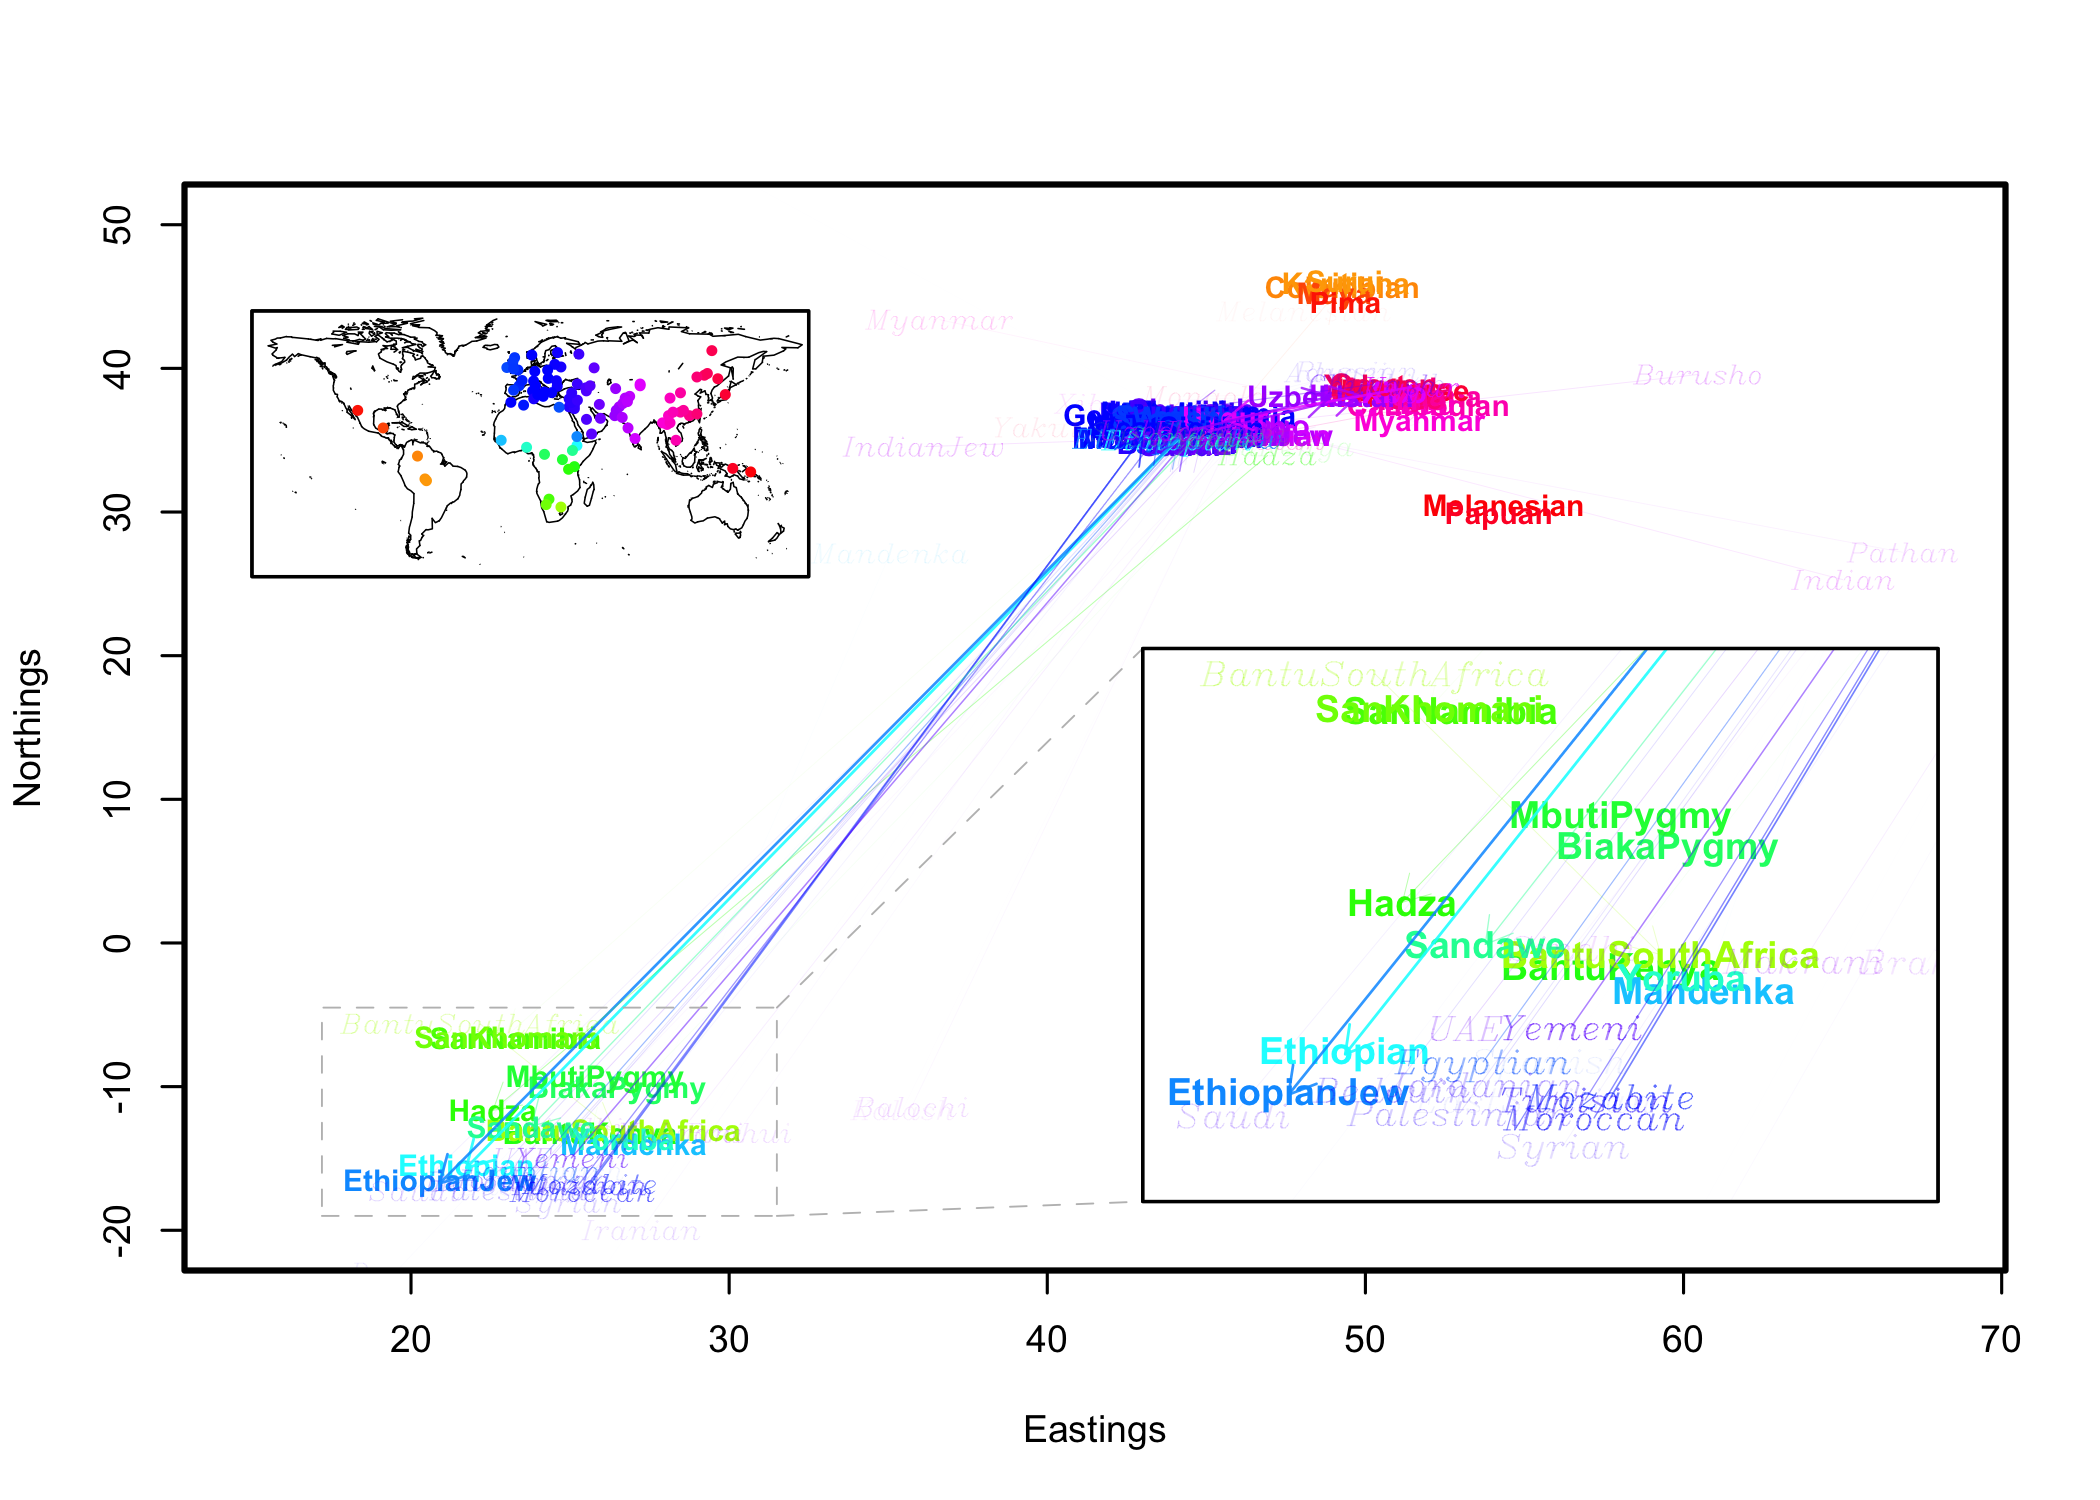
\includegraphics[width=2.8in,height=2.3in]{figs/globetrotter/globe_Ad_map_AfricaInset.png}}
		\subcaptionbox{Closeup of Eurasian populations \label{globe_eurasia_ad_map}}
			{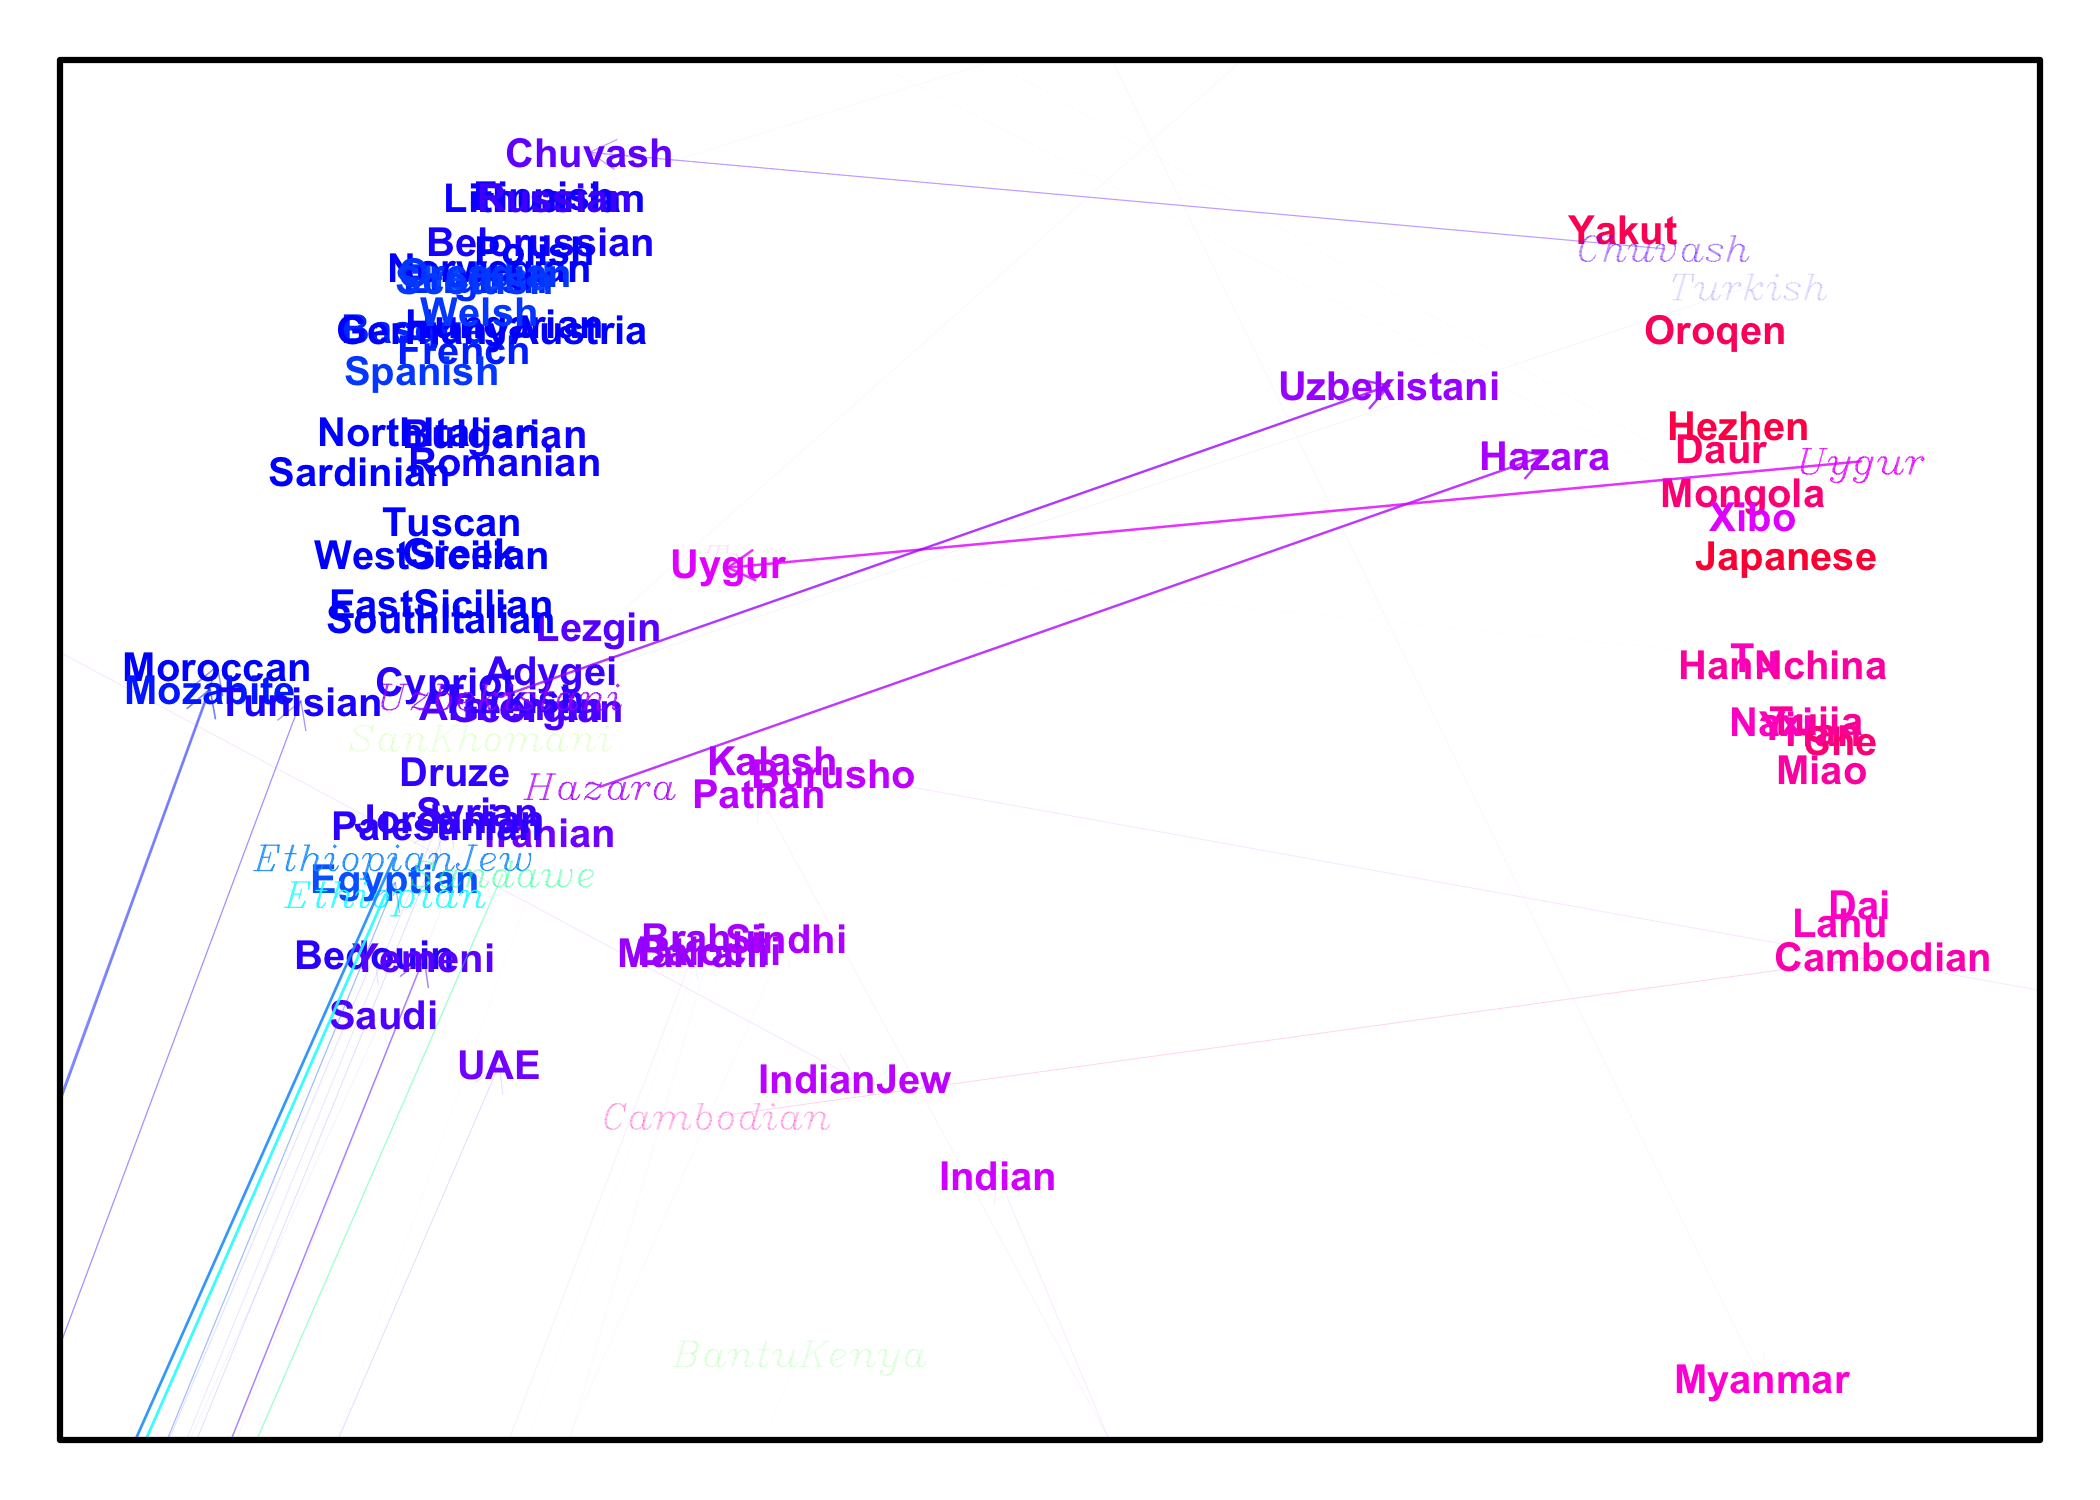
\includegraphics[width=2.8in,height=2.3in]{figs/globetrotter/eurasia_Ad_map_indproc.png}}
		\subcaptionbox{Inferred admixture proportions for human populations \label{globe_ad_props}}
			{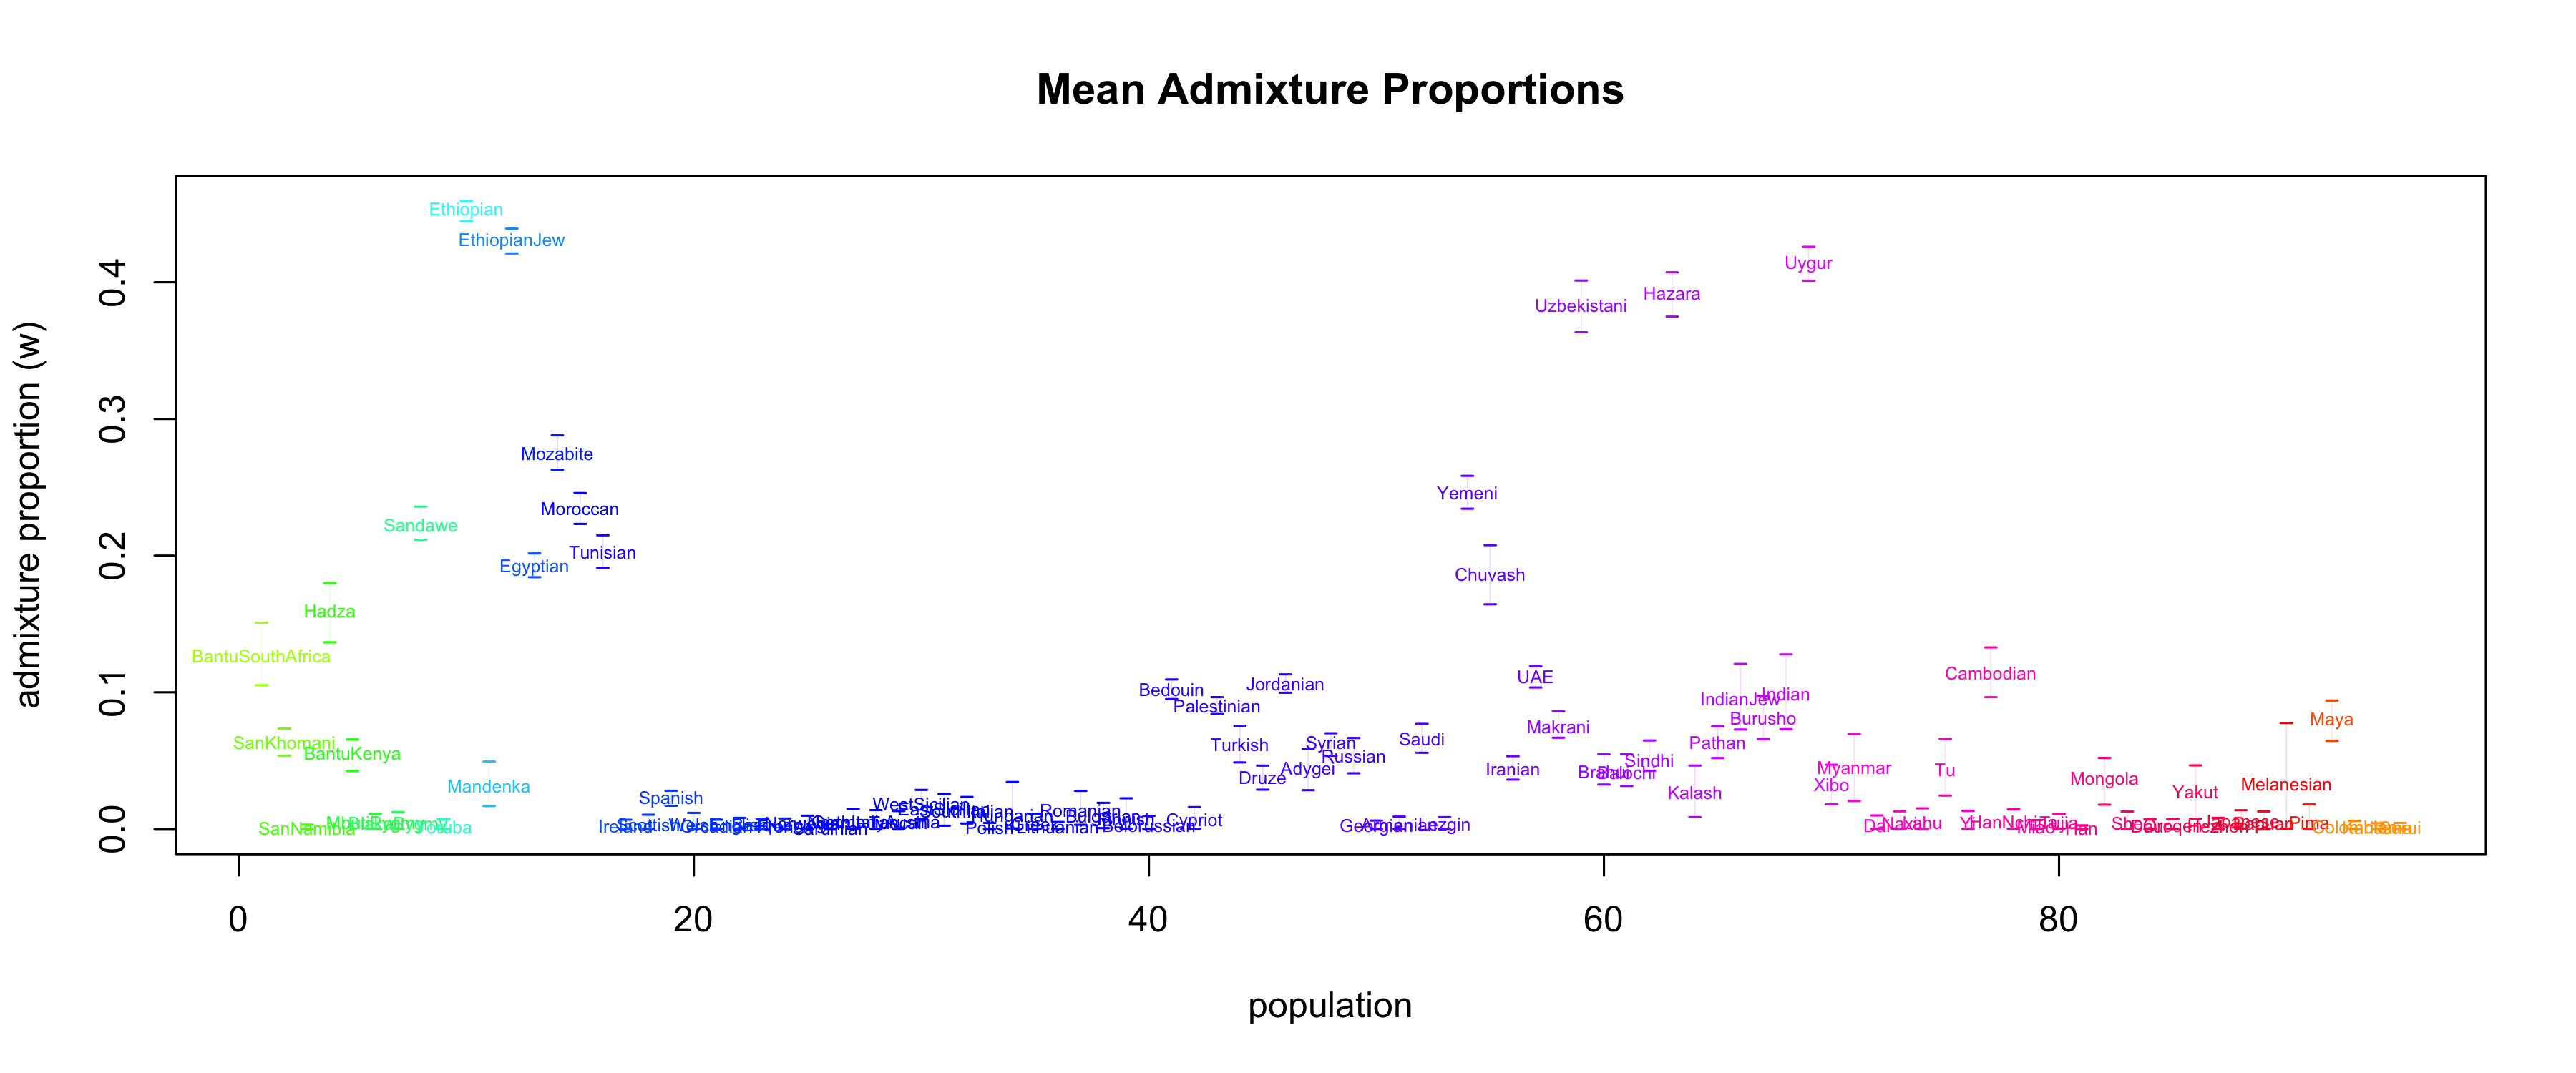
\includegraphics[width=5.6in,height=2.33in]{figs/globetrotter/globe_Ad_proportions.png}}
	\caption{Map of human populations, inferred with admixture. (a) complete map; (b) close up of Eurasian populations; c) mean admixture proportions for each population}\label{sfig:globe_ad_maps}
\end{figure}


\section*{Conclusion}
In this paper we have presented a statistical framework for modeling the geography of population structure from genomic sequencing data.
We have demonstrated that the method, SpaceMix, is able to accurately present patterns of population structure of a variety of simulated scenarios, which included the effects of spatially heterogeneous migration, population expansion, and population admixture.  In our empirical applications of SpaceMix, we have largely recovered previously estimated population relationships in a circum-Tibetan sample of greenish warblers and in a global sample of human populations, while also providing a novel way to depict these relationships.  The geogenetic maps SpaceMix generates serve as simple, intuitive, and powerful summaries of patterns of population structure.

Within the constellation of existing methods for inferring and illustrating patterns of population structure, SpaceMix falls between methods that use model-based inference to infer population trees, such as TreeMix, mixmapper, or Reich et al's \textit{f}-statistics, and methods that use dimensionality reduction to visualize patterns of structure on a map.  SpaceMix, unlike methods such as STRUCTURE or Geneland, does not infer hierarchical population structure, but it can be used as a useful guide in those analyses.

\subsection*{Caveats}
The patterns of genetic variation observed in modern populations are the product of a complex history of demographic processes.  We choose to model those patterns as the outcome of a process of spatially determined migration, and, although we have included statistical elements to accommodate deviations from spatial expectations (by, e.g., estimating population locations, allowing population-specific drift effects in the nugget parameters, and allowing the inference of admixture), it goes without saying that the true history of a sample of empirical populations is vastly more complex than any model we could create, and, as such, SpaceMix results should be interpreted with caution.

Three factors in particular stand out as potential sources of difficulty for the model.  The first is that there may be empirical datasets for which the assumption of IBD is inappropriate.  In taxa that migrate from their sampled locations and breed more or less panmictically elsewhere (or in the case of some broadcast spawners), a geogenetic map inferred by SpaceMix may bear no relation to the observed sample locations, and thus may be difficult to parse.  However, cases in which there is little or no concordance between the observed and inferred geography may also prove the most interesting and informative.

The second caveat is that, in the current release of SpaceMix, each population is allowed only a single source of admixture.  In many cases, modern day populations will be amalgams of many different historical groups, and the inability to model that history of multiple admixtures may produce results that are difficult to interpret (e.g., the inferred source of admixture falls in the middle of the locations of a population's true parental populations).  Although it is statistically and computationally possible to allow each population to choose more than one source of admixture, we were concerned about both the identifiability and the interpretability of such a model, but there may be empirical datasets in which such a modeling scheme is required to effectively map patterns of population structure.

Third, the landscape of allele frequencies on which the sources of admixture for the sampled populations are estimated is entirely informed by the placement of those modern samples.  However, it will almost certainly be the case that the true history of population admixture occurred at different points in space (and deeper in time), and between populations that are ancestral to those in the modern sample.  The increased sequencing of ancient DNA (skoglund, jakobsson, etc.) promises an interesting way forward on that front (and it will also be exciting to learn where ancient individuals fall on modern maps, as well as how the inclusion of ancient individuals changes the configuration of those maps).

\section*{Future Directions}

As noted in the third caveat above, the ancestral populations that have donated to the genetic makeup of modern day samples will not be among the samples in the current analysis, and therefore the inferred geography of admixture may only coarsely approximate the truth (depending on the complexity of the demographic history and the extent to which daughter populations of that ancestral admixture source both resemble their parents and have stayed put, geographically).  The inclusion of ancient DNA samples in the analyzed sample offers an intriguing way forward in getting better representation of the ancestral populations from which the ancestors of modern samples received their admixture.  However, it is also possible to model shared drift as a spatiotemporal Gaussian process, in which covariance in allele frequencies decays with distance both in space and in time.  In this model, which we are currently developing, ancient DNA samples can `calibrate' allele frequency landscapes at points in the past, and modern day samples may draw admixture from estimated coordinates in space-time.

\section*{Methods}
As described above, we have developed an algorithm, called SpaceMix, that uses the standardized sample allele frequency covariance and the the likelihood equation in equation \eqref{eq:admixed_post_prob} to simultaneously estimate the posterior distribution of the population locations, $G'$, their sources of admixture, $\identifyadmixsource{G}$, their admixture proportions, $w$, their independent drift parameters, $\eta$, and the parameters of the model of isolation by distance, $\vec{\alpha}$.  The inference procedure has two main components: (1) the derivation of the standardized sample allele frequency covariance matrix, and (2) a Markov chain Monte Carlo algorithm that samples parameter values from the posterior distribution.  Here, we describe these procedures in detail.

\subsection*{Deriving the standardized sample covariance}
% In the section on the normal approximation to drift, we describe how genetic drift - serial binomial sampling of allele frequencies through time - can be approximated as normally distributed change in allele frequencies around some ancestral mean, which we call $\epsilon_A$.  Under this normal approximation, the frequency of an allele in daughter population $B$ (sampled at some later point in time) can be described by the following equation,
% %
% \begin{equation}
% \label{eq:normal_drift}
% \epsilon_B \sim N(\epsilon_A,\delta_B(\epsilon_A)(1-\epsilon_A)),
% \end{equation}
% %
% where $\delta_B$ is the amount of drift separating $A$ and $B$.  This drift parameter is approximately equal to $\frac{t}{2N_e}$, where $t$ is time in generations separating $A$ and $B$, and $N_e$ is the constant effective population size.  Note that the binomial variance term in the normal variance in \eqref{eq:normal_drift} ignores the fact that the drift variance will change from generation to generation due to changes in the frequency of $\epsilon$ within a population over time.  Note also that this approximation works best for alleles at intermediate frequency, which are less likely to be lost or fixed during the interval separating the sampling of $A$ and $B$.  However, if the extent of drift is sufficiently limited (time scales are short or population sizes are large), the approximation of inter-generational binomial sampling to Brownian motion is good.  

% Among populations, the differentiating process of drift is counteracted by the homogenizing force of migration, so that populations with higher levels of historical or ongoing migration can be thought of as having more shared drift, i.e.\ stronger covariance in their allele frequency deviation around the ancestral (or global) mean.  Following Tobler's law (``everything is related to everything else, but near things are more related than distant things), we assume that the rate of migration between populations is inversely proportional to their geographic separation, such that the covariance in allele frequencies across loci between a pair of samples separated by a small distance is greater than that between a pair separated by a large distance.  

% We model the population frequencies at a locus as multivariate normal (MVN) with mean $\epsilon$ and covariance matrix $\epsilon(1 - \epsilon)\Omega$.  The multivariate normal distribution offers a natural statistical framework for describing this covariance, which may be straightforwardly modeled as a parametric function of any pairwise distance variable.

% We wish to model the covariance between populations as the result of a spatial process, in which migration rates between nearby populations are higher than between distant ones, so that a population has higher covariance with a close neighbor than with a more distant population.  We choose as the form of our parametric covariance matrix a simple and flexible model, with an exponential decay of allele frequency covariance with geographic distance (Wasser et al 2004, Bradburd, Ralph, and Coop 2013).  The covariance between population allele frequencies in populations $i$ and $j$ is 
% %
% \begin{equation}
% %\label{eq:spatial_covariance}
% \Omega_{i,j} = \frac{1}{\alpha_0} \text{exp} \left(	\left( \alpha_1D_{i,j} \right)^{\alpha_2} \right) \text{,}
% \end{equation}
% %
% where $D_{i,j}$ is the geographic distance between population $i$ and $j$ (and therefore a function of their locations, $G_i$ and $G_j$), $\alpha_0$ controls the within-population variance, or the covariance when distance between points is 0 (the sill of the covariance matrix),  $\alpha_1$ controls the rate of the decay of covariance per unit pairwise distance, and $\alpha_2$ determines the shape of that decay. While previously we and others have used a logit link function combined with binomial sampling to model the sample frequencies \citep{Wasser, Bradburd}, here we chose to treat these standardized frequencies $\hat{f}_{\ell}$, as multivariate normal across populations \citep[]{Treemix}. To accommodate the effect of finite sample size we introduce ``nuggets'' of population-specific variance terms, on the diagonal of allelic covariance matrix,which accommodate the effects of both sampling and unshared genetic drift.
% %
% \begin{equation}
% %\label{eq:spatial_covariance2}
% \Omega_{i,j} = \frac{1}{\alpha_0} \text{exp} \left(	\left( \alpha_1D_{i,j} \right)^{\alpha_2} \right) + \delta(\bar{S}^{-1} + \eta) \text{,}
% \end{equation}
% %
% where $\delta_{i,j}$ is the indicator function $1$ if $i=j$, and $0$ otherwise. Our $\eta$ is a vector of population-specific variances, where $\eta_k$, the nugget estimated in population $k$, represents any genetic drift (or more generally excess allele frequency variance) not captured by our spatial model. Finally $\bar{S}$ is a vector of the mean sample sizes in each population, where $\bar{S}_k$, is the mean sample size across all loci in population $k$.  


We then assume that our sample allele frequencies at a locus across populations are given by
%
\begin{equation}
\hat{f}_{\ell} \sim MVN(\epsilon_{\ell}, \epsilon_{\ell} (1-\epsilon_{\ell})\Omega)
\end{equation}
%
with $\Omega$ given by equation \eqref{eq:spatial_covariance2},  where the $\epsilon_{\ell}(1 - \epsilon_{\ell})  \bar{S}^{-1}$ on the diagonal of the covariance matrix captures, to first approximation, the effects of sampling.

%Given the assumption of multivariate normality for our sample frequencies, it follows that the sample covariance of our standardized sample frequencies calculated across loci ($\widehat{\Omega} = f f^T$)  is Wishart distributed with degrees of freedom equal to the number of loci ($L$) across which the covariance is calculated.
%That is, 
%
%\begin{equation}
%\label{eq:wishart_dist}
%L \widehat{\Omega} \sim \mathcal{W}\left( \Omega, L	\right)
%\end{equation}
%
If we knew $\epsilon$ we can calculate an estimate of the covariance matrix ($\Omega$) across loci as 
%
\begin{equation}
%\label{eq:sample_cov}
\widehat{\Omega} = \frac{1}{L} \sum_{\ell=1}^{L} \frac{(\hat{f}_{\ell_{\ell}}  - \epsilon_{\ell}) (\hat{f}_{\ell}  - \epsilon_{\ell})^T}{\epsilon_{\ell}(1-\epsilon_{\ell})} \text{.}
\end{equation}
%
Then, if we define our standardized sample allele frequencies, $X_\ell$, as
%
\begin{equation}
%\label{eq:standardized_sample_freqs}
X_\ell = (\hat{f}_{\ell}  - \epsilon_{\ell})/\sqrt{\epsilon_{\ell}(1-\epsilon_{\ell})}\text{,}
\end{equation}
%
the expression given in equation \eqref{eq:sample_cov} gives the sample covariance matrix of our standardized sample allele frequencies. Then $L\widehat{\Omega} = X X^T$  is Wishart distributed with degrees of freedom equal to the number of loci ($L$) across which the covariance is calculated. 

%\mathcal{W}\left(L \widehat{\Omega} \mid  \Omega,L \right)
%Given the assumption of multivariate normality for our sample frequencies, it follows that this sample covariance of our standardized sample frequencies calculated across loci ($\widehat{\Omega} = X X^T$)  is Wishart distributed with degrees of freedom equal to the number of loci ($L$) across which the covariance is calculated.
%That is, 
%
%\begin{equation}
%\label{eq:wishart_dist}
%P(\widehat{\Omega} \mid \Omega) =
%\end{equation}
%
However, we do not have the `ancestral' frequency $\epsilon$. Instead we mean-center and normalize our observations at a locus using the weighted mean sample frequency in place of $\epsilon$.  Recall that the sample allele frequency at locus $\ell$ in population $k$ is given by $\hat{f}_{\ell,k} = C_{\ell,k}/S_{\ell,k}$.  We wish to calculate a sample mean frequency at each locus weighted by the sample size in each population.  As sample size may vary across loci, we first calculate $\bar{S}_k$, the mean sample size in population $k$, as $\bar{S}_k = \frac{1}{L}\sum_{\ell=1}^L S_{\ell,k}$.  We then calculate the weighted sample mean frequency at locus $\ell$ 
%
\begin{equation}
%\label{eq:sample_mean_freq}
\bar{f}_{\ell} = \frac{1}{\sum_K S_{\ell,k}} \sum_K \hat{f}_{\ell,k} S_{\ell,k}
\end{equation}
%We approximate the binomial variance at each locus by $\bar{f}_{\ell}(1-\bar{f}_{\ell})$.  To avoid modeling the heterogeneous effect of this variance across loci, we standardize by this variance. 
We call the mean standardized allele frequency in population $k$ $X_{\ell,k}^{\prime}$, and calculate them as follows:
%  \gc{Graham changed this to }
\begin{equation}
%\label{eq:MCN_freqs}
\hat{X_{\ell,k}} = \frac{ \hat{f}_{\ell,k} - \bar{f}_{\ell} } {\sqrt{\bar{f}_{\ell}(1-\bar{f}_{\ell})}}
\end{equation}
%
This is equivalent to taking our normalized vector of sample frequencies
\begin{equation}
Y_{\ell} = \frac{ \hat{f}_{\ell,k} } {\sqrt{\bar{f}_{\ell}(1-\bar{f}_{\ell})}}
\end{equation}
and writing $X_{\ell}^{\prime} = T Y_{\ell} $ where $T$ is the mean centering matrix, whose elements are given by 
\begin{equation}
T_{ij} = \delta_{ij}  -  \frac{\bar{S}_j}{\sum\limits_{k=1}^{K} \bar{S}_j	} 
\end{equation}
Therefore, we assume that
\begin{equation}
\hat{X_{\ell}} \sim MVN(0, T^T \Omega T)
\end{equation}
the mean centering acts to to reduce the covariance among populations in $\hat{X_{\ell}}$ compared to $X_{\ell}$, and can induce negative covariance between distant populations (as they are often on either side of the mean). In addition the covariance matrix of our mean centered frequencies has rank $K-1$ rather than $K$, as any one of our mean centered frequencies could be written as a linear function of the others. 

This means that $T^T \Omega T$ is not invertible, and so can not be used directly in our Wishart likelihood. To circumvent this problem we take the $QR$ decomposition of the matrix $T$, and form a projection matrix $\Psi= Q_{,-K}$ dropping the $K^{th}$ column of $Q$. We then write our Wishart likelihood as
\begin{equation} \label{eq:projected_wishart_dist}
P(\widehat{\Omega} \mid \Omega) = \mathcal{W}\left( \Psi^T YY^T \Psi \mid  \Psi^{T}   \Omega   \Psi,L \right) \text{.}
\end{equation}
this procedure avoids the reduced rank of our covariance matrices. 

% \gc{BLAH}
% Note, by using the sample mean frequency to mean-center our observations, we lose a degree of freedom, and reduce the covariance across loci between populations (sometimes inducing negative covariance between distant populations). We accommodate the extra sampling noise distortion and the reduced rank of the covariance matrix by assuming that our
% %
% \begin{equation}
% X_{\ell} \sim MVN(0, \Omega^{\prime} )
% \end{equation}
% %
% where $\Omega^{\prime}$ is a simple transform of $\Omega$.  Specifically, 
% %
% \begin{equation}
% \Omega^{\prime} = \Psi^{T}   \Omega   \Psi \text{,}
% \label{eq:projected_covariance}
% \end{equation}
% %
% where
%  %
% $\Psi$ is a projection matrix that is used to project our degenerate covariance matrix back into full rank.  This projection matrix is given by
% \begin{equation}
% \Psi = \text{qr.Q}(\text{qr}(\Upsilon))[,1:(k-1)] \text{,}
% \end{equation}
% %
% where $\text{qr}$ is the QR decomposition, $\text{qr.Q}$ returns the original matrix on which the QR decomposition was performed, and
%  $\Upsilon$, a matrix to mean-center the sample allele frequencies, weighting by the mean sample size in each population, is given by 
% \begin{equation}
% T_{ij} = \delta_{ij}  -  \frac{\bar{S}_j}{\sum\limits_{i=1}^{K} \bar{S}_j	} 
% \end{equation}
% %
% \[ \Upsilon = \left( 
% \begin{array}{cccc}
% 1 - \frac{\bar{S}_1}{\sum\limits_{i=1}^{K} \bar{S}_k	} & -\frac{\bar{S}_2}{\sum\limits_{i=1}^{K} \bar{S}_k	} & \ldots & -\frac{\bar{S}_k}{\sum\limits_{i=1}^{K} \bar{S}_k	} \\
% -\frac{\bar{S}_1}{\sum\limits_{i=1}^{K} \bar{S}_k	} & 1 - \frac{\bar{S}_2}{\sum\limits_{i=1}^{K} \bar{S}_k	} & \ldots & -\frac{\bar{S}_k}{\sum\limits_{i=1}^{K} \bar{S}_k	} \\
% \vdots & \vdots & \ddots  & \vdots	\\
% -\frac{\bar{S}_1}{\sum\limits_{i=1}^{K} \bar{S}_k	} & -\frac{\bar{S}_2}{\sum\limits_{i=1}^{K} \bar{S}_k	} & \ldots  & 1 - \frac{\bar{S}_k}{\sum\limits_{i=1}^{K} \bar{S}_k	} 
% \end{array} \right).\]\\
% %



%  $\Upsilon$, a matrix to mean-center the sample allele frequencies, weighting by the mean sample size in each population, is given by 
% %
% \[ \Upsilon = \left( 
% \begin{array}{cccc}
% 1 - \frac{\bar{S}_1}{\sum\limits_{i=1}^{K} \bar{S}_k	} & -\frac{\bar{S}_2}{\sum\limits_{i=1}^{K} \bar{S}_k	} & \ldots & -\frac{\bar{S}_k}{\sum\limits_{i=1}^{K} \bar{S}_k	} \\
% -\frac{\bar{S}_1}{\sum\limits_{i=1}^{K} \bar{S}_k	} & 1 - \frac{\bar{S}_2}{\sum\limits_{i=1}^{K} \bar{S}_k	} & \ldots & -\frac{\bar{S}_k}{\sum\limits_{i=1}^{K} \bar{S}_k	} \\
% \vdots & \vdots & \ddots  & \vdots	\\
% -\frac{\bar{S}_1}{\sum\limits_{i=1}^{K} \bar{S}_k	} & -\frac{\bar{S}_2}{\sum\limits_{i=1}^{K} \bar{S}_k	} & \ldots  & 1 - \frac{\bar{S}_k}{\sum\limits_{i=1}^{K} \bar{S}_k	} 
% \end{array} \right).\]\\
% %
% The standardized sample allele frequency covariance $\Omega^{\prime}$ is then simply given by $XX^{T}$, and the Wishart likelihood of the standardized sample covariance is taken as a function of the projected parametric covariance matrix as follows:
% %
% \begin{equation}
% \label{eq:projected_wishart_dist}
% P(\widehat{\Omega} \mid \Omega) = \mathcal{W}\left(L \widehat{\Omega^{\prime}} \mid  \Psi^{T}   \Omega   \Psi,L \right) \text{.}
% \end{equation}
%

%%%%%%%%%%%%%%%%%%%%%%%%%%%%%%%%
\subsection*{Markov chain Monte Carlo Inference Procedure}
The inference algorithm described here may be used to estimate the parameters of any of four possible models: (1) population locations are stationary, and they do not draw any admixture; (2) populations may choose their own locations, but not admixture; (3) populations may draw admixture, but are themselves stationary; (4) populations may both choose their own locations and draw admixture.  The free parameters in each of these models are given in Table \ref{tab:model_options}.

\begin{centering}
\begin{table}
\begin{tabular}{| >{\centering\arraybackslash}m{6cm} | >{\centering\arraybackslash}m{3cm} | l |}
	\hline
	\textbf{Model} & \textbf{No. Free Parameters} & \textbf{Parameters}\\ \hline
	stationary population locations, no admixture & $K + 3$	& $\alpha_0,\alpha_1,\alpha_2,\eta$	\\ \hline
	inferred population locations, \hspace{0.5cm}no admixture & $2K + 3$	& $\alpha_0,\alpha_1,\alpha_2,\eta,G^{\prime}$	\\ \hline
	stationary population locations, inferred admixture & $2K + 3$	& $\alpha_0,\alpha_1,\alpha_2,\eta,\identifyadmixsource{G},w$	\\ \hline
	inferred population locations, inferred admixture & $3K + 3$	&$\alpha_0,\alpha_1,\alpha_2,\eta,G^{\prime},\identifyadmixsource{G},w$	\\
	\hline
\end{tabular}
\caption{List of models that may be specified using SpaceMix, along with the number and identity of free parameters in each.}\label{tab:model_options}
\end{table}
\end{centering}

Below, we outline the inference procedure for the most parameter-rich model (inference on both population locations, their sources of admixture, and the proportions in which they draw admixture, in addition to inference of the parameters of the spatial covariance function).

We use a Bayesian MCMC approach to parameter inference, and specify priors on all parameters.  A table of all parameters, their descriptions, and their priors is given in Table \ref{tab:param_prior_tab}.

\begin{centering}
\begin{table}
\begin{tabular}{| >{\centering\arraybackslash}m{2.1cm} | m{6cm} | >{\centering\arraybackslash}m{6cm} |}
	\hline
	\textbf{Parameter} & \centering{\textbf{Description}} & \textbf{Prior}\\ \hline
	$\boldsymbol{\alpha_0}$ & 
		controls the sill of the covariance matrix & 
		$\alpha_0 \sim Exp(\lambda = 1/100)$\\ \hline
	$\boldsymbol{\alpha_1}$ & 
		controls the rate of the decay of covariance with distance & 
		$\alpha_1 \sim Exp(\lambda = 1)$\\ \hline
	$\boldsymbol{\alpha_2}$ & 
		controls the shape of the decay of covariance with distance & 
		$\alpha_2 \sim U(0.1,2)$\\ \hline
	$\boldsymbol{\eta_k}$ & 
		the nugget in population $k$ (population specific drift parameter)  & 
		$\eta_k \sim Exp(\lambda = 1)$\\ \hline
	$\boldsymbol{G_k^{\prime}}$ & 
		the estimated location of population $k$ &
		 $G_k^{\prime} \sim \mathcal{N}(\mu = G_k,\sigma = \frac{1}{2}\bar{D}(G))$ \\ \hline
	$\boldsymbol{w_k}$ &
		the proportion of admixture in population $k$ &
		$2 w_k \sim \beta(\alpha = 1,\beta = 100)$  \\ \hline
	$\boldsymbol{\identifyadmixsource{G_k}}$ &
		the estimated location of the source of admixture in population $k$ &
		$\identifyadmixsource{G_k} \sim \mathcal{N}(\mu = \bar{G},\sigma = 2 \bar{D}(G))$ \\
	\hline
\end{tabular}
\caption{List of parameters used in the SpaceMix models, along with their descriptions and priors.}\label{tab:param_prior_tab}
\end{table}
\end{centering}

Our inference algorithm proceeds is described in excruciating detail below.

We assume that the user has specified the following data: 
\begin{itemize}
\item the allelic count data, $C$, from $K$ population over $L$ variant loci, where $C_{\ell,k}$ gives the number of observations of a given allele at locus $\ell$ in population $k$. 
\item the sample size data, $S$, from $K$ population over $L$ variant loci, where $S_{\ell,k}$ gives the number of haplotypes sampled at locus $\ell$ in population $k$.
\item the geographic sampling locations, $G$, from each of the $K$ populations, where $G_k$ gives the longitude and latitude of the sampled individual(s).
\end{itemize}

Geographic location data may be missing, or generated randomly, for some or all of the samples; if so, the spatial priors on estimated population locations, $G^{\prime}$ and their sources of admixture, $\identifyadmixsource{G}$ will not be tethered to the true map. 

% standardized (mean-centered and normalized by variance) allele frequency, $X$, at each locus, and, from $X$, the 
\paragraph{Initiating the MCMC}
We then calculate the standardized sample covariance matrix $\widehat{\Omega}^{\prime}$ as outlined in the section ``Deriving the standardized sample covariance" above.  We calculate $\bar{S_k}$, the mean sample size across loci for population $k$, for each population as part of the standardization of the sample allele frequencies, and for use as $\bar{S_k}^{-1}$ as part of the spatial covariance function detailed in \eqref{eq:spatial_covariance2}.

Armed with the standardized sample covariance, the geographic sampling locations, and the inverse mean sample sizes across samples ($\widehat{\Omega}^{\prime}$, $G$, $\bar{S_k}^{-1}$), we may embark upon our analysis.

To initiate our MCMC, we specify starting values for each parameter.  We draw initial values for $\alpha_0$, $\alpha_1$, $\alpha_2$, $\eta$, and $w$ randomly from their priors.  We initiate $G^{\prime}$ at user-specified geographic sampling locations and $\identifyadmixsource{G}$ at randomly drawn, uniformly distributed values of latitude and longitude in the observed range of both axes.  

\paragraph{Overview of MCMC procedure}
%and the observed $\bar{S_k}^{-1}$, can be used to specif
%This parametric covariance matrix is then projected following equation \eqref{eq:projected_covariance}, using the projection matrix $\Psi$ described in the standardization of allele frequencies above. 
We use a Metropolis-Hastings update algorithm. In each iteration of the MCMC, one of our current set of parameter $\Theta= \{\alpha_0$, $\alpha_1$, $\alpha_2$, $\eta$, $w$, $G^{\prime}$, $\identifyadmixsource{G}\}$ is randomly chosen to be updated by proposing a new value.  In the cases of \{$\eta$, $w$, $G^{\prime}$, $\identifyadmixsource{G}$\}, where each population has its own parameters, a single population, $k$ is randomly selected and only its parameter value (e.g.\ $\eta_k$) is chosen to be updated. Below we outline the proposal distributions for each parameter. This gives us a proposed update to our set of parameters $\Theta^{NEW}$, which differs from $\Theta$ at only one entry.

The set of locations of populations and their sources of admixture specify a pairwise geographic distance matrix $D$, which, given the current $\vec{\alpha}$ and $\eta$ parameters, gives the admixed covariance matrix described in \eqref{eq:admixed_covariance_1}, $\identifyadmixsource{\Omega}$.  We then calculate the likelihood of the standardized sample covariance $\widehat{\Omega}^{\prime}$ following equation \eqref{eq:projected_wishart_dist} for the current set of parameters $P(\widehat{\Omega}^{\prime} \mid \identifyadmixsource{\Omega}(\Theta))$ and our proposed update to our set of parameters $P(\widehat{\Omega}^{\prime} \mid \identifyadmixsource{\Omega}(\Theta^{NEW}))$. We then calculate the prior probabilities of both sets of parameter values, $P(\Theta^{NEW}),~P(\Theta) $, following the priors given in Table \ref{tab:param_prior_tab}.


%We can then take the likelihood of the standardized sample covariance $\widehat{\Omega}^{\prime}$ following equation \eqref{eq:projected_wishart_dist}, $P(\widehat{\Omega} \mid \identifyadmixsource{\Omega}())$. 


We combine these together to give the Metropolis-Hastings ratio, \emph{R}, the probability of accepting the proposed parameter values $\Theta^{NEW}$:
\begin{equation}
R = \text{min}\left(1, \frac{(\widehat{\Omega}^{\prime} \mid \identifyadmixsource{\Omega}(\Theta^{NEW}))} {P(\widehat{\Omega}^{\prime} \mid \identifyadmixsource{\Omega}(\Theta))} 
				\frac{P(\Theta^{NEW})}{P(\Theta)} 	\right) \text{,}
			%	\frac{P(\theta^{\prime} \to \theta)}{P(\theta \to \theta^{\prime})}	
\label{eq:MH_algorithm}
\end{equation}
Note that all of our moves, described below, are symmetric so a Hastings ratio cancels through. If we accept our proposed move $\Theta$ is replaced by $\Theta^{NEW}$ and this is recorded, otherwise $\Theta^{NEW}$ is disgarded and we remain at $\Theta$. 

%\begin{equation}
%R = \text{min}\left(1, \frac{P(D \mid \theta^{\prime})} {P(D \mid \theta)} 
%				\frac{P(\theta^{\prime})}{P(\theta)} 
%				\frac{P(\theta^{\prime} \to \theta)}{P(\theta \to \theta^{\prime})}		\right) \text{,}
%\label{eq:MH_algorithm}
%\end{equation}

%where $\frac{P(D \mid \theta^{\prime})} {P(D \mid \theta)}$ gives the ratio of the likelihood of the data under the proposed parameter value to that under the current parameter value, $\frac{P(\theta^{\prime})}{P(\theta)}$ gives the ratio of the prior probability of the proposed parameter value to that of the current parameter value, and $\frac{P(\theta^{\prime} \to \theta)}{P(\theta \to \theta^{\prime})}$ is the Hastings ratio, or the ratio of the conditional probability of proposing the current parameter value given the proposed parameter value to that of proposing the proposed parameter value given the current parameter value (Hastings 1970, Gilks 1996).


\paragraph{Udates for $\vec{\alpha}$, $\eta$, and $w$.}
We propose updates to the values of the $\vec{\alpha}$, $\eta$, and $w$ parameters via a symmetric normal density with mean zero and its own variance given by the scale of the tuning parameter for that parameter.  For example $\alpha_0^{\prime} \sim \alpha_0 + \delta$, where $delta \sim \mathcal{N}(0,\sigma_{\alpha_0})$ and $\sigma_{\alpha_0}$ is scale of the tuning parameter.  For $\eta$ and $w$, each of which consists of $K$ parameters, each parameter receives its own idependent scale of the tuning parameter. If the proposed move takes the parameter outside the range of its prior, the move is rejected and we do not move in that iteration of the MCMC.

%\neq \sigma_{\alpha_1} \neq \sigma_{\alpha_2}$

%(e.g.\ - $\sigma_{\eta_{i}} \neq \sigma_{\eta_{j}}$)

\paragraph{Updates for geographic co-ordinates $G^{\prime}$ and $\identifyadmixsource{G}$}. Updates to the location parameters, $G^{\prime}$ and $\identifyadmixsource{G}$, are somewhat more complicated due to the curvature of the Earth (Eratosthenes, \textit{personal observation}).  Implementing updates via a symmetric normal density on estimated latitude and longitude directly, which would have the drawback of a) being naive to the continuity of the spherical manifold and b) vary the actual distance of the proposed move as a function of the current lat/long parameter values (e.g., a $1^{\circ}$ change in longitude at the equator is a larger distance than at the North Pole).  

Instead, we propose for a bearing and a distance traveled, and, given these two quantities and a starting position, calculate the latitude and longitude of the proposed location.  For example, in an update to the location of population $i$, $G^{\prime}_i$, we propose a distance traveled $\Delta_{{G^{\prime}}_i}$, where, e.g., $\Delta_{{G^{\prime}}_i}  \sim | \mathcal{N}(0,\sigma_{{G^{\prime}}_i})|$, and a bearing, $\gamma$, where $\gamma \sim U(0,2\pi)$.  Then we use the following equations to calculate the latitude and longitude of the proposed location:
\begin{align}
\text{proposed latitude} = \arcsin(\sin(\text{current latitude}) \: &\times\\  \notag
					\cos(\Delta) \times \cos(\text{current latitude}) \:&\times\\  \notag
					\sin(\Delta) \times \cos(\gamma))   \:&\phantom{\times}\\  \notag
\end{align}
and
\begin{align}
\text{proposed longitude} = & - \pi + (\text{current longitude} \; - \\ \notag
					 	&\hspace{1cm} \arctan(
							\sin(\gamma) \times
							\sin(\Delta) \times
							\cos(\text{current latitude}) , \\ \notag
						& \hspace{2cm} \cos(\Delta) - 
							\sin(\text{current latitude}) \times \\ \notag
						& \hspace{2cm} \sin(\text{proposed latitude})) + \pi) \; \bmod (2\pi) \\ \notag
\end{align}

where latitude and longitude are given in radians.  As with $\eta$ and $w$, the scales of the tuning parameters for the different populations and different location parameters ($G^{\prime}$ and $\identifyadmixsource{G}$) are independent.


\paragraph{Adaptive Metropolis-within-Gibbs proposal mechanism }.
We use an adaptive Metropolis-within-Gibbs proposal mechanism on each parameter (Roberts and Rosenthal 2008, Rosenthal 2010).  This mechanism attempts to maintain an acceptance proportion for each parameter as close as possible to 0.44 (optimal for one-dimensional proposal mechanisms; Roberts et al 1997, Roberts and Rosenthal 2001).  We implement this mechanism by creating, for each variable $i$, an associated variable $\zeta_i$, which gives the log of the standard deviation of the normal distribution from which parameter value updates are proposed.  As outlined above, in the cases of \{$\eta$, $w$, $G^{\prime}$, $\identifyadmixsource{G}$\}, for which each population receives a free parameter, each population gets its own value of $\zeta$.  

When we start our MCMC, $\zeta_i$ for all parameters is initiated at a value of 0, which gives a proposal distribution variance of 1.  We then proceed to track the acceptance rate, $r_i$ for each parameter in windows of 50 MCMC iterations, and, after the $n$th set of 50 iterations, we adjust $\zeta_i$ by an "adaption amount," which is added to $\zeta_i$ if the acceptance proportion in the $n$th set of 50 iterations (${r^{(n)}}_i$ has been above 0.44, and subtracted from $\zeta_i$ if not.  The magnitude of the adaption amount is a decreasing function of the index $n$, so that updates to $\zeta_i$ proceed as follows:

\begin{equation}
{\zeta^{n+1}}_i =
\begin{cases}
{\zeta^{n}}_i + \text{min}(\text{min}(0.01,n^{-\frac{1}{2}}),20), & \text{if} \: {r^{(n)}}_i \; > \; 0.44 \\
{\zeta^{n}}_i - \text{min}(0.01,n^{-\frac{1}{2}}), & \text{if} \: {r^{(n)}}_i \; < \; 0.44
\end{cases}
\label{eq:adpative_mcmc}
\end{equation}

We choose to cap the maximum adaption amount at 20 (which is, recall, the equivalent of capping the variance of the proposal distribution at $~4.85 \times 10^8$) to avoid proposal distributions that offer absurdly large or small updates.  This procedure, also referred to as ``auto-tuning," results in acceptance rate plots like those shown in Figure \ref{sfig:example_acceptance_rates}, and in more efficient mixing and decreased autocorrelation time of parameter estimates.

% \paragraph{Speedups}
% Finally, in the interest of computational efficiency, we have implemented several important speed-ups to the calculation of the Wishart likelihood.  The full Wishart probability of the sample standardized covariance matrix, $\widehat{\Omega^{\prime}}$, given the projected parametric covariance matrix, $\identifyadmixsource{\Omega}$, is given below:
% \begin{equation}
% \mathcal{P}(\widehat{\Omega^{\prime}}(X) \; | \; \identifyadmixsource{\Omega}) = \frac{|\widehat{\Omega^{\prime}}|^{ \frac{L - K - 1}{2} } \text{exp} \left(  \frac{-\text{tr}(\frac{\identifyadmixsource{\Omega}^{-1}}{L}\widehat{\Omega^{\prime}})}{2}	\right) }	
% 									{2^{\frac{LK}{2}}  |\frac{\identifyadmixsource{\Omega}}{L}|^{\frac{L}{2}}  \Gamma_{p}\!\left(  \frac{L}{2} \right)	},
% \label{eq:full_wishart_lnl}
% \end{equation}

% where $\text{tr}$ denotes the trace function, $\Gamma_{p}$ denotes the multivariate gamma function, $L$ the number of independent loci over which the covariance is taken, and $K$ the number of samples.  However, because we are using a Markov chain Monte Carlo approach to parameter inference, we may skip the calculation of any parts of this equation that are constant across parameter values (i.e., they do not depend on $\identifyadmixsource{\Omega}$), as these quantities will cancel out during the calculation of the Metropolis-Hastings acceptance ratio (equation \eqref{eq:MH_algorithm}).  We therefore need only calculate the Wishart likelihood as follows:

% \begin{equation}
% \mathcal{P}(\widehat{\Omega^{\prime}}(X) \; | \; \identifyadmixsource{\Omega}) = \frac{ \text{exp} \left(  \frac{-\text{tr}(\frac{\identifyadmixsource{\Omega}^{-1}}{L}\widehat{\Omega^{\prime}})}{2}	\right) }	
% 									{  |\frac{\identifyadmixsource{\Omega}}{L}|^{\frac{L}{2}}  }.
% \label{eq:simple_wishart}
% \end{equation}

% We calculate the log likelihood of the standardized sample covariance given the parametric covariance matrix, so we express the log of this simplified likelihood as 

% \begin{equation}
% \text{log}\left(	\mathcal{P}(\widehat{\Omega^{\prime}}(X) \; |
% 			 \; \identifyadmixsource{\Omega}) \right) = 
% 			\frac{-1}{2} \text{tr}(\identifyadmixsource{\Omega}^{-1}\widehat{\Omega^{\prime}}) - 
% 									\frac{L}{2} \text{log}\left(  \left|\frac{\identifyadmixsource{\Omega}}{L}\right| \right)\text{.}
% \label{eq:log_simple_wishart}
% \end{equation}

% %%%%%%%%% %%%%%%%%% 
\subsection*{Simulations}
We ran our simulations using a coalescent framework in the program \textit{ms} (Hudson).  Briefly, we simulated populations on a lattice, with nearest neighbor (separated by a distance of $1$) migration rate $m_{i,j}$, as well as migration on the diagonal of the unit square at rate $m_{i,j}/\sqrt{2}$.  For each locus in the dataset, we used the \textbf{-s} option to specify a single segregating site, and then we simulated 10,000 loci independently, which were subsequently conglomerated into a single dataset for each scenario.  For all simulations, except the ``Populations on a line" scenario (Fig. \ref{sfig:line_scenario}), we sampled only every other population, and, from each population, we sampled 10 haplotypes (corresponding to 5 diploid individuals).  In the ``Populations on a line" scenario, we simulated no intervening populations, such that every population was sampled.

To simulate a barrier event, we divided the migration rate between neighbors separated by the longitudinal barrier by a factor of 5.  To simulate an expansion event, we used the \textbf{-ej} option to move all lineages from each daughter population to its parent population at a very recent point in the past.  For admixture events, we used the \textbf{-es} and \textbf{-ej} options to first (again, going backward in time) split the admixed population into itself and a new subpopulation of index $k + 1$, and second, to move all lineages in the $(k^{\text{th}} + 1)$ into the source of admixture.  Forward in time, this procedure corresponds to cloning the population that is the source of admixture, then merging it, in some admixture proportion, with the (now) admixed population.  The command line arguments used to call ms for a single locus for each simulation are included in the Appendix.

\subsection*{Empirical Applications}
Below, we describe the specifics of our analyses of the greenish warbler dataset and the global human dataset.  The analysis procedure for each dataset is given here:

For each analysis,
\begin{itemize}
\item[1.] five independent chains were run for $5\times 10^6$ MCMC iterations each in which populations were allowed to choose their own locations (but no admixture).  Population locations were initiated at the origin (i.e.\ - at iteration 1 of the MCMC, $G'_i = (0,0)$), and all other parameters were drawn randomly from their priors at the start of each chain.  
%
\item[2.]The chain with the highest posterior probability at the end of the analysis was selected and identified as the``Best Short Run".
%
\item[3.] A chain was initiated from the parameter values in the last iteration of the Best Short Run.  Because inference of admixture proportion and location was not allowed in the five initial runs, admixture proportions were initiated at 0 and admixture locations, \admixsource{G} were initiated at the origin.  This  chain (the ``Long Run") was run for $10^8$ iterations, and sampled every $10^5$ iterations for a total of $1000$ draws from the posterior.
\end{itemize}

For each dataset, we ran two analyses using the observed population locations as the prior on $G'$.  Then, to assess the potential influence of the spatial prior on population locations, we ran one analysis in which random, uniformly distributed locations between, for longitude, the minimum and maximum observed longitude, and, for latitude, the minimum and maximum observed latitude were used as the prior on population locations.  For the warbler dataset, we repeated this analysis procedure, treating each sequenced individual as its own population.  For clarity and ease of interpretation, we present a full Procrustes superimposition of the inferred population locations ($G'$) and their sources of admixture ($\identifyadmixsource{G}$), using the observed latitude and longitude of the populations/individuals ($G$) to give a reference position and orientation.  As results were generally consistent across multiple runs for each dataset regardless of the prior employed we (unless stated otherwise) present only the results from the `random' prior analyses.

Finally, we compared the SpaceMix map to a map derived from a Principal Components Analysis (Patterson and Reich 2006).  For this analysis, we calculated the eigendecomposition of the mean-centered allelic covariance matrix, then plotted individual's coordinates on the first two eigenvectors (e.g.\ Novembre et al 2008).  For clarity of presentation, we show the full Procrustes superimposition of the PC coordinate space around the geographic sampling locations.

\newpage

\bibliography{spacemix.refs}

\newpage


\section*{Supplementary Materials}

\begin{figure}
	\centering
		{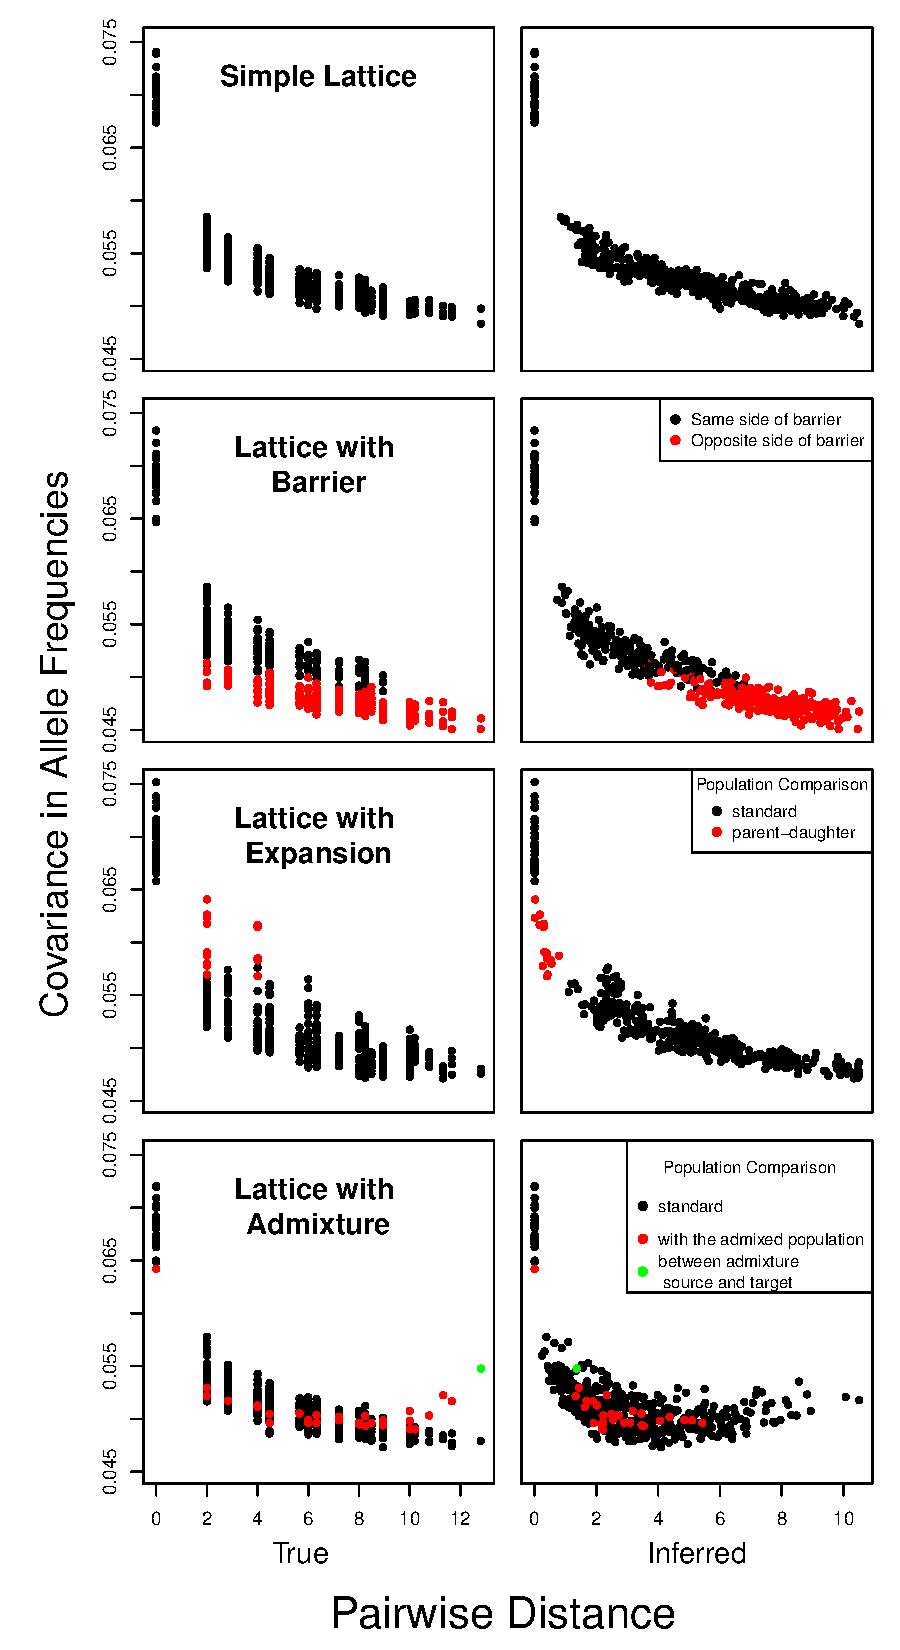
\includegraphics[width=4.8in,height=8.8in]{figs/sims/sim_covariance_decays.pdf}}
		\caption{Decays in covariance for four different simulation scenarios (from top to bottom: simple lattice; lattice with barrier; lattice with expansion; lattice with admixture).  Left column: sample covariance plotted against observed pairwise distance.  Right column: sample covariance plotted against inferred geogenetic distance.}
	\label{sfig:sim_covariance_decays}
\end{figure}


\begin{figure}
\centering
	{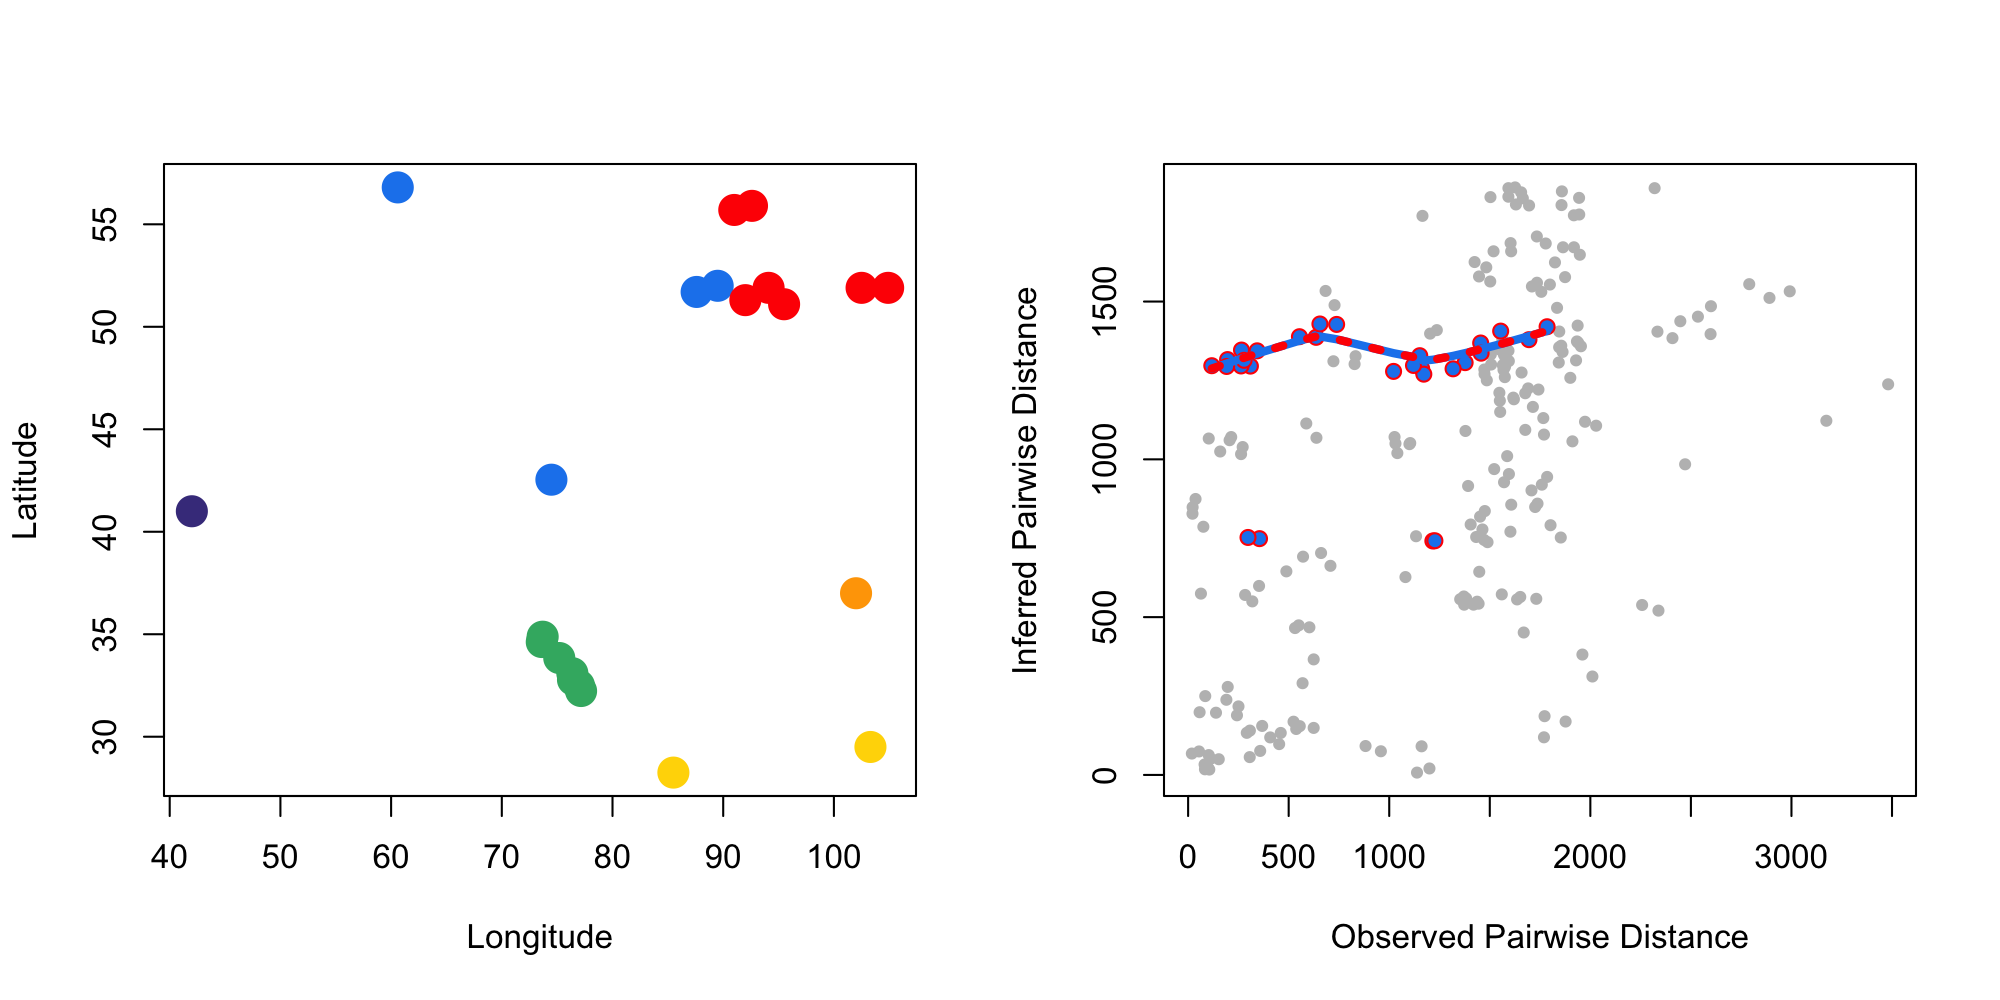
\includegraphics[width=6in,height=2.5in]{figs/warblers/warb_pop_dist_compare.png}}
	\caption{Comparing observed to estimated pairwise distance between warbler populations: a) observed population coordinates; b) observed pairwise distance between populations compared to that between their inferred locations.  The highlighted points show distances between populations from the \textit{plumbeitarsus} and \textit{viridanus} subspecies.  Notice that, regardless of their observed distance, their inferred separations are roughly constant, and much larger than their observed distance.}
	\label{sfig:warb_pop_distcomp}
\end{figure}

\begin{figure}
	\centering
	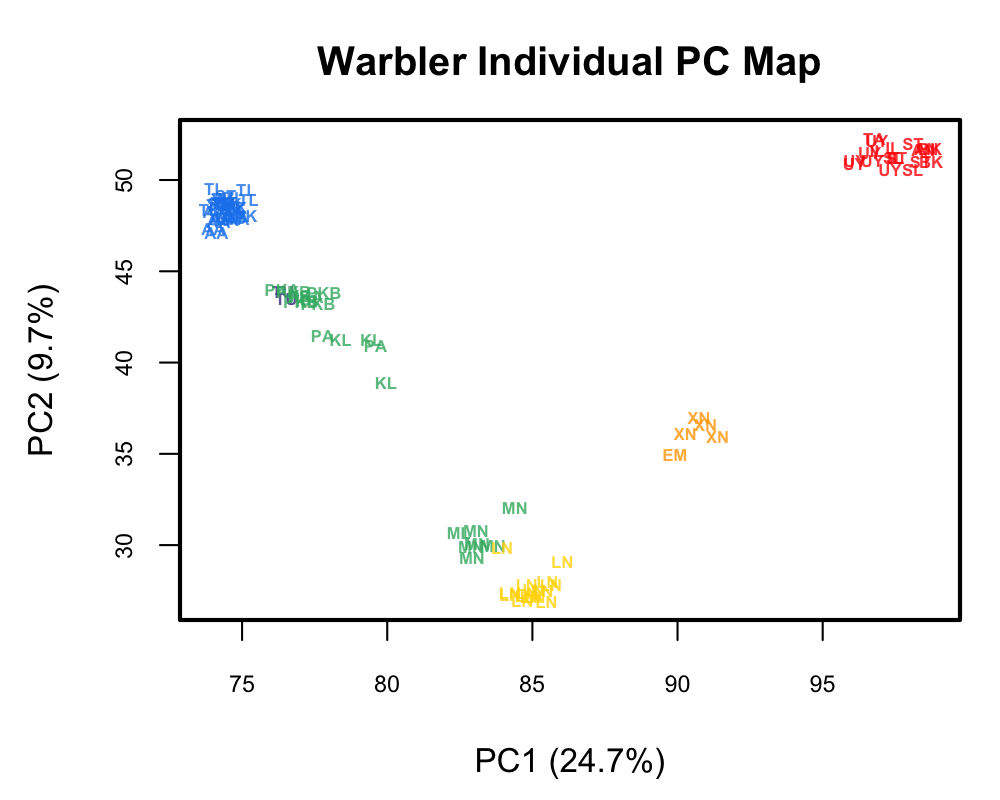
\includegraphics[width=2.4in,height=2in]{figs/warblers/warb_ind_PC_map.png}
	\caption{The map of warbler individuals derived from a Principal Components analysis.}
	\label{sfig:warb_ind_PC_map}
\end{figure}

%\gc{Graham: dont feel like we need the three analyses in main text.} Across the three independent analyses (two with the observed population locations as spatial priors on the locations, $G'$, that they choose for themselves, one with random locations as spatial priors), the inferred values of admixture proportion are consistent (95\% credible intervals:  0.146-0.233, 0.154-0.242, 0.146-0.238).  However, both the position that the Stolby population chooses for itself and the region from which it draws admixture varies between runs (Figure \ref{sfig:warbler_pop_compare}).  In two of the analyses, the Stolby population moves to a position proximate to the \textit{viridanus} cluster and chooses admixture from a point beyond the \textit{plumbeitarsus} cluster, and in one analysis, this pattern is reversed.  

\begin{figure}
	\centering
		\subcaptionbox{\label{warb_pop_realpr1}}
			{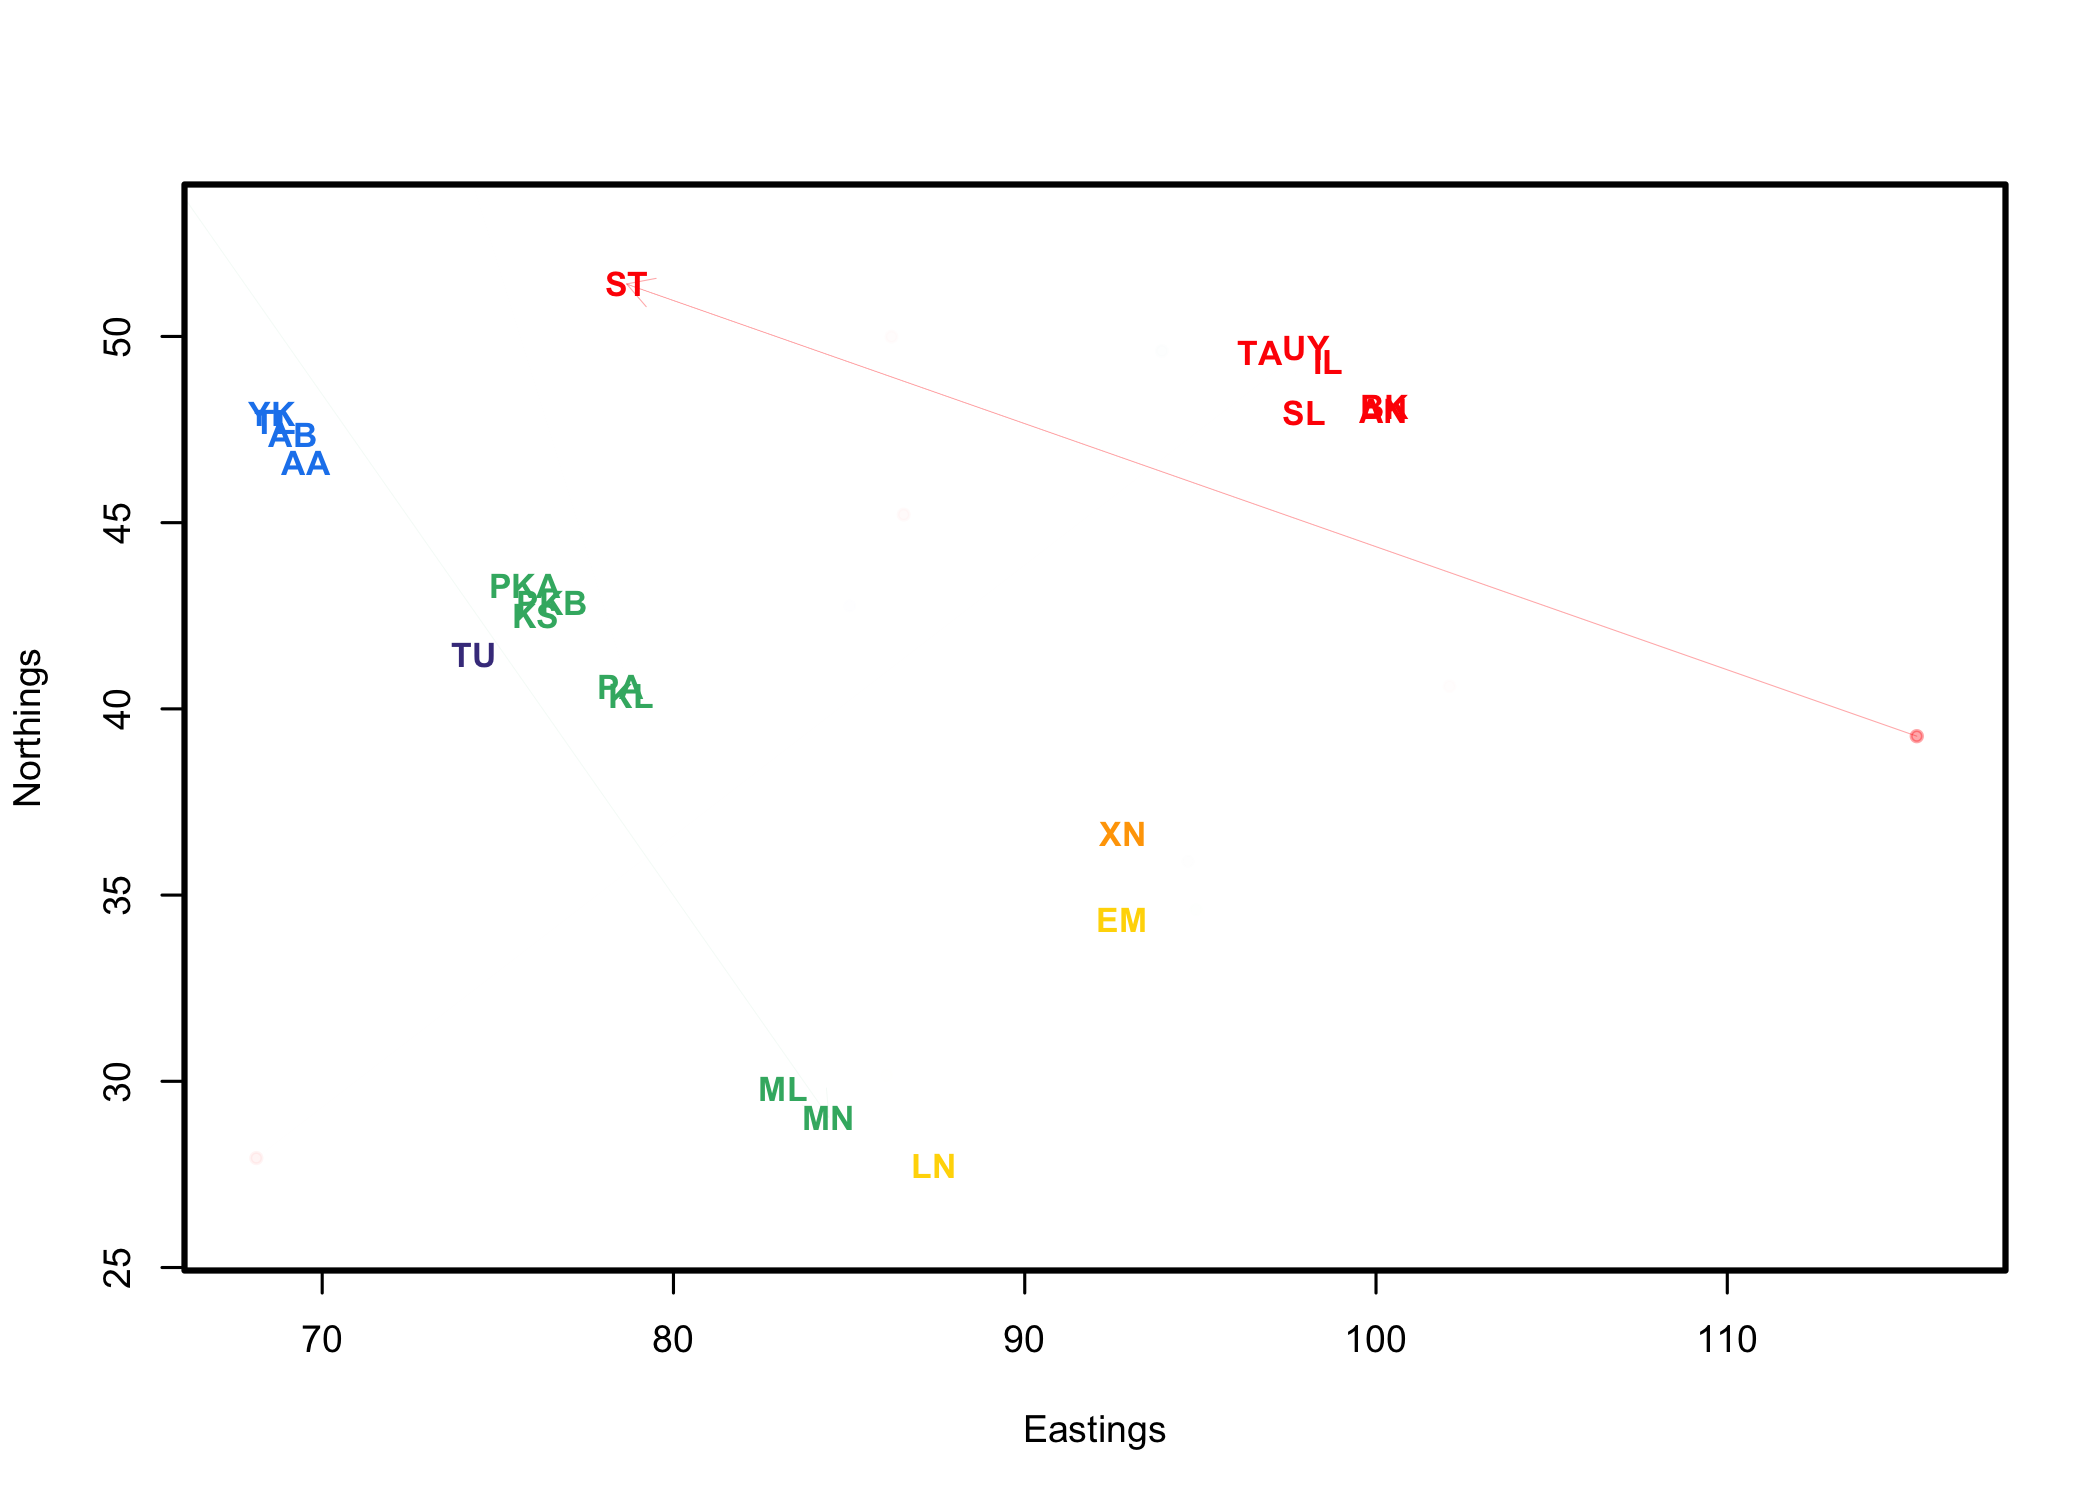
\includegraphics[width=1.85in,height=1.54in]{figs/warblers/population_warbler_map_realpr1.png}}
		\subcaptionbox{\label{warb_pop_realpr2}}			
			{\includegraphics[width=1.85in,height=1.54in]{figs/warblers/population_warbler_map_realpr2.png}}
		\subcaptionbox{\label{warb_pop_randpr1}}
			{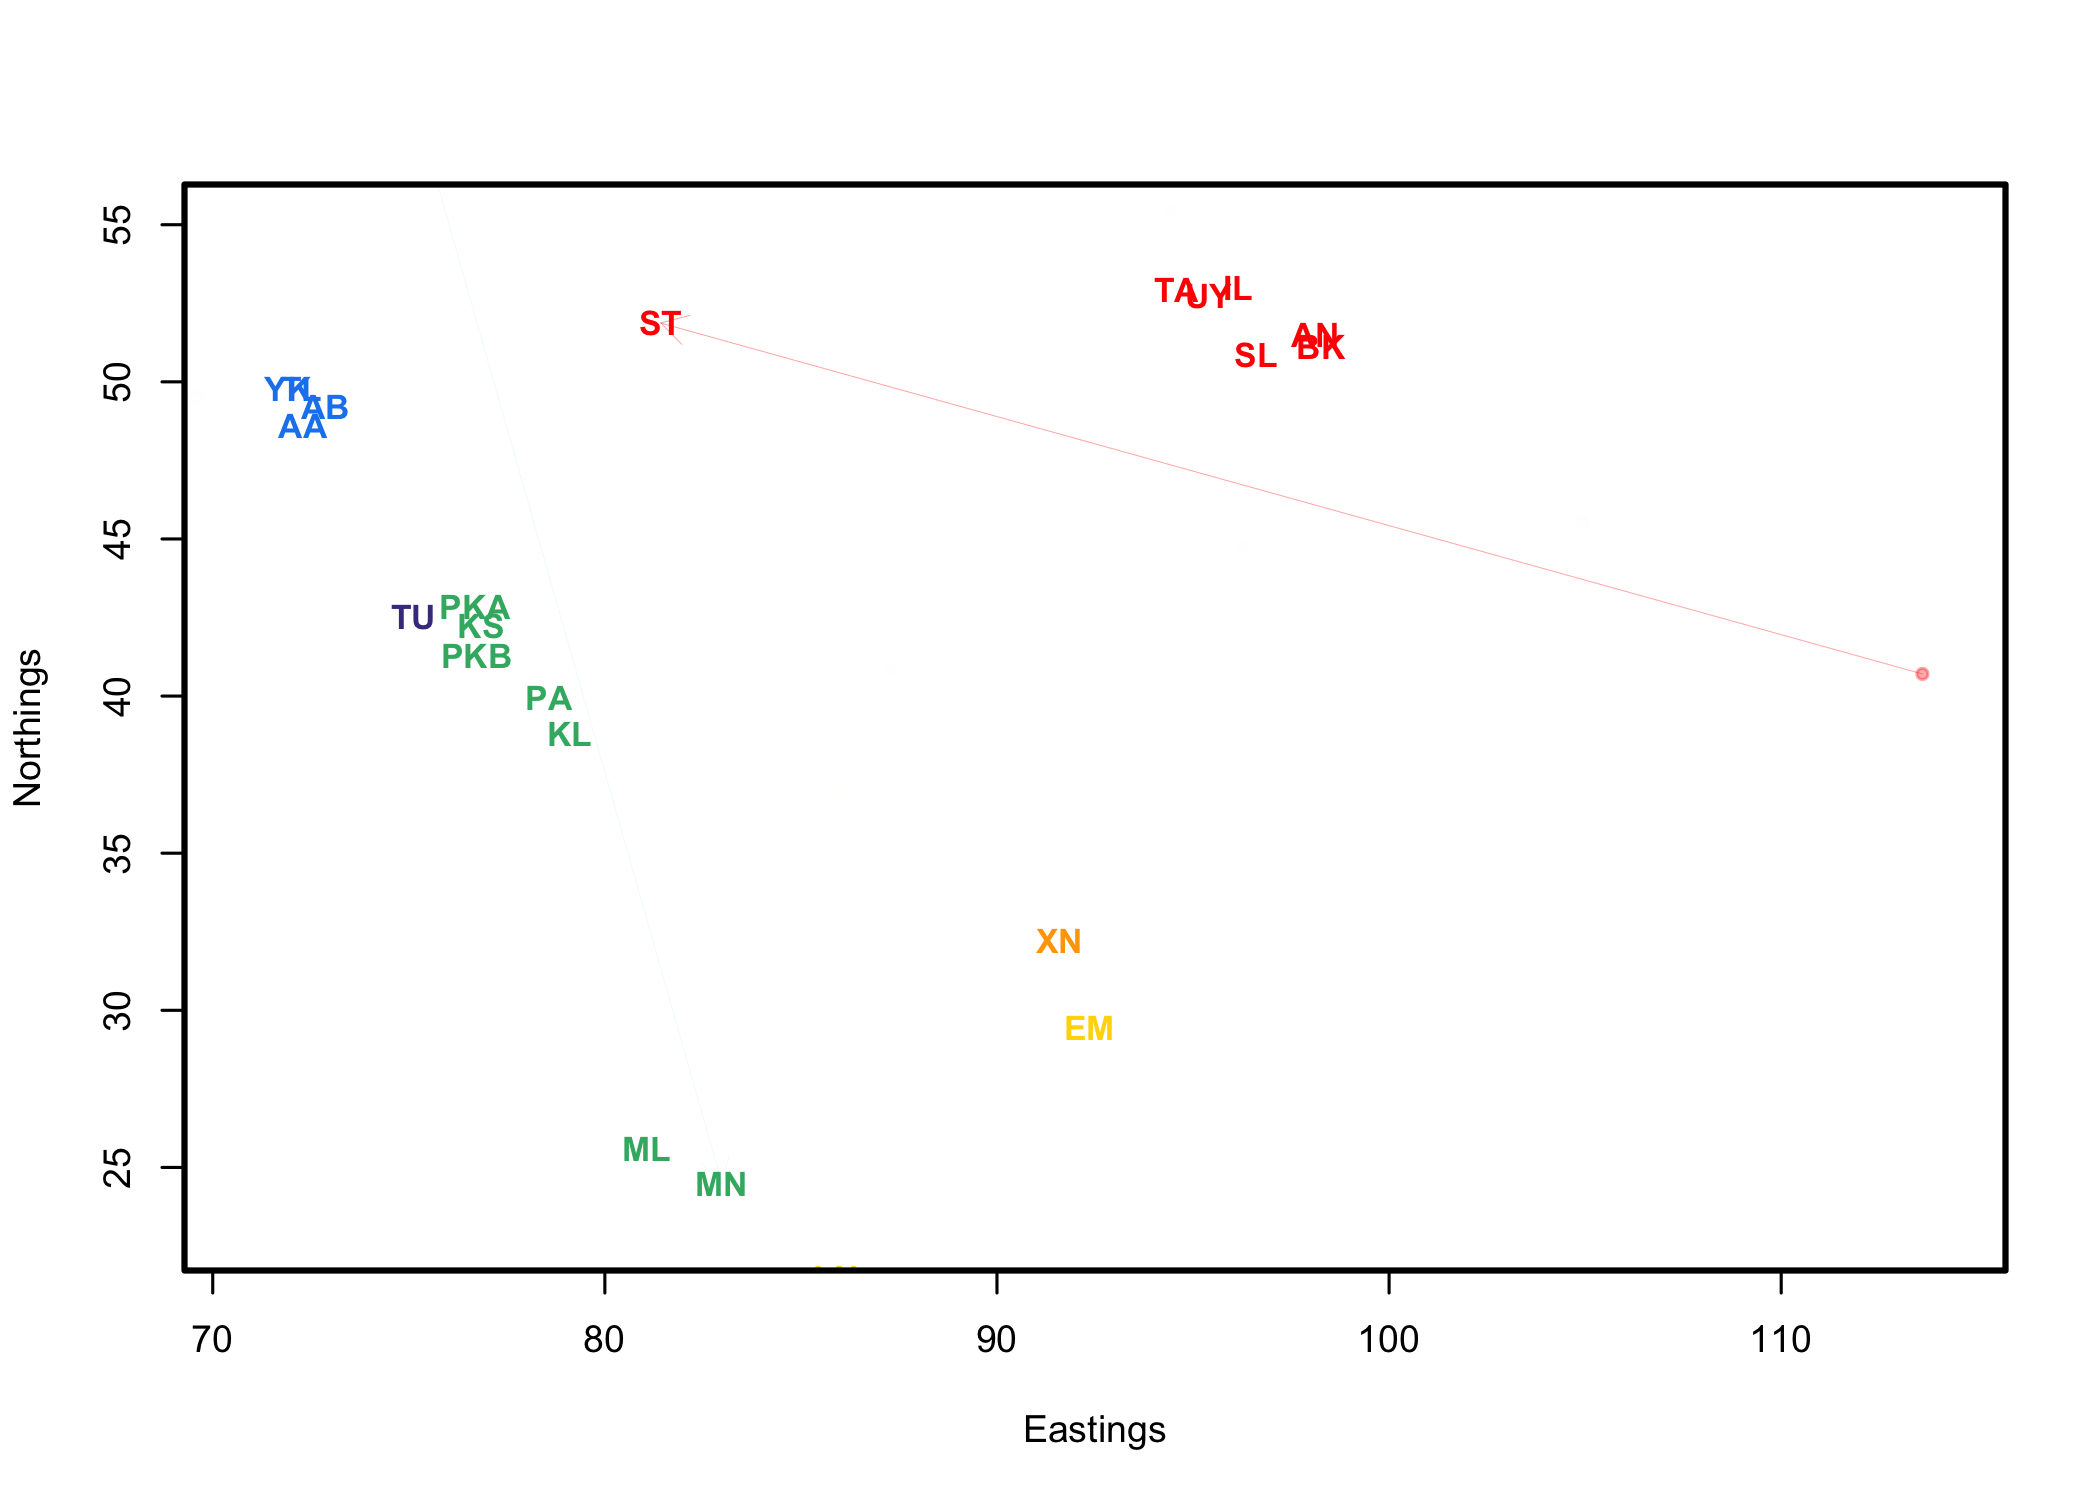
\includegraphics[width=1.85in,height=1.54in]{figs/warblers/population_warbler_map_randpr1.png}}
	\caption{Comparison of inferred maps from three independent analyses.  (a,b) Results from analysis using observed locations as priors on population locations.  (c) Results from analysis using random, uniformly distributed locations within the observed range of latitude and longitude as priors on population locations.}\label{sfig:warbler_pop_compare}
\end{figure}

\begin{figure}
	\centering
		\subcaptionbox{Likelihood \label{admix_prop_func_loc_lnl}}
			{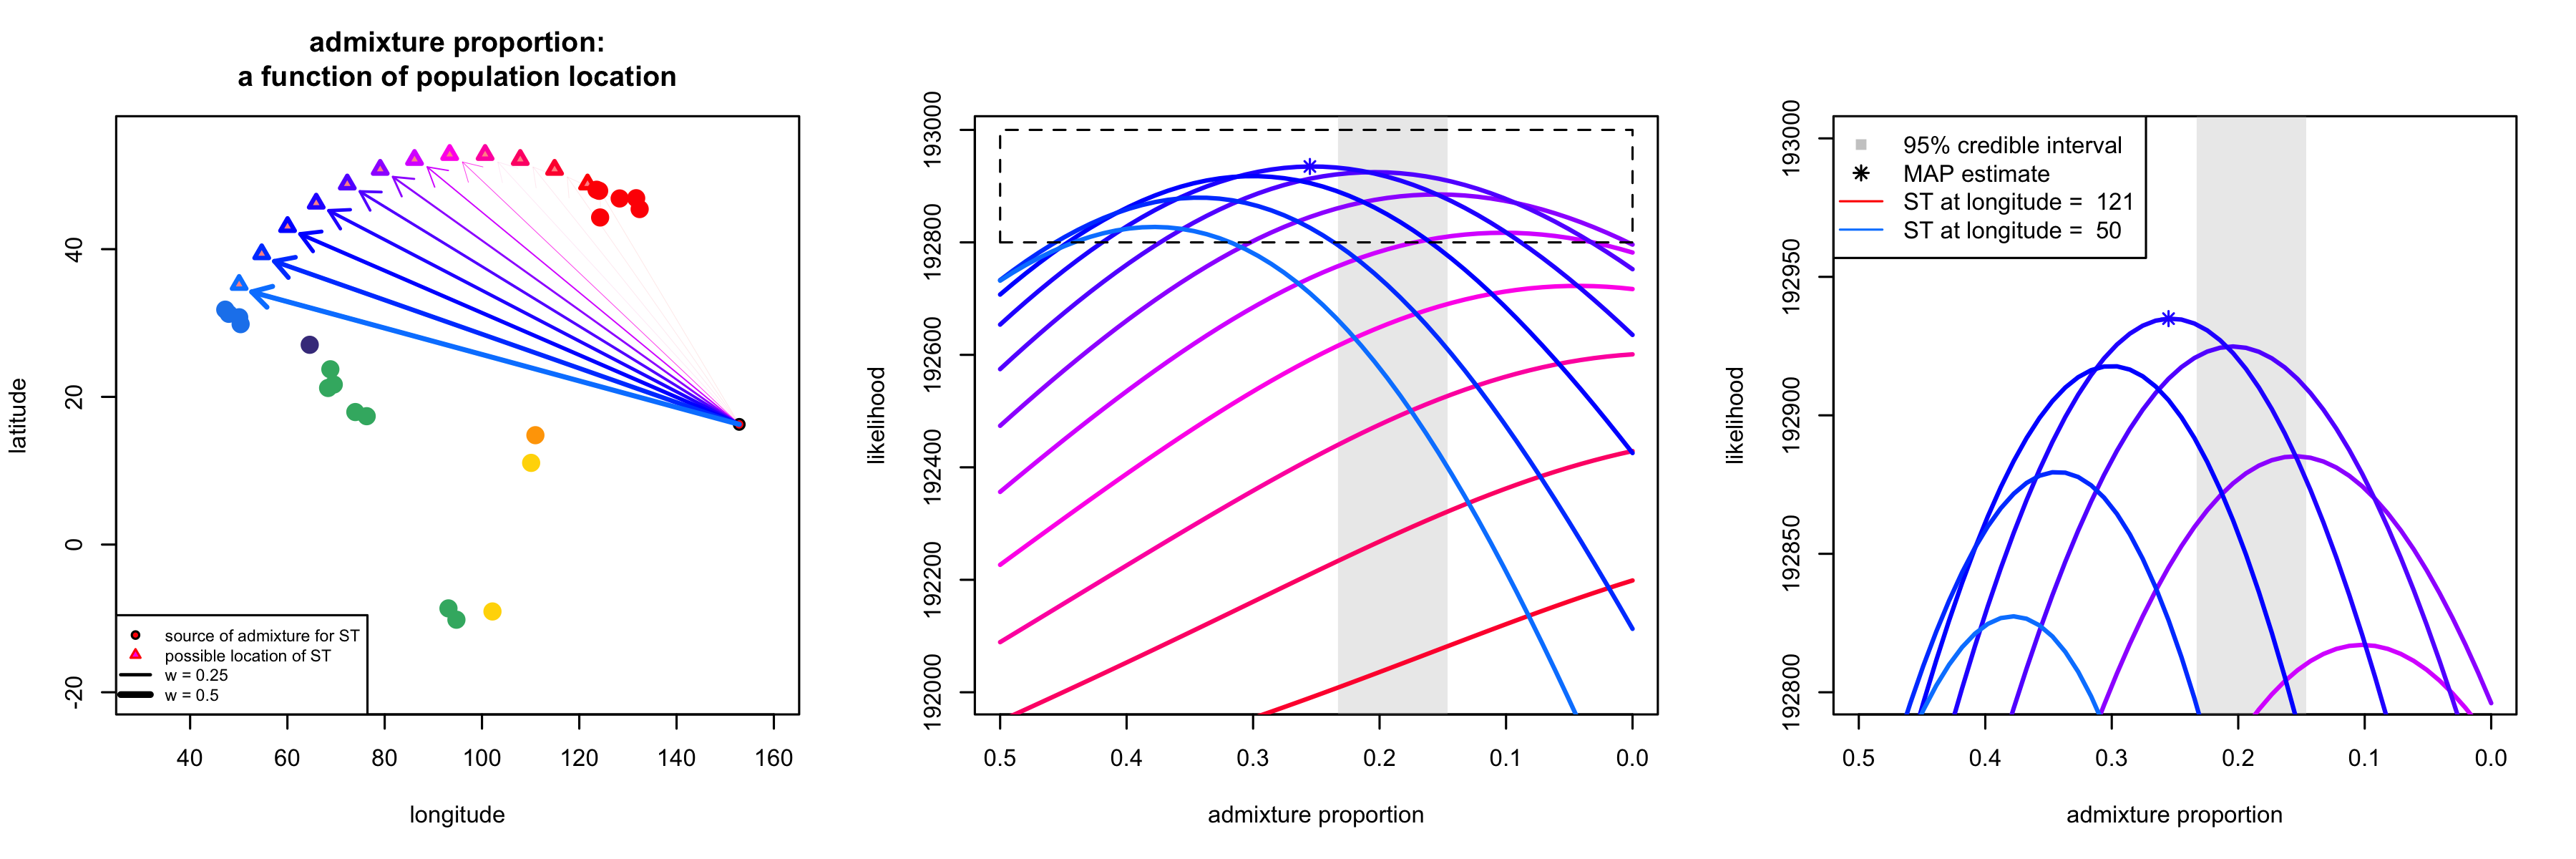
\includegraphics[width=6in,height=2in]{figs/warblers/admix_prop_func_loc_lnl.png}}
		\subcaptionbox{Posterior probability \label{admix_prop_func_loc_prob}}
			{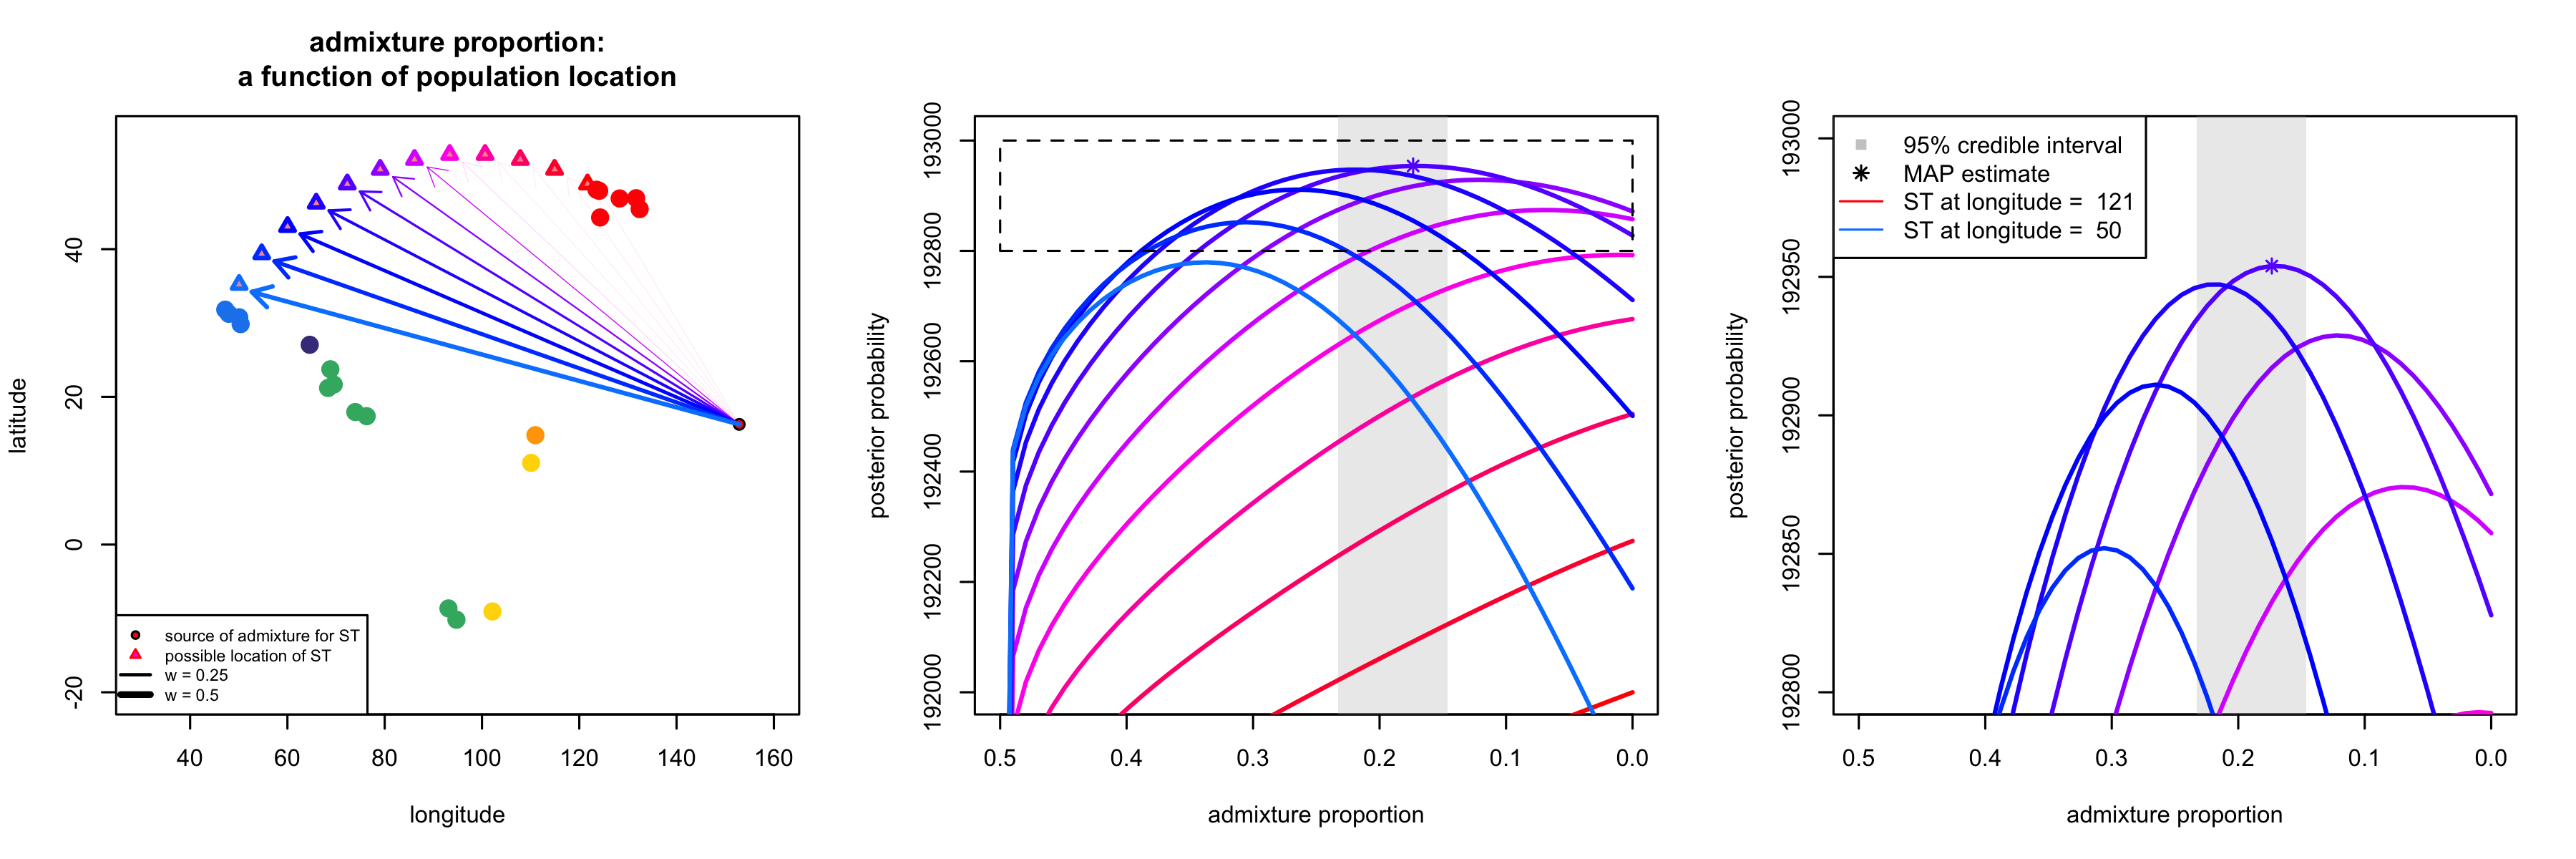
\includegraphics[width=6in,height=2in]{figs/warblers/admix_prop_func_loc_prob.png}}
	\caption{Likelihood surfaces for different placements of population ST between \textit{plumbeitarsus} and \textit{viridanus} clusters: (a) log likelihood surface; (b) posterior probability surface, incorporating the priors.}\label{sfig:admix_prop_func_loc}
\end{figure}

\begin{figure}
	\centering
		\subcaptionbox{All population pairs \label{warb_ind_dist_compare_allpairs}}
			{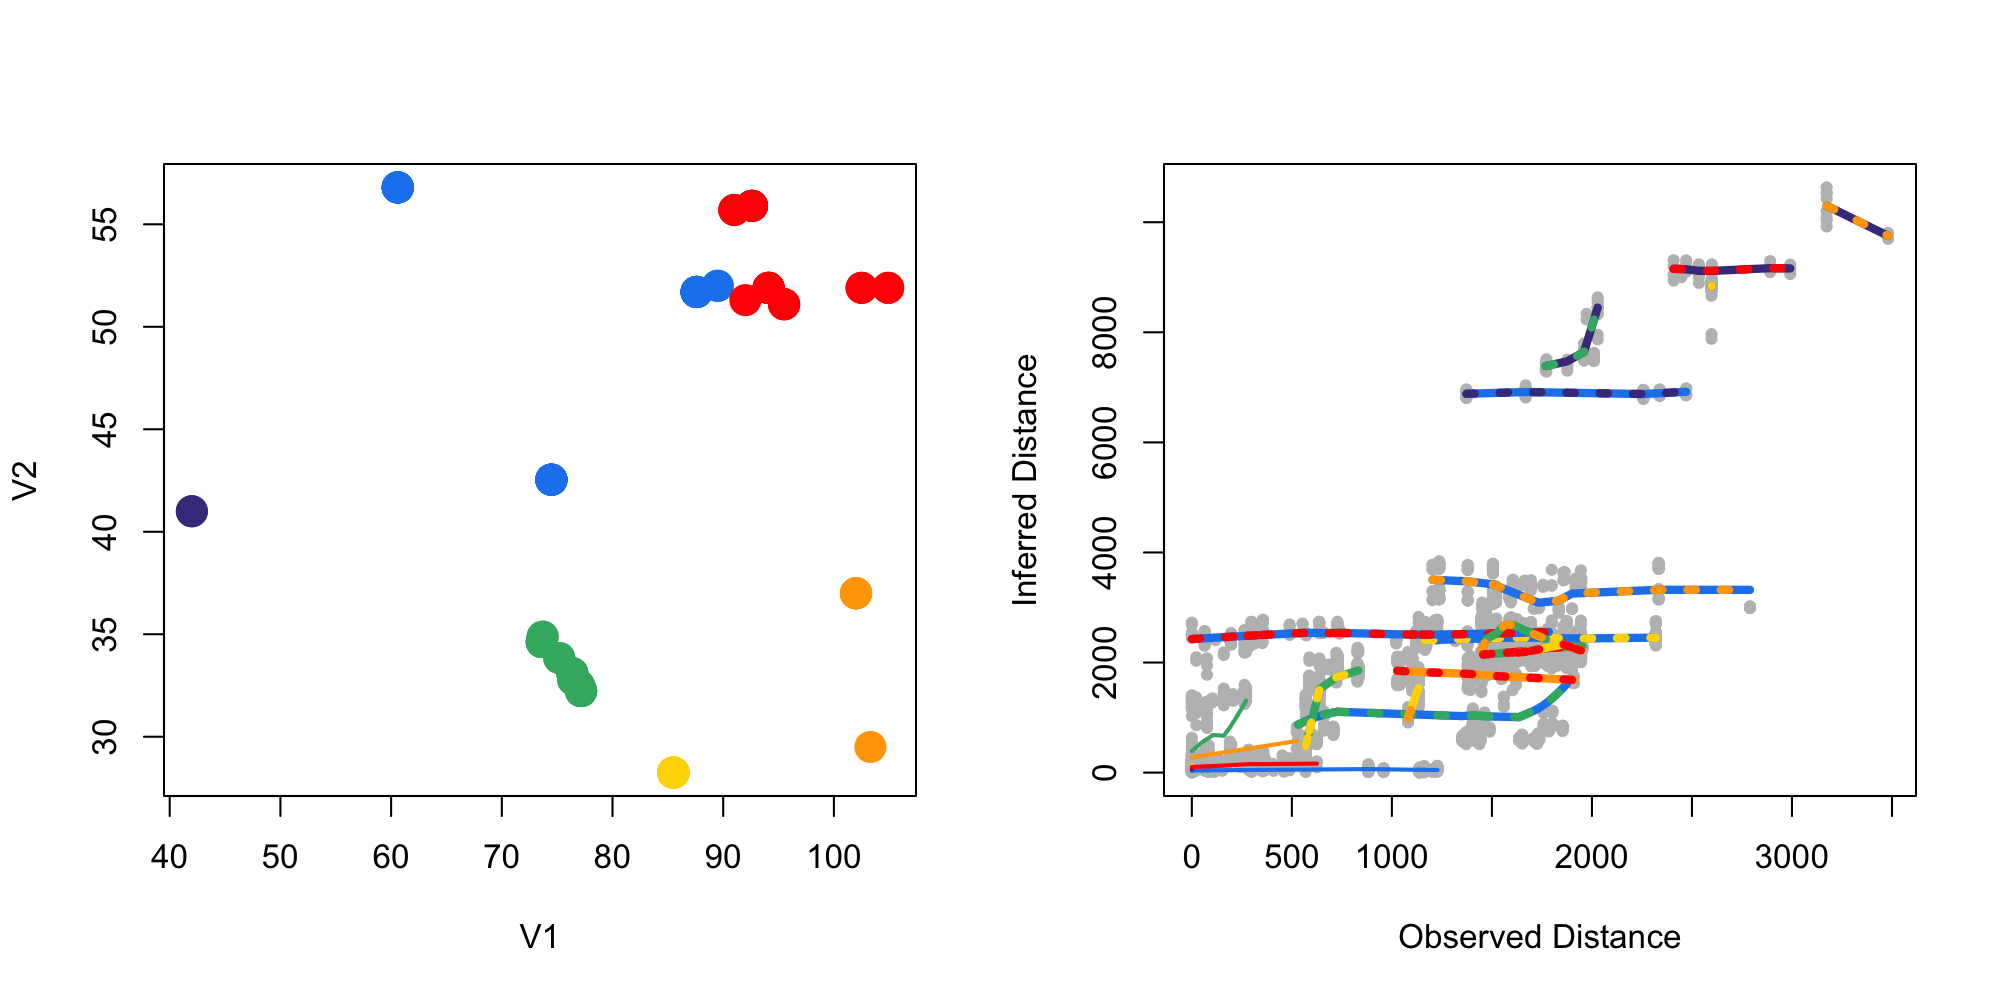
\includegraphics[width=6in,height=3in]{figs/warblers/warb_ind_dist_compare_allpairs.png}}
		\subcaptionbox{Just within population comparisons \label{warb_ind_dist_compare}}
			{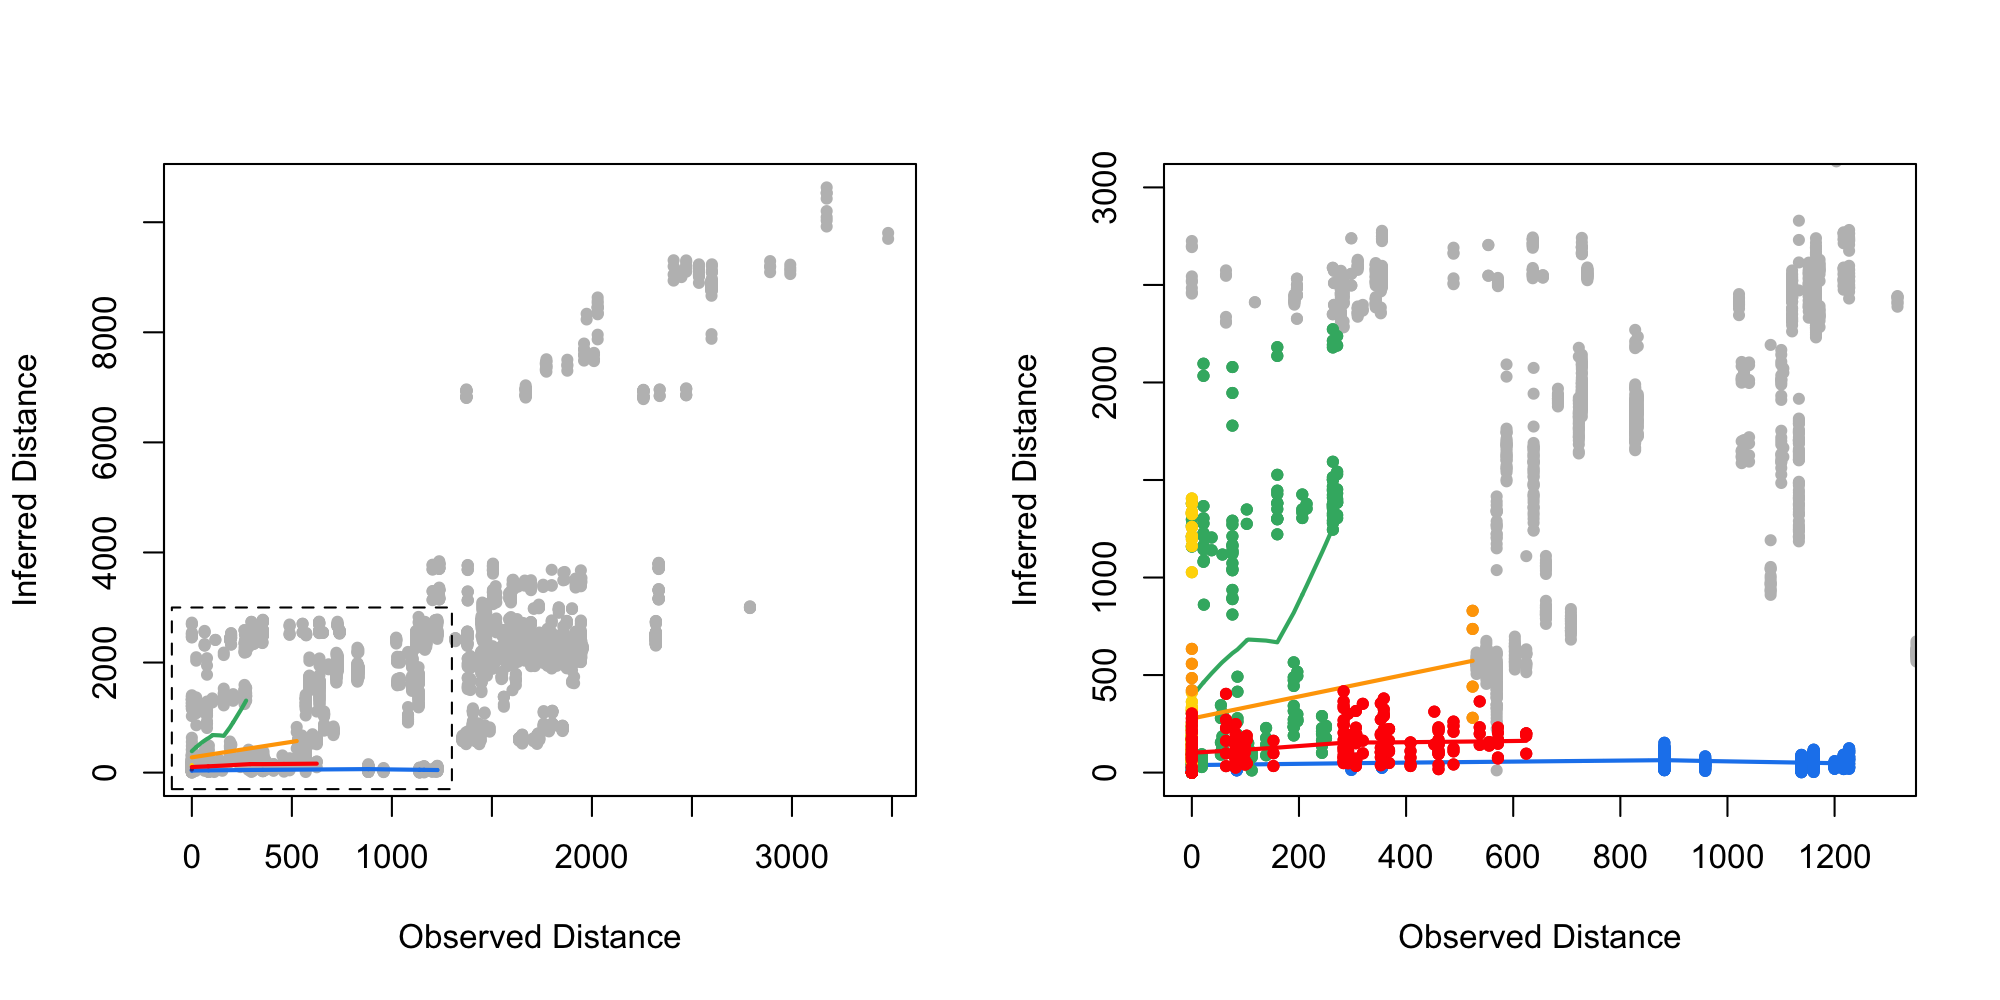
\includegraphics[width=6in,height=3in]{figs/warblers/warb_ind_dist_compare.png}}
	\caption{Comparing observed to estimated pairwise distance between warbler individuals, (a) between and (b) within subspecies populations.}\label{sfig:warb_ind_distcomp}
\end{figure}


\begin{figure}
\centering
	{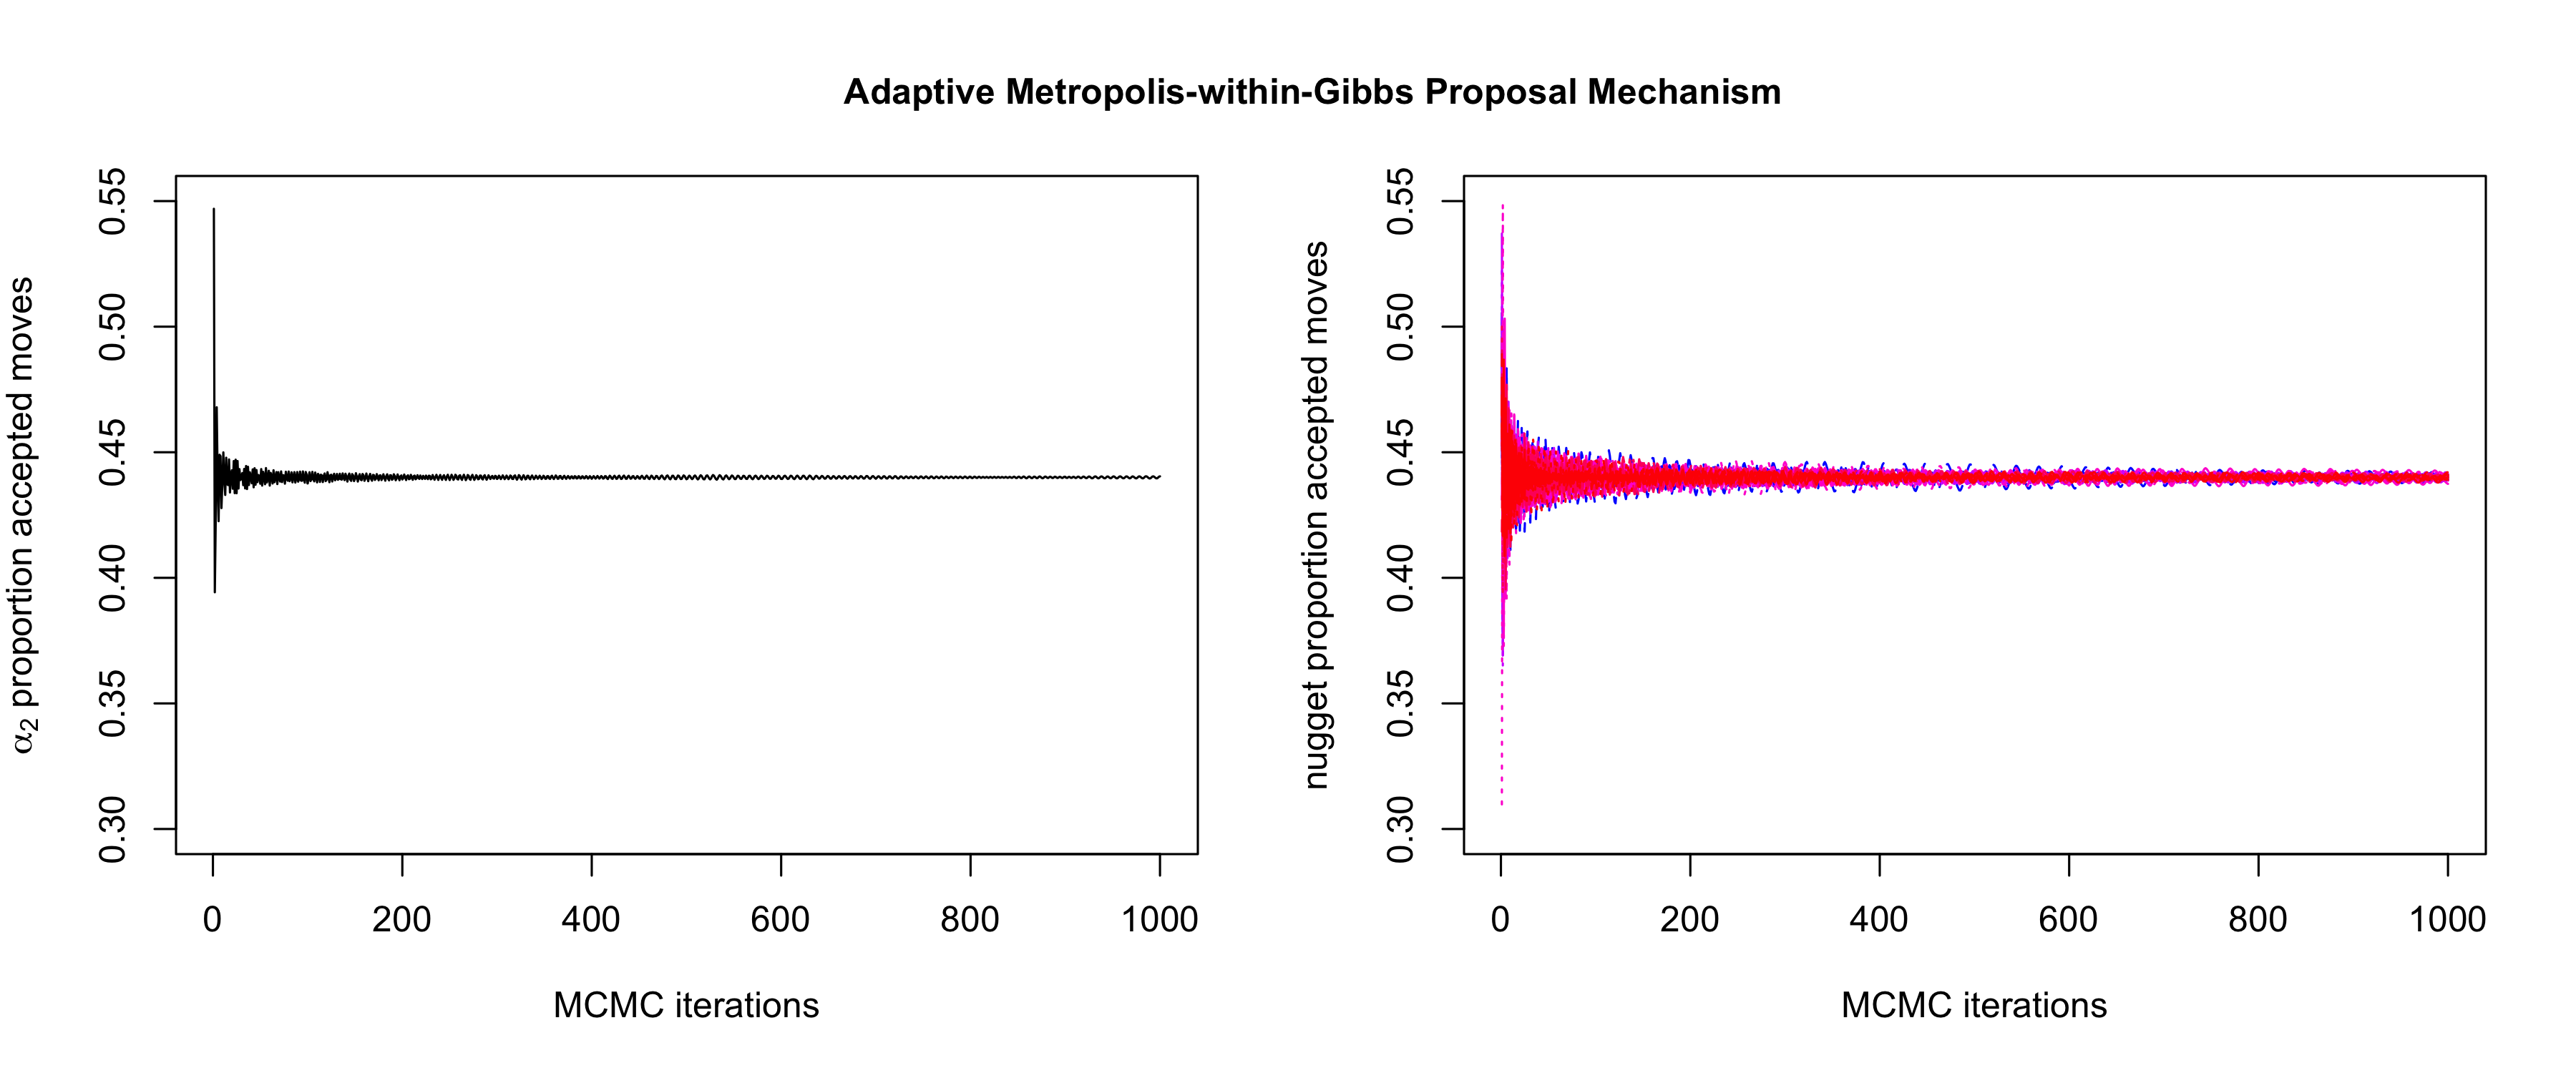
\includegraphics[width=6in,height=2.5in]{figs/sims/example_acceptance_rates.png}}
	\caption{Example parameter acceptance proportions for the $\alpha_2$ parameter and the nugget parameter, $\eta$, using the adaptive Metropolis-within-Gibbs proposal mechanism.}\label{sfig:example_acceptance_rates}
\end{figure}

\begin{figure}
	\centering
		{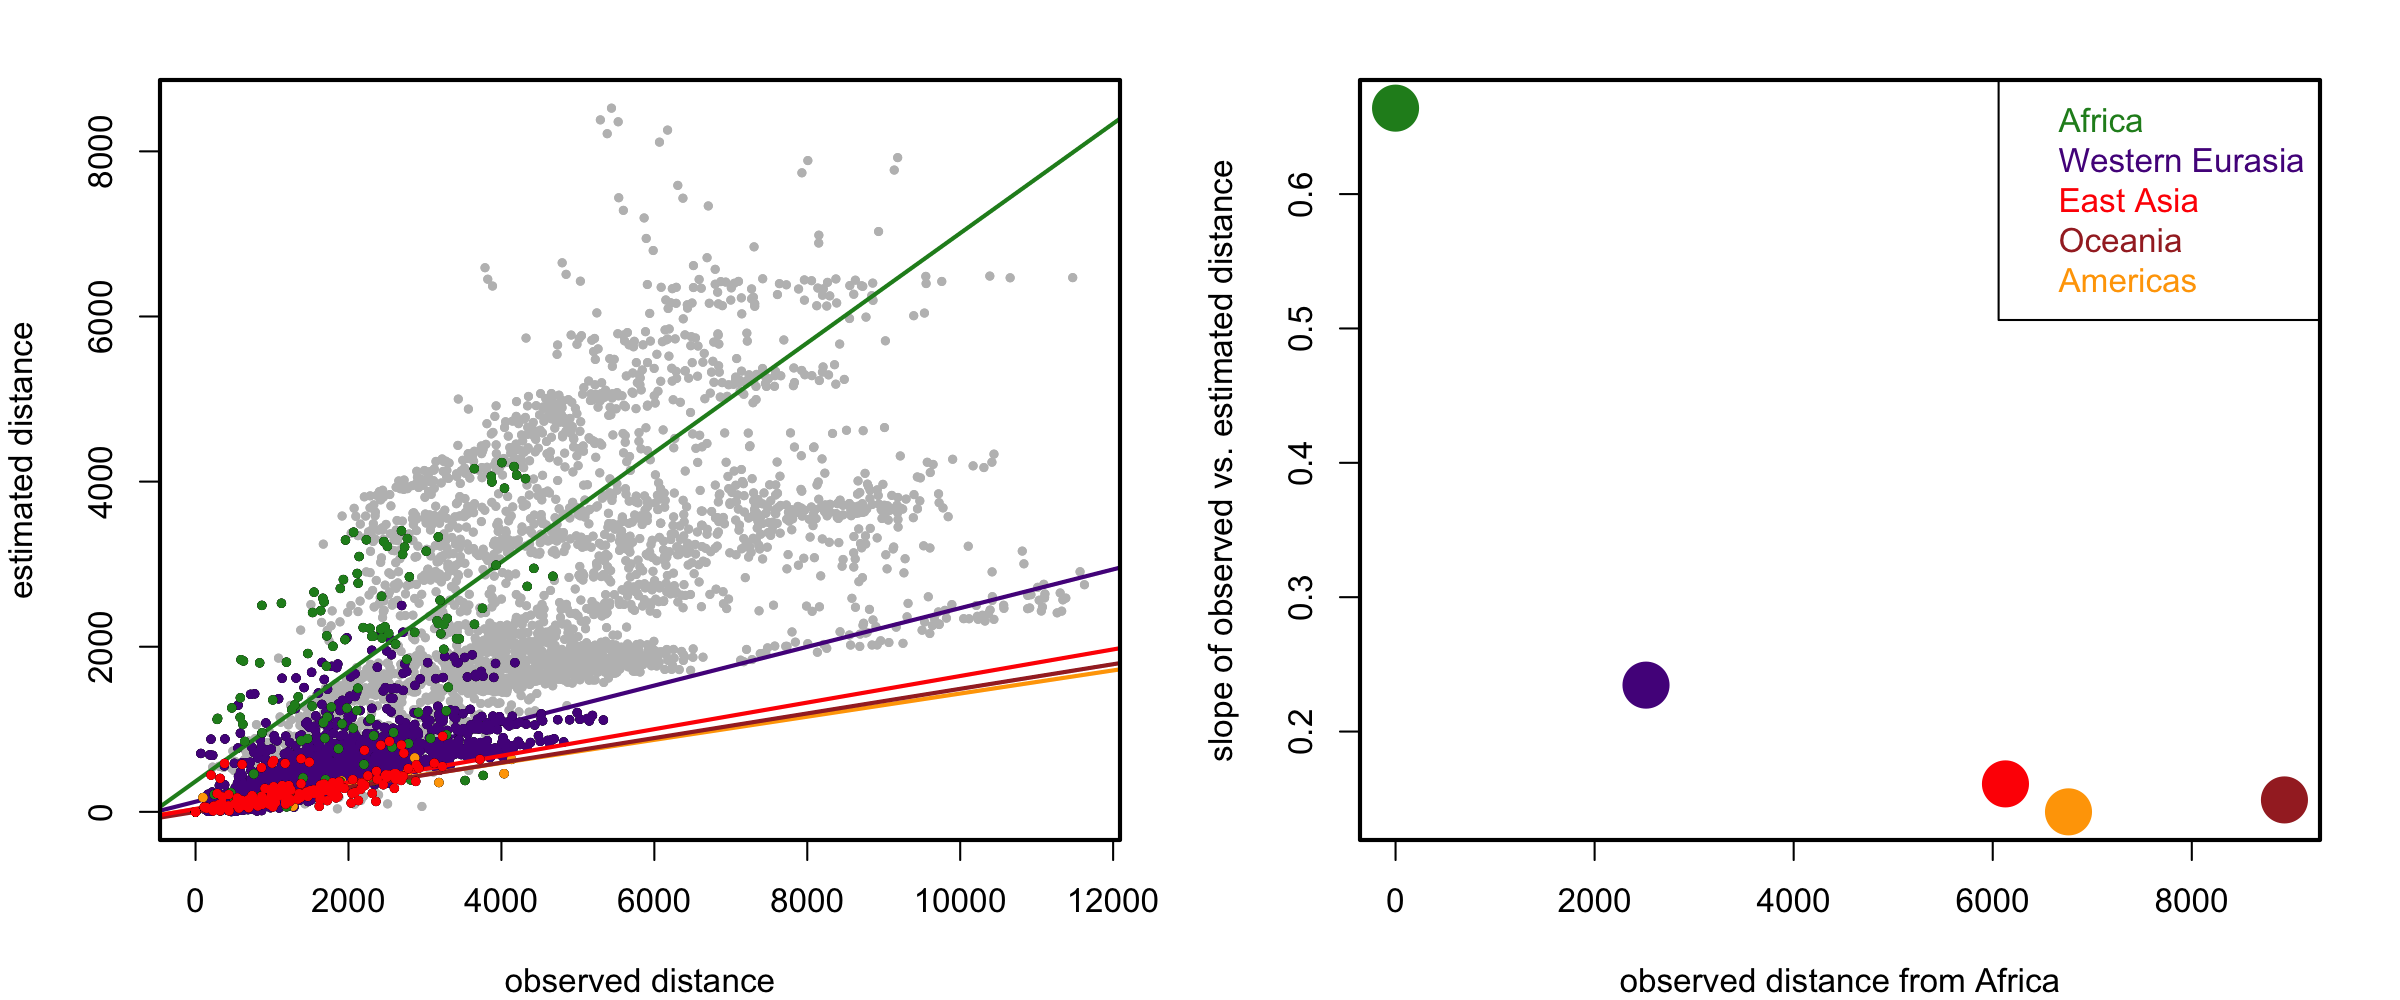
\includegraphics[width=6in,height=2.5in]{figs/globetrotter/globe_NoAd_dist_decay.png}} %globe_NoAd_dist_compare.png
	\caption{Comparison of observed distance to estimated distance between human populations, colored by continent from which populations were sampled (i.e.\ - two populations sampled from Africa are green).  Eurasia is divided into Western Eurasia and East Asia.}
\label{sfig:globe_noad_distcomp}
\end{figure}

\begin{figure}
	\centering
		\subcaptionbox{populations on a line \label{line_scenario}}
			{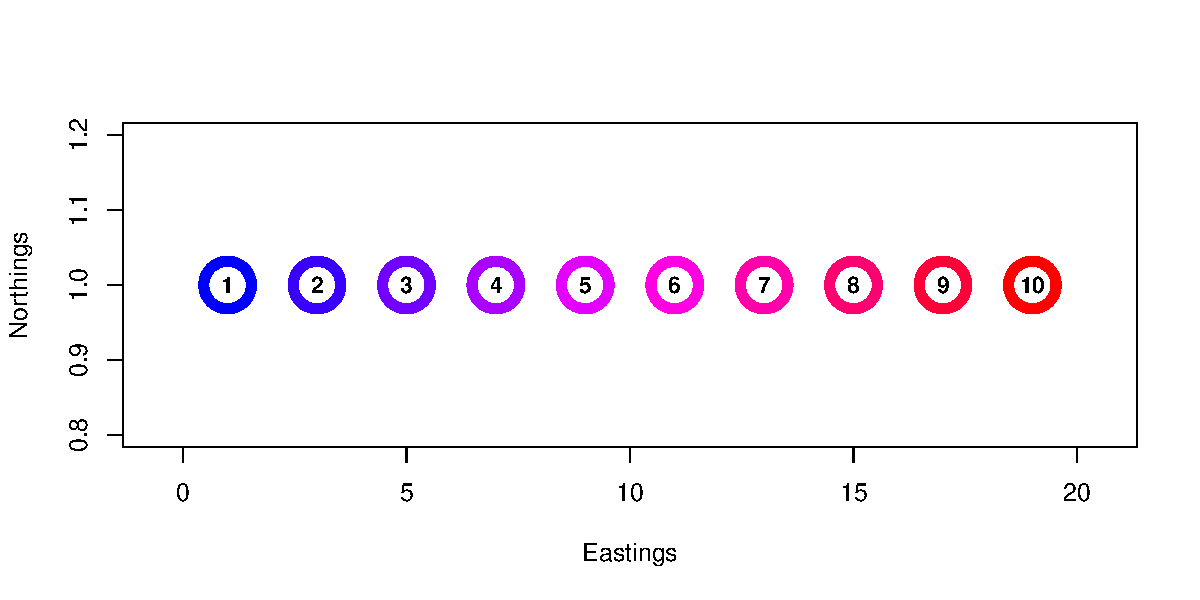
\includegraphics[width=3in,height=1.5in]{figs/sims/line_pops_scenario.pdf}}
		\subcaptionbox{PCA map of line scenario \label{line_pops_pca}}
			{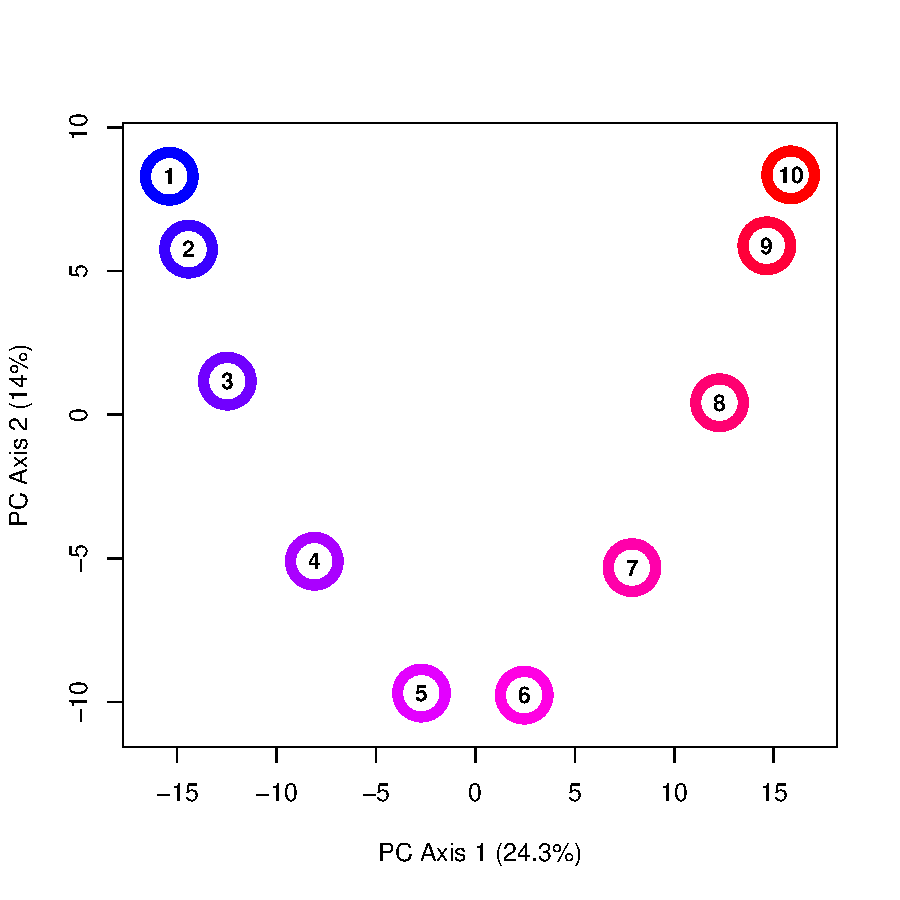
\includegraphics[width=2.33in,height=2.33in]{figs/sims/line_pops_PCA.pdf}}
		\subcaptionbox{posterior from SpaceMix map of line scenario \label{line_pops_post}}
			{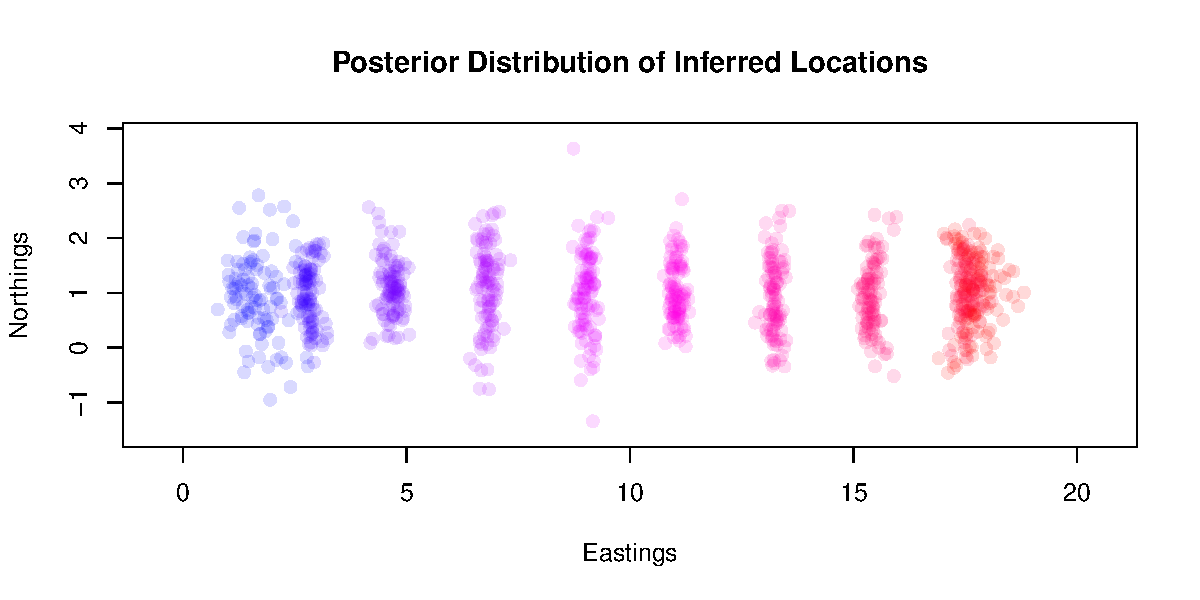
\includegraphics[width=3in,height=1.5in]{figs/sims/line_pops_inference_post.pdf}}
		\subcaptionbox{MAP estimate from SpaceMix map of line scenario \label{line_pops_MAP}}
			{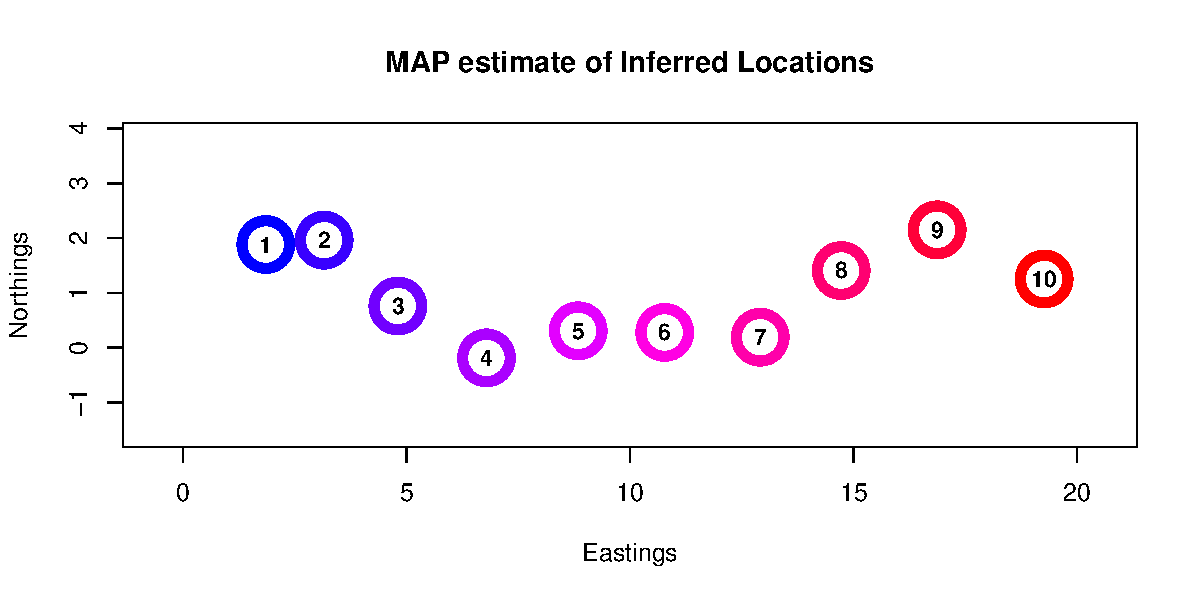
\includegraphics[width=3in,height=1.5in]{figs/sims/line_pops_inference_MAP.pdf}}
	\caption{Simulation scenario of populations on a line, contrasting PCA-based inference and SpaceMix inference. a) Scenario used to simulate data in a spatial coalescent framework with nearest-neighbor migration; b) PCA map of allele frequencies, plotting PC axis 1 against PC axis 2, forming a `U' shape; c) Posterior distribution of SpaceMix location inference, forming a rough line; d) snapshot of the MAP draw from the posterior, again showing a rough line.}
	\label{sfig:line_scenario}
\end{figure}

\begin{figure}
	\centering
		\subcaptionbox{warbler individuals projected onto a line \label{warb_ind_line_setup}}
			{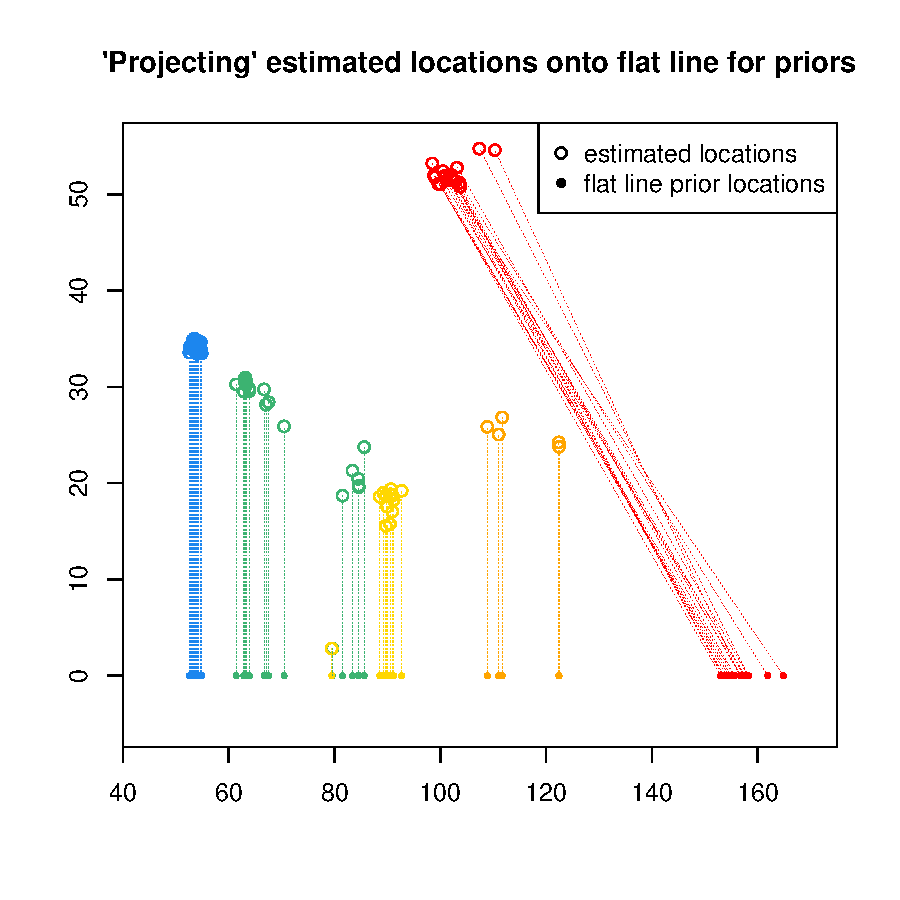
\includegraphics[width=2.8in,height=2.33in]{figs/warblers/warb_inds_on_a_line_setup.pdf}}
		\subcaptionbox{MAP estimate from SpaceMix \label{warb_inds_line_MAP}}
			{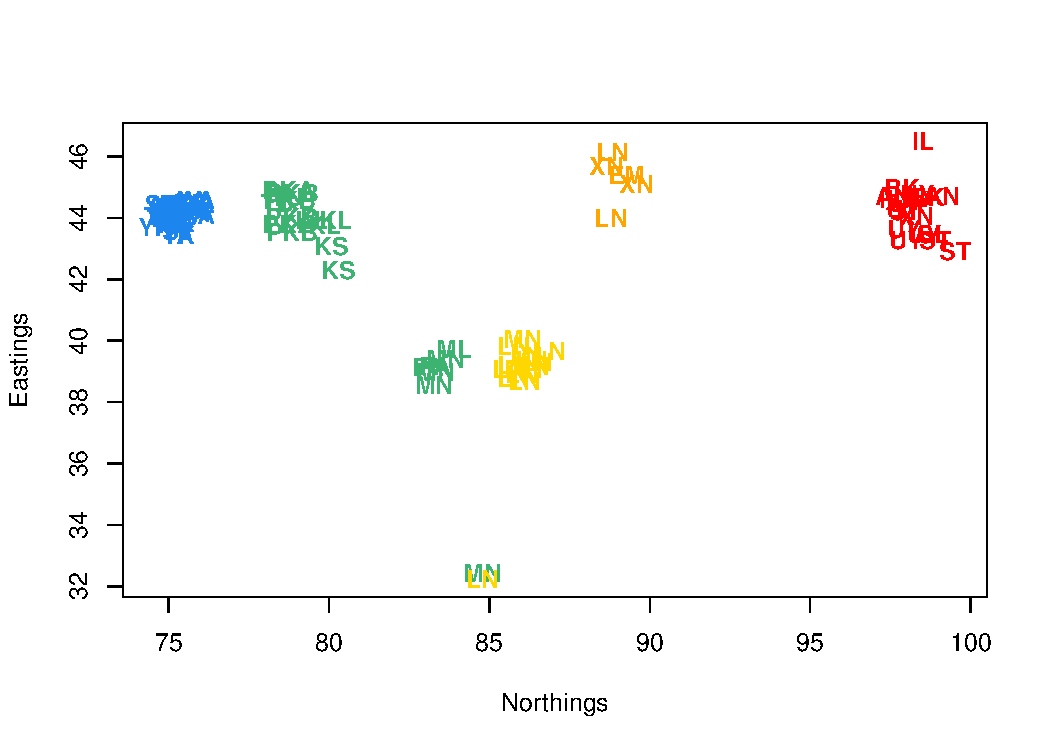
\includegraphics[width=2.8in,height=2.33in]{figs/warblers/warb_inds_on_a_line_MAP1.pdf}}
		\subcaptionbox{Posterior distribution of locations from SpaceMix \label{warb_inds_line_post}}
			{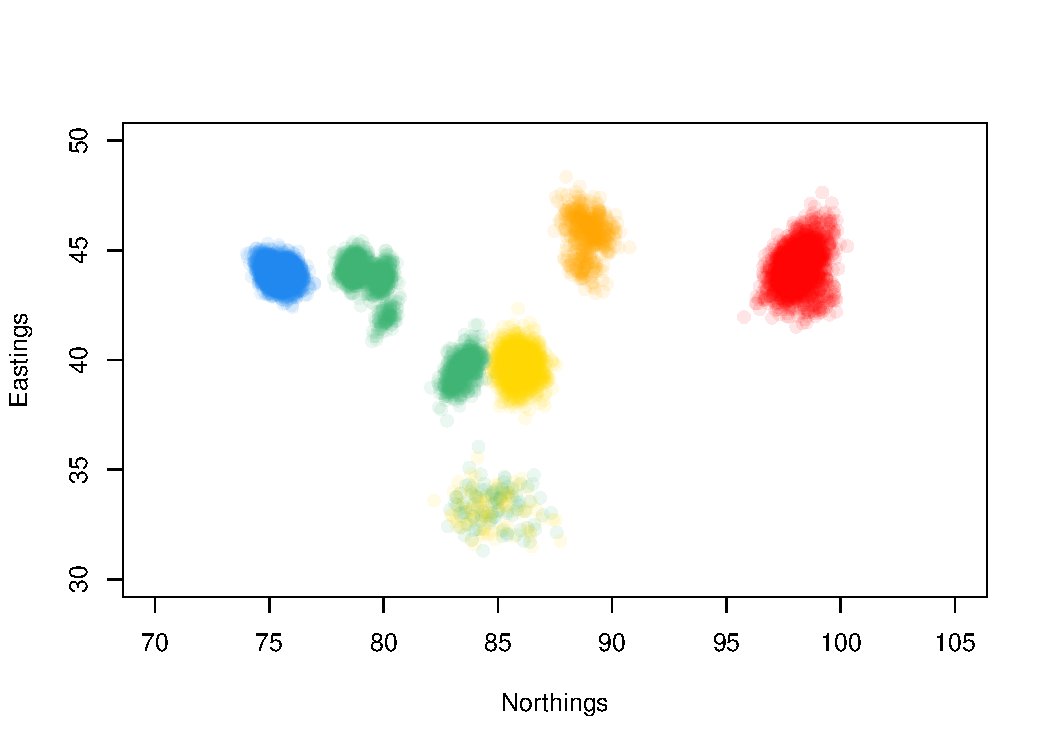
\includegraphics[width=2.8in,height=2.33in]{figs/warblers/warb_inds_on_a_line_post1.pdf}}
	\caption{SpaceMix analyses performed on a warbler individuals for which prior locations are projected onto a flat line in an order that approximately corresponds to their order around the ring: a) the setup of the analysis, in which warbler individuals are projected from their estimated locations in a previous SpaceMix run onto a flat line; b) the MAP estimate of individual locations from a SpaceMix analysis with no admixture, using the flat line locations from (a) as priors on $G^{\prime}$; c) posterior distribution of individual locations from the same analysis.  As with the other inferred maps, here, for clarity, the inferred locations have been rotated via a Procrustes superimposition around their true sampling coordinates.}
	\label{sfig:warb_inds_on_a_line}
\end{figure}

\begin{table}
\centering
\tiny
\begin{tabular}{rlrr}
  \hline
Sample & Subspecies & Longitude & Latitude \\ 
  \hline
 Vir-YK1 & \textcolor{blue}{Viridanus} & 60.60 & 60.60 \\ 
   Vir-YK11 & \textcolor{blue}{Viridanus} & 60.60 & 60.60 \\ 
   Vir-YK3 & \textcolor{blue}{Viridanus} & 60.60 & 60.60 \\ 
   Vir-YK4 & \textcolor{blue}{Viridanus} & 60.60 & 60.60 \\ 
   Vir-YK5 & \textcolor{blue}{Viridanus} & 60.60 & 60.60 \\ 
   Vir-YK6 & \textcolor{blue}{Viridanus} & 60.60 & 60.60 \\ 
   Vir-YK7 & \textcolor{blue}{Viridanus} & 60.60 & 60.60 \\ 
   Vir-YK9 & \textcolor{blue}{Viridanus} & 60.60 & 60.60 \\ 
   Vir-AB1 & \textcolor{blue}{Viridanus} & 89.50 & 89.50 \\ 
   Vir-AB2 & \textcolor{blue}{Viridanus} & 89.50 & 89.50 \\ 
  Vir-STvi1 & \textcolor{blue}{Viridanus} & 92.60 & 92.60 \\ 
  Vir-STvi2 & \textcolor{blue}{Viridanus} & 92.60 & 92.60 \\ 
  Vir-STvi3 & \textcolor{blue}{Viridanus} & 92.60 & 92.60 \\ 
   Vir-TL1 & \textcolor{blue}{Viridanus} & 87.60 & 87.60 \\ 
   Vir-TL10 & \textcolor{blue}{Viridanus} & 87.60 & 87.60 \\ 
   Vir-TL11 & \textcolor{blue}{Viridanus} & 87.60 & 87.60 \\ 
   Vir-TL12 & \textcolor{blue}{Viridanus} & 87.60 & 87.60 \\ 
   Vir-TL2 & \textcolor{blue}{Viridanus} & 87.60 & 87.60 \\ 
   Vir-TL3 & \textcolor{blue}{Viridanus} & 87.60 & 87.60 \\ 
   Vir-TL4 & \textcolor{blue}{Viridanus} & 87.60 & 87.60 \\ 
   Vir-TL5 & \textcolor{blue}{Viridanus} & 87.60 & 87.60 \\ 
   Vir-TL7 & \textcolor{blue}{Viridanus} & 87.60 & 87.60 \\ 
   Vir-TL8 & \textcolor{blue}{Viridanus} & 87.60 & 87.60 \\ 
   Vir-TL9 & \textcolor{blue}{Viridanus} & 87.60 & 87.60 \\ 
   Vir-AA1 & \textcolor{blue}{Viridanus} & 74.48 & 74.48 \\ 
   Vir-AA10 & \textcolor{blue}{Viridanus} & 74.48 & 74.48 \\ 
   Vir-AA11 & \textcolor{blue}{Viridanus} & 74.48 & 74.48 \\ 
   Vir-AA3 & \textcolor{blue}{Viridanus} & 74.48 & 74.48 \\ 
   Vir-AA4 & \textcolor{blue}{Viridanus} & 74.48 & 74.48 \\ 
   Vir-AA5 & \textcolor{blue}{Viridanus} & 74.48 & 74.48 \\ 
   Vir-AA6 & \textcolor{blue}{Viridanus} & 74.48 & 74.48 \\ 
   Vir-AA7 & \textcolor{blue}{Viridanus} & 74.48 & 74.48 \\ 
   Vir-AA8 & \textcolor{blue}{Viridanus} & 74.48 & 74.48 \\ 
   Vir-AA9 & \textcolor{blue}{Viridanus} & 74.48 & 74.48 \\ 
   \hline
   Ni-TU1 & \textcolor{BlueViolet}{Nitidus} & 42.00 & 42.00 \\ 
   Ni-TU2 & \textcolor{BlueViolet}{Nitidus} & 42.00 & 42.00 \\ 
      \hline
   Lud-PKA8 & \textcolor{ForestGreen}{Ludlowi} & 73.69 & 73.69 \\ 
   Lud-PKA10 & \textcolor{ForestGreen}{Ludlowi} & 73.69 & 73.69 \\ 
   Lud-PKB1 & \textcolor{ForestGreen}{Ludlowi} & 73.61 & 73.61 \\ 
   Lud-PKB2 & \textcolor{ForestGreen}{Ludlowi} & 73.61 & 73.61 \\ 
   Lud-PKB4 & \textcolor{ForestGreen}{Ludlowi} & 73.61 & 73.61 \\ 
   Lud-PKB5 & \textcolor{ForestGreen}{Ludlowi} & 73.61 & 73.61 \\ 
   Lud-KS1 & \textcolor{ForestGreen}{Ludlowi} & 75.19 & 75.19 \\ 
   Lud-KS2 & \textcolor{ForestGreen}{Ludlowi} & 75.19 & 75.19 \\ 
   Lud-KL6 & \textcolor{ForestGreen}{Ludlowi} & 76.37 & 76.37 \\ 
   Lud-KL7 & \textcolor{ForestGreen}{Ludlowi} & 76.37 & 76.37 \\ 
   Lud-KL1 & \textcolor{ForestGreen}{Ludlowi} & 76.37 & 76.37 \\ 
   Lud-PA1 & \textcolor{ForestGreen}{Ludlowi} & 76.97 & 76.97 \\ 
   Lud-PA2 & \textcolor{ForestGreen}{Ludlowi} & 76.97 & 76.97 \\ 
   Lud-ML2 & \textcolor{ForestGreen}{Ludlowi} & 76.43 & 76.43 \\ 
   Lud-MN1 & \textcolor{ForestGreen}{Ludlowi} & 77.16 & 77.16 \\ 
   Lud-MN12 & \textcolor{ForestGreen}{Ludlowi} & 77.16 & 77.16 \\ 
   Lud-MN3 & \textcolor{ForestGreen}{Ludlowi} & 77.16 & 77.16 \\ 
   Lud-MN5 & \textcolor{ForestGreen}{Ludlowi} & 77.16 & 77.16 \\ 
   Lud-MN8 & \textcolor{ForestGreen}{Ludlowi} & 77.16 & 77.16 \\ 
   Lud-MN9 & \textcolor{ForestGreen}{Ludlowi} & 77.16 & 77.16 \\ 
      \hline
   Tro-LN1 & \textcolor{Goldenrod}{Trochiloides} & 85.50 & 85.50 \\ 
   Tro-LN10 & \textcolor{Goldenrod}{Trochiloides} & 85.50 & 85.50 \\ 
   Tro-LN11 & \textcolor{Goldenrod}{Trochiloides} & 85.50 & 85.50 \\ 
   Tro-LN12 & \textcolor{Goldenrod}{Trochiloides} & 85.50 & 85.50 \\ 
   Tro-LN14 & \textcolor{Goldenrod}{Trochiloides} & 85.50 & 85.50 \\ 
   Tro-LN16 & \textcolor{Goldenrod}{Trochiloides} & 85.50 & 85.50 \\ 
   Tro-LN18 & \textcolor{Goldenrod}{Trochiloides} & 85.50 & 85.50 \\ 
   Tro-LN19 & \textcolor{Goldenrod}{Trochiloides} & 85.50 & 85.50 \\ 
   Tro-LN2 & \textcolor{Goldenrod}{Trochiloides} & 85.50 & 85.50 \\ 
   Tro-LN20 & \textcolor{Goldenrod}{Trochiloides} & 85.50 & 85.50 \\ 
   Tro-LN3 & \textcolor{Goldenrod}{Trochiloides} & 85.50 & 85.50 \\ 
   Tro-LN4 & \textcolor{Goldenrod}{Trochiloides} & 85.50 & 85.50 \\ 
   Tro-LN6 & \textcolor{Goldenrod}{Trochiloides} & 85.50 & 85.50 \\ 
   Tro-LN7 & \textcolor{Goldenrod}{Trochiloides} & 85.50 & 85.50 \\ 
   Tro-LN8 & \textcolor{Goldenrod}{Trochiloides} & 85.50 & 85.50 \\ 
      \hline
   Obs-EM1 & \textcolor{BurntOrange}{Obscuratus} & 103.30 & 103.30 \\ 
   Obs-XN1 & \textcolor{BurntOrange}{Obscuratus} & 102.00 & 102.00 \\ 
   Obs-XN2 & \textcolor{BurntOrange}{Obscuratus} & 102.00 & 102.00 \\ 
   Obs-XN3 & \textcolor{BurntOrange}{Obscuratus} & 102.00 & 102.00 \\ 
   Obs-XN5 & \textcolor{BurntOrange}{Obscuratus} & 102.00 & 102.00 \\ 
      \hline
   Plu-BK2 & \textcolor{red}{Plumbeitarsus} & 104.90 & 104.90 \\ 
   Plu-BK3 & \textcolor{red}{Plumbeitarsus} & 104.90 & 104.90 \\ 
   Plu-AN1 & \textcolor{red}{Plumbeitarsus} & 102.50 & 102.50 \\ 
   Plu-AN2  & \textcolor{red}{Plumbeitarsus} & 102.50 & 102.50 \\ 
   Plu-IL1 & \textcolor{red}{Plumbeitarsus} & 95.50 & 95.50 \\ 
   Plu-IL2 & \textcolor{red}{Plumbeitarsus} & 95.50 & 95.50 \\ 
   Plu-IL4 & \textcolor{red}{Plumbeitarsus} & 95.50 & 95.50 \\ 
   Plu-ST1 & \textcolor{red}{Plumbeitarsus} & 92.60 & 92.60 \\ 
   Plu-ST12 & \textcolor{red}{Plumbeitarsus} & 92.60 & 92.60 \\ 
   Plu-ST3 & \textcolor{red}{Plumbeitarsus} & 92.60 & 92.60 \\ 
   Plu-UY1 & \textcolor{red}{Plumbeitarsus} & 94.10 & 94.10 \\ 
   Plu-UY2 & \textcolor{red}{Plumbeitarsus} & 94.10 & 94.10 \\ 
   Plu-UY3 & \textcolor{red}{Plumbeitarsus} & 94.10 & 94.10 \\ 
   Plu-UY4 & \textcolor{red}{Plumbeitarsus} & 94.10 & 94.10 \\ 
   Plu-UY5 & \textcolor{red}{Plumbeitarsus} & 94.10 & 94.10 \\ 
   Plu-UY6 & \textcolor{red}{Plumbeitarsus} & 94.10 & 94.10 \\ 
   Plu-SL1 & \textcolor{red}{Plumbeitarsus} & 91.00 & 91.00 \\ 
   Plu-SL2 & \textcolor{red}{Plumbeitarsus} & 91.00 & 91.00 \\ 
   Plu-TA1 & \textcolor{red}{Plumbeitarsus} & 92.00 & 92.00 \\ 
   \hline
   \end{tabular}
   \caption{Subspecies and geographic meta-data for greenish warbler individuals included in analysis}
   \label{tab:warbler_data_table}
\end{table}


 \definecolor{Adygei}{HTML}{4B00FF} 
 \definecolor{Armenian}{HTML}{6200FF} 
 \definecolor{Balochi}{HTML}{B400FF} 
 \definecolor{BantuKenya}{HTML}{00FF12} 
 \definecolor{BantuSouthAfrica}{HTML}{ADFF00} 
 \definecolor{Basque}{HTML}{0047FF} 
 \definecolor{Bedouin}{HTML}{3600FF} 
 \definecolor{Belorussian}{HTML}{2200FF} 
 \definecolor{BiakaPygmy}{HTML}{00FF72} 
 \definecolor{Brahui}{HTML}{AD00FF} 
 \definecolor{Bulgarian}{HTML}{1800FF} 
 \definecolor{Burusho}{HTML}{CE00FF} 
 \definecolor{Cambodian}{HTML}{FF00BC} 
 \definecolor{Chuvash}{HTML}{7500FF} 
 \definecolor{Colombian}{HTML}{FF9800} 
 \definecolor{Cypriot}{HTML}{3600FF} 
 \definecolor{Dai}{HTML}{FF00D2} 
 \definecolor{Daur}{HTML}{FF0074} 
 \definecolor{Druze}{HTML}{4300FF} 
 \definecolor{EastSicilian}{HTML}{000BFF} 
 \definecolor{Egyptian}{HTML}{006CFF} 
 \definecolor{English}{HTML}{004AFF} 
 \definecolor{Ethiopian}{HTML}{00FCFF} 
 \definecolor{EthiopianJew}{HTML}{009CFF} 
 \definecolor{Finnish}{HTML}{1900FF} 
 \definecolor{French}{HTML}{0040FF} 
 \definecolor{Georgian}{HTML}{6000FF} 
 \definecolor{GermanyAustria}{HTML}{0020FF} 
 \definecolor{Greek}{HTML}{0A00FF} 
 \definecolor{Hadza}{HTML}{1EFF00} 
 \definecolor{Han}{HTML}{FF009A} 
 \definecolor{HanNchina}{HTML}{FF00B0} 
 \definecolor{Hazara}{HTML}{BD00FF} 
 \definecolor{Hezhen}{HTML}{FF0053} 
 \definecolor{Hungarian}{HTML}{0200FF} 
 \definecolor{IndianJew}{HTML}{CA00FF} 
 \definecolor{Indian}{HTML}{DC00FF} 
 \definecolor{Myanmar}{HTML}{FF00DD} 
 \definecolor{Iranian}{HTML}{8200FF} 
 \definecolor{Ireland}{HTML}{0066FF} 
 \definecolor{Japanese}{HTML}{FF0040} 
 \definecolor{Jordanian}{HTML}{4300FF} 
 \definecolor{Kalash}{HTML}{C300FF} 
 \definecolor{Karitiana}{HTML}{FFA600} 
 \definecolor{Lahu}{HTML}{FF00CA} 
 \definecolor{Lezgin}{HTML}{6B00FF} 
 \definecolor{Lithuanian}{HTML}{1200FF} 
 \definecolor{Makrani}{HTML}{A900FF} 
 \definecolor{Mandenka}{HTML}{00CCFF} 
 \definecolor{Maya}{HTML}{FF5B00} 
 \definecolor{MbutiPygmy}{HTML}{00FF42} 
 \definecolor{Melanesian}{HTML}{FF0000} 
 \definecolor{Miao}{HTML}{FF00B0} 
 \definecolor{Mongola}{HTML}{FF0087} 
 \definecolor{Moroccan}{HTML}{000CFF} 
 \definecolor{Mozabite}{HTML}{003CFF} 
 \definecolor{Naxi}{HTML}{FF00CE} 
 \definecolor{NorthItalian}{HTML}{0023FF} 
 \definecolor{Norwegian}{HTML}{0027FF} 
 \definecolor{Orcadian}{HTML}{0053FF} 
 \definecolor{Oroqen}{HTML}{FF006D} 
 \definecolor{Palestinian}{HTML}{3C00FF} 
 \definecolor{Papuan}{HTML}{FF002D} 
 \definecolor{Pathan}{HTML}{C900FF} 
 \definecolor{Pima}{HTML}{FF2E00} 
 \definecolor{Polish}{HTML}{0000FF} 
 \definecolor{Romanian}{HTML}{1600FF} 
 \definecolor{Russian}{HTML}{4F00FF} 
 \definecolor{Sandawe}{HTML}{00FFA2} 
 \definecolor{SanNamibia}{HTML}{4EFF00} 
 \definecolor{SanKhomani}{HTML}{7DFF00} 
 \definecolor{Sardinian}{HTML}{0026FF} 
 \definecolor{Saudi}{HTML}{6200FF} 
 \definecolor{Scottish}{HTML}{0057FF} 
 \definecolor{She}{HTML}{FF0087} 
 \definecolor{Sindhi}{HTML}{BC00FF} 
 \definecolor{SouthItalian}{HTML}{0008FF} 
 \definecolor{Spanish}{HTML}{0055FF} 
 \definecolor{Surui}{HTML}{FFA800} 
 \definecolor{Syrian}{HTML}{4B00FF} 
 \definecolor{Tu}{HTML}{FF00CA} 
 \definecolor{Tujia}{HTML}{FF00A9} 
 \definecolor{Tunisian}{HTML}{2400FF} 
 \definecolor{Turkish}{HTML}{3D00FF} 
 \definecolor{Tuscan}{HTML}{001EFF} 
 \definecolor{UAE}{HTML}{8500FF} 
 \definecolor{Uygur}{HTML}{E900FF} 
 \definecolor{Uzbekistani}{HTML}{AB00FF} 
 \definecolor{Welsh}{HTML}{0055FF} 
 \definecolor{WestSicilian}{HTML}{0018FF} 
 \definecolor{Xibo}{HTML}{E900FF} 
 \definecolor{Yakut}{HTML}{FF0062} 
 \definecolor{Yemeni}{HTML}{6F00FF} 
 \definecolor{Yi}{HTML}{FF00C3} 
 \definecolor{Yoruba}{HTML}{00FFD2}
 
 
 \begin{table}[ht]
 \tiny
\centering
\begin{tabular}{rlrrr}
  \hline
 & Population & Longitude & Latitude & Mean Sample Size \\ 
  \hline
1 & \textcolor{BantuSouthAfrica}{BantuSouthAfrica} & 28.00 & -26.00 & 15.99 \\ 
  2 & \textcolor{SanKhomani}{SanKhomani} & 18.10 & -24.60 & 59.96 \\ 
  3 & \textcolor{SanNamibia}{SanNamibia} & 20.00 & -21.50 & 9.99 \\ 
  4 & \textcolor{Hadza}{Hadza} & 33.10 & -4.50 & 5.93 \\ 
  5 & \textcolor{BantuKenya}{BantuKenya} & 37.00 & -3.00 & 21.99 \\ 
  6 & \textcolor{MbutiPygmy}{MbutiPygmy} & 29.00 & 1.00 & 25.98 \\ 
  7 & \textcolor{BiakaPygmy}{BiakaPygmy} & 17.00 & 4.00 & 41.97 \\ 
  8 & \textcolor{Sandawe}{Sandawe} & 35.70 & 6.20 & 55.94 \\ 
  9 & \textcolor{Yoruba}{Yoruba} & 5.00 & 8.00 & 41.98 \\ 
  10 & \textcolor{Ethiopian}{Ethiopian} & 38.70 & 9.00 & 37.70 \\ 
  11 & \textcolor{Mandenka}{Mandenka} & -12.00 & 12.00 & 43.98 \\ 
  12 & \textcolor{EthiopianJew}{EthiopianJew} & 38.70 & 14.10 & 22.00 \\ 
  13 & \textcolor{Egyptian}{Egyptian} & 26.80 & 30.80 & 24.00 \\ 
  14 & \textcolor{Mozabite}{Mozabite} & 3.00 & 32.00 & 57.98 \\ 
  15 & \textcolor{Moroccan}{Moroccan} & -5.50 & 33.60 & 49.97 \\ 
  16 & \textcolor{Tunisian}{Tunisian} & 9.80 & 35.60 & 24.00 \\ 
  17 & \textcolor{Ireland}{Ireland} & -8.20 & 53.40 & 14.00 \\ 
  18 & \textcolor{Scottish}{Scottish} & -4.20 & 56.50 & 12.00 \\ 
  19 & \textcolor{Spanish}{Spanish} & -3.70 & 40.50 & 67.95 \\ 
  20 & \textcolor{Welsh}{Welsh} & -3.70 & 52.60 & 8.00 \\ 
  21 & \textcolor{Orcadian}{Orcadian} & -3.00 & 59.00 & 29.99 \\ 
  22 & \textcolor{English}{English} & -0.80 & 52.00 & 12.00 \\ 
  23 & \textcolor{Basque}{Basque} & 0.00 & 43.00 & 47.99 \\ 
  24 & \textcolor{French}{French} & 2.00 & 46.00 & 55.97 \\ 
  25 & \textcolor{Norwegian}{Norwegian} & 8.50 & 60.50 & 35.99 \\ 
  26 & \textcolor{Sardinian}{Sardinian} & 9.00 & 40.00 & 55.98 \\ 
  27 & \textcolor{NorthItalian}{NorthItalian} & 9.70 & 45.70 & 23.99 \\ 
  28 & \textcolor{GermanyAustria}{GermanyAustria} & 10.50 & 51.20 & 8.00 \\ 
  29 & \textcolor{Tuscan}{Tuscan} & 11.00 & 43.00 & 16.00 \\ 
  30 & \textcolor{WestSicilian}{WestSicilian} & 12.50 & 38.00 & 20.00 \\ 
  31 & \textcolor{EastSicilian}{EastSicilian} & 16.10 & 37.00 & 20.00 \\ 
  32 & \textcolor{SouthItalian}{SouthItalian} & 16.90 & 39.50 & 35.96 \\ 
  33 & \textcolor{Polish}{Polish} & 19.10 & 51.90 & 31.99 \\ 
  34 & \textcolor{Hungarian}{Hungarian} & 19.50 & 47.20 & 40.00 \\ 
  35 & \textcolor{Greek}{Greek} & 21.80 & 39.10 & 39.99 \\ 
  36 & \textcolor{Lithuanian}{Lithuanian} & 23.90 & 55.20 & 20.00 \\ 
  37 & \textcolor{Romanian}{Romanian} & 25.00 & 45.90 & 28.00 \\ 
  38 & \textcolor{Bulgarian}{Bulgarian} & 25.50 & 42.70 & 35.99 \\ 
  39 & \textcolor{Finnish}{Finnish} & 25.70 & 61.90 & 4.00 \\ 
  40 & \textcolor{Belorussian}{Belorussian} & 28.00 & 53.70 & 16.00 \\ 
  41 & \textcolor{Bedouin}{Bedouin} & 33.50 & 31.00 & 89.98 \\ 
  42 & \textcolor{Cypriot}{Cypriot} & 33.50 & 35.50 & 24.00 \\ 
  43 & \textcolor{Palestinian}{Palestinian} & 35.00 & 33.50 & 91.95 \\ 
  44 & \textcolor{Turkish}{Turkish} & 35.20 & 39.00 & 34.00 \\ 
  45 & \textcolor{Druze}{Druze} & 37.00 & 32.00 & 83.96 \\ 
  46 & \textcolor{Jordanian}{Jordanian} & 37.00 & 30.00 & 40.00 \\ 
  47 & \textcolor{Adygei}{Adygei} & 39.00 & 44.00 & 33.99 \\ 
  48 & \textcolor{Syrian}{Syrian} & 39.00 & 34.80 & 32.00 \\ 
  49 & \textcolor{Russian}{Russian} & 40.00 & 61.00 & 49.98 \\ 
  50 & \textcolor{Georgian}{Georgian} & 44.60 & 41.80 & 39.99 \\ 
  51 & \textcolor{Armenian}{Armenian} & 45.00 & 40.10 & 31.99 \\ 
  52 & \textcolor{Saudi}{Saudi} & 45.10 & 23.90 & 20.00 \\ 
  53 & \textcolor{Lezgin}{Lezgin} & 47.50 & 43.00 & 35.96 \\ 
  54 & \textcolor{Yemeni}{Yemeni} & 48.50 & 15.60 & 13.99 \\ 
  55 & \textcolor{Chuvash}{Chuvash} & 50.20 & 53.20 & 34.00 \\ 
  56 & \textcolor{Iranian}{Iranian} & 53.70 & 32.40 & 39.99 \\ 
  57 & \textcolor{UAE}{UAE} & 54.40 & 24.50 & 27.98 \\ 
  58 & \textcolor{Makrani}{Makrani} & 64.00 & 26.00 & 49.99 \\ 
  59 & \textcolor{Uzbekistani}{Uzbekistani} & 64.60 & 41.40 & 29.99 \\ 
  60 & \textcolor{Brahui}{Brahui} & 65.00 & 29.00 & 49.98 \\ 
  61 & \textcolor{Balochi}{Balochi} & 67.00 & 31.00 & 47.99 \\ 
  62 & \textcolor{Sindhi}{Sindhi} & 69.00 & 25.00 & 47.99 \\ 
  63 & \textcolor{Hazara}{Hazara} & 69.50 & 33.00 & 43.98 \\ 
  64 & \textcolor{Kalash}{Kalash} & 71.00 & 36.00 & 45.99 \\ 
  65 & \textcolor{Pathan}{Pathan} & 72.50 & 34.00 & 43.99 \\ 
  66 & \textcolor{IndianJew}{IndianJew} & 72.90 & 19.00 & 16.00 \\ 
  67 & \textcolor{Burusho}{Burusho} & 74.00 & 37.00 & 49.98 \\ 
  68 & \textcolor{Indian}{Indian} & 77.60 & 13.00 & 25.97 \\ 
  69 & \textcolor{Uygur}{Uygur} & 81.00 & 44.00 & 20.00 \\ 
  70 & \textcolor{Xibo}{Xibo} & 81.00 & 43.00 & 17.99 \\ 
  71 & \textcolor{Myanmar}{Myanmar} & 96.00 & 21.90 & 5.99 \\ 
  72 & \textcolor{Dai}{Dai} & 99.00 & 21.00 & 19.98 \\ 
  73 & \textcolor{Naxi}{Naxi} & 100.00 & 26.00 & 15.99 \\ 
  74 & \textcolor{Lahu}{Lahu} & 101.00 & 22.00 & 16.00 \\ 
  75 & \textcolor{Tu}{Tu} & 101.00 & 36.00 & 20.00 \\ 
  76 & \textcolor{Yi}{Yi} & 103.00 & 28.00 & 20.00 \\ 
  77 & \textcolor{Cambodian}{Cambodian} & 105.00 & 12.00 & 19.98 \\ 
  78 & \textcolor{HanNchina}{HanNchina} & 108.00 & 39.00 & 20.00 \\ 
  79 & \textcolor{Miao}{Miao} & 108.00 & 28.00 & 19.99 \\ 
  80 & \textcolor{Tujia}{Tujia} & 110.00 & 29.00 & 20.00 \\ 
  81 & \textcolor{Han}{Han} & 114.00 & 26.00 & 67.96 \\ 
  82 & \textcolor{Mongola}{Mongola} & 119.00 & 48.00 & 20.00 \\ 
  83 & \textcolor{She}{She} & 119.00 & 27.00 & 19.99 \\ 
  84 & \textcolor{Daur}{Daur} & 124.00 & 49.00 & 17.99 \\ 
  85 & \textcolor{Oroqen}{Oroqen} & 126.00 & 50.00 & 18.00 \\ 
  86 & \textcolor{Yakut}{Yakut} & 129.00 & 63.00 & 49.98 \\ 
  87 & \textcolor{Hezhen}{Hezhen} & 133.00 & 47.00 & 16.00 \\ 
  88 & \textcolor{Japanese}{Japanese} & 138.00 & 38.00 & 55.97 \\ 
  89 & \textcolor{Papuan}{Papuan} & 143.00 & -4.00 & 33.97 \\ 
  90 & \textcolor{Melanesian}{Melanesian} & 155.00 & -6.00 & 19.99 \\ 
  91 & \textcolor{Pima}{Pima} & -108.00 & 29.00 & 27.99 \\ 
  92 & \textcolor{Maya}{Maya} & -91.00 & 19.00 & 41.97 \\ 
  93 & \textcolor{Colombian}{Colombian} & -68.00 & 3.00 & 13.99 \\ 
  94 & \textcolor{Karitiana}{Karitiana} & -63.00 & -10.00 & 27.99 \\ 
  95 & \textcolor{Surui}{Surui} & -62.00 & -11.00 & 16.00 \\ 
   \hline
\end{tabular}
   \caption{sample size and geographic meta-data for human samples included in analysis}
   \label{tab:globe_data_table}
\end{table}


\end{document}


%%%%%%%%%%%%%%%%%%%%%%%%%%%%%%%%
%	TEXT GRAVEYARD
%%%%%%%%%%%%%%%%%%%%%%%%%%%%%%%%

%Isolation by distance is, in many ways, a more reasonable null hypothesis of population relatedness than a population phylogeny;  \gb{too compare-y?  should I ditch this?} population structure will only rarely be truly tree-like, and a strictly bifurcating graph is unable to accommodate many geographic scenarios, such as multiple equidistant populations in migration-drift equilibrium.

%, and we demonstrate the utility of this approach with two empirical applications.

%text for pairwise Pi plots!
To investigate the potential reason for this behavior, we calculated average pairwise sequence divergence at the 2,247 polymorphic loci in the dataset between all 95 individuals and plotted it against the pairwise geographic distance between the individuals (see SuppMat Figure NNN).  The pairwise sequence divergence (0.103) at polymorphic loci between Lud-MN3 and Tro-LN11 is significantly lower than that between any other pair of individuals separated by a comparable distance - lower, in fact, than any comparison between individuals that were not co-located, and lower than any pairwise divergence between any pair of individuals save that between the two Turkish \textit{nitidus} samples. 



 in which we estimate the 2-dimensional configuration of populations that, along with a model of the decay of covariance in allele frequencies with distance, best describes their empirical patterns of genetic differentiation
 
\subsection*{Spatial Admixture Statistic}

\subsection*{Modeling Admixture}
where $f_{\ell,i}$ is the allele frequency in population $i$, $f_{\ell,j}$ is the allele frequency in population $j$, and $p$ is the admixture proportion, which varies between 0 and 1 and describes the extent to which populations $i$ and $j$ are contributing to the genetic make-up of population $k$.

 To infer the spatial context of this admixture, we allow each population a point in space, which we refer to as its source of admixture, from which it draws its admixture, and we model both the location of that source and the extent (proportion) of that admixture.  The observed allele frequencies in sampled populations are therefore a weighted average of the model-estimated allele frequencies at the geographic location of the sampled population and those at the coordinates of the source from which the observed population draws admixture.  That is, the observed allele frequencies in population $k$ are modeled as follows:
 \begin{equation}
 f_{k} = pf_{k'} + (1-p)f_{j},
 \end{equation}
 where $f_{k'}$ are the model-estimated allele frequencies across loci at the spatial location of population $k$ and $f_{j}$ are the model-estimated allele frequencies at the spatial location of the source of admixture $j$, from which population $k$ is drawing admixture in proportion $p$.  The admixture proportion $p$ is constrained to vary between 0 and 0.5, such that at least half of a population's genetic make-up must be determined by its geographic location.

 We re-introduce the population-specific variance terms on each diagonal element of this admixed covariance matrix.  The full expression for our admixed covariance function is below.
 \begin{alignat}{3}
 \label{eq:admixed_covariance_2}
 \Omega^{(*)}_{i,j} = (1-p_i)(1-p_j) \Omega_{i\;,\;j\;} \; \times&\\
 (p_i)(1-p_j) \Omega_{i^{(*)},\;j\;} \; \times   \notag&\\
 (p_j)(1-p_i) \Omega_{i\;,\;j^{(*)}} \; \times   \notag&\\
 (p_i)(p_j) \Omega_{i^{(*)},\;j^{(*)}} \; +   \notag&\\
 \delta_{i,j} \bar{S_k}^{-1} + \delta_{i,j} \eta_k \phantom{+} \notag&
 \end{alignat}

 where $I$ is the identity matrix, $\bar{S_k}$ is the mean sample size in population $k$ across all loci, and $\eta_k$ is the nugget estimated in population $k$.

\section*{Inference}
For details on our Bayesian inference framework and Markov chain Monte Carlo inference procedure, please see the Section: How I spent the past year!

\begin{figure}
	\centering
		\subcaptionbox{Basic Lattice \label{basic_lattice}}
			{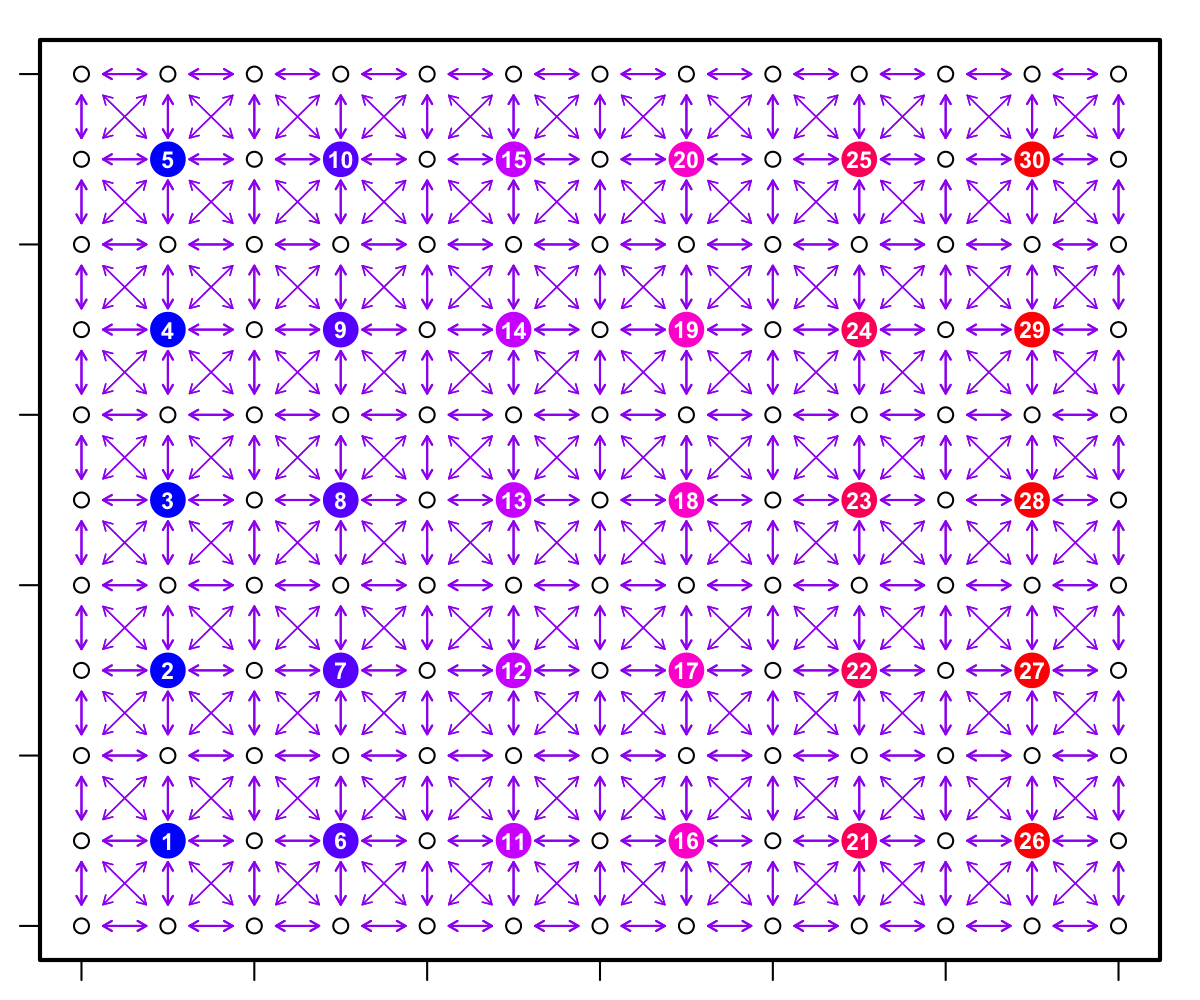
\includegraphics[width=3in,height=2.5in]{figs/sims/basic_lattice.png}}
		\subcaptionbox{Lattice with Barrier \label{barrier_lattice}}
			{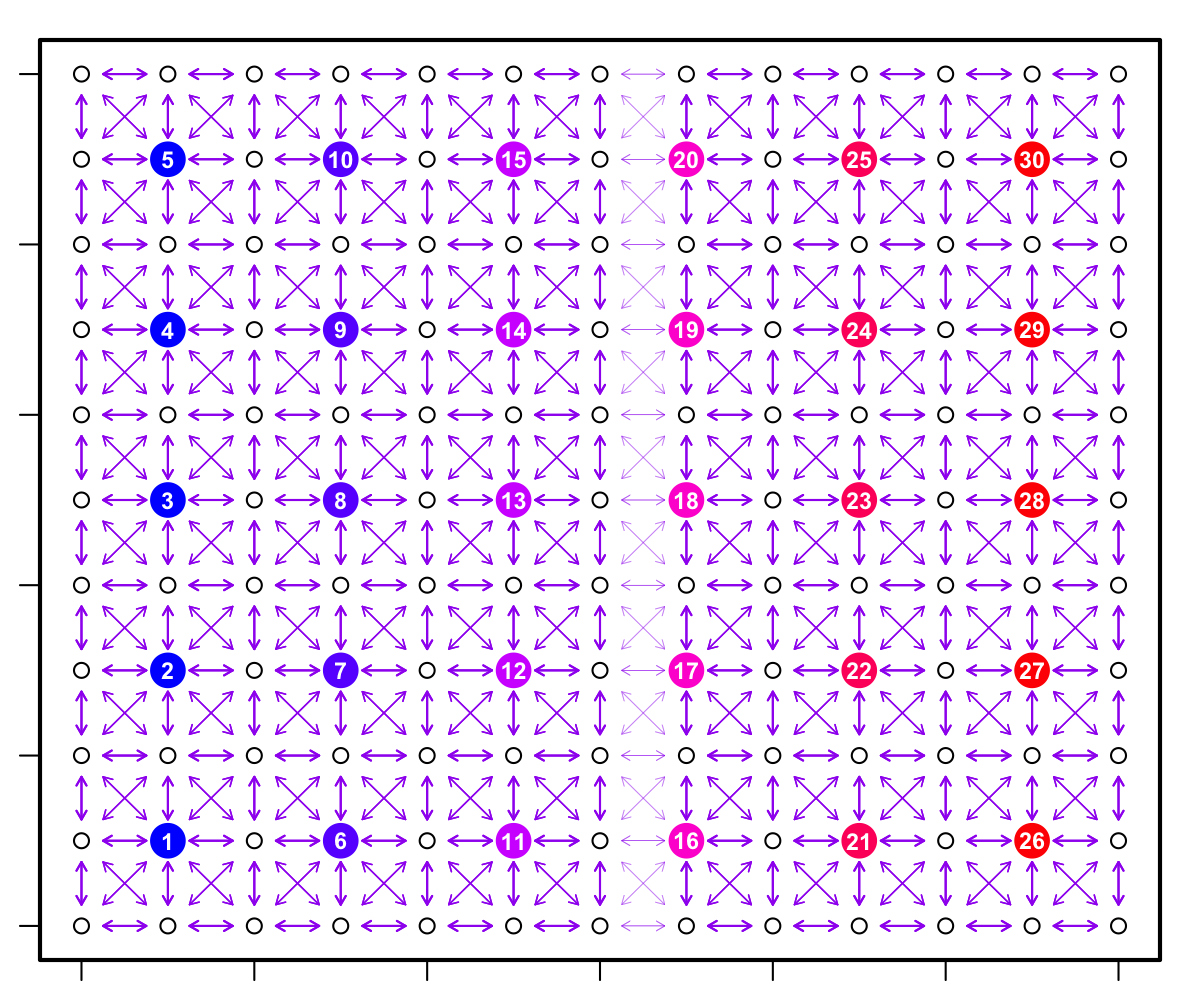
\includegraphics[width=3in,height=2.5in]{figs/sims/barrier_lattice.png}}
		\subcaptionbox{Lattice with Expansion Event \label{barrier_lattice}}
			{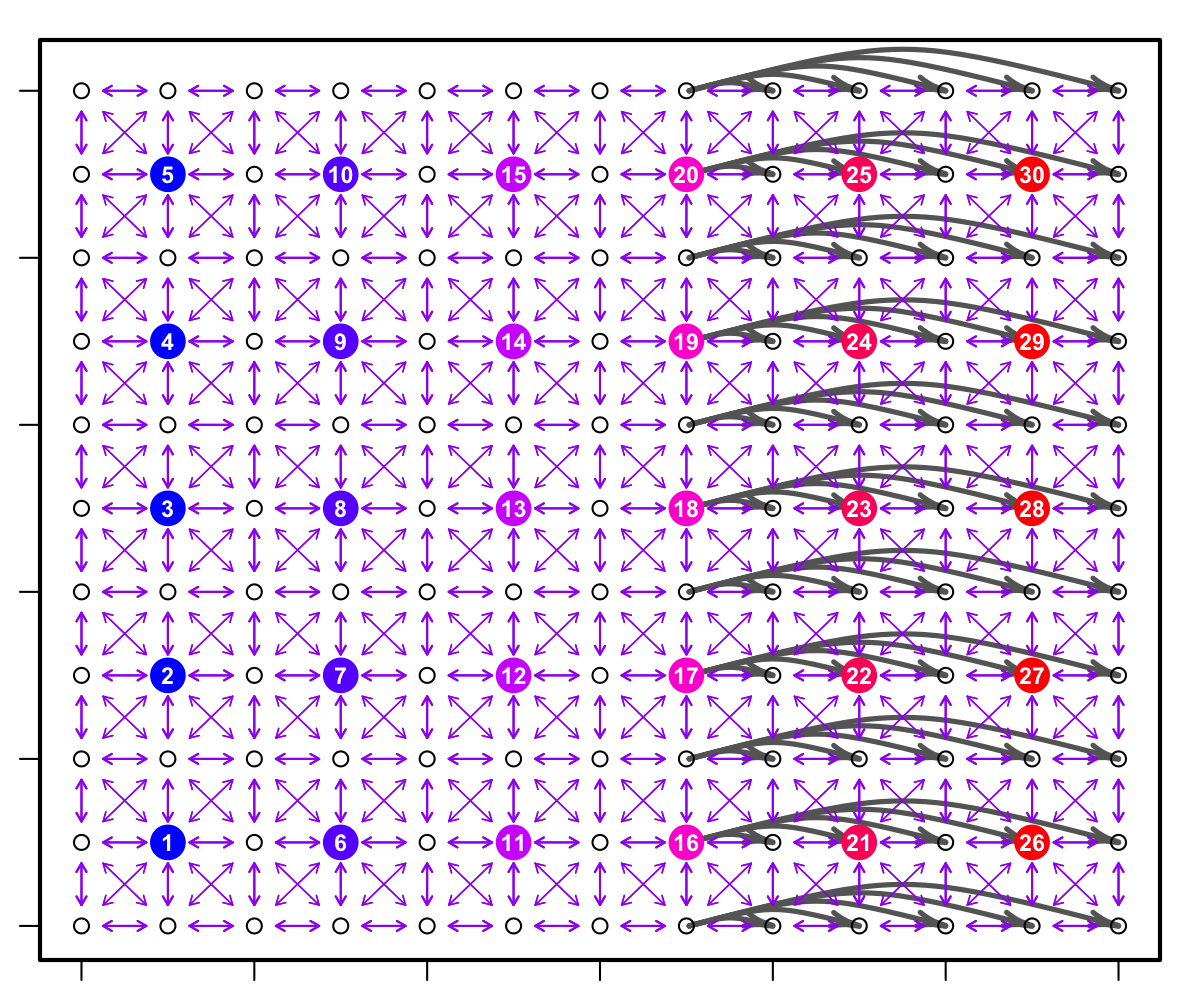
\includegraphics[width=3in,height=2.5in]{figs/sims/expansion_lattice.png}}
	\caption{Different simulation scenarios: (a) basic lattice; (b) lattice with a longitudinal barrier; (c) lattice with expansion event.}\label{sfig:sim_scenarios}
\end{figure}

\begin{figure}[ht!]
	\centering
		{\includegraphics[width=2.4in,height=2in]{figs/sims/GeoGenMap_barr_inland_admixture_2.png}}
	\caption{credible interval of where population 23 draws admixture from.}
\label{sfig:barr_inland_ad_credset}
\end{figure}

\begin{figure}
	\centering
		\subcaptionbox{Lattice \label{lattice_inference}}
			{\includegraphics[width=2.8in,height=2.33in]{figs/sims/GeoGenMap_lattice.pdf}}
		\subcaptionbox{Barrier \label{barrier_inference}}
			{\includegraphics[width=2.8in,height=2.33in]{figs/sims/GeoGenMap_barrier.pdf}}
		\subcaptionbox{Expansion  \label{expansion_inference}}
			{\includegraphics[width=2.8in,height=2.33in]{figs/sims/GeoGenMap_expansion.pdf}}
		\subcaptionbox{Admixture \label{sfig:admixture_inference_CYOL}}
			{\includegraphics[width=2.8in,height=2.33in]{figs/sims/GeoGenMap_corner_admixture_CYOL.pdf}}
	\caption{Population maps inferred using SpaceMix under three different scenarios: a) simple lattice at equilibrium; b) a lattice with a barrier across the center line of longitude; c) a lattice with recent expansion on the eastern margin; d) a lattice with an admixture event between populations 1 and 30.}\label{sfig:lattice_scenarios}
\end{figure}


\begin{figure}
	\centering
		\subcaptionbox{Location Inference \label{sfig:admixture_inference_CYOL}}
			{\includegraphics[width=2.4in,height=2in]{figs/sims/GeoGenMap_corner_admixture_CYOL.pdf}}
		\subcaptionbox{Location and Admixture Inference \label{sfig:admixture_inference_CYOL}}
			{\includegraphics[width=2.4in,height=2in]{figs/sims/GeoGenMap_corner_admixture.png}}
	\caption{Inference of population locations in the scenario depicted in Figure \ref{sfig:admixture_scenario}.  Population 30 has received half of its lineages from population 1, to simulate a long distance admixture event in the very recent past. a) Inference of population locations; b) inference of both population locations and their sources of admixture}\label{sfig:corner_admixture_inference}
\end{figure}

\begin{figure}
	\centering
		\subcaptionbox{Lattice \label{lattice_inference}}
			{\includegraphics[width=2.8in,height=2.33in]{figs/sims/GeoGenMap_lattice.pdf}}
		\subcaptionbox{Barrier \label{barrier_inference}}
			{\includegraphics[width=2.8in,height=2.33in]{figs/sims/GeoGenMap_barrier.pdf}}
		\subcaptionbox{Expansion  \label{expansion_inference}}
			{\includegraphics[width=2.8in,height=2.33in]{figs/sims/GeoGenMap_expansion.pdf}}
		\subcaptionbox{Admixture \label{sfig:admixture_inference_CYOL}}
			{\includegraphics[width=2.8in,height=2.33in]{figs/sims/GeoGenMap_corner_admixture_CYOL.pdf}}
	\caption{Population maps inferred using SpaceMix under three different scenarios: a) simple lattice at equilibrium; b) a lattice with a barrier across the center line of longitude; c) a lattice with recent expansion on the eastern margin; d) a lattice with an admixture event between populations 1 and 30.}\label{sfig:lattice_scenarios}
\end{figure}


\begin{figure}
	\centering
		\subcaptionbox{Location Inference \label{sfig:admixture_inference_CYOL}}
			{\includegraphics[width=2.4in,height=2in]{figs/sims/GeoGenMap_corner_admixture_CYOL.pdf}}
		\subcaptionbox{Location and Admixture Inference \label{sfig:admixture_inference_CYOL}}
			{\includegraphics[width=2.4in,height=2in]{figs/sims/GeoGenMap_corner_admixture.png}}
	\caption{Inference of population locations in the scenario depicted in Figure \ref{sfig:admixture_scenario}.  Population 30 has received half of its lineages from population 1, to simulate a long distance admixture event in the very recent past. a) Inference of population locations; b) inference of both population locations and their sources of admixture}\label{sfig:corner_admixture_inference}
\end{figure}

\begin{figure}[ht!]
	\centering
	\includegraphics[width=2.4in,height=2in]{figs/sims/GeoGenMap_corner_admixture.png}
	\caption{Posterior distribution of inference of the sources and strengths of admixture for the sampled populations.  The admixed population (Population 30) is drawing admixture from the location of its source of admixture that was used to simulate the data (the location of Population 1).}\label{sfigGeoGenMap_corner_admixture}
\end{figure}


\begin{figure}
	\centering
		\subcaptionbox{Simulated Lattice \label{simple_lattice}}
			{\includegraphics[width=2.8in,height=2.33in]{figs/sims/basic_lattice.png}}
		\subcaptionbox{Lattice \label{lattice_inference}}
			{\includegraphics[width=2.8in,height=2.33in]{figs/sims/GeoGenMap_lattice.pdf}}
		\subcaptionbox{Barrier \label{barrier_inference}}
			{\includegraphics[width=2.8in,height=2.33in]{figs/sims/GeoGenMap_barrier.pdf}}
		\subcaptionbox{Expansion  \label{expansion_inference}}
			{\includegraphics[width=2.8in,height=2.33in]{figs/sims/GeoGenMap_expansion.pdf}}
	\caption{Population maps inferred using SpaceMix under three different scenarios: a) configuration of simulated populations; (c) simple lattice at equilibrium; c) a lattice with a barrier across the center line of longitude; d) a lattice with recent expansion on the eastern margin.}\label{sfig:lattice_scenarios}
\end{figure}
%%%Graham's attempts at arrows in equations
%\begin{equation}
%\source{A}~~~~B~~~~ \target{C}~~~~D
%\drawarrows
%\end{equation}
%blah blah

% \begin{equation}
%   A~~~~B\tikzmark{b} ~~~~ C~~~~\tikzmark{a}D
%   \tikz[overlay,remember picture]
%    {\draw[->,square arrow] (a.south) to (b.south);}
% \end{equation}
% blah blah
% \begin{equation}
%   A~~~~B\tikzmark{b} ~~~~ C~~~~\tikzmark{a}D
%   \tikz[overlay,remember picture]
%    {\draw[->,square arrow] (a.south) to (b.south);}
% \end{equation}
 
 
%\newcommand{\tikzmark}[1]{\tikz[overlay,remember picture] \node (#1) {};}
%\tikzset{square arrow/.style={to path={-- ++(0,-.25) -| (\tikztotarget)}}}

%\begin{equation}
 % a\tikzmark{a}x^2 + bx + c = 5\tikzmark{b}x^2 + bx + c.
 % \tikz[overlay,remember picture]
 %  {\draw[->,square arrow] (a.south) to (b.south);}
%\end{equation}


%%Graham's attempts at arrows in equations 
% \newcommand{\tikzmark}[1]{\tikz[overlay,remember picture] \node (#1) {};}
% \tikzset{square arrow/.style={to path={-- ++(0,-.25) -| (\tikztotarget)}}}


% \newcommand\source[1]{%
%     \tikz[remember picture,baseline,inner sep=0pt] {%
%         \node [name=source,anchor=base]{$#1$};
%     }%
%     \setcounter{target}{0}
% }

% \newcounter{target}
% \newcommand\target[1]{%
%     \tikz[remember picture,baseline,inner sep=0pt] {%
%         \node [name=target-\thetarget,anchor=base]{$#1$};
%     }%
%     \stepcounter{target}%
% }

% \newcommand\drawarrows{
%     \tikz[remember picture, overlay, bend left=20, -latex] {
%         \foreach \i [evaluate=\i as \n using int(\i-1)] in {1,...,\thetarget} {
%             \draw (source.north) to (target-\n.north);
%         }
%     }
% }


% \newcommand\newdrawarrows{
%     \tikz[remember picture, overlay, bend left=20, -latex] {
%         \foreach \i [evaluate=\i as \n using int(\i-1)] in {1,...,\thetarget} {
%             \draw (target-\n.north) to (source.north);
%         }
%     }
% }

